\documentclass[11pt,a4paper]{article}
\usepackage[utf8]{inputenc}
\usepackage[german]{babel}
\usepackage{amsmath}
\usepackage{amsfonts}
\usepackage{subcaption}
\usepackage{booktabs}
\usepackage{setspace}
\usepackage{threeparttable}
\usepackage{amssymb}
\usepackage{graphicx}
\usepackage{fancyhdr}
\usepackage[hyphens]{url}
\usepackage{icomma}
\usepackage{float}
\usepackage{pdfpages}
\usepackage{hyperref}
\usepackage{csquotes}
\usepackage[left=2.5cm,right=2.5cm,top=2cm,bottom=3.5cm]{geometry}

\title{\normalsize{Duale Hochschule Baden-Württemberg Karlsruhe}\\
		Fachbereich technische Informatik\\ \vspace{2cm}
		\huge{\textbf{Entwicklung und Erstellung einer }}\\
		\textbf{Dating-App auf Basis von Film- und }\\
		\textbf{Serienpräferenzen für mobile Endgeräte}\\ \vspace{2cm}
		\normalsize{Studienarbeit} von\\
		}
\author{\textbf{Leon Gieringer, Robin Meckler \& Vincent Schreck} \\ \vspace{2cm} \\
		betreut durch \\ \\
		\textbf{Prof. Dr. Kai Becher} \\ \vspace{2cm} \\
		abgegeben am
		}
\date{\today}
\usepackage{wrapfig}
\usepackage{colortbl}
\usepackage{array}



%%%%%%%%%%%% listing & color for Code %%%%%%%%%%%%
\usepackage{color}
\definecolor{lightgray}{rgb}{.9,.9,.9}
\definecolor{darkgray}{rgb}{0.5,0.5,0.5}
\definecolor{ballblue}{rgb}{0.13, 0.67, 0.8}
\definecolor{purple}{rgb}{0.65, 0.12, 0.82}
\definecolor{darkpastelgreen}{rgb}{0.01, 0.75, 0.24}

\usepackage{listings}
\renewcommand*{\lstlistlistingname}{Quellcodeverzeichnis}


\lstdefinelanguage{JavaScript}{
	keywords={typeof, new, true, false, catch, function, return, null, catch, switch, var, if, in, while, do, else, case, break, const, var, from, export, import, defaultValue, class, boolean, throw, implements,this, style},
	keywordstyle=\color{orange}\bfseries,
	ndkeywords={height, borderColor, borderWidth, isHungry, setIsHungry},
	ndkeywordstyle=\color{ballblue}\bfseries,
	identifierstyle=\color{black},
	sensitive=false,
	comment=[l]{//},
	morecomment=[s]{/*}{*/},
	commentstyle=\color{darkgray}\ttfamily,
	stringstyle=\color{darkpastelgreen}\ttfamily,
	morestring=[b]',
	morestring=[b]"
}

\lstset{
	language=JavaScript,
	backgroundcolor=\color{lightgray},
	extendedchars=true,
	basicstyle=\ttfamily,
	showstringspaces=false,
	showspaces=false,
	numbers=left,
	numberstyle=\footnotesize,
	numbersep=9pt,
	tabsize=2,
	breaklines=true,
	showtabs=false,
	captionpos=b
}

%%%%%%%%%%%% titlesec for paragraphs %%%%%%%%%%%%
\usepackage{titlesec}

\setcounter{secnumdepth}{4}
\titleformat{\paragraph}
{\normalfont\normalsize\bfseries}{\theparagraph}{1em}{}
\titlespacing*{\paragraph}{0pt}{3.25ex plus 1ex minus .2ex}{1.5ex plus .2ex}



%%%%%%%%%%%% begin document %%%%%%%%%%%%

\begin{document}
\maketitle
\thispagestyle{empty}
\newpage
\pagenumbering{Roman}
\tableofcontents
\newpage
\listoffigures
\newpage
\listoftables
\newpage
\lstlistoflistings
\newpage
\pagenumbering{arabic}



\pagestyle{fancy}
\fancyhf{}
\setlength{\headheight}{35pt}

\renewcommand\headrulewidth{0.4pt}

\fancyhead[LE,RO]{\rightmark}% <- changed
\fancyhead[LO,RE]{StreamSwipe}
\renewcommand{\sectionmark}[1]{\markright{#1}}
\renewcommand{\subsectionmark}[1]{\markright{#1}}
\renewcommand{\subsubsectionmark}[1]{\markright{#1}}

\cfoot{\thepage}


% Neue Section, neue Seite
\clearpage
\section{Einleitung}
\label{sec:einleitung}

Die Zahl der Scheidungen in Deutschland hat sich während den Einschränkungen durch die COVID-19 Pandemie 2020 verfünffacht \cite{scheidungen}. Neben dem erhöhten Ansturm auf Rechtskanzleien haben sich auch unverheiratete Paare zu Zeiten des Lockdowns getrennt und die Paartherapien sind flächendeckend ausgebucht. Die Menschen suchen sich Partner aus, die sie zwar attraktiv finden, mit denen sie jedoch kaum gemeinsame Interessen und Ansichten teilen. Sind diese Leute gezwungen Zeit miteinander zu verbringen realisieren sie, dass ihre Beziehung nicht passt.\\
Wir wollen diesen gravierenden Fehler in seinem Keim ersticken und revolutionieren das Dating-Game mit einem Verfahren, bei dem persönliche Vorlieben im Vordergrund stehen und das Aussehen zweitrangig ist.



\subsection{Motivation}
Bereits vor tausenden von Jahren haben sich die Menschen Partner gesucht, wobei mit den ersten Fällen der Monogamie auch die erste Beziehung definiert werden kann, in welcher wahrscheinlich auch die ersten Beziehungsprobleme auftraten.\\
Eine der wichtigsten Grundlagen eines harmonischen Zusammenlebens sind gleiche Ansichten, Interessen und Vorlieben. Jedoch ist es nahezu unmöglich einen Partner nach diesen Kriterien  auszusuchen, denn man weiß erst wie gut man zueinander passt, nachdem man sich besser kennengelernt hat. Viele möglicherweise sehr glückliche Beziehungen finden gar nicht statt, da die Person durch ein eigentlich weniger wichtiges Kriterium herausgefiltert wurde. Sucht man die Ursache dieses Problems, ist man schnell bei der Art des Kennenlernens. Der erste Eindruck ist gewöhnlicherweise optischer Natur. Dementsprechend ist Aussehen in der Realität oft der erste Berührungspunk zweier Menschen, was durch StreamSwipe an eine spätere  Position tritt.\\
Wir bieten die Lösung zu einem jahrtausendealten Problem der Menschheit.
%\subsection{Methode}
\subsection{Grundlegende Annahme}
Gerade in den letzten Jahren genießt das Medium Film und Serie einen immer höheren Stellenwert in der Gesellschaft. Durch Video-on-Demand Plattformen wie Netflix, Disney+ und Amazon Prime Video  sind Filme und Serien omnipräsent geworden und das Angebot scheint endlos zu sein. Der Zugriff auf diese Medien wurde dadurch stark vereinfacht und der Nutzer kann einerseits einer Serie oder Filmreihe treu bleiben, da er keine Folge mehr verpassen kann, und andererseits ganze Staffeln an einem einzigen Tag anschauen. So kann dieses Medium bereits bei vielen Menschen eine Charaktereigenschaft werden und Charaktereigenschaften vieler Zuschauer passen sich an Filmcharaktere an.\\
Bereits 2017 haben die 18- bis 39-Jährigen an durchschnittlich 4 Tagen pro Woche eine Serie angeschaut \cite{serienkonsum}. Aus dem Film- und Serienkonsum können somit individualisierte Daten gesammelt und analysiert werden. Bei StreamSwipe wird auf diesem Wege über die Film- und Serienauswahl des Nutzers ein Geschmack berechnet werden, der über einen Algorithmus mit anderen ähnlichen Geschmäcken gematch wird. Sobald ein Match entstanden ist, öffnet sich ein privater Chat und die beiden Personen können sich austauschen und verabreden.

% Neue Section, neue Seite
\clearpage
\section{Theoretische Grundlagen}
\subsection{Netzwerkprotokolle}
\subsubsection{Schichtenmodell}
Eine der gängigsten Arten der Kommunikation findet heutzutage über das Internet statt. 
Dabei handelt es sich um ein weltweit verbundenes Netz von Rechnern. Zur Gewährleistung einer effizienten und geregelten Datenübertragung der heterogenen Computer im Internet wurden Regelwerke, die sogenannten Netzwerkprotokolle, benötigt.
Um das Jahr 1980 wurden daraufhin von verschiedenen Computerherstellern modularisierte Protokolle entwickelt, die fortan als Standard für die digitale Übertragung innerhalb von Rechnernetzen gelten sollen \cite{wikiNetzwerkprotokolle}.
Es musste eine Vielzahl von Aufgaben bewältigt und Anforderung bezüglich Zuverlässigkeit, Sicherheit, Effizienz etc. erfüllt werden. Die Aufgaben reichten dabei von der elektronischen Übertragung der Signale bis zur geregelten Reihenfolge der in der Kommunikation abstrakteren Aufgaben \cite{wikiOsiModell}.
Aus den zu lösenden Problemen und Anforderung kristallisierten sich sieben Schichten bzw. Ebenen heraus. 
Jede einzelne Schicht setzt dabei separat eine Anforderung um und kann dabei durch verschiedene Protokolle realisiert werden. In dem sich etablierten OSI-Schichtenmodell bauen die einzelnen Schichten aufeinander auf, wobei die unterste Schicht das Fundament ist. 
Die Open Systems Interconnection (OSI) wurde von der International Organization for Standardization (ISO), der Internationalen Organisation für Normung, als Grundlage für die Bildung von offenen Kommunikationsstandards entworfen. Das Modell wird in Abbildung \ref{fig:OSISchichten} dargestellt. Die einzelnen Aufgaben werden in der Tabelle \ref{tab:OSISchichtenbeschreibung} beschrieben.\\
\newline
\noindent
Zusätzlich zum OSI-Modell existiert das in den 1960er-Jahren entwickelte TCP/IP-Referenz\-modell. Entwickler dieses Schichtmodells war das Verteidigungsministerium der Vereinigten Staaten, auch bekannt als das Department of Defense (DoD). Dementsprechend trägt das TCP/IP-Referenzmodell auch den Namen DoD-Schichtenmodell \cite{wikiDodModell}.

\begin{figure}[tbt]
\centering
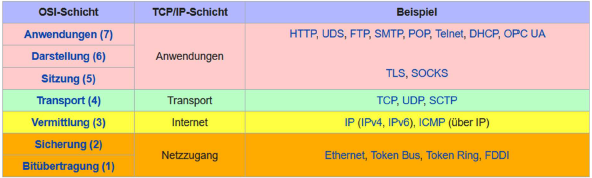
\includegraphics[width=\textwidth]{images/Netzwerkprotokolle_OSI-Schicht.PNG}
\caption[Netzwerkprotokolle: OSI-Schichten]{Netzwerkprotokolle: OSI-Schichten \protect \footnotemark}
\label{fig:OSISchichten}
\end{figure}
\footnotetext{Quelle: \url{https://de.wikipedia.org/wiki/Internetprotokollfamilie}, letzter Zugriff: 06. April 2021}

\newpage

\begin{table}[tbt]
\caption[Kurzbeschreibung der OSI-Schichten]{Kurzbeschreibung der OSI-Schichten \cite{ekOSI}}
\label{tab:OSISchichtenbeschreibung}
\begin{center}
    \begin{tabular}{ l  p{8cm} }
    \toprule
     OSI-Schicht & Aufgabe \\ 
     \midrule
        
    Anwendungen & Funktionen für Anwendungen, sowie die Dateneingabe und -ausgabe \\

    Darstellung & Umwandlung der systemabhängigen Daten in ein unabhängiges Format  \\

    Sitzung & Steuerung der Verbindungen und des Datenaustauschs  \\

    Transport & Zuordnung der Datenpakete zu einer Anwendung \\
    
	Vermittlung & Routing der Datenpakete zum nächsten Knoten \\
	
	Sicherung & Fehlererkennungsmechanismen / Segmentierung der Pakete in Frames und Hinzufügen von Prüfsummen  \\
    
    Bitübertragung & Umwandlung der Bits in ein zum Medium passendes Signal und physikalische Übertragung\\ 
    \bottomrule
    \end{tabular}
\end{center}
\end{table}

\noindent
\hangindent1cm
\textbf{IP:}
In der Vermittlungsschicht des OSI-Schichtenmodells findet, unabhängig des Über\-tra\-gungs\-mediums und der genutzten Topologie, die logische Adressierung der Endgeräte statt. Das geläufigste Protokoll dafür ist das Internet Procotol (IP). Jedem am Netz verbundenen Teilnehmer wird eine IP-Adresse zugewiesen. Die bekannteste Notation ist die 32\,Bit lange IPv4-Adressen und die IPv6-Adressen mit einer Größe von 128\,Bit.\\

\noindent
\hangindent1cm
\textbf{TCP/UDP:}
In der Transportschicht wird eine Ende-zu-Ende-Kommunikation ermöglicht. 
Sie ist das Bindeglied zwischen den anwendungsorientierten und den transportorientierten Schichten. 
Die geläufigsten Protokolle sind das User Datagram Protocol (UDP) und das Transmission Control Protocol (TCP).
UDP ist verbindungslos und daher unzuverlässiger, ist aber durch weniger Overhead belastet.
TCP hingegen ist verbindungsorientiert und dadurch zuverlässiger beim Datentransfer.
Jedes netzwerkfähige Gerät enthält eine Vielzahl von Ports, die primär zur
Unterscheidung zwischen Datenströmen aus Anwendungen bei Netzwerkverbindungen
genutzt werden. Anhand des genutzten Ports bei Netzwerkanfragen
wissen Webserver, welches Protokollverfahren genutzt werden soll.

\noindent
\subsubsection{HTTP}
Das Hypertext Transfer Protocol, kurz HTTP, ist ein zustandloses Protokoll zur Übertragung von Daten auf der Anwendungsschicht. \\

\noindent
\hangindent1cm
\textbf{Kommunikation:}
Unter einer Nachricht versteht man im HTTP Kontext die Kommunikationseinheiten zwischen dem Zentralrechner (Server) und dem, der einen Dienst vom Server abruft (Client). 
Man unterscheidet dabei zwischen der Anfrage (Request) vom Client an den Server und der Antwort (Response) als Reaktion vom Server zum Client. 
\newline
\noindent
Eine Nachricht besteht aus dem Nachrichtenkopf (Message Header, kurz Header) und dem Nachrichtenrumpf (Message Body, kurz Body). 
Der Header enthält generelle Informationen über die Nachricht wie zum Beispiel den Methodentyp, das Datenformat, den genutzten Kompressionsalgorithmus, die Länge der Nachricht oder die verwendete Codierung im Body. 
\newline
\noindent
In Abbildung \ref{fig:HTTPNachricht} ist der Aufbau der HTTP-Nachrichten dargestellt.
Die erste Zeile des Nachrichtenkopfs ist dreiteilig und besteht bei der Anfrage aus dem Namen der Anfragemethode, dem Pfad zur angeforderten Ressource (Uniform Resource Locator, kurz URL) und der verwendet HTTP-Version. Die Anfangszeile einer HTTP-Antwort dagegen besteht zunächst aus der verwendeten HTTP-Version, gefolgt von dem zweiteiligem Status-Code. 
Der Anfangszeile beider Nachrichtentypen folgt eine Reihe von Headerzeilen, wobei jede Zeile aus einem Schlüsselwort/Wert-Paar besteht und die für die Datenübertragung wichtigen Informationen übergibt. 
Der Nachrichtenrumpf, der mit den Nachrichtenkopf über einen Zeilenumbruch syntaktisch voneinander getrennt wird, enthält schließlich die Nutzdaten.
\newline

\begin{figure}[tbt]
\centering
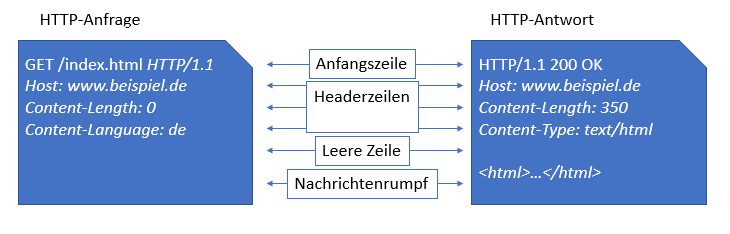
\includegraphics[width=\textwidth]{images/netzwerkprotokolle_http.PNG}
\caption{HTTP-Nachrichtenaufbau}
\label{fig:HTTPNachricht}
\end{figure}

\noindent
\hangindent1cm
\textbf{Methoden:}
HTTP bietet fest definierte Standard-Methoden für Anfragen, die für verschiedene Aufgaben gedacht sind. Im Folgenden werden die wichtigsten Methoden beschrieben:\\

\begin{enumerate}[$\hspace{2cm}\bullet$]
\item \textit{GET} ist die gebräuchlichste Methode. Sie fordert vom Server eine Ressource, die bei Erfolg in der Antwort im Body zurückgegeben wird.
		
\item \textit{POST} ist für die Änderung oder Erzeugung einer Ressource vorgesehen. Dafür werden bei der Anfrage zus"atzlich Daten im Body der Nachricht übertragen.
		
\item \textit{PUT} dient dazu, eine Ressource zu verändern, oder bei Nichtexistenz zu erstellen.
	
\item \textit{PATCH} ändert eine bestehende Ressource ohne diese wie bei PUT vollständig zu ersetzen. 
		
\item \textit{DELETE} löscht die angegebene Ressource auf dem Server.
		
\item \textit{OPTIONS} liefert eine Liste von Methoden und Merkmale, die vom Server unterstützt werden.
\end{enumerate}
\newpage
\noindent
\hangindent1cm
\textbf{Status-Codes:}
HTTP-Antworten senden in der Anfangszeile ihrer Nachricht Status-Codes. Die Angabe ist zweiteilig und besteht aus einer standardisierten Statuskennzahl sowie einer kurzen textuellen Beschreibung, die zusammen Auskunft über den Bearbeitungszustand der zugehörigen Anfrage geben. Tabelle \ref{tab:HTTPStatuscode} stellt die Status-Codes und ihre Beschreibungen anhand von Beispielen dar. \newline

\begin{table}[tbt]
\caption{HTTP Statuscodebeschreibungen}
\label{tab:HTTPStatuscode}
\begin{center}
    \begin{tabular}{ l  l   p{8cm} }
    \toprule
    Typ & Status-Code & Beispiele \\
    \midrule
    
    Informational & 1xx & 100 Continue, 101 Switching\\

    Success & 2xx & 200 OK, 201 Created, 202 Accepted  \\

	Redirection & 3xx & 300 Multiple Choice, 301 Moved Permanently  \\

    Client Error & 4xx & 400 Bad Request, 403 Forbidden\\ 

    Server Error & 5xx & 500 Internal Server Error \\
    \bottomrule
    \end{tabular}
\end{center}
\end{table}

\subsubsection{HTTPS}
Das HTTP-Protokoll hat den großen Nachteil, dass die Nachrichten unverschlüsselt und ungesichert übertragen werden. 
Die Daten können bei der Übertragung von Dritten empfangen, gelesen und verändert werden. Hypertext Transfer Protocol Secure, kurz HTTPS, soll dem entgegenwirken und die Sicherheit bei der Kommunikation gewährleisten. 
Dafür dienen zwei Konzepte:
\newline

\noindent
\noindent
Ersteres ist das Verschlüsseln der Kommunikation von Sender und Empfänger. Die zugrundeliegende Technik nennt sich Transport Layer Security (TLS), ist aber auch als Secure Sockets Layer (SSL) bekannt. Die Idee dahinter ist, dass jeder Teilnehmer der Kommunikation einen öffentlich bekannten Schlüssel (Public Key) und einen geheimen, nicht-öffentlichen Schlüssel (Private Key) besitzt. Über den Public-Key des Empfängers verschlüsselt der Sender seine Nachricht. Diese kann nur über den Private-Key des Empfängers entschlüsselt werden, der vom Empfänger nicht weitergegeben werden sollte.
\newline

\noindent
Das zweite Konzept von HTTPS ist die Webserver-Authentifizierung. Ein Zertifikat, das zu Beginn der Kommunikation an den Webclient gesendet wird, bescheinigt die Vertrauens"-würdig"-keit des Servers. Dafür vertrauen Browser- und Betriebssystemhersteller bestimmten Zertifizierungsstellen, deren Zertifikate sie in ihrem Browser bzw. Betriebssystem hinterlegen. Die Kommunikation zwischen Webserver und Webclient findet folglich erst nach vollständiger Authentifizierung statt.


% Neue Section, neue Seite
\clearpage
\subsection{JavaScript}
In den nächsten Unterkapiteln soll zunächst ein historischer Überblick über die Programmiersprache JavaScript gegeben werden. Im Anschluss wird auf die Bedeutung und Nutzung von JavaScript eingegangen. 
\newline

\subsubsection{Historie}
Ihren Ursprung findet die Programmiersprache JavaScript im Jahr 1995, als Brendan Eich, ein damaliger Ingenieur des US-amerikanischen Software-Unternehmens „Netscape Communications Corporation“, innerhalb von zehn Tagen diese Sprache für den Browser „Netscape Navigator“ entwickelt hat \cite{JS1}. Das Ziel dabei war es, eine Skriptsprache zu entwickeln, die es Entwicklern möglich machen sollte, auf ihren Webseiten Skripte umzusetzen. Zunächst noch unter dem Namen Mocha und LiveScript änderte sich der Name zu JavaScript aufgrund der Kooperation von Netscape und Sun, der Firma hinter der Programmiersprache Java, und Marketinggründen. Netscape wollte von der damaligen Popularität von Java profitieren \cite{JS1.05}. 
\newline
\noindent
Netscape’s Veröffentlichung des Netscape Navigator 2.0, der erste Browser der JavaScript unterstützte, brachte Microsoft dazu, Netscape als ernstzunehmenden Konkurrenten zu sehen. 
Microsoft antwortete im August 1995 mit der Veröffentlichung des ersten Internet Explorer zusammen mit der Skriptsprache JScript, die einen Dialekt der Sprache JavaScript darstellt. Dies ist ferner als der Beginn der „Browserkriege“ bekannt\cite{JS1.06}.
\newline
\noindent
Im Jahre 1997 reichte Netscape JavaScript an die European Computer Manufacturers Association (kurz ECMA), einer privaten, internationalen Normungsorganisation zur Normung von Informations- und Kommunikationssystemen und Unterhaltungselektronik, ein. Das Ziel war es, von der ECMA einen einheitlichen Standard für die Sprache schaffen zu lassen, die fortan weiterentwickelt werden und von weiteren Browserherstellern genutzt werden soll. Das resultierende Standard nennt sich ECMAScript, wobei JavaScript die bisher bekannteste Implementierung dieses Standards ist\cite{JS1.07}. 
Andere Implementierungen sind zum Beispiel ActionScript von Macro\-Media, JScript von Microsoft und ExtendScript von Adobe.
\newline
\noindent
Jährlich wird dieser Standard seit Juni 2015 erweitert. ECMAScript Version 11 beziehungs\-weise ECMAScript 2020 bildet zum Zeitraum dieser Dokumentation den aktuellen Standard \cite{JS1.08}. 
Im Juni 2021 soll die neueste Version ECMAScript 2021 veröffentlicht werden \cite{JS1.09}. 
\newline

\subsubsection{Wesentliche Programmiereigenschaften}
„JavaScript is Not Java“  \cite{JS1.091}. Die Programmiersprache JavaScript wird aufgrund ihrer Namensgebung oft in falsche Zusammenhänge zu Java gebracht. Das häufigste Missverständnis sei, JavaScript wäre eine vereinfachte Version von Java \cite{JS1.091}.
\newline
\noindent
JavaScript ist eine interpretierte Programmiersprache mit objektorientierten Umsetzungs\-möglichkeiten. Interpretation ist in diesem Zusammenhang so zu verstehen, dass der Quellcode zur Laufzeit eines Programms gelesen, übersetzt und ausgeführt wird.
Syntaktisch ähnelt JavaScript kompilierten Programmiersprachen wie C, C++ und Java durch gleiche Umsetzung der Kontrollstrukture wie den Bedingungen, Schleifen oder den booleschen Operatoren \cite{JS1.1}. Wesentliche Unterschiede sind dagegen, dass JavaScript zum einen eine schwach-typisierte Sprache ist. Durch die schwache Typisierung haben Variablen keinen festen Dateityp und können diesen dynamisch zur Laufzeit ändern. Des Weiteren findet bei JavaScript die Objektorientierung prototypenbasiert statt. Diese Form der Programmierung wird auch klassenlose Objektorientierung bezeichnet. Anders als bei der klassenbasierten Programmierung, bei der Objekte aus vor\-de\-fi\-niert\-en Klassen instanziiert werden, werden hier Objekte durch Klonen bereits existierender Objekte erzeugt. Die Objekte, die geklont werden, sind dabei als Prototyp-Objekte zu ver\-steh\-en. Beim Klonen werden alle Attribute und Methoden des Prototyp-Objekts in das neue Objekt übernommen und können dort überschrieben sowie erweitert werden. Objekte in JavaScript sind eher als Zuordnungslisten, ähnlich wie assoziative Arrays oder Hash-Tabellen, anzusehen, da bei der Eigenschaftszuweisung lediglich ein Mapping eines Schlüsselworts (Key) zu seiner zugehörigen Eigenschaft ( Value) stattfindet, wie es in Abbildung \ref{fig:JavascriptObjekt} zu sehen ist.
\newline

\begin{figure}[tbt]
\centering
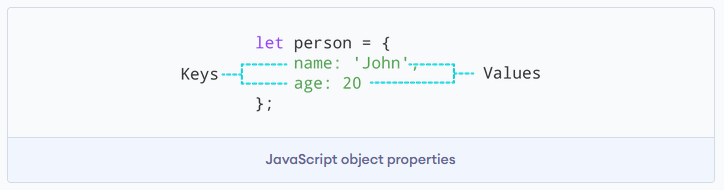
\includegraphics[width=\textwidth]{images/JavaScript_Object.PNG}
\caption[JavaScript Objekt]{JavaScript Objekt \cite{JS1.29}}
\label{fig:JavascriptObjekt}
\end{figure}



Ein weiterer Unterschied zu den anderen Programmiersprachen ist, dass alle Funktionen und Variablen außer der primären Datentypen Boolean, Zahl und Zeichenfolge, als Objekte verstanden werden können.

\subsubsection{Anwendungsgebiete}
Ursprünglich fand JavaScript seinen Einsatz hauptsächlich darin, dynamische Webseiten im Web\-browser anzuzeigen. Die Verarbeitung erfolgte dabei meist clientseitig durch den Webbrowser (dem sogenannten Frontend) \cite{JS1.3}.
\newline
\noindent
Heutzutage findet sich die Sprache dagegen in wesentlich größeren Einsatzgebieten wieder. 
Bis vor einigen Jahren war die Serverseite anderen Programmiersprachen wie Java oder PHP vorbehalten. Die Veröffentlichung von Node.js, einer plattformübergreifenden Laufzeitumgebung, die JavaScript außerhalb eines Webbrowsers ausführen kann, führte zu einer immer größeren Verbreitung von serverseitigen Anwendungen (dem Backend), die auf JavaScript basieren. Auf Node.js wird ausführlicher im nächsten Kapitel eingegangen. 
Ferner findet JavaScript heutzutage aber auch seinen Einsatz in mobilen Anwendungen, Desktopanwendungen, Spielen oder 3D-Anwendungen \cite{JS1.4}.



% Neue Section, neue Seite
\clearpage
\subsection{Node.JS}
Im Jahr 2009 veröffentlichte Ryan Dahl das Framework Node.js, das auf Googles V8-Engine, welche auch als JavaScript-Engine in Googles Browser Chrome zum Einsatz kommt, basiert und sich hervorragend für hochperformante, skalierbare und schnelle Webanwendungen eignet. Zudem ermöglicht es Webentwicklern die Entwicklung von serverseitigem JavaScript-Code\footnote{\url{https://v8.dev/}, letzter Zugriff: 03. April 2021}.


\subsubsection{Architektur}
Eine wesentliche Eigenschaft von Node.js ist die hohe Performance. Im Folgenden soll der Unterschied der Node.js-Architektur zu traditionellen Webservern und der damit verbundenen höheren Performance dargestellt werden.
\newline

\noindent
Herkömmliche Webserver erstellten zunächst für jede ankommende Anfrage einen neuen Thread. Dieses Vorgehen ist eng mit steigendem Speicher- und Rechenaufwand verbunden. Um sich Rechenzeit, die durch die Erstellung und Zerstörung von Threads entstanden, zu sparen, wurden Threadpools eingerichtet. Dieser Threadpool enthält mehrere Threads, denen Aufgaben zugewiesen werden können. Nach erfolgreicher Abarbeitung einer Operation kann einem Thread eine weitere Aufgabe zugeordnet werden.
\newline

\noindent
Es bleibt aber ein weiteres Problem: Bei der Anfragenabarbeitung kann es zu einer Form von blockierender Ein- und Ausgabe (Blocking Input/Output kurz Blocking I/O) kommen: zum Beispiel beim Suchen in einer Datenbank oder dem Laden einer Datei im Dateisystem.
 Während der Abarbeitung wartet der Thread solange, bis die Operation ein Ergebnis zurückwirft und belegt dabei weiterhin Speicherplatz. 
 Bei hohem Aufkommen von Anfragen kommt es dadurch zu einer hohen Speicherauslastung des Servers. Zudem kosten die Kontextwechsel zwischen den Threads im Betriebssystem weitere Rechenzeit \cite{Node1.05}. Man spricht bei diesem Architekturkonzept auch vom Multi-Threaded Server. Graphisch dargestellt ist das Konzept in Abbildung \ref{fig:Multithreaded}.
\newline

\begin{figure}[tbt]
\centering
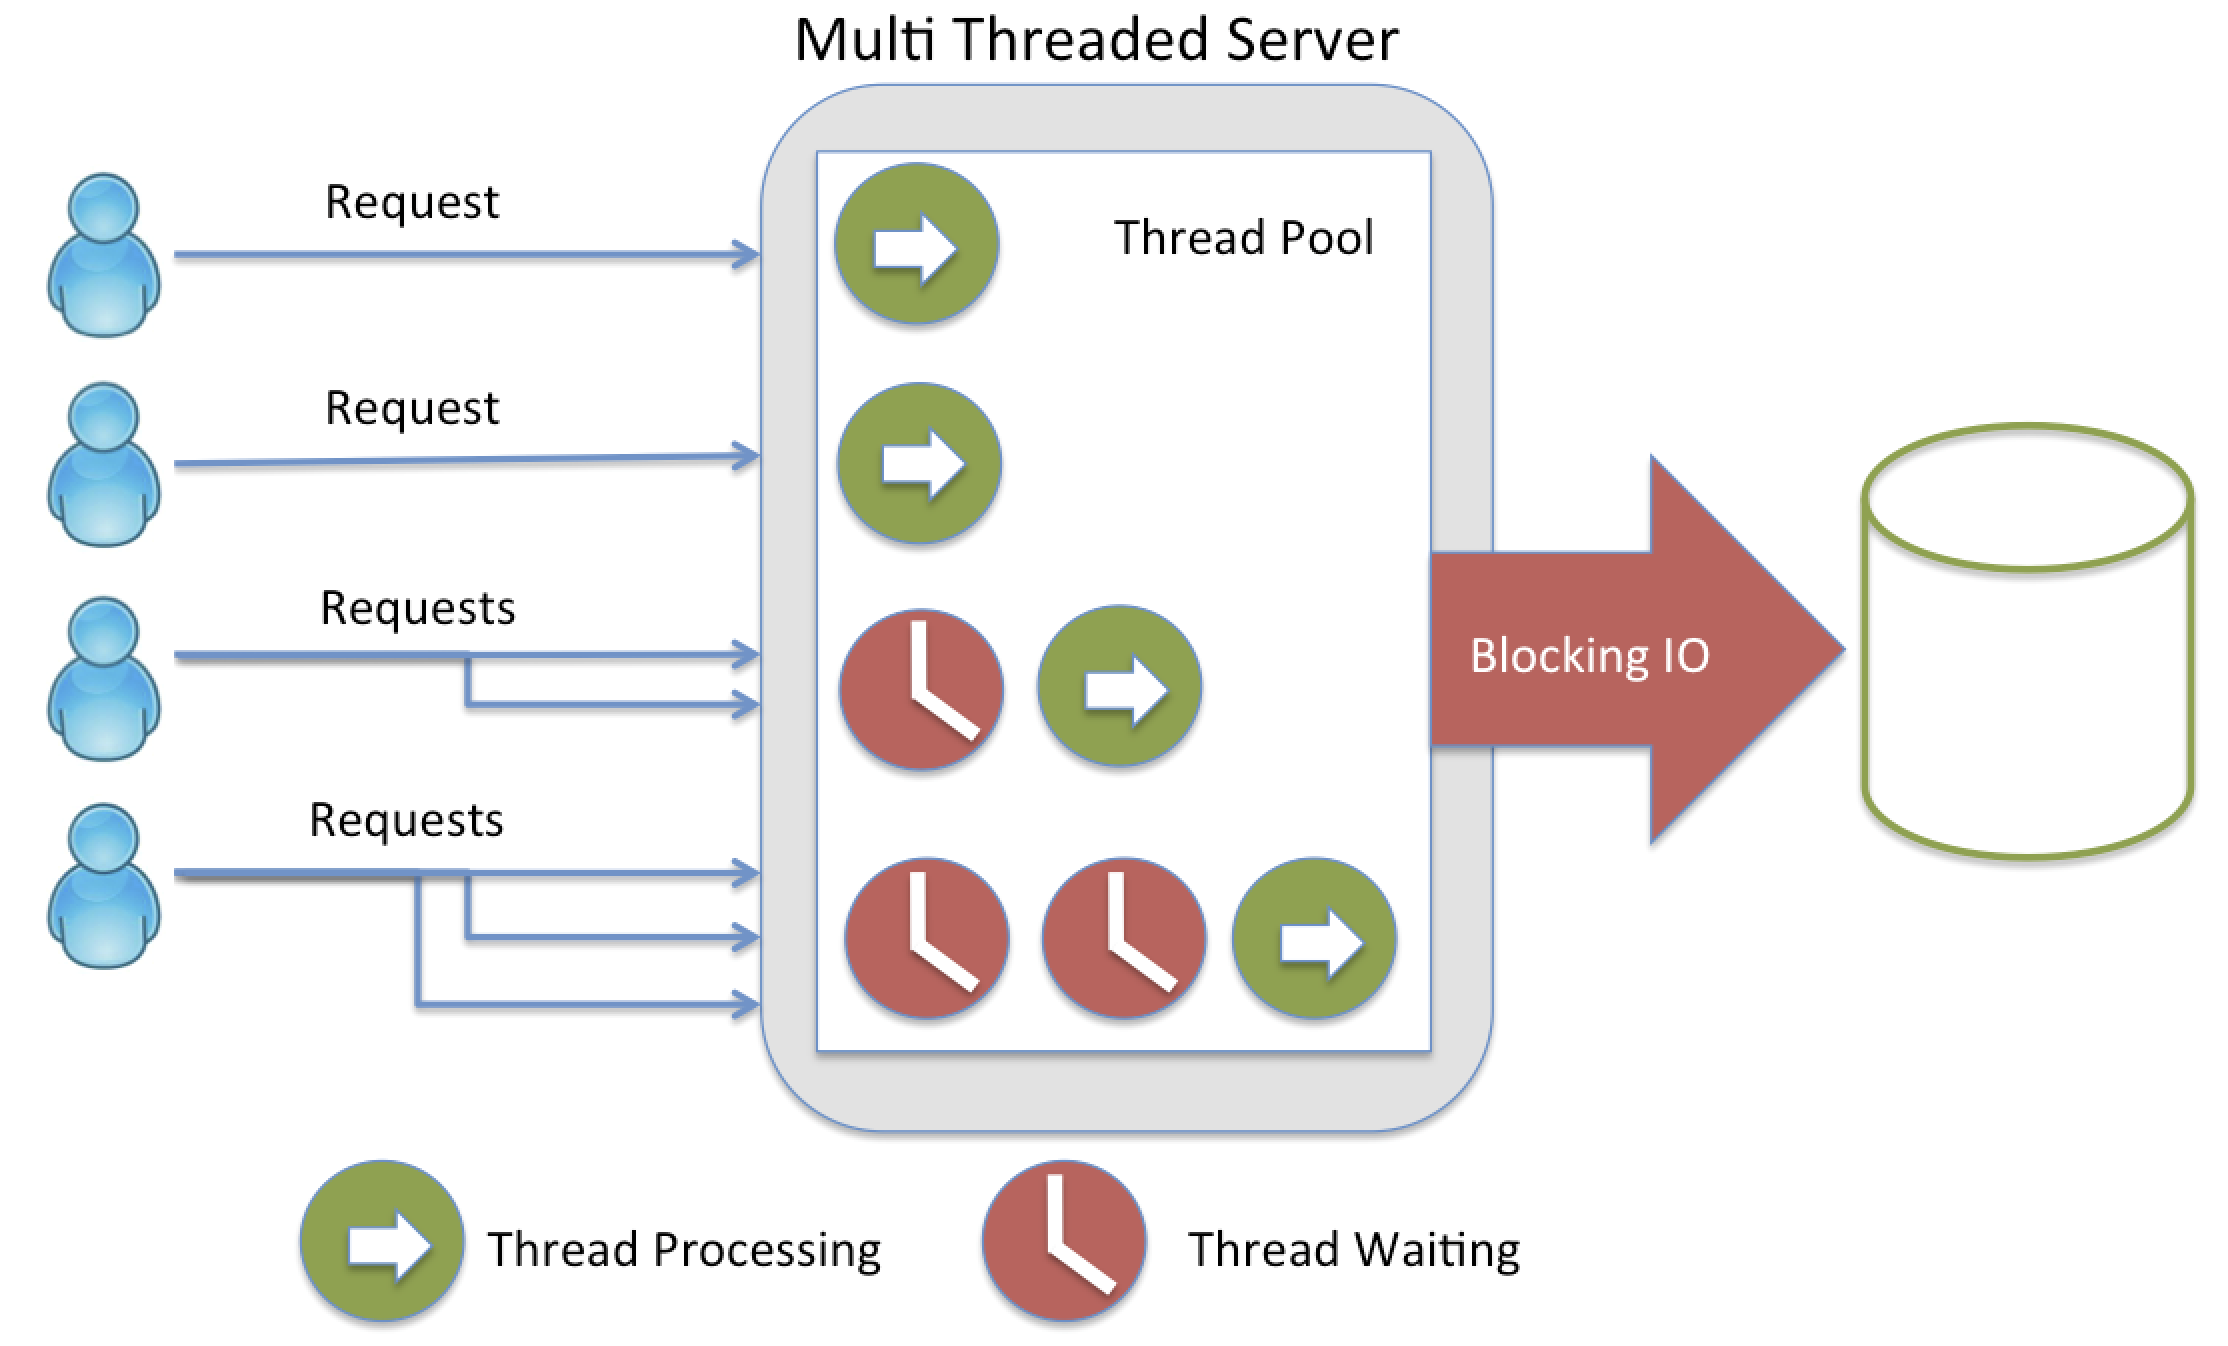
\includegraphics[width=10cm, height = 5.5cm]{images/nodejs_otherthreading.png}
\caption[Multithreaded / Blocking I/O]{Multithreaded / Blocking I/O \cite{Node1.1}}
\label{fig:Multithreaded}
\end{figure}
 
\newpage

\noindent
Node.js verfolgt einen anderen Ansatz: Wie in Abbildung \ref{SingleThreaded} dargestellt, werden Anfragen nur in einem einzigen Thread, dem Hauptthread, abgearbeitet und in einer Warteschlange verwaltet. Dadurch bleiben Kontextwechsel zwischen Threads erspart. Hierbei handelt es sich also um einen Single-Threaded Server. Der Hauptthread verwaltet eine Schleife, die sogenannte Event Loop, die permanent Anfragen aus der Event-Warteschlange überprüft und Ereignisse, die von Ein- und Ausgangsoperationen ausgerufen werden, verarbeitet.
\newline

\noindent
Bei Ankommen einer Nutzeranfrage an einen Node.js Server wird zunächst in der Event Loop geprüft, ob diese Anfrage Blocking I/O benötigt. Falls nicht, kann die Anfrage direkt bearbeitet werden und die Antwort an den Nutzer zurückgesendet werden. 
\newline

\noindent
Im anderen Fall wird einer von Node.js interner Workern, welche prinzipiell auch Threads sind, aufgerufen, um die jeweilige Operation auszuführen. Dabei wird eine Callback-Funktion mitgegeben, die vom Worker aufgerufen wird, sobald die Operation ausgeführt wurde. Diese Callback-Funktion kann anschließend als Ereignis von der Event Loop registriert werden. Man spricht hierbei auch von ereignisgesteuerter Architektur. [1.4]
\newline
 
\begin{figure}[tbt]
\centering
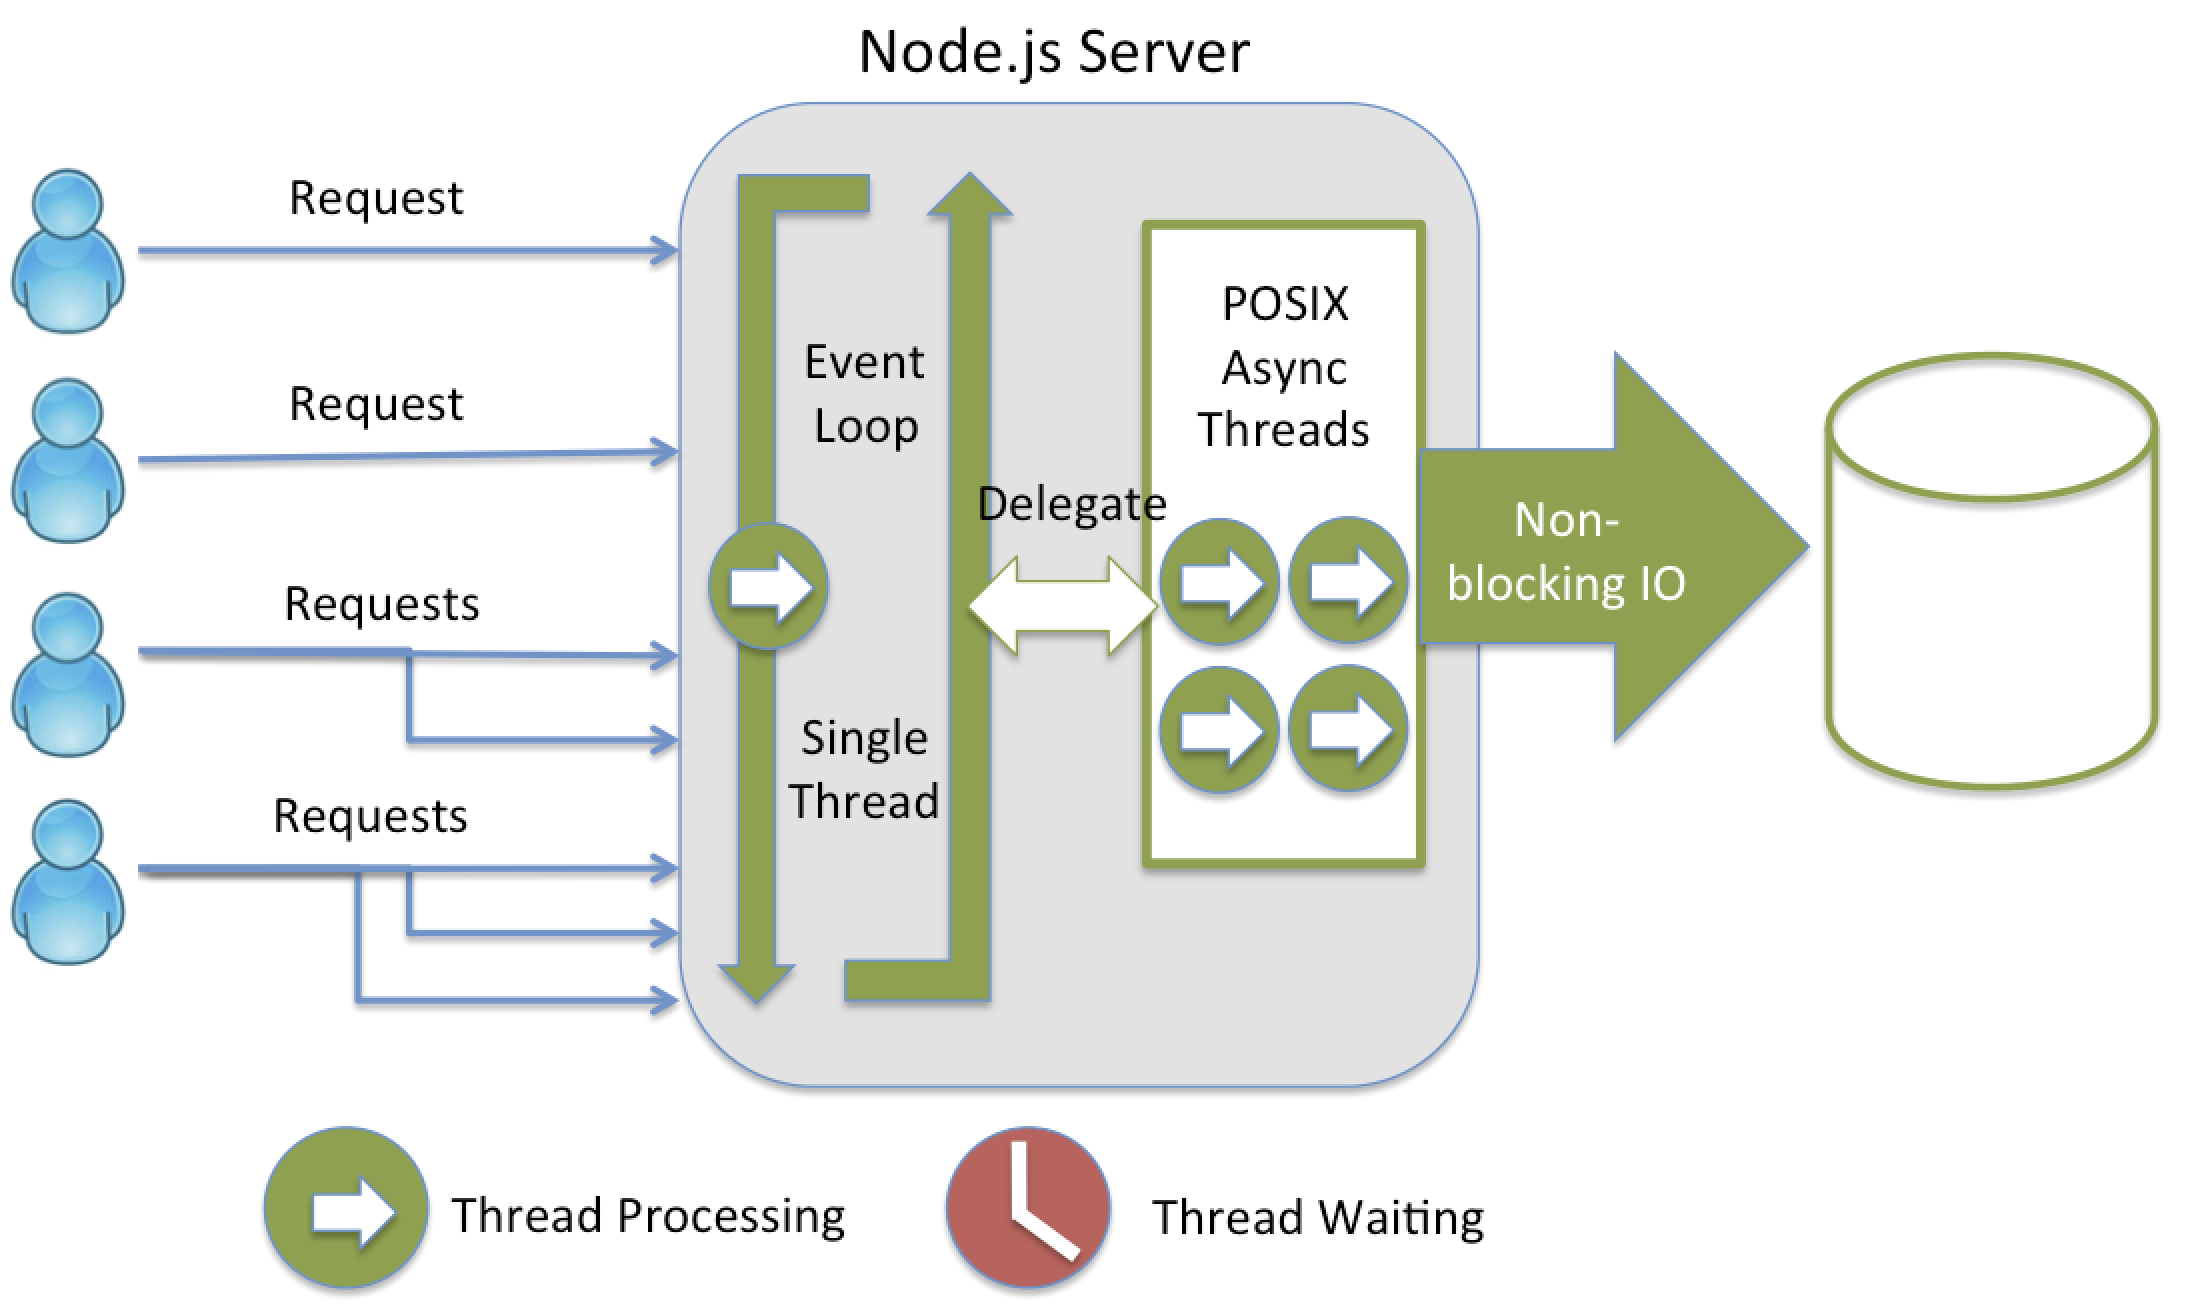
\includegraphics[width=10cm, height = 5.5cm]{images/nodejs_nodethreading.png}
\caption[Single Threaded / Non Blocking I/0]{Single Threaded / Non Blocking I/0 \cite{Node1.1}}
\label{SingleThreaded}
\end{figure}
 

\noindent
Der große Vorteil hierbei ist, dass der Hauptthread trotz der blockierenden Ein- und Aus\-gabeoperationen nicht anhält, und weitere Anfragen bearbeiten kann. (Non Blocking I/O - Prinzip) 
\newline

\newpage
\subsubsection{Module}

\noindent
Module stellen in Node.js Software-Komponenten dar, die Objekte und Funktionen nach außen hin bereitstellen sollen.
Sie können aus einer Skriptdatei oder einem Verzeichnis von Dateien bestehen. Module können als einzelne Default-Komponenten, die den Hauptteil des Moduls repräsentiert, exportiert werden. 
Bei der anderen Möglichkeit, des sogenannten ‚benannten Exports‘ werden die zu exportierenden Komponenten dagegen explizit angegeben. Letzteres ist in nachfolgender Abbildung dargestellt. 
\newline
  
    
\begin{lstlisting}[caption=Benannter Export von Modulen,label=lst:ModuleExport]
function foo(){}
function bar(){}

//Obige Funktionen exportieren:
module.exports.foo = foo;
module.exports.bar = bar;
\end{lstlisting}


\noindent
Für den Import stehen verschiedene Möglichkeiten zur Verfügung.
Im folgender Abbildung ist ein Import über die require()-Funktion dargestellt. 
Mit mitgeliefertem Modul-Pfad als Parameter gibt diese Funktion ein Objekt des Moduls wieder, das die exportierten Objekte (und Funktionen) enthält.
\newline
  
\begin{lstlisting}[caption=Import von Modulen,label=lst:ModuleImport]
//Importieren der Funktion einer anderen Datei:
const foo = require('./module/path');
const bar = require('./module/path');
\end{lstlisting}

\noindent
Eine wichtige Besonderheit ist, dass importierte Module  beim ersten Aufruf gecached werden. 
Das bedeutet, dass jeder require()-Aufruf auf ein Modul dasselbe Objekt zurückliefert \cite{Node1.21}.


\paragraph{npm}
Ehemals als Node Package Manager bekannt, ist npm ein Paketmanager für Node.js, entwickelt 2010 von Isaac Z. Schlueter \cite{Node1.3}. Es verwaltet ein öffentliches Repository (ein digitales Software-Verzeichnis im Internet) unter dem Name npm Registry. In dem Verzeichnis werden weit über 1 Millionen Pakete (Module) angeboten \cite{Node1.4}. Der Großteil kann unter freier Lizenz verwendet werden. Mit npm können Module installiert, aktualisiert, entfernt und gesucht werden. Node.js liefert seit seiner Version 0.6.3 npm standardmäßig bei der Installation mit \cite{Node1.5}.

\paragraph{Express}
„Express ist ein einfaches und flexibles Node.js-Framework von Webanwendungen, das zahlreiche leistungsfähige Features und Funktionen für Webanwendungen und mobile Anwendungen bereitstellt“ \cite{Node1.6}.  Es wurde im November 2010 von Douglas Christopher Wilson und weiteren Entwicklern veröffentlicht und erweitert Node.js um das Abarbeiten verschiedener HTTP-Methoden, das separate Abarbeiten von Anfragen mit verschiedenen URL-Pfaden sowie weiterer nützlicher Möglichkeiten. Im Grunde handelt es sich bei Express um ein Modul, dass durch den npm Package Manager heruntergeladen werden kann. Die aktuelle Version zum Zeitpunkt der Dokumentation ist 4.17.1 \footnote{\url{https://www.npmjs.com/package/express}, letzter Zugriff: 04. April 2021}
\newline
\newline
\textbf{Beispiel}
\newline

\noindent
Das Erstellen einer einfachen Express-Applikation wird im folgenden Beispiel dargestellt:\newline

\begin{lstlisting}[caption=Einfacher Webserver [nodejs 1.8],label=lst:Middleware]
const express = require('express');
const app = express();
const port = 3000;

app.get('/', (req,res)=> {
	res.send('Hello World')
});

app.listen(port, () => {
	console.log("Example app listening on port ${port}!")
});
\end{lstlisting}

\noindent
Die require()-Funktion importiert das Express-Modul und gibt ein Express-Objekt zurück. 
Dieses Objekt als Funktion aufgerufen gibt wiederum ein Objekt der Express-Applikation zurück, welche traditionell „app“ genannt wird, das Kernstück des Express-Frameworks ist und sämtliche Methoden wie das Weiterleiten von HTTP Anfragen, das Konfigurieren von Middleware oder das Modifizieren des Webserver-Verhaltens beinhaltet \cite{Node1.8}.
\newline
\noindent
Im mittleren Block befindet sich eine Routendefinition. Die app.get() Funktion spezifiziert eine Callback-Funktion, die ein „request“- und „response“-Objekt als Parameter erhält und aufgerufen wird, sobald eine HTTP Anfrage der Methode GET mit dem Pfad ‚/‘ empfangen wird. Das Request-Objekt enthält sämtliche Informationen über die HTTP-Anfrage. Das Response-Objekt kann dagegen in der Callback-Funktion mit Informationen gefüllt werden und über die send()-Funktion als HTTP-Antwort an den Sender zurückgesendet werden.
\newline
\noindent
Der unterste Block startet den Webserver auf dem mitgegebenen Port über die Funktion app.listen(). Ihr kann auch eine Callback-Funktion mitgegeben werden, die aufgerufen wird, sobald der Server erfolgreich gestartet ist.
\newpage

\noindent
\textbf{Middleware:}
Express arbeitet nach dem Middleware-Konzept. Darunter versteht man Funktionen, die für die Verarbeitung von Anfragen hintereinandergeschaltet werden können. Jede Middleware hat Zugriff auf das Anfrageobjekt, das Antwortobjekt und die jeweils nächste Middleware-Funktion \cite{Node1.9}.
Dabei kann die HTTP-Request direkt terminiert oder an die nächste Middleware gesendet werden. Die Verkettung der Middleware-Funktionen wird in Abbildung \ref{fig:middleware} illustriert.
\newline

\begin{figure}[tbt]
\centering
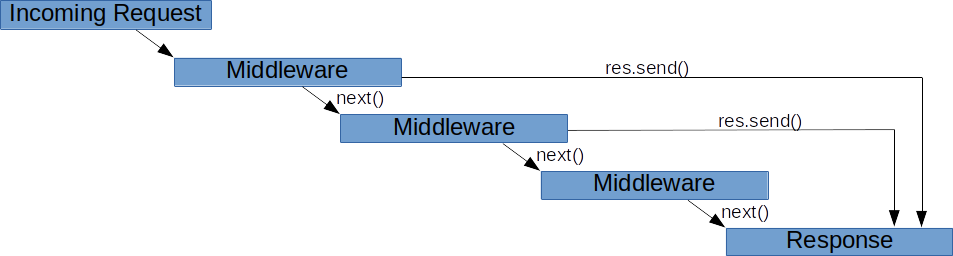
\includegraphics[width=12cm]{images/nodejs_middleware.png}
\caption[Middleware]{Middleware \cite{Node1.2}}
\label{fig:middleware}
\end{figure}

%
%       Middleware
%			express.json
%

\noindent
\textbf{express.json:}
Hierbei handelt es sich um eine in express eingebaute Middleware, die die in JSON formatierten Daten im Nachrichtenrumpf aus einer eingehenden HTTP-Anfrage grammatisch analysiert.  Dabei ist zu beachten, dass der Nachrichtenrumpf nur dann analysiert wird, wenn bei der Anfrage eine Header-Informationen namens „Content-Type“ mit dem entsprechenden JSON-Typ als Wert übergeben wird. Nach erfolgreicher Analyse erstellt die Middleware aus den JSON-Informationen eine neues body-Objekt innerhalb des übergebenen request-Objekts \cite{Node2.1}.
\newline

\begin{lstlisting}[caption=Express.json Middleware benutzen,label=lst:ExpressNutzen]
const express = require('express');
const app = express();
app.use(express.json());
\end{lstlisting}

%
%       Middleware
%			Router
%

\noindent
\textbf{Router:}
Unter dem Begriff Routing (Weiterleitung) versteht man im Kontext von Express „[...] die Definition von Anwendungsendpunkten (URIs) und deren Antworten auf Clientanforderungen.“ [nodejs 2.15]
\newline

\noindent
Die in express eingebaute Middleware express.Router ermöglicht es, modular einbindbare Routenhandler (Weiterleitungsroutinen) zu erstellen. Eine Router-Instanz ist als vollständiges Middleware- und Routingsystem zu sehen und wird deshalb auch als „Mini-App“ angesehen. Der sich durch die Modularität herausziehende Vorteil ist, dass folglich unterschiedliche Anwendungsendpunkte auf entsprechende Dateien ausgelagert werden können.
\newline

\begin{lstlisting}[caption=Routinghandler erstellen \protect \footnotemark,label=lst:RoutingHandlerCreate]
var express = require('express');
var router = express.router();

// Middleware explizit fuer diesen Router
router.use(function timeLog(req,res,next) {
	console.log('Time: ', Date.now());
	next();
});

// Homepage Route - Abhandlung
router.get('/', function(req,req){
	res.send('Birds home page');
});

// About Route - Abhandlung
router.get('/about', function(req,req){
	res.send('About birds');
});
module.exports = router;
\end{lstlisting}
\footnotetext{Express, API-Dokumentation Router. \url{https://expressjs.com/en/api.html\#router}, letzter Zugriff: 05. April 2021}

\noindent
In oberem Beispiel wird ein Routerhandler für das Verzeichnis ‚/birds‘ mit eigen implementierter Middleware und zwei Anwendungsendpunkte ‚/‘ (bezieht sich auf das Stammverzeichnis) und ‚/about‘ erstellt. Der Code wird unter der Datei birds.js abgespeichert. 
Abschließend kann das Routermodul in die Anwendung geladen werden: 
\newline

\begin{lstlisting}[caption=Routinghandler benutzen,label=lst:RoutingHandlerUsage]
var birds = require('./birds');
..
app.use('birds', birds);
\end{lstlisting}

%
%       Mongoose
%
%

\newpage
\paragraph{Mongoose}
Mongoose ist ein öffentliches Modul, das zum Zeitpunkt der Dokumentation im npm Package Manager in der Version 5.12.3 zur Verfügung steht \footnote{npm mongoose. \url{https://www.npmjs.com/package/mongoose}, letzter Zugriff: 05. April 2021}. Bei diesem Modul handelt es sich um ein Object-Document Mapper (ODM), der es ermöglicht, asynchron mit einer NoSql-Datenbank zu kommunizieren. Mongoose ist der populärste und am weitest von MongoDB unterstützte ODM \cite{Node2.55}. Es unterstützt neben transparenter Persistenz auch die Datenvalidierung, das Erstellen von Abfragen (Queries), das Schreiben von logischem Business Code und die Übertragung zwischen Objektem im Code und der Repräsentierung dieser Objekte in der Datenbank.
\newline

%
%       ODM
%
%

\noindent
\textbf{Object Document Mapping (ODM):}
Object-Relational Mappers (ORM) finden haupt\-sächlich Einsatz in objektorientieren Anwendungen, dessen Daten in relationalen Datenbanken sind. Dabei werden die Tabellen in persistente Objekte gemappt.
Das Mappen ist aber auch für NoSQL-Datenbanken nützlich \cite{Node2.56}. Die meistverbreiteten NoSQL-Datenbanken basieren auf Dokument-Systemen. Dementsprechend werden für diese Datenbanken Object-Document Mapper für das Mappen zwischen Dokumenten und Objekten genutzt. Einige ODM’s sind Mongoose\footnote{Mongoose Webpage, \url{http://mongoosejs.com}, letzter Zugriff: 04. April 2021}, Morphia\footnote{Morphia Webpage, \url{https://github.com/mongodb/morphia}, letzter Zugriff: 04. April 2021}, Doctrine \footnote{Doctrine Project Webpage, \url{http://www.doctrine-project.org/}, letzter Zugriff 04.04.2021} und Mandango\footnote{Mandango Webpage, \url{https://mandango.readthedocs.io/en/latest/}, letzter Zugriff: 04. April 2021.}
NoSQL Mapper nutzen vom Entwickler definierte Datenschemata, die das Objekt beschreiben. Ein daraus abgeleitetes Model-Objekt ermöglicht dann die Kommunikation zwischen dem im Schema beschriebenen Objekt und der entsprechenden Datenbank-Collection.
\newline

%
%       Schema
%
%

\noindent
\textbf{Schema:}
Mongoose-Schemata definieren die Struktur der gespeicherten Daten einer Mongo"-DB-"-Collection in der Anwendungsschicht und werden in der JSON-Notation beschrieben. Dokumentenbasierte Datenbanken wie MongoDB enthalten für jede Wurzelentität eine Collection. Mongoose Schemata werden für jede Collection definiert. Innerhalb der JSON-notierten Schemabeschreibung können den einzelnen Eigenschaften bestimmtes Verhalten zugeordnet werden. Zum Beispiel lässt sich explizit der Datentyp angeben (type), eine Eigenschaft verpflichtend (required) oder in Kleinbuchstaben einstellen (lowercase).
\newline


\begin{lstlisting}[caption=Mongoose Schema - Beispiel,label=lst:MongooseSchema]
const schema = new Schema({
 attributeX: {
 	type: String,  // Datentyp
 	required: true,  // Verpflichtendes Attribut?
 	lowercase: true; // Kleinbuchstaben?
});
\end{lstlisting}

%
%       Model
%
%

\newpage
\noindent
\textbf{Model:}
Ein Model in Mongoose ist ein aus einer Schemadefinition erstellter Konstruktor, aus denen Objekte instanziiert werden können. Diese Instanzen werden auch ‚documents‘ genannt. Sie stehen in direkter Verbindung zu den jeweiligen Collections der verbundenen Datenbank und enthalten Methoden für die persistente Speicherung, Bearbeitung oder Löschung. Beispielsweise wird beim Abspeichern einer Mongoose Instanz eines Models die entsprechende Collection in der Datenbank erzeugt, sofern sie noch nicht vorhanden ist. Eine Konvention in Mongoose sieht vor, dass der Name eines Models dem Singular eines Nomens entspricht, während die Collections nach dem Plural dieses Namens beschrieben werden \cite{Node3.2}. Im folgenden Beispiel wird ein Model über die mongoose.model()-Funktion erstellt unter Angabe des Modelnamens und dem zu verwendenden Schema. Dieses Model wird über module.exports nach außen zur Verfügung gestellt.\\

\begin{lstlisting}[caption=Model erstellen und exportierenn,label=lst:MongooseObjectExport]
const mongoose = require('mongoose');
const testSchema = new mongoose.Schema({
	attributeX: {
		type:String,
		required:true,
		lowercase: true
	}
});
module.exports = mongoose.model('test',testSchema);
\end{lstlisting}

\noindent
An anderer Stelle kann das Model nun importiert werden. Aus dem Model kann ein Objekt instanziiert werden, welches über die save()-Funktion in der Datenbank gespeichert werden kann.\\

\begin{lstlisting}[caption=Model importieren - Objekt instanziieren und persistent speichern,label=lst:MongooseObjectInstance]
const testModel = require(test);

var testInstanz = new testModel();
await testInstanz.save();
\end{lstlisting}

\noindent
Mongoose Models enthalten ohne Instanziierung des Weiteren auch Schnittstellen, um Daten der zugehörigen Collection zu kreieren, abfragen, bearbeiten oder löschen. (Create, Receive, Update, Delete oder auch kurz CRUD).
\newline

\begin{lstlisting}[caption=CRUD-Beispielfunktionen eines Mongoose-Models,label=lst:MongooseCrud]
const testModel = require(test);

//Create
testModel.Insert({attributeX: "abc"})
//Receive
var testObjects = await testModel.find();
var testObject = await testModel.findOne({attributeX: "abc"})
//Update
await testModel.updateONe({X:"abc"},{X: "cba"});
//Delete
await testModel.deleteMany({X:"abc"})
\end{lstlisting}

\newpage
\noindent
\textbf{Verbindung:}
Verbindung zur Datenbank kann über die connect()-Funktion mit Angabe der genutzten Datenbank und des Datenbankpfads hergestellt werden. 
Über das mongoose.connection-Objekt können auf Verbindungsereignisse reagiert werden. 
\newline

\begin{lstlisting}[caption=Mongoose: Verbindung zur Datenbank aufbauen,
label=lst:MongooseConnect]
const mongoose = require('mongoose');
await mongoose.connect("mongodb://127.0.0.1:27017/TestDB");
mongooose.connection.on('error',(error) => console.log(error));
mongooose.connection.on('open',() => console.log('Connected'));
\end{lstlisting}

\noindent
Für den Verbindungsaufbau können weitere Option übergeben werden. Dafür kann ein Objekt wie in folgendem Beispiel erstellt werden, dass die zugehörigen Optionen als Attribute beinhaltet. 
\newline

\begin{lstlisting}[caption=Mongoose Verbindungsoptionen \protect \footnotemark  ,label=lst:MongooseConnect]
const options = {
	useNewUrlParser: true,
	useUnifiedTopology: true,
	useCreateIndex: true,
	autoIndex: false,
	poolSize: 10, // Anzahl der max. Socket Connections
	serverSelectionTimeoutMS: 5000, // TimeOut bis verbunden
	socketTimeoutMS: 45000, // Schliesse Socket bei 45s Inaktivitaet
	family:4 // Use IPv4
}
\end{lstlisting}
\footnotetext{Mongoose Connections, \url{https://mongoosejs.com/docs/connections.html}, letzter Zugriff: 05. April 2021}


\paragraph{Weitere Module}
Weitere relevante Module werden in Tabelle \ref{tab:ExpressModule} beschrieben.
\begin{table}[h]
\caption{Express.js Module}
\label{tab:ExpressModule}
\begin{center}
    \begin{tabular}{l p{8cm}}
	 \toprule
    \textbf{Express-Modul} & \textbf{Beschreibung} \\ 
    \midrule
    fs & Erlaubt die Interaktion mit dem Dateisystem.\newline
	Zum Beispiel Schreiben/Lesen von Dateien.\\
    
    http & Ermöglicht Datentransfer über das Protokol HTTP und das Abhören eines Ports.  \\
    
	https & Gesicherte Variante zu HTTP mit SSL.\newline
	Benötigt Private Key und Zertifikat.  \\
    firebase-admin & Ermöglicht die Verbindung zu Google Firebase Cloud. \\ 
        
    node-cron & Ermöglicht das Einstellen von sich wiederholenden Aufgaben zu bestimmten Zeitintervallen.  \\
    \bottomrule
    \end{tabular}
\end{center}
\end{table}

%\subsection{Representational State Transfer - Application Programming Interface}
%Hier steht mein Database Text.

Es gibt verschiedene Datenbankmodelle.


% Neue Section, neue Seite
\clearpage
\subsection{NoSQL-Datenbank}
Unter NoSQL („Not only SQL“) werden Datenbanksysteme bezeichnet, die einen nicht-relationalen Ansatz verfolgen. Im Vergleich zu relationalen Datenbanken, welche die Daten in tabellenförmigen Strukturen mit Spalten und Zeilen speichern, nutzt eine NoSQL-Datenbank andere Strukturkonzepte für die Speicherung der Daten wie zum Beispiel Wertpaare, Dokumente, Objekte oder Listen und Reihen. Da NoSQL einige der bekannten Schwächen von relationalen Datenbank, wie Performance-Schwierigkeiten bei hohem Lastaufkommen oder bei dem Umgang mit großen Datenmengen, vermeidet, erfreut sich diese Technologie in der heutigen Zeit des großen Datenaufkommens immer größerer Beliebtheit \cite{DB1}.
Zu den bekanntesten NoSQL-Datenbanken gehören beispielsweise Apache Cassandra, MongoDB und CouchDB.
\newline

\subsubsection{NoSQL-Datenbanktypen}
NoSQL-Datenbanken werden hauptsächlich in vier verschiedene Kategorien unterteilt, die unterschiedliche Konzepte verfolgen.
\newline

\noindent
\hangindent1cm
\textbf{Graphendatenbanken:}
Dieses Datenbankenkonzept speichert die Informationen in Netzstrukturen, den sogenannten Graphen ab. Die einzelnen Informationselemente werden durch Knoten mit Eigenschaften repräsentiert. Um die Beziehungen zwischen den Knoten darzustellen, werden Kanten genutzt, die gerichtet und benannt sein können und ebenfalls Eigenschaften besitzen.

\begin{figure}[tbt]
\centering
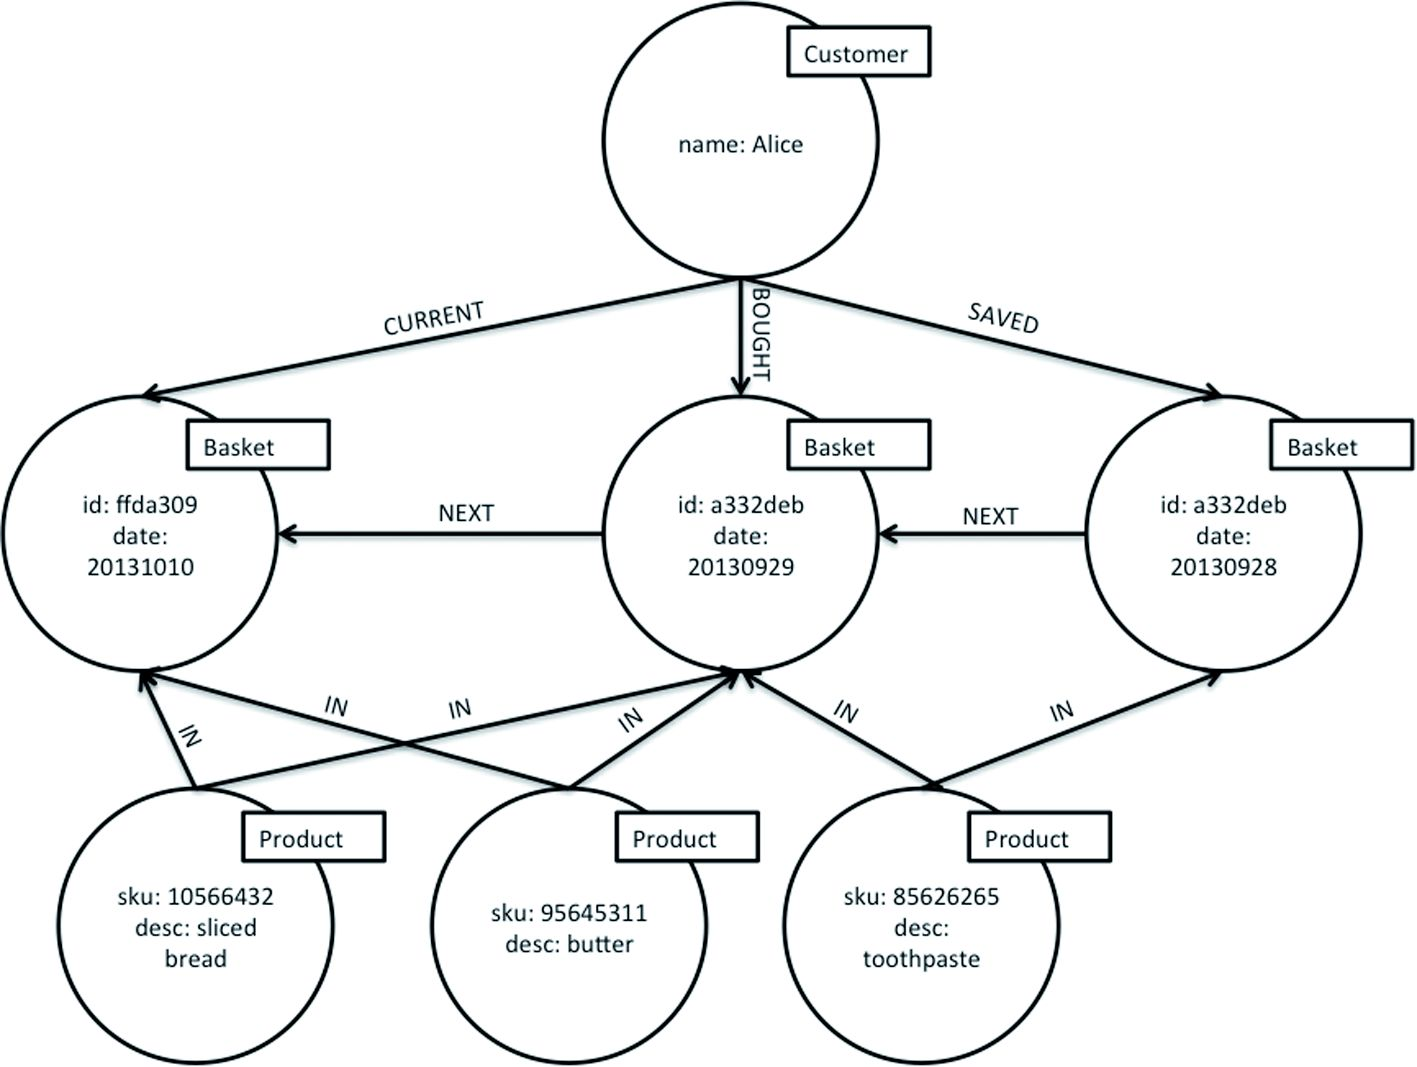
\includegraphics[]{images/graphikdatabase.jpg}
\caption[Graphikdatenbank Beispiel]{Graphikdatenbank Beispiel \protect \footnotemark}
\end{figure}
\footnotetext{\url{https://entwickler.de/online/datenbanken/wunderbare-welt-der-graphen-114728.html}, letzter Zugriff: 9. Februar 2021}

\noindent
\hangindent1cm
\textbf{Dokumentenorientierte Datenbanken:}
Im Kontext der dokumentenorientierte Datenbanken sind Dokumente Objekte mit Eigenschaften, die in einer Sammlung gespeichert werden. 
Während eine Sammlung eine Tabelle im relationalen Datenbank widerspiegelt, ist ein Dokument als ein Eintrag beziehungsweise einer Zeile dieser Tabelle gleichzusetzen, mit dem großen Unterschied, dass dokumentenorientierte Datenbanken schemafrei sind und kein bestimmtes Datenschema voraussetzen. 
Dokumente können weitere Dokumente als Attribut oder in einer Liste einbetten und bieten so die Möglichkeit, komplexe Datenstrukturen zu speichern.  
In aktuellen Datenbanksystemen wie CouchDB und MongoDB nutzen diese Dokumente Datenformate wie JSON oder XML.\\

\begin{lstlisting}
{
	"Vorname": "Max",
	"Nachname": "Mustermann",
	"Telefon-Nr": "0124567",
	"Alter": 33,
	"Adresse": "Musterstrasse 34, MusterStadt",
	"Kinder":  ["Junior","Elenor"]
}
\end{lstlisting}

\noindent
\hangindent1cm
\textbf{Key-Value-Datenbanken:}
Key-Value-Datenbanksysteme bilden mit einer Abbildung der Daten in Schlüssel- und Wertpaare die einfachste NoSQL-Datenbankumsetzung ab. Bei diesem Konzept werden eindeutigen Schlüsselattributen (Key) jeweils ein beliebiger Wert (Value) zugeordnet. %(siehe Tabelle \ref{tab:key_value_db}).

%\begin{table}[tbt]
%\caption{Key-Value Beispiel}
%\begin{center}
%    \begin{tabular}{ l  l }
%	\toprule
%    \textbf{Key} & \textbf{Value} \\
%    \midrule
%    K1 & AAA,BBB,CCC\\
%    
%
%    K2 &  AAA,BBB\\
%
%
%	K3 & AAA,DDD\\
%
%
%    K4 & BBB,2,01/01/2015 \\
%	\bottomrule
%    \end{tabular}
%\end{center}
%\label{tab:key_value_db}
%\end{table}

\noindent
\hangindent1cm
\textbf{Spaltenorientierte Datenbanken:}
Spaltenorientierte Datenbanken, oder auch „Wide-Column“-Datenbanken genannt, speichern ihre Datensätze in Form von Tabellen.  Sie wirken zunächst den Tabellen der relationalen Datenbanksysteme sehr ähnlich, unterscheiden sich grundlegend aber in der Speicherung der Daten, die nicht zeilenorientiert, sondern spaltenorientiert abgelegt werden. 
Die zeilen- und die spaltenorientierte Speicherung ist in Abbildung \ref{fig:spalten_zeilen_speicher} dargestellt. Zeilenorientierung bei der Speicherung bietet vorallem Vorteile bei Abfragen, bei denen Informationen aus mehreren Spalten benötigt werden.
Spaltenorientierung dagegen eignet sich sehr gut für die Auswertung von Aggregaten.
\newline

\begin{figure}[tbt]
	\begin{subfigure}{\textwidth}
		\centering
		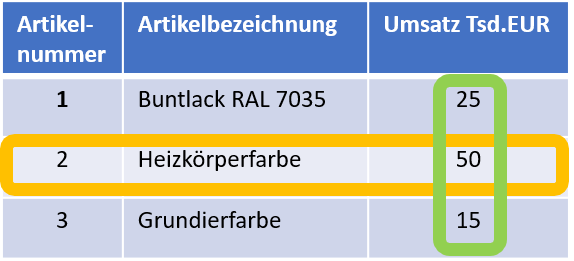
\includegraphics[width=8cm, height = 3cm]{images/SpaltenorientiereDatenbank.png}
		\caption{}
		\label{fig:spalten_zeilen_speicher}
	\end{subfigure}
	\newline
	\begin{subfigure}{\textwidth}
		\centering
		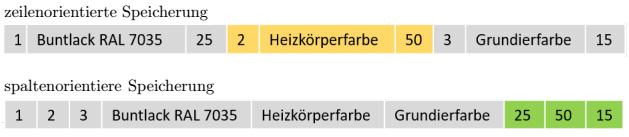
\includegraphics[width=15cm]{images/zeilenspaltenorientiert.png}
		\caption{ }
		\label{fig:spalten_zeilen}
	\end{subfigure}
	\caption[Zeilen- und spaltenorientierte Speicherung]{(a) Spaltenorientierte Datenbank Beispiel (b) Zeilen- und spaltenorientierte Speicherung \protect \footnotemark}
\end{figure}
\footnotetext{\url{https://www.axiom-net.de/die-datenbank-hana-ist-spaltenorientiert}, letzter Zugriff: 9. Februar 2021}

\subsubsection{BASE}
TODO
\newline

\subsubsection{CAP-Theorem}
Der Informatiker Eric Brewer von der Universität Berkeley stellte Anfang des Jahres 2000 die Annahme auf, dass ein System nicht gleichzeitig die drei Kerneigenschaften Consistency (Konsistenz), Availability (Verfügbarkeit) und Partition Tolerance (Ausfalltoleranz) abdecken kann [NoSQL 1.6]. 
\newline

\begin{figure}[tbt]
\centering
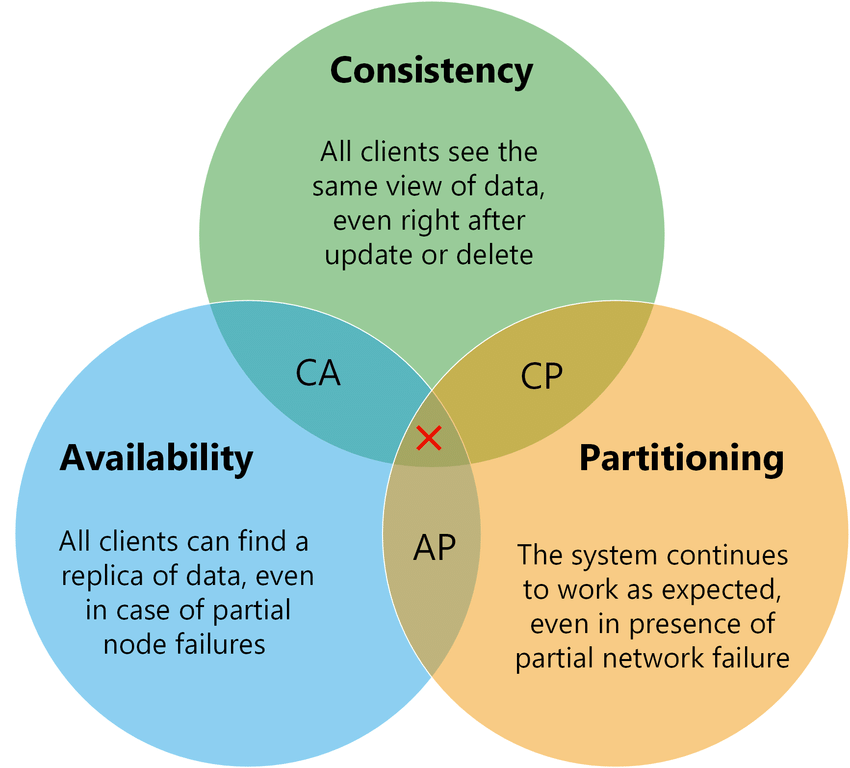
\includegraphics[width=8cm, height=6.5cm]{images/Visualization-of-CAP-theorem.png}
\caption[Visualization-of-CAP-theorem]{Visualization-of-CAP-theorem \protect \footnotemark}
\end{figure}
\footnotetext{\url{https://www.researchgate.net/profile/Hamzeh-Khazaei/publication/282679529/figure/fig2/AS:614316814372880@1523475950595/Visualization-of-CAP-theorem.png}, letzter Zugriff: 10. Februar 2021}

\noindent
Die \textbf{Konsistenz (C)} beschreibt, dass Datenzustände, die in einem verteilten System geändert  werden, in jedem zusammenhängenden System gleich sein müssen. Der Zustand der Daten soll somit im gesamten System übereinstimmen. Ein System, das einen ununterbrochenen Betrieb und eine akzeptable Antwortzeit aufweisen kann, besitzt eine hohe \textbf{Verfügbarkeit (A)}. Die \textbf{Ausfalltoleranz (P)} steht für ein Verhalten, bei dem es bei Ausfallen eines Bestandteiles innerhalb eines Systems  zu keinem Gesamtausfall kommt.

\newpage
\subsubsection{MongoDB}
MongoDB ist ein in C++ geschriebenes, dokumentenorientiertes NoSQL-Datenbanksystem, das im Jahre 2009 von den Entwicklern Horowitz und Merriman als Open-Source Datenbank veröffentlicht wurde und die am weitest-verbreiteste NoSQL-Datenbank (Stand April 2021) \cite{DB1.7}. Die Intention der Gründer war es, eine Datenbank mit höherer Skalierbarkeit, Flexibilät und Performance zu entwerfen, die auf auf einer einfachen Handhabung beruht \cite{DB1.65}.
Gründe der Popularität der Datenbank ist neben den oben erwähnten Eigenschaften die flexible Gestaltungsmöglichkeit der Datenstrukturen sowie die Unterstützung durch zahlreiche Programmiersprachen und Betriebssysteme.
\noindent
Dem Konzept des CAP-Theorems folgend steht MongoDB für Konsistenz und Partitionstoleranz, dafür ordnet sich die Verfügbarkeit den anderen Eigenschaften unter.
\newline

\paragraph{Struktur}

\begin{figure}[tbt]
\centering
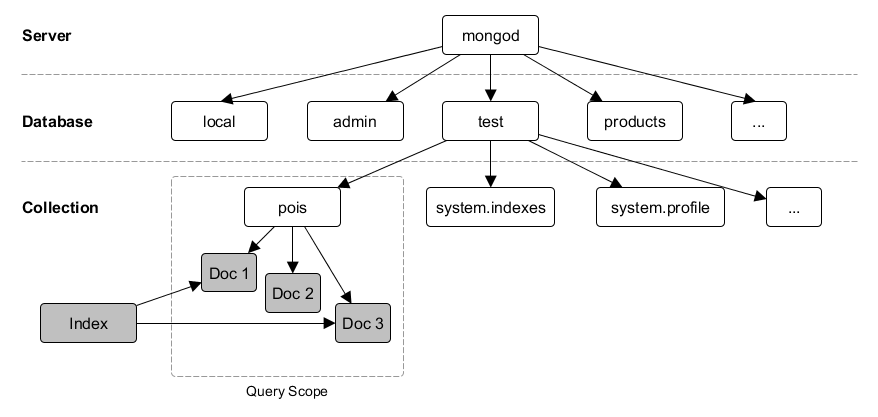
\includegraphics[width=14cm]{images/MongoDB_Architektur.png}
\caption[Graphikdatenbank Beispiel]{Graphikdatenbank Beispiel \protect \footnotemark}
\end{figure}
\footnotetext{\url{https://www.informatik-aktuell.de/betrieb/datenbanken/mongodb-fuer-software-entwickler.html}, letzter Zugriff: 9. Februar 2021}

\noindent
Letztere Abbildung stellt die grundsätzliche Struktur einer Mongo"-DB-"-Instanz dar.
Ein \textbf{Server} kann mehrere logische \textbf{Datenbanken} verwalten, die ihrerseits einen oder mehrere logische Namensräume enthalten, die sogenannten \textbf{Collections}. Eine Collection verwaltet die einzelnen Datensätze, die als \textbf{Dokumente} bekannt sind. 
\newline

\noindent
\subparagraph{Schema-Freiheit}
Collections sind schemafrei. Dadurch gibt es für die zugehörigen Dokumente kein vorausgesetztes Schema. Aufgrund der Schema-Freiheut dürfen dennoch Architekturentscheidungen bei der Datenmodellierung nicht ignoriert werden. Stattdessen werden diese Entscheidungen des Schema-Managements auf die Anwendungsentwicklung verlagert.
\newline

\noindent
\subparagraph{BSON}
Während MongoDB für Datenaustausch das JSON-Format nutzt, hält es seine Dokumente im Binary JSON-Format (BSON), einer binärcodiertem Erweiterung des JSON-Formats. Daten im BSON-Format enthalten zusätzlich Informationen zum Typ und zur Länge der Informationen, wodurch schnelleres Parsen von Daten möglich ist. Des Weiteren ist BSON um zusätzliche Datentypen wie 32- und 64-bit Integer oder das Datum erweitert \footnote{\url{https://www.mongodb.com/json-and-bson]}, letzter Zugriff: 12. Februar 2021}.
\newline

\begin{lstlisting}[caption=JSON - BSON Vergleich, label=lst:JSONBSON]
/* JSON */
{"hello": "world"}  // "key":"value"

/* BSON */
\x16\x00\x00\x00           // Gesamtgroesse des Dokuments
\x02                       // 0x02 = Typ String
hello\x00                  // Feldname
\x06\x00\x00\x00world\x00  // Feldwert
\x00                       // 0x00 = Typ EOO ('end of object')
\end{lstlisting}


\noindent
\subparagraph{ObjectID und Primärschlüssel}
Für die eindeutige Identifikation eines Dokuments vergibt MongoDB automatisch erstellte '\_id\'-Felder. Dabei wird bei der Generierung des BSON-Dokuments für den Wert das '\_id'-Feld ein Datentyp 'ObjectId\'  hinzugefügt. Dieses Identifikationsfeld ist gleichzusetzen mit den Primärschlüsseln aus relationalen Datenbanken \cite{DB1.85}. Ist eine automatische Generierung des eindeutigen Identifikationsfeldes nicht erwünscht, kann der Anwendungsentwickler dieses Feld auch selbst erzeugen, indem er die Eigenschaft explizit dem zu erstellenden Objekt hinzufügt und mit einem Wert verseht.
\newline

\paragraph{Datenbankabfrage}
Im Vergleich zu relationalen Datenbanken benutzt MongoDB keine Abfragesprache wie SQL. Stattdessen ermöglicht dieses Datenbanksystem drei Arten von Abfragen, wobei eine Abfrage sich immer auf genau eine Collection bezieht. Ein Bezug einer Abfrage zu mehreren Collections, wie es relationale Datenbanken mit „Join“-Operationen erlauben, ist hier nicht gegeben und muss in der Anwendung realisiert werden \cite{1.9}. Abfragen in MongoDB werden grundsätzlich in Form von Dokumenten formuliert. Dieses Verfahren ermöglicht schnelles Abhandeln komplexer Abfragen von tief geschachtelten Dokumentenstrukturen. Nachfolgend werden die drei Abfragemöglichkeiten erläutert.

\noindent
\subparagraph{Query-By-Example}
Das folgende Beispiel zeigt einen Aufruf aller Einträge, die als Ort Karlsruhe eingespeichert haben. 
\newline
\begin{lstlisting}[caption=MongoDB Read, label=lst:MongoDBRead]
db.pois.find( {"adresse.ort": "Karlsruhe" } )
\end{lstlisting}

\noindent
Dabei kommt das Prinzip Query-by-Example \footnote{Query By Example: \url{https://de.wikipedia.org/wiki/Query_by_Example}, letzter Zugriff: 12. Februar 2021} zum Einsatz, bei dem die als JSON-Dokument beschriebenen Suchkriterien als Filter auf die durchsuchte Collection wirkt. Zusätzlich stehen für diese Art von Abfragemöglichkeit sämtliche logische Verknüpfungen und Vergleichsoperatoren zur Verfügung\footnote{Query-Operatoren\url{https://docs.mongodb.com/manual/reference/operator/query/}, letzter Zugriff: 12. Februar 2021}.
Das Ergebnis der obigen Find-"-Operationen liefert dabei einen Cursor zurück, über den die aufrufende Anwendung durch die einzelnen zurückgelieferten Dokumente iterieren kann. Außerdem kann der Cursor modifiziert werden, um beispielsweise Beschränkungen der Trefferanzahl oder Sortierung vorzunehmen.
\newline
\begin{lstlisting}[caption=MongoDB Read Modifikation, label=lst:MongoDBReadModifikation]
db.pois.find().limit(5).sort({"adresse.ort": -1})
\end{lstlisting}

\noindent
\subparagraph{MapReduce}
MapReduce ist ein allgmeines Programmiermodell zur verteilten und parallelen Verarbeitung von großen Datenmengen in aggregierte Ergebnisse. Dabei unterteilt sich der Algorithmus im Wesentlichen in zwei Operationen \footnote{MapReduce Dokumentation \url{https://docs.mongodb.com/manual/core/map-reduce/}, letzter Zugriff: 10. Februar 2021}
\newline
-	Map: Emittieren der beliebig vielen Key-Value-Paare für jedes Dokument
\newline
-	Reduce: Zusammenfassen aller Daten, die einem Kriterium entsprechen.

\noindent
\subparagraph{Aggregation-Framework}
Das Aggregation-Framework bietet als Alternative zum MapReduce-Verfahren den Vorteil der besseren Performance\footnote{\url{https://docs.mongodb.com/manual/meta/aggregation-quick-reference/}, letzter Zugriff: 14. Februar 2021}. Dabei wird eine Pipeline genutzt, die das resultierende Dokument einer Operation an die Eingabe der nächsten Operation weiterleitet. Die entsprechende Funktion ist die Aggregate()-Operation, deren Parameter als Array von Dokumenten die Pipeline-Operatoren abbilden .
\newline 

\begin{lstlisting}[caption=MongoDB Aggregate, label=lst:MongoDBAggregate]
db.pois.aggregate([
    {$group: {_id: "$adresse.ort", n: {$sum:1}}},
    {$sort: {n: -1}}
])
\end{lstlisting}


Es stehen folgende Pipeline-Operatoren zur Verfügung:

 

\begin{table}[tbt]
\caption[Aggregation Framework: Pipeline-Operatoren]{Aggregation Framework: Pipeline-Operatoren [MongoDB1.9]}
\begin{center}
    \begin{tabular}{ l  p{12cm}}
    \toprule
    \textbf{Operator}  & \textbf{Beschreibung} \\
    \midrule
\rule{0pt}{17pt}
    \$match &Sucht Dokumente analog zu find(). Sollte idealerweise mindesten 1x zu Beginn der Pipeline ausgeführt werden, um die Ergebnismenge einzuschränken.\\
    
\rule{0pt}{17pt}
    \$project & Schränkt auf eine Teilmenge von Feldern ein und verändert die Feldwerte.  \\
    
\rule{0pt}{17pt}
	\$sort & Sortiert die Dokumente. Analog zu sort() bei find(). .\newline
	Benötigt Private Key und Zertifikat.  \\
	
\rule{0pt}{17pt}
    \$skip & Überspringt n Dokumente. Analog zu skip() bei find().  \\ 
    
\rule{0pt}{17pt}
    \$limit & Begrenzt auf n Dokumente. Analog zu limit() bei find().  \\

\rule{0pt}{17pt}
   \$group   &	Gruppiert nach einem oder mehreren Feldern. \\ 

\rule{0pt}{17pt}
	\$unwind  &	Wird auf ein Array angewendet. Jeder Array-Eintrag generiert dann ein neues Dokument für die nächste Pipeline-Stufe.\\

\rule{0pt}{17pt}
	\$redact  &	Filtert Felder des Dokuments in Abhängigkeit vom Inhalte anderer Felder.\\

\rule{0pt}{17pt}
	\$out  &	Leitet das Ergebnis der Aggregation in eine Collection um. Kann nur als letzter Operator verwendet werden.  \\
    \bottomrule
    \end{tabular}
\end{center}
\caption[Aggregation Framework: Pipeline-Operatoren]{Aggregation Framework: Pipeline-Operatoren \protect \footnotemark}
\end{table}
\footnotetext{\url{https://www.informatik-aktuell.de/betrieb/datenbanken/mongodb-fuer-software-entwickler.html}, letzter Zugriff: 9. Februar2021}



\paragraph{CRUD} TODO TABLE :(
MongoDB unterstützt eine Vielzahl an Operationen zum Erzeugen, Lesen, Updaten und Löschen von Daten.
Über folgende Kommandos lassen sich die CRUD-Operationen realisieren:
\newline

\begin{table}[tbt]
\caption{CRUD-Operatoren}
\begin{center}
    \begin{tabular}{ l  p{8cm}  l }
    \toprule
    \textbf{Operation} & \textbf{Beschreibung} & \textbf{MongoDB Methode} \\
    \midrule

    Create & Datensätze erstellen & .Insert() \\

	Read & Datensätze lesen & .Find() \\

    Update & Daten aktualisieren & .Update() \\ 

    Delete & Datensätze entfernen & .Remove()  \\ 
    \bottomrule
    \end{tabular}
\end{center}
\end{table}

\noindent
\hangindent1cm
\textbf{Create:}
„InsertOne()“ erzeugt ein einzelnes Dokument in der jeweiligen Collection der Datenbank. Dabei wird ein Dokument im JSON-Format als Parameter mitgegeben. ObjectID wird, wenn nicht als Eigenschaft im Dokument angegeben, automatisch von MongoDB erzeugt. Ebenfalls wird die angesprochene Collection automatisch erzeugt, falls sie nicht bereits existiert. Die Funktion „InsertMany()“  erlaubt das Hinzufügen mehrerer Datensätze über ein Array von JSON-Dokumenten als Parameter. Die Methode „Insert“ ist flexibler und bietet beide Parametrisierungsmöglichkeiten\footnote{\url{https://docs.mongodb.com/manual/reference/method/db.collection.insert/\#mongodb-method-db.collection.insert}, letzter Zugriff: 14. Februar 2021}.
\newline
\begin{lstlisting}[caption=MongoDB Create, label=lst:MongoDBCreate]
db.personen.insertOne({"vorname" : "Robin"});
\end{lstlisting}

\noindent
\hangindent1cm
\textbf{Read:}
Um Datensätze aus der Datenbank zu lesen, wird die find()-Methode zur Verfügung gestellt. Sie gibt alle Dokumente einer Kollektion zurück. Wie im Kapitel Query-By-Example beschrieben, kann die Funktion mit Filtern versehen werden. Die Funktion findOne() bietet die gleiche Funktionsweise, die Dokumentenausgabe ist aber auf ein einzelnes Dokument begrenzt. 
Ein Beispiel ist dargestellt in Listing \ref{lst:MongoDBRead}.
\newline\newline

\noindent
\hangindent1cm
\textbf{Update:}
Die Update()-Methode ermöglicht es, Änderungen an Datensätzen vorzunehmen.  Die Methode erhält zwei Parameter, einen zur Angabe der gesuchten Dokumente und den anderen mit  der vorzunehmenden Änderung. Simultan zu den Insert-Methoden gibt es die UpdateOne()-Methode für Änderungen an einem Dokument und UpdateMany()-Methode für mehrere Dokumente.
\newline

\begin{lstlisting}[caption=MongoDB Update, label=lst:MongoDBUpdate]
db.personen.updateOne({"vorname" : "Robin"} , currentDate("last_login") );

\end{lstlisting}

\noindent
\hangindent1cm
\textbf{Delete:}
Für das Löschen von Datensätzen aus einer Collection gibt es die DeleteOne()- und DeleteMany()-Methode. Über mitgegegeben Parameter können Filter eingestellt werden. Eine ganze Collection kann mit der drop()-Methode entfernt werden.
\newline

\begin{lstlisting}[caption=MongoDB Remove, label=lst:MongoDBRemove]
db.personen.deleteOne( {"vorname" : "Robin"} );

\end{lstlisting}

\noindent
\paragraph{Atomare Operationen}
Als atomare Operationen wird ein Verbund von Einzeloperationen bezeichnet, der als logische Einheit betrachtet wird und nur als Ganzes erfolgreich abläuft oder fehlschlägt. In Bezug auf Datenbanken spricht man von Transaktionen, die entweder als Ganzes erfolgreich ablaufen (Commit) oder nach einer fehlerhaften Einzeloperation rückgangig gemacht werden (Rollback). Ohne atomare Operationen können Probleme aufkommen, die zu einer Inkonsistenz der Datenzustände führt. Beispielsweise würde ein Abbruch inmitten mehrerer zusammenhängender Operationsabläufe dazu führen,  dass nur ein Teil der Operationen ausgeführt wurde, während die restlichen Operationen und somit die verbleibenden Datenänderungen verworfen werden.
\newline
Bis vor dem Jahre 2018 unterstützte MongoDB keine Transaktionen. Mit der Veröffentlichung der Version 4.0 wurde der Funktionsumfang von MongoDB stark erweitert. Eines der neuen Erweiterungen war die Möglichkeit, Transaktionen durchführen zu können. Dafür werden sogenannte „Sessions“ genutzt. Sämtlichen CRUD-Operationen, die einer Transaktion zugehören sollen, werden eine Session als zusätzlicher Parameter hinzugefügt.  Bei Abschluss der Transaktion kann sie mit der Methode „session.commitTransaction()“ bestätigt werden. Andernfalls, sollte ein Fehler aufgetreten sein, kann die Methode „session.abortTransaction()“ die Operationen rückgängig machen. Eine wichtige Vorraussetzung, um Transaktionen in MongoDB nutzen zu können, ist ein Replica Set aufzusetzen. Darauf wird im weiteren Kapitel eingegangen. 
\newline


\paragraph{Architektur}
Bei der Inbetriebnahme einer MongoDB Datenbank spielen zwei Prozesse eine wichtige  Rolle. \newline Der  „mongod“-Prozess ist der primäre Hintergrundprozess für das Datenbanksystem. Er behandelt Datenabfragen, Datenzugriffe und führt benötigte Hintergrundoperationen durch\footnote{Mongod \url{https://docs.mongodb.com/manual/reference/program/mongod/}, letzter Zugriff: 15. Februar 2021}. Beim Starten des mongod-Prozesses können über Flags Konfigurationen vorgenommen werden, beispielsweise ändert „--port 5000“ den Port. Nach erfolgreichem Start des Prozesses kann über den Standard Port der MongoDB (27017) bzw. über den konfigurierten Port eine Verbindung hergestellt werden.\newline
Der Prozess, der als Controller für sich auf mehreren Datenbanken befindenden verteilte Daten dient, nennt sich „mongos“\footnote{Mongos \url{https://docs.mongodb.com/manual/reference/program/mongos/}, letzter Zugriff: 15. Februar 2021}. Dieser Prozess findet seinen Einsatz hauptsächlich in Kombination mit Sharding, auf die im weiteren Unterkapitel eingegangen wird. \newline

\noindent
\hangindent1cm
\textbf{Engine:}
Als Storage Engine, oder auch Datenbank-Engine, wird die zugrundeliegende Softwarekomponente eines Datenbanksystems zum Verwalten der Daten bezeichnet. Die gebräuch"-lich"-sten Engines in MongoDB sind die MMAPv1-Engine und die WiredTiger-Engine.\newline
Bis vor Version 3.2 war MMAPv1-Engine die Standard-Storage Engine von MongoDB. Eine Kompression der Daten wurde nicht unterstützt und Transaktionen waren nur auf einem Dokument ausführbar. Ab MongoDB 3.2 wird standardmäßig die Wired Tiger-Engine eingesetzt. Neben der Kompression der Daten und der miteingehenden Verringerung des benötigten Speicherplatzes bietet diese Engine auch eine Verschlüsselung der Daten an. Abhängig des benutzten Kompressionsalgorithmus kann der benötigte Verbrauch um 70\% für Daten und um 50\% für Indizes reduziert werden \cite{DB3.5}. Die WiredTiger-Engine skaliert im Vergleich zur MMAPv1 mit der Anzahl der CPU-Kerne und ermöglicht Transaktionen über mehrere Dokumente hinweg. Die genutzte Engine kann in den Konfigurationen eingestellt werden.
\newline

\noindent
\hangindent1cm
\textbf{Replica Sets:}
Im standardmäßgen Standalone-Modus besteht bei Ausfall des Servers die potenzielle Gefahr des Datenverlusts. Das Problem lässt sich durch Replikation beheben. Hierbei spricht man von der bloßen Herstellung von Mehrexemplaren(Kopien) derselben Daten, die meistens regelmäßig abgeglichen werden \cite{DB3.6}. MongoDB realisiert die Replikation der Daten über Replica Sets\cite{DB3.7}. Dabei handelt es sich um eine Gruppe von mongod-Prozessen, die dieselben Daten enthalten. Nach dem CAP-Theorem ist MongoDB nicht auf Verfügbarkeit ausgelegt. Dennoch umgeht die Datenbank diesen Nachteil über die Anwendung von Replica Sets. Das Replica Set besteht aus einem primären Knoten und daraus replizierenden Sekundären Knoten.
Nur der primäre Knoten führt datensatzändernde Operationen aus. Veränderungen werden in sogenannten 'Oplogs' (Operations logs) gespeichert, die zum Austausch der Daten innerhalb des Replica Sets genutzt wird \cite{DB3.8}. Bei den Oplog-Dateien handelt es sich um Collections mit festgelegten Speichergrößen, den sogenannten „capped collections“. Während die Oplog-Dateien ähnlich wie ein Logbuch mit allen Veränderungen in den Datensätzen der Datenbank beschrieben werden, werden bei erreichter Maximalgröße der Collection die ältesten Daten von den neuen Daten überschrieben. Dabei enthält jeder Knoten des Replica Sets seine eigene Kopie des Oplogs und gleicht ihn mit dem des primären Knotens ab.

\begin{figure}[tbt]
\centering
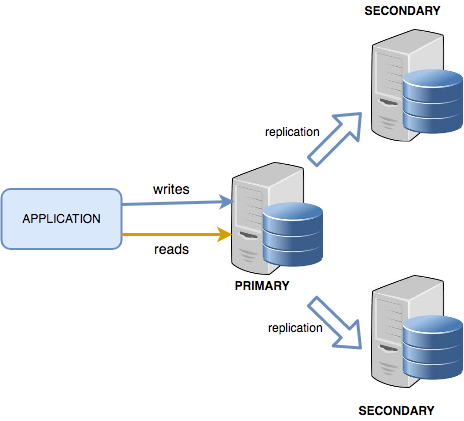
\includegraphics[width=7cm]{images/replicaset1.png}
\caption{MongoDB Replica Set}
\end{figure}
\footnotetext{Bild aus \cite{DB3.8}}


\noindent
\hangindent1cm
\textbf{Sharding:}
Hierbei ist die Rede von der Methodik zur Aufteilung der Daten auf mehrere Datenbanken \cite{DB4.1}.
Der Datenbestand wird nach logischen Kriterien in  Teilstücke, die sogenannten „Shards“, zerlegt und über mehrere Replica Sets verteilt.
In Hinblick auf das hinzufügen weiterer Server gewährt das Sharding eine horizontale Skalierbarkeit.
Des Weiteren werden durch die Tatsache, dass jeder Shard für seinen Bestandteil zuständig ist,  Suchanfragen schneller durchgeführt. 
Sharding ist besonders bei großen Datenmengen in Bezug auf Performance von Vorteil.
Der mongos-Prozess leitet Anfragen an die jeweiligen Shards weiter und dient als Schnittstelle zwischen den Clientanwendungen.

\paragraph{Verwaltungswerkzeuge}
\noindent
\hangindent1cm
\textbf{Mongo Shell:}
Der „mongo“-Prozess ist eine interaktive JavaScript Schnittstelle auf der Kommandozeile. Er bietet umfassende Funktionalitäten für die Systemadministration des Datenbankensystems als auch Zugriff auf die Datensätze\footnote{Mongo \url{https://docs.mongodb.com/manual/reference/program/mongo/}, letzter Zugriff: 15. Februar 2021}. Dazu erhält man eine Eingabeaufforderung, auf dem Befehle in der Sprache JavaScript ausgeführt werden können.
\noindent
\hangindent1cm
\textbf{Treiber:}
MongoDB bietet für viele Programmiersprachen bzw. Frameworks Softwarebibliotheken zum Zugriff auf die Datenbank an.\footnote{MongoDB Treiber \url{https://docs.mongodb.com/drivers/}, letzter Zugriff: 01. Mai 2021}  Eine offiziell unterstützte ist Mongoose für das Node.js-Framework\footnote{Mongoose - Offizielle Webpage \url{https://mongoosejs.com/docs/}, letzter Zugriff: 01. Mai 2021}
\newpage
\noindent
\hangindent1cm
\textbf{Grafische Oberflächen:}
Es gibt einige Anwendungen zur visuellen Darstellung und Bearbeitung der Datenbanken in MongoDB, die eine grafische Benutzeroberfläche bieten. Zum Beispiel MongoDB Compass, Studio3T oder Fang of Mongo. 


\begin{figure}[tbt]
\centering
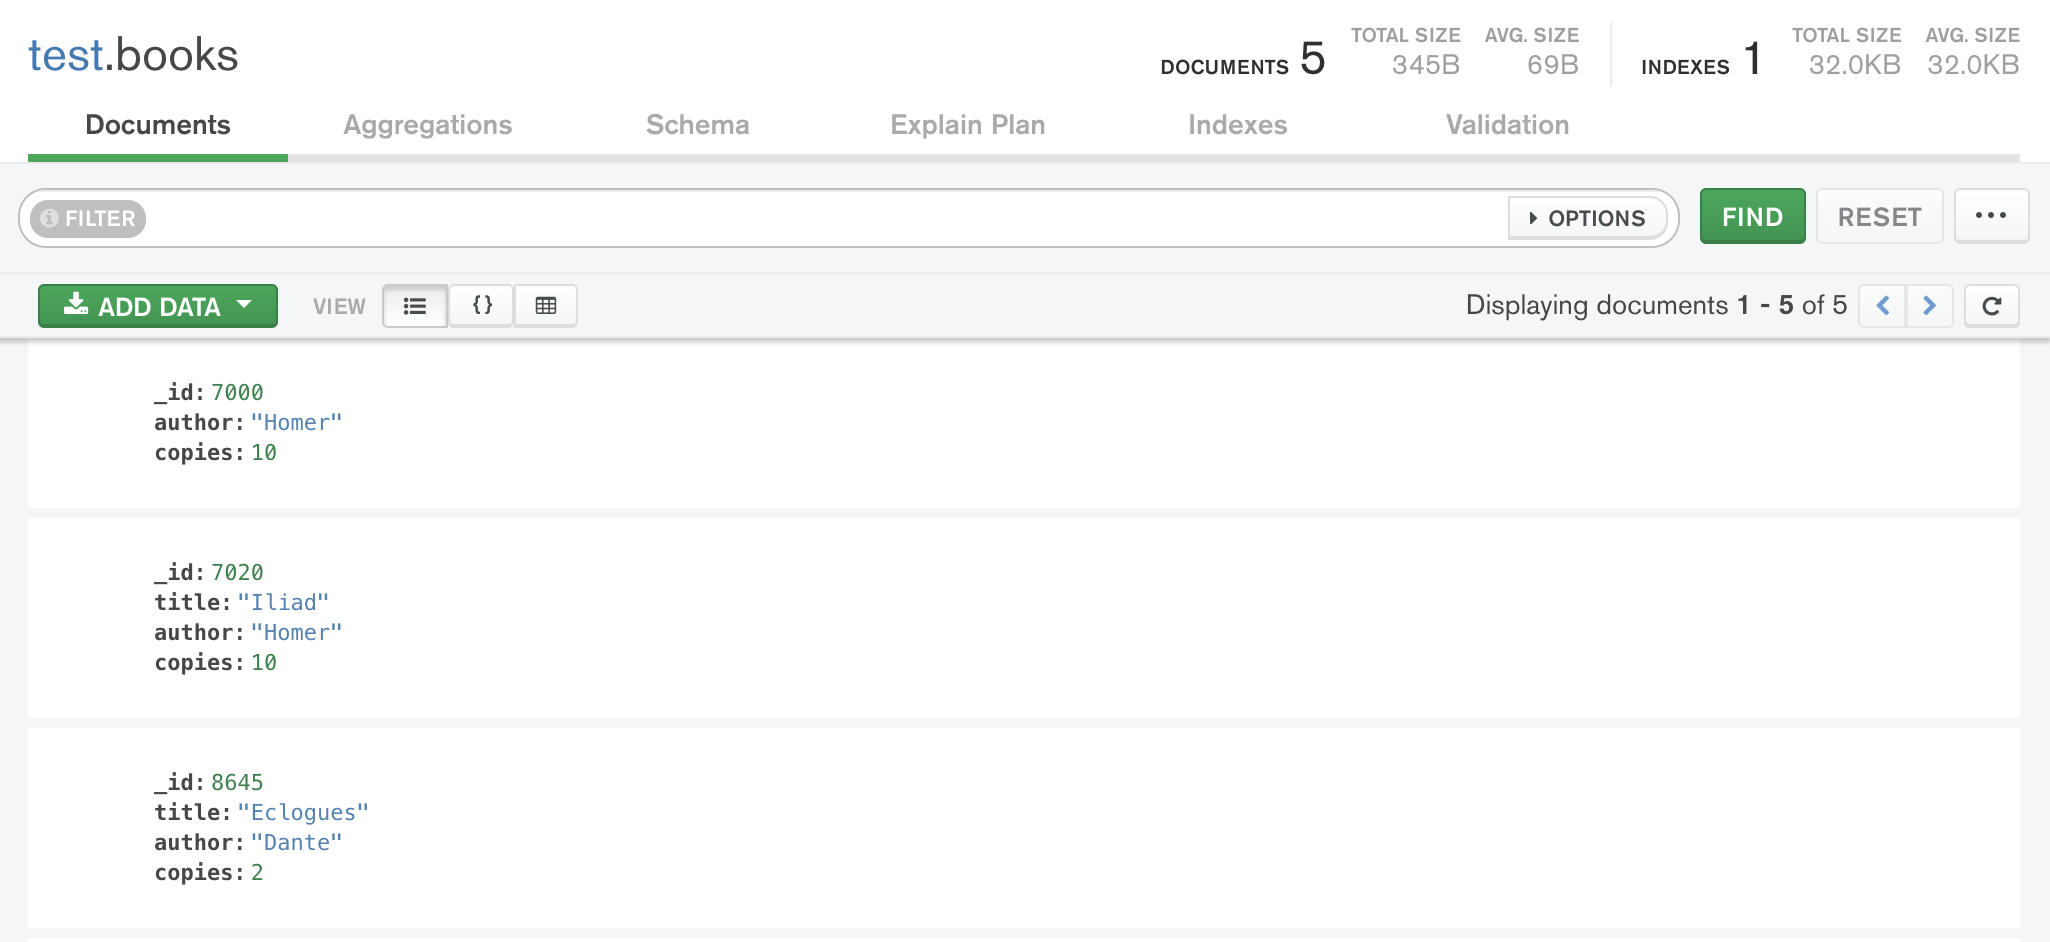
\includegraphics[width=15cm]{images/mongodb_compass.png}
\caption{CRUD-Besipielfunktionen eines Mongoose-Models}
\end{figure}
\subsection{Firebase}
\label{sec:firebase}
Firebase ist eine Backend as a Service-Plattform (BaaS)  von Google für mobile und Web-Anwendungen. 
Sie soll es dem Entwickler ermöglichen, einfacher und effizienter Funktionen auf verschiedenen Plattformen bereitzustellen stellt Tools und Infrastruktur zur Verfügung.
Mit dem Firebase SDK bietet die Plattform API Schnittstellen zu den jeweiligen Tools, welche direkt in die Anwendung integriert werden können, ohne dass serverseitiger Code dafür notwendig ist.
Die Firebase Inc. wurde 2011 von James Tamplin und Andrew Lee gegründet und letztendlich 2014 von Google übernommen.\footnote{\href{https://firebase.googleblog.com/2014/10/firebase-is-joining-google.html}{firebase.googleblog.com}, zuletzt aufgerufen am 03.05.2021}
Teile der SDK stehen seit der Google I/O 2017 unter der Apache 2.0 Lizenz, sind somit also Open-Source.\footnote{\href{https://opensource.googleblog.com/2017/05/open-sourcing-firebase-sdks.html}{opensource.googleblog.com}, zuletzt aufgerufen am 03.05.2021}\\
\\
Es existieren zwei Kostenmodelle für die Nutzung von Firebase: Ein kostenloses Modell \glqq Spark Plan\grqq und ein pay-as-you-go \glqq Blaze Plan\grqq . Das kostenlosen Modell beinhaltet die wichtigsten Tools, viele dieser Tools sind jedoch begrenzt durch beispielsweise Bandbreite oder Speicherplatz.
Der Pay-as-you-go Plan ist eine Erweiterung des kostenlosen Plans. 
Er bietet daher das Nutzen von Tools bis zu einem gewissen Limit kostenfrei an; darüber hinaus kostet es jedoch dann pro Nutzung.\\
\\
Ein Firebase Projekt ist die oberste Ebene in Firebase. 
Ein Projekt ist letztendlich ein \textit{Google Cloud Projekt}, welches mit speziellen Konfigurationsmöglichkeiten und Services ausgestattet ist. 
Es beinhaltet die Verknüpfung zu den einzelnen Anwendungen (also bspw. Android-, iOS- oder Webanwendung). Nun können variabel Tools, sog. Firebase products hinzugefügt werden. Diese Produkte lassen sich grundlegend in drei Kategorien einteilen. Die hier relevantesten werden im Folgenden besprochen.\cite{firebase2021}

\subsubsection{Firebase Authentifizierung}
Die Authentifizierung gehört zu den \glqq Build\grqq Produkten und bietet eine Token-basierte Nutzerauthentifizierung. 
Hierbei kann zwischen verschiedenen Anmeldeoptionen gewählt werden: klassisch mit E-Mail und Passwort, mit OAuth2.0 Integration für Social Media (Google, Facebook, Twitter, Github, ...) oder per Telefonnummer.
Jeder Nutzer erhält eine einzigartige ID und ein zugehöriges Nutzerobjekt in einer NoSQL Datenbank. Grundlegende Werte wie E-Mail Adresse oder Name können hier abgespeichert werden; zusätzliche Informationen müssen über einen weiteren Datenbank Service abgespeichert werden.
Für die Verwaltung eines Accounts bietet dieses Tool auch eingebaute E-Mail Aktionen an - bspw. Passwort zurücksetzen oder E-Mail Adresse bestätigen.\\
\\
Ein Firebase Nutzer Objekt repräsentiert den Account eines Nutzers, welcher sich von einer Anwendung aus beim zentralen Firebase Projekt angemeldet hat.
Die Instanz eines Firebase Nutzers ist somit unabhängig von der Authentifizierungsinstanz der Anwendung, also kann eine Anwendung mehrere Nutzer anmelden, jedoch kann sich auch ein Nutzer auf mehreren Anwendungen anmelden.
Ist ein Nutzer authentifiziert, erhält die Anwendung eine Referenz des Nutzers, welche so lange existiert, bis er wieder abgemeldet ist.\cite{firebase2021}

\subsubsection{Cloud Firestore}
\label{sec:firestore}
Als Datenbank Lösung bietet Firebase zwei unterschiedliche Produkte an: Cloud Firestore und Realtime Database.
Firestore ist hier neuer, jedoch ersetzt es Realtime Database nicht. \\
Cloud Firestore ist eine flexible und auf Skalierung ausgesetzte NoSQL Cloud Datenbank, welche unter anderem die Echtzeitsynchronisierung der Daten zwischen Anwendung und Server ermöglicht.
Zusätzlich zu REST und RPC APIs in iOS, Android und web SDKs ist Firestore auch in nativen Node.js, Java, Python und Go SDKs verfügbar.\\
\\

\begin{wrapfigure}{R}{0.4\textwidth}
	\begin{center}
		
\includegraphics[width=0.35\textwidth]{./Theoretische_Grundlagen/images/firestore_datastucture.png}
	\end{center}
	\caption{Datenmodell in Firebase \protect \footnotemark}
	\label{fig:firestore_data_structure}
\end{wrapfigure}
\footnotetext{Quelle: \cite{firebase2021}}

\noindent
Das Datenmodell ist hierarchisch aufgebaut, wobei Daten in Dokumenten (documents) und Dokumente in Sammlungen (collections) gespeichert sind. 
Mithilfe von Sammlungen werden die Daten voneinander abgetrennt und hierüber können Abfragen erstellt werden.
Grundlegende Datentypen sind String, Integer und Boolean, jedoch können auch komplexe Datentypen wie Maps, Arrays oder Geopoints. Unter-Sammlungen und darin verstaute Dokumente sind ebenfalls möglich.\\
\\
Abfragen werden auf Dokumentenebene erstellt, damit nicht eine gesamte Sammlung aufgerufen werden muss.
Dies kann über direkte Sortierung, Filter und/oder Limitierung bzw. genaue Auswahl eines Dokumentes bewerkstelligt werden.
Bei einer Abfrage erhält man einen \textit{Data Snapshot}, wodurch über Änderungen in Echtzeit informiert und diese angezeigt werden können.
Damit es jedoch zu keinen fehlerhaften Daten führt, gelten hier atomare Eigenschaften für Transaktionen.
Eine Transaktion ist eine Folge von Datenbankanweisungen, welche entweder alle gemeinsam oder gar nicht ausgeführt werden. 
Eine Transaktion ist nur dann erfolgreich, wenn alle Anweisungen auf eine Datenbank vollständig geschlossen sind. 
Ist dies nicht der Fall, werden alle Anweisungen bis zum Stand vor der Transaktion rückgängig gemacht. Das nennt man Rollback.\\
\\
Die Sicherheit der Daten stellt Cloud Firestore für Mobil- und Webclient-Bibliotheken über die Firestore-Sicherheitsregeln her. Diese bieten sowohl Zugriffsverwaltung und -authentifizierung, jedoch könne auch Daten hiermit für die Konsistenz der Datenbank validiert werden. 
\medskip
\begin{lstlisting}[caption=Beschränkung des Zugriffs auf Dokumente der Sammlung \texttt{cities}, label=lst:firestorerules_basic]
	service cloud.firestore {
		match /databases/{database}/documents {
			match /cities/{city} {
				allow read, write: if request.auth != null;
			}
		}
	}
\end{lstlisting}
\medskip
Im Beispiel \ref{lst:firestorerules_basic} wird der Lese- und Schreibzugriff auf ein Dokument der Sammlung \texttt{cities} beschränkt. 
Nur falls der anfragende Nutzer eine valide Authentifizierung besitzt, erhält er Zugriff auf das angefragte Dokument. 
Diese simple Darstellung ist jedoch für den wirklichen Produktionseinsatz mit Vorsicht zu nutzen. 
Oftmals müssen \texttt{read} und \texttt{write} in detailliertere Vorgänge aufgeteilt werden. Ein \texttt{read} wird spezialisiert in \texttt{get} und \texttt{list}, wobei ein \texttt{write} in \texttt{create}, \texttt{update} und \texttt{delete} unterteilt werden kann.
Ein \texttt{list} ermöglicht es hierbei auf Sammlungen, also die einzelnen Dokumenten IDs lesend zuzugreifen, jedoch nicht auf die Daten einzelner Dokumente. Hierfür wird dann ein \texttt{get} benötigt. 
Mittels \texttt{create} erhält man Schreibzugriff auf nicht existierende Dokumente, durch \texttt{update} auf bereits vorhandene und Löschrechte ganzer Dokumente erhält man über den \texttt{delete} Operator.\\
\\
Sicherheitsregeln werden gleich dem Datenmodell hierarchisch aufgebaut und ermöglichen differenzierte Zugriffsbeschränkungen auf jeder Ebene.
In Codebeispiel \ref{lst:firestorerules_hierarchy} beinhaltet jedes Dokument (Stadt) der Sammlung \texttt{cities} eine Unter-Sammlung \texttt{landmarks}. Nun lässt sich der Zugriff auf beide separat regeln.
Bei der Sammlung \texttt{villages} hingegen wurde der rekursive Platzhalter verwendet. Hiermit sind Zugriffsregeln auf allen tieferen Ebenen gleich.
Beim Verschachteln von \texttt{match} ist der innere Pfad immer relativ zum äußeren.

Wichtig zu wissen ist hierzu noch, dass falls mehrere \texttt{allow} Ausdrücke auf eine Anfrage zutreffen, wird der Zugriff erlaubt sobald \textbf{eine} Bedingung wahr, also erfüllt ist.

\medskip
\begin{lstlisting}[caption=Hierarchische Zugriffsbeschränkung, label=lst:firestorerules_hierarchy]
	service cloud.firestore {
		match /databases/{database}/documents {
			match /cities/{city} {
				allow read, write: if <condition>;
				
				// Explicitly define rules for the 'landmarks' subcollection
				match /landmarks/{landmark} {
					allow read, write: if <condition>;
				}
			}
			match /villages/{document=**} {
				allow read, write: if <condition>;
			}
		}
	}
\end{lstlisting}
\medskip

\noindent
Wie bereits oben besprochen können diese Regeln auch zur Validierung von Daten genutzt werden, damit die atomare Eigenschaft von Transaktionen bestehen bleibt.
Hierzu kann die \texttt{getAfter()} Funktion genutzt werden. 
Mit dieser kann man auf Zustand eines Dokumentes zugreifen und diesen validieren, nachdem einer Folge von Anweisungen ausgeführt, jedoch diese noch nicht auf der Firestore Datenbank abgeschlossen wurde.
Im Beispiel \ref{lst:firestorerules_validation} existieren zwei Sammlungen: \texttt{cities} und \texttt{countries}. 
Jedes \texttt{country} Dokument beinhaltet das Feld \texttt{last\_updated} um zu wissen, welche Stadt innerhalb eines Landes zuletzt aktualisiert wurde.
Hierzu wird in den Sicherheitsregeln nach jedem Schreibzugriff auf ein \texttt{city} Dokument gleichzeitig auch das Feld des zugehörigen Landes aktualisiert.\cite{firebase2021}
\medskip
\begin{lstlisting}[caption=Datenvalidierung für atomare Operationen, label=lst:firestorerules_validation]
	service cloud.firestore {
		match /databases/{database}/documents {
			// If you update a city doc, you must also
			// update the related country's last_updated field.
			match /cities/{city} {
				allow write: if request.auth != null &&
				getAfter(
				/databases/$(database)/documents/countries/$(request.resource.data.country)
				).data.last_updated == request.time;
			}
			
			match /countries/{country} {
				allow write: if request.auth != null;
			}
		}
	}
\end{lstlisting}
\medskip

\subsubsection{Cloud Storage}
\label{sec:firebase_storage}
Um Filme, Videos oder andere Nutzer-generierte Inhalte abspeichern zu können, bietet Firebase Cloud Storage an. 
Durch das Firebase SDK für Cloud Storage können Dateien direkt von Client-Anwendungen hoch- bzw. heruntergeladen werden.
Aufgrund von möglicher schlechter Verbindung kann mithilfe von robusten Operationen der Prozess des Hoch- bzw. Herunterladens bei besserer Verbindung an der Stelle weiter geladen werden, an welcher dieser unterbrochen wurde.
Ähnlich wie bei Cloud Firestore in Kapitel \ref{sec:firestore} bestimmen auch hier Sicherheitsregeln den Zugriff auf bestimmte Dokumente.\\
Zusätzlich hierzu sind weitere Metadaten verfügbar: \texttt{contentType} und \texttt{size}. 
Mit ihnen lassen sich die Dateien beispielsweise validieren.
Im Code \ref{lst:storagerules_validation} können Dateien nur hochgeladen werden, falls sie eine Größe kleiner 5 MB besitzen.
\medskip
\begin{lstlisting}[caption=Validierung nach Dateigröße, label=lst:storagerules_validation]
	service firebase.storage {
		match /b/{bucket}/o {
			match /images/{imageId} {
				allow read, write: if request.resource.size < 5 * 1024 * 1024
				&& request.auth != null;
			}
		}
		
\end{lstlisting}
\medskip
Außerdem lassen sich durch Cloud Functions aus dem nächsten Kapitel Prozesse automatisieren. Beispielsweise lässt sich beim Upload eines Bildes direkt ein individuelles Thumbnail erstellen lassen.\cite{firebase2021}
\subsubsection{Cloud Functions}
\label{sec:cloudfunctions}
Da Firebase - bis auf vereinfachte Sicherheitsregeln - eigentlich keinen Backend Code benötigt, jedoch manche Features eben genau diesen brauchen, um beispielsweise Benachrichtigungen an Nutzer zu senden oder Bilder zu komprimieren, existieren Cloud Functions.\\
Diese ermöglichen es, als Antwort auf ein Event automatisch oder durch HTTPS Anfrage manuell Backend Code auszuführen.
Der gesamte Code ist hierbei in der Google Cloud gespeichert und wird in einer verwalteten Umgebung ausgeführt.
Als Programmiersprache kann sowohl JavaScript als auch Typescript verwendet werden.\\
\\
\glqq Google Cloud Functions ist die serverlose Computerlösung von Google zum erStellen ereignisgesteuerter Anwendungen.\grqq \cite{firebase2021} 
Es kann sowohl auf der Google Cloud Platform (GCP) also auch für Firebase genutzt werden. 
Es ist bei beiden ein Verbindungsglied zwischen Logik und entsprechenden Diensten, welche dadurch mit serverseitigen Code erweitert und kombiniert werden.
\begin{figure}[htb]
	\begin{center}
		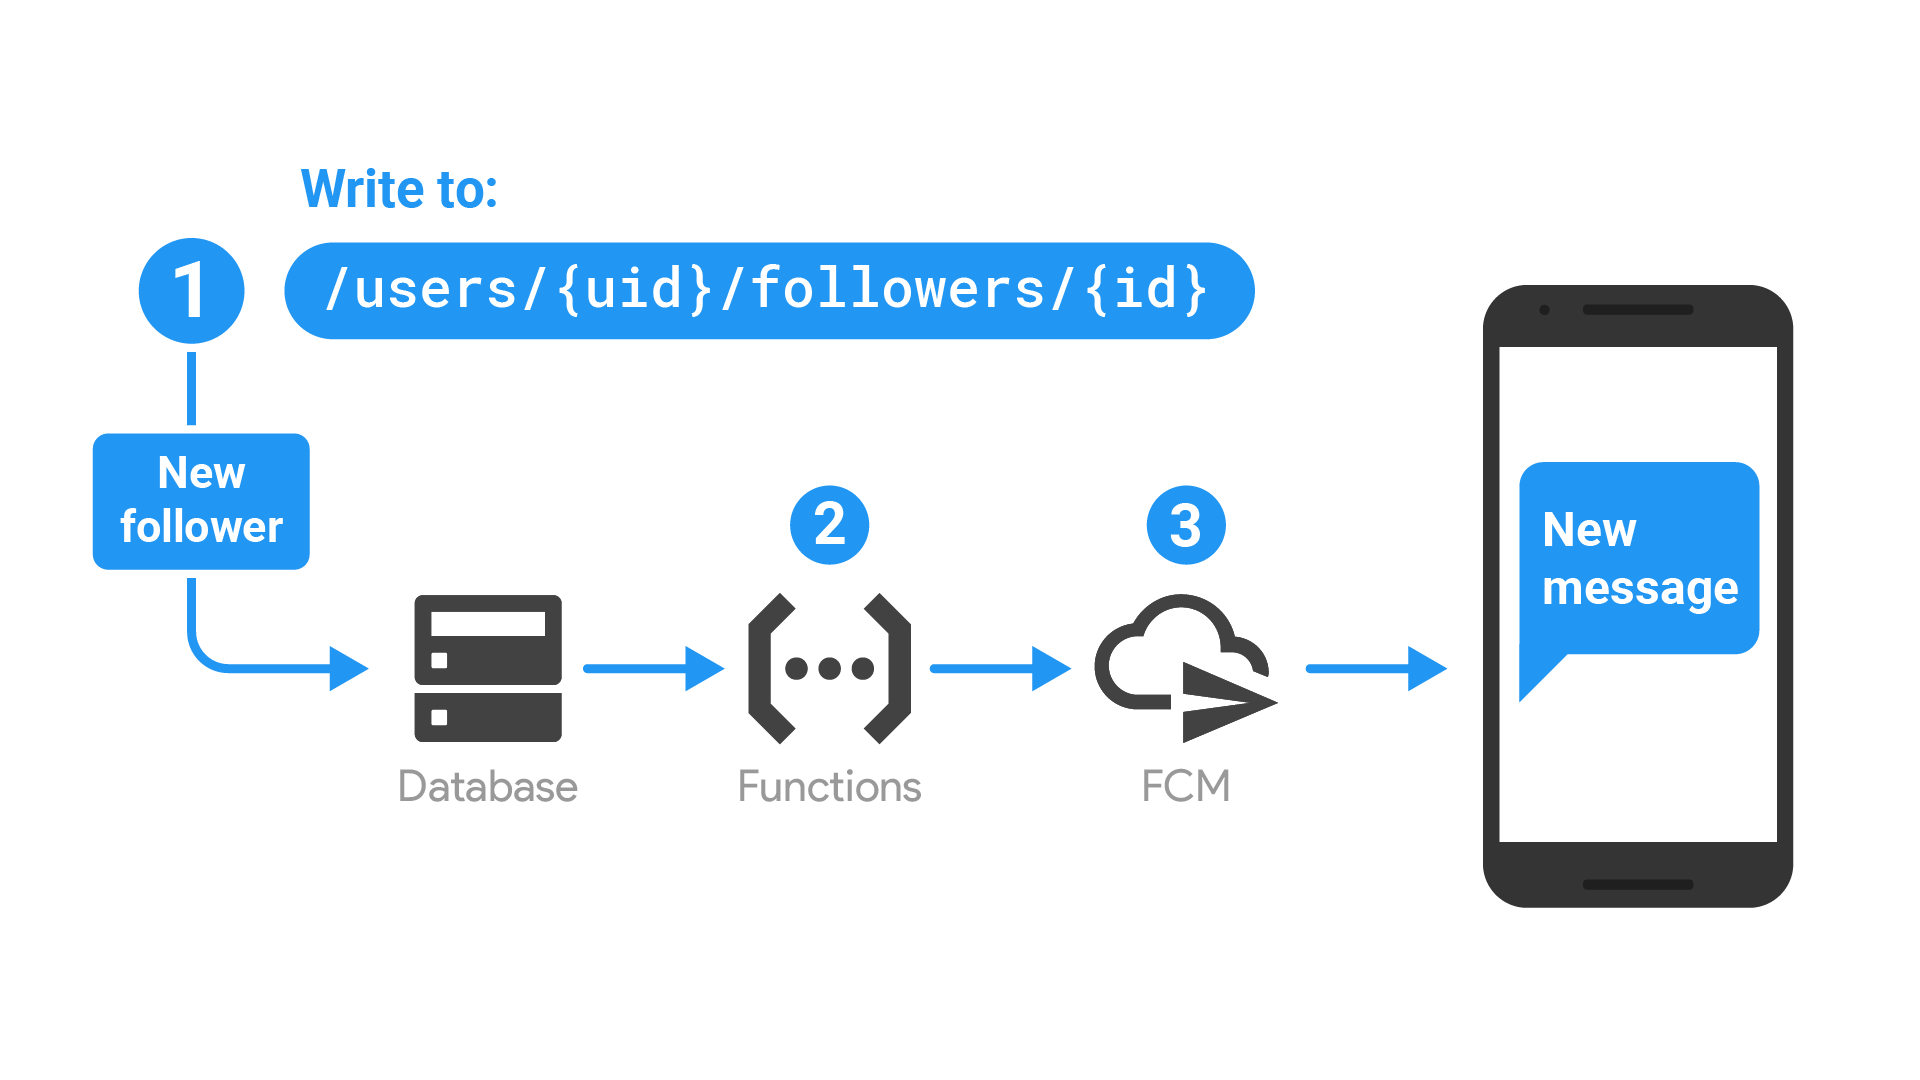
\includegraphics[scale=0.2]{Theoretische_Grundlagen/images/firebase_functions_notify.png}
	\end{center}
	\caption{Cloud Functions Anwendungsfall Benachrichtigung}
	\label{fig:functions_notifications}
\end{figure}
In Abbildung \ref{fig:functions_notifications} ist ein typischer Anwendungsfall beschrieben. 
Ein Event auf der Datenbank wird ausgelöst, hier ein neuer Nutzer folgt einem weiteren Nutzer.
Es wird also ein Dokument in der Unter-Sammlung \texttt{followers} erzeugt. Diese Unter-Sammlung befindet sich innerhalb des Dokumentes \texttt{uid} der Sammlung \texttt{users}.
Im zweiten Schritt erstellt die Funktion eine Nachricht, welche über Firebase Cloud Messaging (FCM) versendet werden soll.
Über abgespeicherte Tokens sendet FCM die Benachrichtigung an das Gerät des Nuters \texttt{uid}.\cite{firebase2021}
\subsubsection{Cloud Messaging}
Firebase Cloud Messaging ist eine plattformübergreifende Messaging-Lösung zum zuverlässigen Versenden von Nachrichten an Nutzergeräte.
In Abbildung \ref{fig:cloudmessaging_architecture} ist die Architektur dieses Tools dargestellt.
Hierbei wird es grundlegend in das Erstellen, Transportieren und Empfangen der Nachrichten unterteilt.\cite{firebase2021}\\
\begin{itemize}
	\item \textbf{Erstellen} Die zu versendenden Nachrichten können, wie in Kapitel \ref{sec:cloudfunctions} beschrieben, manuell oder automatisiert erzeugt werden. 
	Bei der Automatisierung ist wichtig, dass die Nachrichten in einer vertrauenswürdigen Serverumgebung erstellt werden, damit alle Nachrichtentypen unterstützt werden (Schritt 1). 
	Das FCM Backend akzeptiert dann in Schritt 2 Nachrichtenanfragen, ordnet die Nachrichten verschiedenen Themen zu und erzeugt unter anderem Metadaten für Nachrichten, wie bspw. die Nachricht ID. 
	\item \textbf{Transportieren} Die Nachrichten werden hierbei an die entsprechenden Geräte weitergeleitet.
	Da verschiedene Geräte auf unterschiedlichen Plattformen basieren, muss die Transportschicht auf Plattformebene arbeiten.
	Hierfür werden folgende Ebenen genutzt:
	\begin{itemize}
		\item Android Transport Layer (ATL) für Android-Geräte mit Google Play-Diensten
		\item Apple Push Notification Service (APNs) für iOS-Geräte
		\item Web-Push-Protokoll für Web-Apps
	\end{itemize}
	\item \textbf{Empfangen} Das FCM SDK behandelt die Benachrichtigung oder Nachricht. Dies ist abhängig vom Vorder-/ Hintergrundstatus der Anwendung und der jeweiligen Anwendungslogik.
\end{itemize}


\begin{figure}[htb]
	\begin{center}
		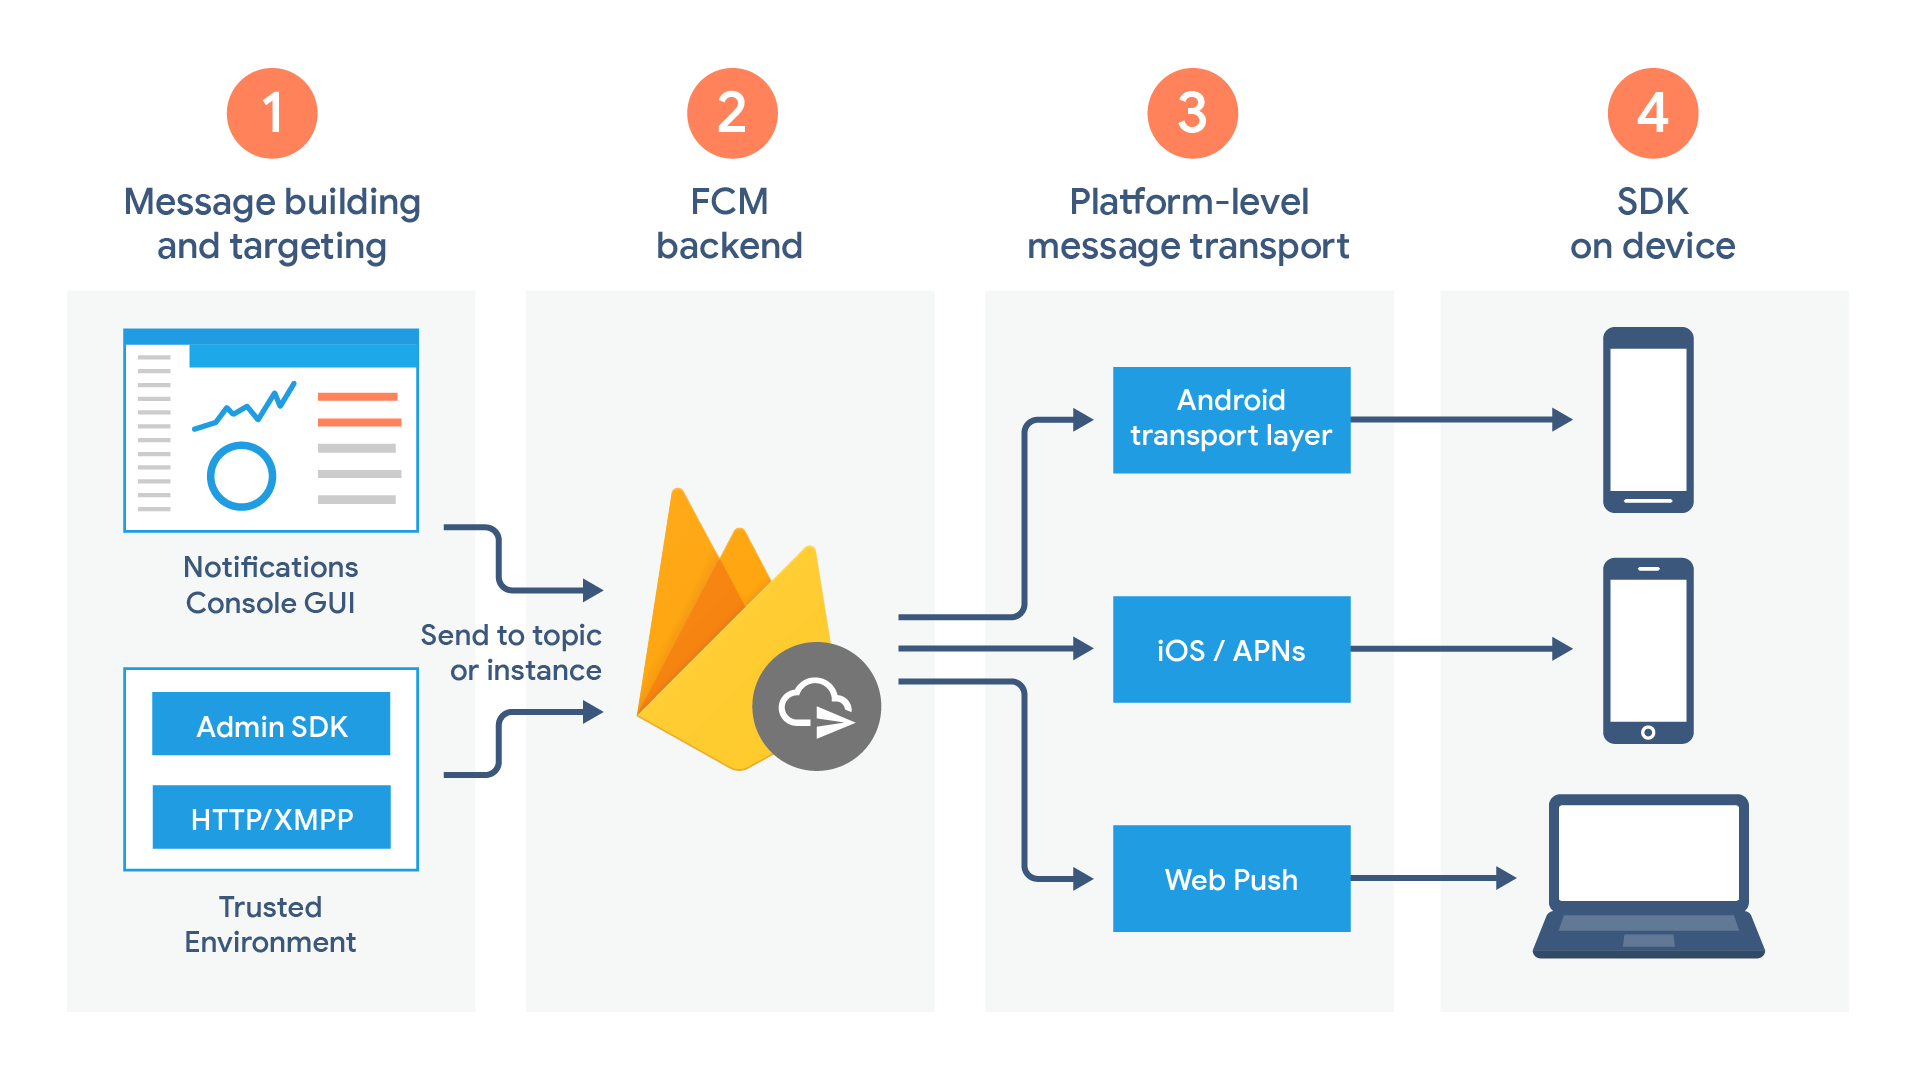
\includegraphics[scale=0.23]{Theoretische_Grundlagen/images/firebase_cloudmessaging_architecture.png}
	\end{center}
	\caption{Firebase Cloud Messaging Architektur}
	\label{fig:cloudmessaging_architecture}
\end{figure}

\subsubsection{Google AdMob}
Google AdMob bietet eine einfache Art, gezielte Werbung innerhalb der Anwendung zu schalten und somit die Anwendung zu monetarisieren.
Zusätzlich bietet das Tool in Kombination mit Google Analytics\footnote{Ein freies Analysetool, welches über alle Tools hinweg Ereignisse sammelt und diese Werte direkt graphisch darstellt. Da es für die Implementierung nicht weiter relevant ist, wird es nicht detaillierter besprochen. Zusätzliche Informationen unter \href{https://firebase.google.com/docs/analytics}{firebase.google.com}.} zusätzliche Anwendungsdaten und Analysefähigkeiten.\\
Werbung lässt sich in unterschiedlicher Weise anzeigen (siehe Abbildung \ref{fig:firebase_admob}) und lässt sich reibungslos in UI Komponenten integrieren. 
Verschiedene Features sind hier jedoch plattformabhängig. 
Auf der Android Plattform ist es für Nutzer möglich, beworbene Produkte direkt aus der Anwendung heraus zu kaufen.\\
Ein weiteres Werbetool \textit{Google Mobile Ads SDK} ist eine alleinstehende SDK, hingegen Google AdMob bietet einfache Integration in Firebase und weitere Tools.\cite{firebase2021}

\begin{figure}[tbt]
	\begin{center}
		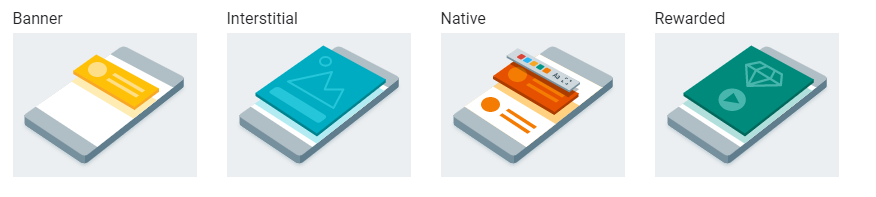
\includegraphics[scale=0.55]{Theoretische_Grundlagen/images/firebase_admob_ads.PNG}
	\end{center}
	\caption{Google AdMob Anzeigemöglichkeiten}
	\label{fig:firebase_admob}
\end{figure}





































\subsection{Anwendungsentwicklung für mobile Endgeräte}
\label{sec:mobile_development}
Mobile Geräte sind heutzutage ein sehr großer Teil unseres Tagesablaufs. Durchschnittlich verbringen wir 3:54 Stunden pro Tag an mobilen Geräten (hier bezogen aus Bürger der USA). Die meiste Zeit hiervon wird in Apps (ca. 90\%). \footnote{\url{https://www.emarketer.com/content/us-time-spent-with-mobile-2019}, letzter Zugriff: 26. Februar 2021}
Laut Cisco wird dieser Markt sich jedoch nicht nur auf Industrieländer beruhen, sondern bis 2023 sollen weltweit 71\% der Bevölkerung mobile Konnektivität haben \cite{cisco2020}.
Diese Entwicklung forcierte viele Firmen immer mehr ihre Anwendungen auch \textit{mobile ready} zu gestalten. Dies kann man bspw. deutlich bei der Anpassung vieler Webseiten an Mobile Seiten- und Größenverhältnisse oder auch dem Anbieten von \textit{Apps}, welche bereits für Desktop o.ä. verfügbar waren, erkennen. \\

\noindent
Daher ist es für die Wirtschaft und Entwicklung gleichermaßen wichtig sich ständig weiterzuentwickeln und sich nicht auf (kosten-) ineffizienten Entwicklungsprozessen auszuruhen. Dabei bieten jährliche, wenn nicht sogar halbjährliche Design- und Performanceänderungen von den Geräten selbst oder der Betriebssysteme Herausforderungen an die mobilen Anwendungen - \textit{apps} - und gleichzeitig an deren Programmierumgebung. Trotz einer riesigen Auswahl an \textit{Apps} lassen sich diese allgemein in drei Kategorien eingliedern: Plattformspezifische native Anwendungen, adaptive Webanwendungen und plattformübergreifende Anwendungen.

\subsubsection{Begriffe}
\noindent
\hangindent1cm
\textbf{Eine Plattform:} besteht aus der Hardware (System und zusätzlicher Peripherie, wie Sensoren oder Aktoren), dem Betriebssystem, den spezifischen \textit{Software Development Kits (SDK)} und den jeweiligen Basisbibliotheken. 
Zusammen bietet eine Plattform die Grundlage um Software für sie zu entwickeln.

\noindent
\hangindent1cm
\textbf{Ein Framework:} definiert eine Architektur für Anwendungen und stellt Komponenten bereit, mit welchen das Entwickeln einer Anwendung erleichtert sein soll \cite{johnson1988}.
Ein platt"-form"-über"-grei"-fendes Framework muss somit Anwendungscode für mehrere Plattformen wiederverwenden, jedoch müssen auch plattformspezifische Funktionen, wie Architektur oder Benutzeroberflächen API, bereitgestellt werden. Mehr dazu in Kapitel \ref{plattformuebergreifende_anwendungen}.

\noindent
\hangindent1cm
\textbf{Eine mobile Anwendung:} ist eine Anwendung, geschrieben für eine Plattform eines mobilen Endgerätes, welche die jeweiligen Features nutzen könnte - dazu zählen Kamera(s), Beschleunigungssensoren oder auch \textit{Global Positioning System (GPS)}. Webseiten als solches sind demnach keine mobilen Anwendungen.


\subsubsection{Plattformspezifische native Apps}
Plattformspezifische oder auch native Anwendungen sind Programme, welche auf eine gewisse Plattform abzielen und in einer der davon unterstützen Programmiersprachen geschrieben wurden. Da diese Art der (mobilen) Anwendung mit plattformspezifischen  SDK und \textit{Frameworks} entwickelt wird, ist diese Anwendung an eine Plattform gebunden. \\
Dies bringt zum einen natürlich Vorteile wie allgemein best mögliche Performance auf der jeweiligen Plattform und direkt vom Hersteller unterstützte Entwicklungsumgebungen/SDKs.
Zudem lassen sich plattformspezifische Fähigkeiten oder Einstellungen nutzen - beispielsweise mehrere Kameras oder GPS.

\noindent
Gleichzeitig beschränkt man sich aber logischerweise auf eine Plattform und deckt mit einer Anwendung nur einen Teil des gesamten Marktes. Dies bringt im Vergleich zu den anderen Möglichkeiten einen deutlich erhöhten Entwicklungs- und Wartungsaufwand mit sich, da für andere Plattformen Programmcode nicht übernommen werden kann. Zusätzlich benötigen Entwickler spezifische Kompetenzen für beide Plattform und Entwicklungsumgebungen. \\

\noindent
Zwei der am weitesten verbreiteten Plattformen sind Android von Google und iOS von Apple. Anwendungen für Android können in Kotlin oder Java als Programmiersprache beispielsweise in dem \textit{integrated development environment (IDE)} von Google Android Studio entwickelt werden. Für iOS wird hingegen mit Objective-C und Swift als Programmiersprache primär in der IDE XCode entwickelt.

\noindent
Beide bieten jeweils Plattform eigene Services an, beispielsweise das direkte Veröffentlichen in den jeweiligen Appstore \cite{fentaw2020}.

\subsubsection{Plattformübergreifende Anwendungen}
\label{plattformuebergreifende_anwendungen}
Die Entwicklung einer plattformübergreifenden Anwendung zeichnet sich generell durch die Möglichkeit aus, nur einmal Code schreiben zu müssen, diesen jedoch auf mehreren Plattformen ausführen zu können. \\
Verschiedene Ansätze einer solchen Anwendung sind in Abbildung \ref{fig:crossplattform_architecture} kategorisiert. Im Folgenden werden jene Entwicklungsmöglichkeiten detaillierter besprochen.

\begin{figure}[tbt]
	\begin{center}
		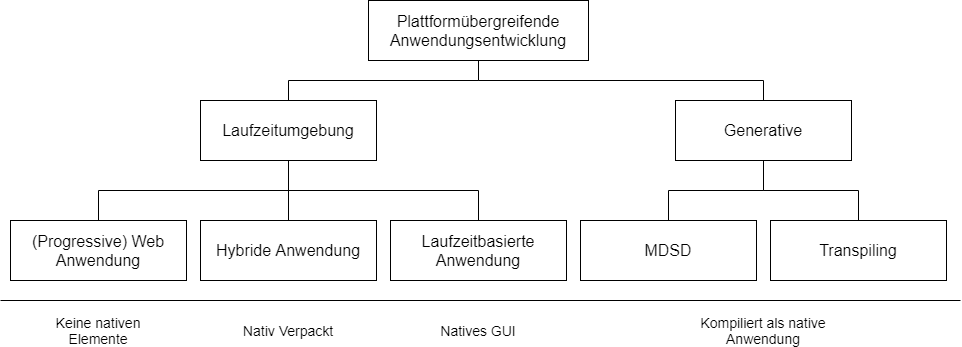
\includegraphics[scale=0.47]{Theoretische_Grundlagen/images/crossplattform_unterteilung.png}
	\end{center}
	\caption[Kategorisierung verschiedener plattformübergreifender Ansätze]{Kategorisierung verschiedener plattformübergreifender Ansätze. Erstellt nach \cite{majchrzak2015} \protect}
	\label{fig:crossplattform_architecture}
\end{figure}

\paragraph{\textit{(Progressive) Web Apps}}
Eine mobile Webanwendung ist eigentlich eine Webseite, welche sich an die Größe und Auflösung von unterschiedlichen Bildschirmen anpasst - hier speziell an die Bildschirmgrößen der mobilen Geräte. Diese Anwendung ist mit Standard Webentwicklungstools geschrieben (HTML, CSS \& JavaScript) und läuft somit theoretisch auf jedem Gerät mit einem Internet Browser \cite{charland2011}.
Aufgrund der steigenden Unterstützung von jeglichen APIs in mobilen Browsern, ist es auch möglich geworden auf Geräteeigenschaften, wie bspw. den Standort zuzugreifen.\\
Jedoch kann diese App logischerweise nicht im jeweiligen \textit{Appstore} heruntergeladen werden, da es sich weiterhin um eine Webseite handelt.
Aus gleichem Grund kann hiermit auch kein \glqq natives Design und Leistung\grqq erzeugt werden.\\

\noindent
Abhilfe hierfür sorgt jedoch die von Google vorgestellte Design Idee \textit{Progressive Web Apps} (PWA). Sie bietet die Möglichkeit Code in sogenannte \textit{service worker} als Hintergrundthread ausführen zu lassen, ein Webseiten Manifest anzugeben, die App offline bedienen zu können und bieten die Möglichkeit die PWA zu installieren. Gleichzeitig kann mit diesem Design eine zu nativen Apps vergleichbare Leistung erreicht werden \cite{bjorn-hansen2020}. \\

\noindent
Generell ist der Ansatz sehr simpel, da hiermit plattformübergreifende Anwendungen geschrieben werden können, welche sich auf allen Geräten mit Browser bedienen lassen.
Hierfür wird zudem keine zusätzliche Programmiersprache oder wissen über die jeweilige Plattform benötigt.\\
Eine große Schwierigkeit hieran ist weiterhin der Zugriff auf Gerätefeatures, da nicht alle über den Browser verfügbar sind.

\paragraph{Hybride Anwendungen}
\label{hybride_anwendung}
Eine hybride Anwendung kombiniert die native Vorgehensweise mit der einer normalen Webseite. 
In einer nativen WebView ist eine Webanwendung verpackt, welche nun in einer \textit{HTML-Rendering-Engine} gerendert wird. Bei Android und iOS ist das WebKit.
Diese WebView funktioniert ähnlich wie ein normaler Browser, jedoch werden Kontrollfenster nicht angezeigt, wie zum Beispiel Adresszeile, Einstellungen oder Lesezeichen.
Ähnlich wie bei Web Anwendungen werden über JavaScript APIs Gerätefeatures eingebunden.\\
Ein sehr frühes Framework für diese Art von Anwendung war \href{https://cordova.apache.org/}{Adobe Cordova}, eher bekannt als das ursprüngliche PhoneGap von Nitobi. Viele weitere Frameworks basieren auf ihren Anfängen.\\

\noindent
Eine hybride Anwendung kann also normal als App im \textit{Appstore} heruntergeladen auf dem Gerät installiert und offline genutzt werden - also sehr ähnlich zu nativen Lösungen. Daher ist dieser Ansatz auch sehr beliebt
Daher liegt auch hier die Leitung der Applikation deutlich hinter der der Nativen \cite{lachgar2017} \cite{bjorn-hansen2020}.

\begin{figure}[tbt]
	\begin{center}
		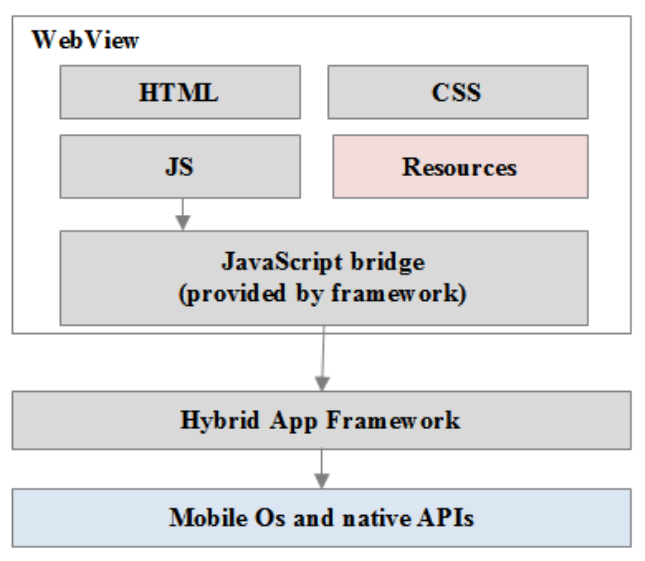
\includegraphics[scale=0.45]{images/hybride-anwendungen-struktur.PNG}
	\end{center}
	\caption[Struktur einer hybriden Anwendung]{Struktur einer hybriden Anwendung \protect \footnotemark}
	\label{fig:hybrid_structure}
\end{figure}
\footnotetext{Quelle: \cite{lachgar2017}}

\paragraph{Runtime basierte Anwendungen}
\label{runtime_based_apps}
Im Gegensatz zur in Kapitel \ref{hybride_anwendung} beschriebenen hybriden Anwendung, nutzen Runtime basierte Anwendungen keinen Browser des Gerätes mit einer WebView, sondern jede App besitzt eine eigene Runtime Ebene. 
Jedes Framework muss also eine solche Ebene für alle Plattformen in jeweiliger Programmiersprache mitliefern, damit seine Anwendung hierauf laufen können.
Die Anwendungen hingegen sind dann beispielsweise in JavaScript (bspw. \href{https://reactnative.dev/}{React Native} oder \href{https://nativescript.org/}{NativeScript}), C\# (\href{https://dotnet.microsoft.com/apps/xamarin}{Xamarin}) oder sonstigen Programmiersprachen (bspw. \href{https://www.qt.io/}{Qt}) geschrieben.\\
\\
Jedem Framework-Entwickler ist die Freiheit gegeben, wie man die Anbindung an native Funktionen regelt. Bei hybriden Anwendungen ist dies durch die WebView Cordova festgelegt.
Typisch für Anwendungen dieser Art jedoch ist ein Plug-In-basiertes \textit{bridging System}. Es ermöglicht den Aufruf von fremden Funktionsinterfaces in plattformspezifischem Code.
Somit können beispielsweise React Native und NativeScript mit Sprachinterpretern (bspw. JavaScriptCore und V8) auf den Geräten Auszeichnungssprache (hier HTML (Hypertext Markup Language)) interpretieren und plattformspezifische Komponenten der Benutzeroberflächen erzeugen.\\
\\
Ein großer Nachteil dieser Strategie ist jedoch zugleich ihr Vorteil: Jedes Framework besitzt seine eigene Architektur. Dadurch sind Plug-ins des einen Frameworks trotz gleicher Anwendungssprache nicht unbedingt funktionstüchtig im anderen. 
Bei projektspezifischen Plug-ins macht es einen späteren Systemwechsel daher besonders schwer, da nicht nur Benutzeroberfläche und Businesslogik neu geschrieben werden müssen, sondern auch jeweilige Plug-ins \cite{bjorn-hansen2020}.

\paragraph{Model-driven Software Entwicklung}
Die Grundsätze der modellgetriebenen Softwareentwicklung beschäftigen sich mit der Abstraktion des Modells als (Teil eines) System, von welchem die eigentliche Software abgeleitet wird \cite{stahl2006}.\\
Das bedeutet in der Realität, dass eine höhere Abstraktion als Quellcode in Form von textuellen oder grafischen domänenspezifischen Sprachen oder universell einsetzbaren Modellierungssprachen (Unified Modeling Language(UML)) zum beschreiben der Software verwendet wird. 
Codegeneratoren übersetzen diese Modelle nun jeweils in Programmiersprachen der gewählten Zielplattform, auf welcher sie kompiliert werden.\\
\\
Theoretisch kann hierdurch der komplette Funktionsumfang wie bei einer nativen Anwendung erreicht werden.
Bekannte Frameworks dieser Methode sind zum Beispiel \href{https://www.wi.uni-muenster.de/sites/wi/files/public/department/pi/publications/heitkoetter/cross-platform-model-driven-development-of-mobile-applications-with-md2.pdf}{$M\!D_2$}, \href{https://www.sciencedirect.com/science/article/abs/pii/S1477842417301215}{MAML}, \href{https://www.webratio.com/site/content/en/home}{WebRatio Mobile}, \href{https://www.biznessapps.com/}{BiznessApps} und \href{https://bubble.io/}{Bubble}.\\
\\
Der große Nachteil hieran ist, dass Entwickler sehr selten modellgetriebene Entwicklung verwenden, sondern Quellcode-basierte Programmiermethoden bevorzugen \cite{bjorn-hansen2020}.
\paragraph{Kompilierte Anwendungen}
\label{compilierte_anwendungen}
Kompilierte plattformübergreifende Anwendungen basieren auf einer einzigen Codebasis und können für mehrere Plattformen vollständig kompiliert werden. 
Dies kann entweder von der Codebasis einer nativen Anwendung für mindestens eine andere Plattform (bspw. \href{https://developers.google.com/j2objc/}{J2ObjC}), oder von einer unabhängigen Codebasis direkt für mehrere Plattformen (bspw. \href{https://flutter.dev/}{Flutter}) geschehen.
Hierbei ist Flutter für diesen Anwendungsfall am interessantesten und wird in Kapitel \ref{flutter} näher behandelt.\\
Ein Hindernis dieser Art ist die erhöhte Komplexität der einzelnen Frameworks.

\subsection{Frameworks zur mobilen, plattformübergreifenden Entwicklung}
\label{sec:framework}
In den folgenden Kapiteln werden einzelne Frameworks zur mobilen, plattformübergreifenden Entwicklung vorgestellt.\\
In der Statistik \ref{fig:crossplattform_popularity} aus dem Jahr 2020 ist React-Native das beliebteste Framework, dicht gefolgt von Flutter. 
Wie man deutlich hier auch sehen kann, haben andere, bisher auch sehr erfolgreiche Frameworks einen enormen Rückgang von teilweise über einem Drittel ihrer Nutzer erleben müssen. \\
\\
Aus diesen Gründen werden im weiteren Verlauf nur die Frameworks React-Native und Flutter weiter besprochen.

\begin{figure}[tbt]
	\begin{center}
		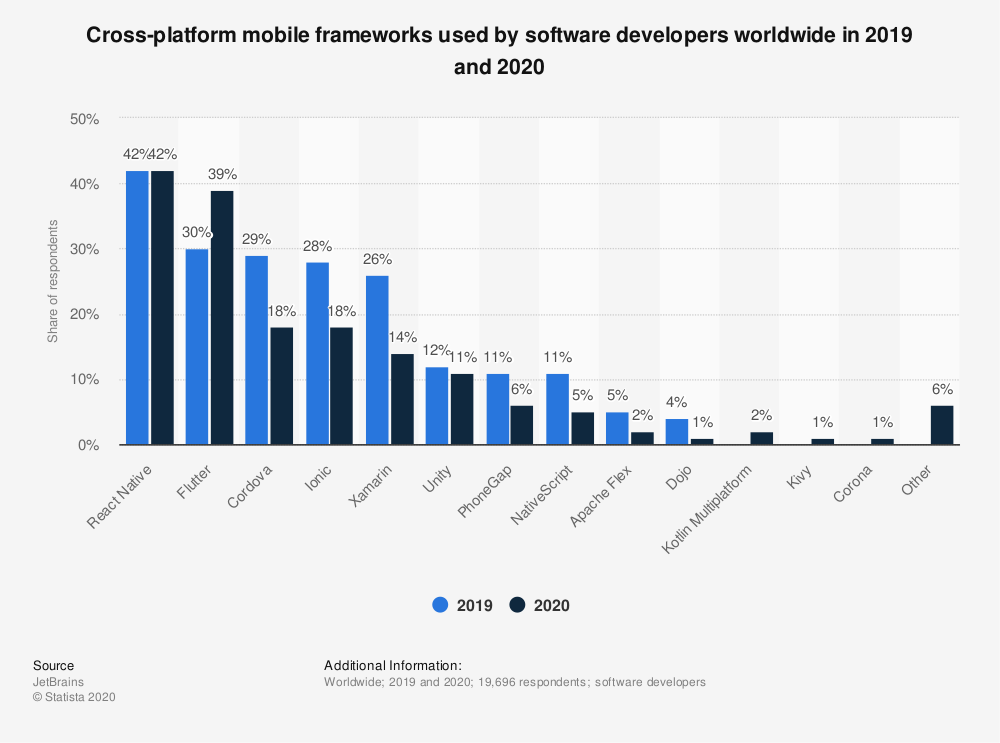
\includegraphics[scale=0.4]{Theoretische_Grundlagen/images/crossplattform_popularity.png}
	\end{center}
	\caption[Beliebtheit nach Framework im Bereich der plattformübergreifenden mobilen Entwicklung]{Beliebtheit nach Framework im Bereich der plattformübergreifenden mobilen Entwicklung \protect \footnotemark}
	\label{fig:crossplattform_popularity}
\end{figure}
\footnotetext{Quelle: \url{https://www.statista.com/statistics/869224/worldwide-software-developer-working-hours/}, letztern Zugriff: 22. April 2021}

\subsubsection{React Native}
\label{react-native}
React Native ist ein open source Framework, welches von Facebook 2015 veröffentlicht wurde. 
Es basiert auf dem bekannten Web-Framework \href{https://reactjs.org/}{\textit{React}} (ebenfalls von Facebook) und bringt daher den deklarativen und Komponenten-basierten Stil mit sich. 
Die Programmiersprache ist aus diesem Hintergrund auch logischerweise JavaScript.
Das Framework an sich ist in verschiedenen Sprachen implementiert: JavaScript, Swift, Objective-C, C++ und Python.\\
\\
Allgemein bietet das Framework die Möglichkeit plattformübergreifende Apps für iOS, Android und für Windows zu schreiben. Hierbei wird der geschriebene Code in einer JavaScript Laufzeitumgebung ausgeführt (React Native selbst verwendet generell \href{https://trac.webkit.org/wiki/JavaScriptCore}{JSC (JavaScriptCore)}, seit neuestem kommt auch \href{https://hermesengine.dev/}{Hermes} zum Einsatz, jedoch sind auch andere bekannte Umgebungen denkbar - bspw. \href{https://v8.dev/}{V8} in Chrome) es lässt sich zu den Runtime-basierten Anwendungen in Kapitel \ref{runtime_based_apps} zuordnen \cite{reactnative2021}.\\
\paragraph{Architektur}
Grundlegend wurde React Native als Plattform-agnostisch designt. Entwickler schreiben also plattformunabhängigen JavaScript React Code, während das Framework den erstellten React Baum in Plattform-spezifischen Code umschreibt. Hierbei wurde 2013 (noch intern) die Web-Technologie React mit nativen Plattformen (nur interne) vereint, jedoch war dieses Design aufgrund eines einzigen Threads sehr langsam. Um dies zu verbessern basierte das Framework lange Zeit auf drei unterschiedlichen Threads, welche über eine Brücke verbunden sind.

\begin{figure}[tbt]
	\begin{subfigure}{\textwidth}
		\centering
		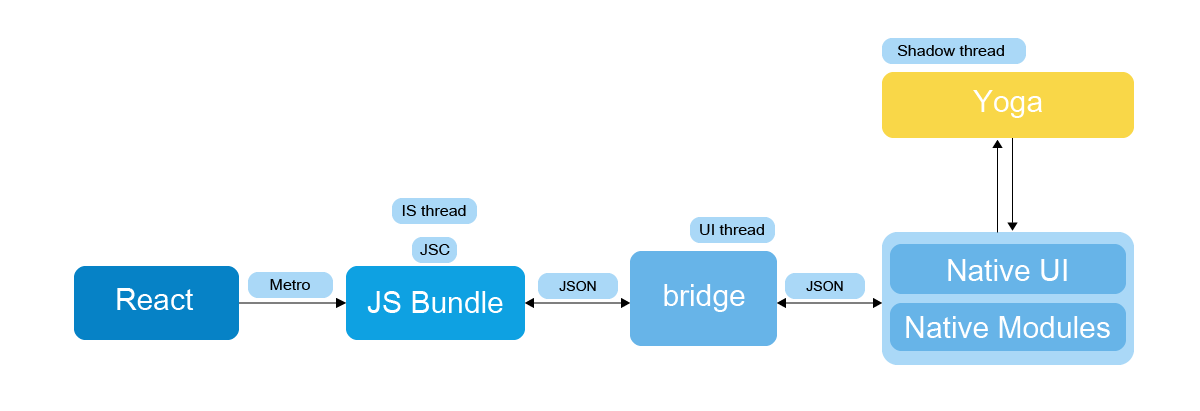
\includegraphics[scale=0.4]{Theoretische_Grundlagen/images/reactnative_architecture_old.png}
		\caption{}
		\label{fig:reactnative_architecture_old}
	\end{subfigure}\\
	\begin{subfigure}{\textwidth}
		\centering
		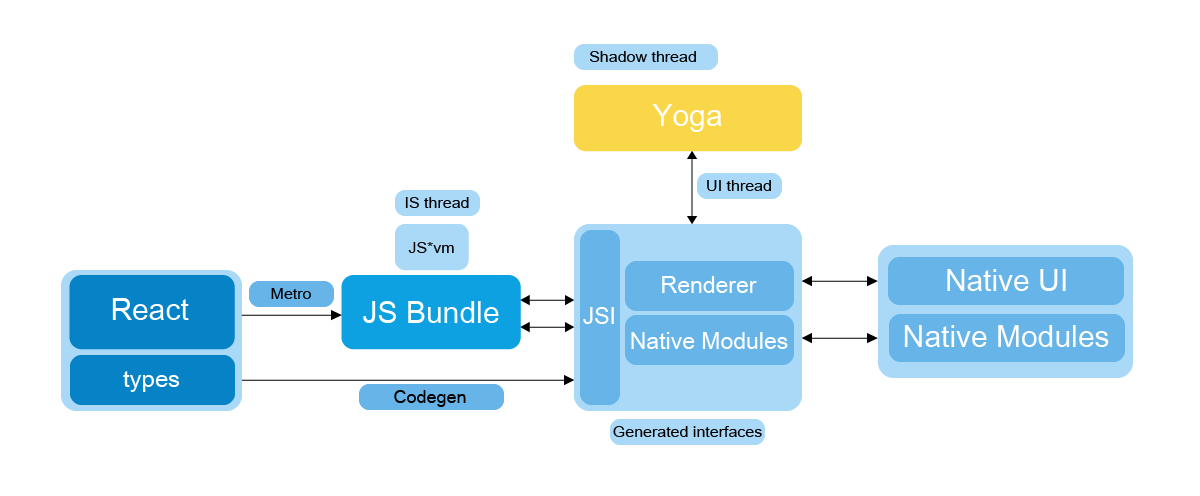
\includegraphics[scale=0.4]{Theoretische_Grundlagen/images/reactnative_architecture.png}
		\caption{}
		\label{fig:reactnative_architecture}
	\end{subfigure}
	\caption[Alte und neue Architektur von React Native]{(a) Alte und (b) neue Architektur von React Native \protect \footnotemark}
\end{figure}
\footnotetext{Quelle: \url{https://litslink.com/blog/new-react-native-architecture}, letzter Zugriff: 15. April 2021}

\begin{itemize}
	\item \textit{JavaScript Thread}. Hier wird der gesamte JavaScript Code abgelegt und interpretiert. Alles wird über die JSC Engine ausgeführt.
	\item \textit{Native Thread}. Die Benutzeroberfläche und Kommunikation mit dem JavaScript Thread steht hier im Mittelpunkt. Der gesamte native Code wird hier ausgeführt. Die Benutzeroberfläche wird dann aktualisiert, sobald die eben ein Änderung vom JS Thread vermittelt wird.
	\item \textit{Shadow Thread}. Hier wird das gesamte Layout der Anwendung berechnet. Zugrunde liegt die Facebook-eigene layout engine \glqq Yoga\grqq .
\end{itemize}

\noindent
Ein Hauptproblem dieses Ansatzes ist, dass die Brücke grundlegend eine asynchrone Warteschlange ist, da der JS Thread und der native Thread unabhängig voneinander arbeiten. Zusätzlich werden während der gesamten Datenübertragung die Daten im JSON Format serialisiert und deserialisiert .
Daher kann es zu Performance-Einbrüchen und somit zu schlechter Nutzererfahrung, durch bspw. Eingabeverzögerung, kommen.

\noindent
Nach der Ankündigung 2018 veröffentlichte Facebook im Juli 2020 die neue Architektur. Mit ihr wurde der Bottleneck (die Brücke) ersetzt durch das JavaScript Interface.
Es ermöglicht nicht nur die komplette Synchronisierung der beiden Threads, sondern auch die direkte Kommunikation untereinander - vor allem das Konzept von \glqq shared ownership\grqq ist hier tragend, weshalb auch keine Serialisierung mehr nötig ist.
Zudem  ist man nun nicht mehr an JSC gebunden, sondern kann auch jegliche hoch-performante JavaScript Engines als Laufzeitumgebung verwenden.
Native Module werden nun nur noch bei Bedarf geladen anstatt alle beim Start der App.\\
Weiter wurde veralteter Legacy-Code aus dem Kern von React Native entfernt und nicht-essenzielle Teile aus dem Kern ausgelagert. Die aktuelle Architektur von React Native ist  in Abbildung \ref{fig:reactnative_architecture} zu sehen.\footnote{Quelle: React Native's re-architecture (2020): \url{https://medium.com/swlh/react-natives-re-architecture-in-2020-9bb82659792c}, letzter Zugriff: 17. April 2021}

\paragraph{JSX mit nativen Komponenten}
React (Native) verwendet als Programmiersprache JSX. Diese ist eine syntaktische Erweiterung von JavaScript (\textbf{J}ava\textbf{S}cript e\textbf{X}tention), welche zur fundamentalen Beschreibung der Nutzeroberfläche dient. JSX wird in normale JavaScript Objekte kompiliert, weshalb es nicht zwingend ist. \\
\begin{lstlisting}[caption=JSX Hello World Element]
	const element = <h1>Hello, world!</h1>;
\end{lstlisting}
Mithilfe dieser losen Kopplung von UI-Code und dazugehöriger Logik schlägt React eine optionale Lösung zur \textit{Separation of Concerns} vor. Anstelle dessen ist es auch möglich die Technologien in Markup- und Logik-Dateien aufzuteilen. \\
Außerdem kann argumentiert werden, dass JSX nur eine weitere Template-Sprache sei, ähnlich HTML oder XAML. DIes ist nicht korrekt, da wie oben bereits erwähnt JSX lediglich eine syntaktische Erweiterung von Java"-Script ist, also inmitten von JSX Objekten JavaScript geschrieben werden kann.\\
Weiterhin ist interessant, dass JSX \href{https://owasp.org/www-community/attacks/xss/}{Cross Site Scripting} vorbeugt, indem der React DOM alle eingesetzten Werte zunächst in einen einfachen String konvertiert \cite{react2021}.
\begin{lstlisting}[caption=Native Komponenten, label=lst:jsx_native_component]
	import React from 'react';
	import { Text } from 'react-native';
	
	const Cat = () => {
		return (
		// <Text> as native component
		<Text>Hello, I am your cat!</Text>
		);
	}
	
	export default Cat;
\end{lstlisting}
In dem Codebeispiel \ref{lst:jsx_native_component} wird ein Element \texttt{Cat} erzeugt, welches als Beschreibung dessen dient, was letztendlich auf dem Bildschirm angezeigt wird. 
In diesem einfachen Beispiel wird die native Komponente \texttt{<Text>...</Text>} verwendet. 
Native Komponenten sind in nativem Code (Kotlin oder Java für Android, bzw. Swift oder Objective-C für iOS) implementierte Komponenten und können in Java"-Script Code aufgerufen werden.
Diese werden dann während der Laufzeit für die jeweilige Plattform erstellt.\\
\\
React Native bringt die wichtigsten Komponenten mit sich, die \textbf{Core Components}. Zusätzlich erlaubt das Framework jedoch auch eigene Komponenten nativ zu implementieren, welche dem jeweiligen Anwendungsfall angepasst werden können.\\

\paragraph{Komponenten}
Gleichzeitig erlaubt React Native aber auch wiederverwendbare Komponenten in JavaScript aus den Kernkomponenten zusammenzustellen.
Hierzu lassen sich einzelne Komponente ineinander verschachteln, um hier im Beispiel \ref{lst:reactnative_own_components} einen \texttt{Text} innerhalb einer \texttt{View}\footnote{Eine \texttt{View} ist die Basiskomponente einer Benutzeroberfläche. In einer \texttt{View} wiederum können weitere Views verschachtelt sein.} anzeigen zu lassen.
Zusätzlich ist es möglich sogenannte \glqq props\grqq \, also Eigenschaften (engl.: properties), ähnlich einer normalen Funktion mitzugeben.
In dem betrachteten Beispiel entspricht das den Namen einzelner Katzen, welche als Text angezeigt werden \cite{reactnative2021}.\\

\begin{lstlisting}[caption=Eigene Komponenten, label=lst:reactnative_own_components]
import React from 'react';
import { Text, View } from 'react-native';

// configurable props
const Cat = (props) => {
	return (
	<View>
	<Text>Hello, I am {props.name}!</Text>
	</View>
	);
}

const Cafe = () => {
	return (
	<View>
	// reusable
	<Cat name="Maru" />
	<Cat name="Jellylorum" />
	<Cat name="Spot" />
	</View>
	);
}

export default Cafe;
\end{lstlisting}


\paragraph{State}
Für eine interaktive Benutzeroberfläche fehlt jedoch noch das Kernprinzip eines deklarativen UI. Ein sogenannter \textit{State} wird verwendet um die Daten, welche sich mit der Zeit oder über Nutzerinteraktion ändern, auf der Oberfläche anzuzeigen. Dieses Konzept wird ebenfalls von dem zweiten Framework verwendet und ist in Abbildung \ref{fig:flutter_state} visualisiert.\\
\\
Seit v14.8 ermöglicht React (und auch React Native)  durch Hooks einer Funktion einen \textit{State} hinzuzufügen. Hooks sind Funktionen, welche es Entwicklern ermöglichen sich in React Features einzuhaken. Bisher wurde dies über Klassenkomponenten ermöglicht, wodurch es jedoch komplizierter ist \textit{stateful logic} zwischen Komponenten wiederzuverwenden. Daher entkoppelt man diese Logik von den Komponenten und erlaubt unter anderem das separate Testen.\\

\begin{lstlisting}[caption=State mit \texttt{useState} Hook, label=lst:reactnative_state]
	import React, { useState } from "react";
	import { Button, Text, View } from "react-native";
	
	const Cat = (props) => {
		// make isHungry stateful
		const [isHungry, setIsHungry] = useState(true);
		
		return (
		<View>
		<Text>
		// show text dependent on isHungry state
		I am {props.name}, and I am {isHungry ? "hungry" : "full"}!
		</Text>
		<Button
		onPress={() => {
				setIsHungry(false);
		}}
		disabled={!isHungry}
		title={isHungry ? "Pour me some milk, please!" : "Thank you!"}
		/>
		</View>
		);
	}
	
	const Cafe = () => {
		return (
		<>
		<Cat name="Munkustrap" />
		<Cat name="Spot" />
		</>
		);
	}
	
	export default Cafe;
\end{lstlisting}

\noindent
Im Beispiel \ref{lst:reactnative_state} wird in Zeile 6 der \texttt{useState}-Hook verwendet. Diese Funktion erzeugt eine State-Variable mit dem Initialwert \texttt{true} und erstellt gleichzeitig eine Funktion zur Änderung des States (\texttt{setIsHungry}). Daraufhin wird, abhängig ob die Katze hungrig ist, dies im Text angezeigt, der Knopf zum füttern (de-)aktiviert bzw. auch hier den Text verändert \cite{reactnative2021}.\\

\subsubsection{Flutter}
\label{flutter}
Flutter ist eine open-source SDK entwickelt von Google und ist geschrieben in C, C++ und Dart.
Auf Basis eines Codes erlaubt Flutter es gleichzeitig Anwendungen für Android, iOS, Web und Desktop zu erstellen und ist zudem die primäre Methode für Google Fuchsia, Googles Betriebssystem\footnote{Quelle: \url{https://fuchsia.dev/}}.
Als 2D Grafikbibliothek verwendet Flutter  \href{https://skia.org/}{Skia}, welche auch von Chrome, Firefox und Android verwendet wird. Zudem basiert Flutter auf der Dart-Plattform welche das Kompilieren auf 32-bit und 64-bit ARM Prozessoren, auf Intel x64 Prozessoren und in JavaScript ermöglicht (siehe Abbildung \ref{fig:dart_plattform}). Daher ist Flutter eine wie in Kap. \ref{compilierte_anwendungen} beschriebene kompilierte, plattformübergreifende Anwendung

\noindent
Während der Entwicklung werden Flutter-Apps in einer virtuellen Maschine (VM) gestartet, welche \textit{stateful hot reload} ermöglicht. Bei Änderungen muss die App so nicht komplett neu kompiliert werden, sondern sie erneuert sich während der Laufzeit. Bei der Veröffentlichung der App, wird sie in den Maschinencode der beschriebenen Plattformen übersetzt.\\

\begin{figure}[tbt]
	\begin{center}
		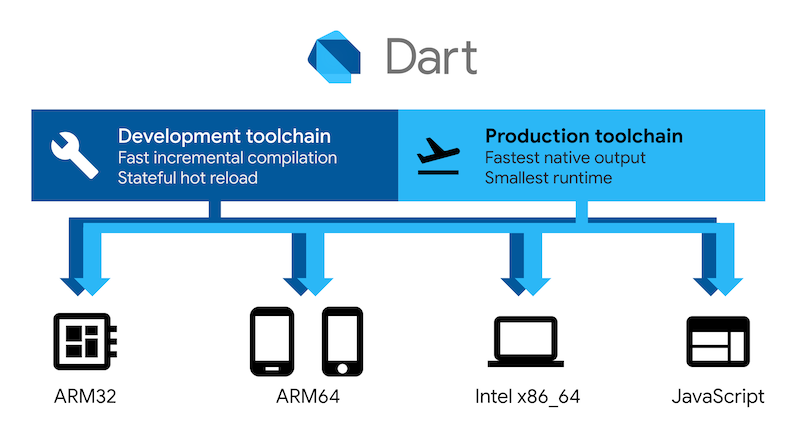
\includegraphics[scale=0.45]{Theoretische_Grundlagen/images/dart-diagram.png}
	\end{center}
	\caption[Kompatibilität der Dart Plattform]{Kompatibilität der Dart Plattform \protect \footnotemark}
	\label{fig:dart_plattform}
\end{figure}
\footnotetext{Quelle: \url{https://github.com/flutter/flutter}, letzter Zugriff; 12. April 2021}

\paragraph{Architektur}
\begin{displayquote}
	Flutter is designed as an extensible, layered system. It exists as a series of independent libraries that each depend on the underlying layer. No layer has privileged access to the layer below, and every part of the framework level is designed to be optional and replaceable\footnote{\url{https://flutter.dev/docs/resources/architectural-overview}}.
\end{displayquote}

\noindent
Grundlegend ist das Framework in drei Prozesseinheiten gegliedert. Diese bestehen wiederum jeweils aus, für sie charakteristischen APIs und Bibliotheken:\\

\noindent
\hangindent1cm
\textbf{Flutter embedder}: Der Einstiegspunkt in die jeweilige Plattform. Er koordiniert Zugriffe auf Services des Betriebssystems; er ist also zuständig für bspw. die Kommunikation mit dem Input Method Editor (IME) und den Lifecycle Events der App. Daher ist der Embedder in der, von der Plattform unterstützten Programmiersprache geschrieben: derzeit wird Java und C++ für Android, Objective-C/Objective-C++ für iOS und macOS, und C++ für Windows und Linux verwendet.\\

\noindent
\hangindent1cm
\textbf{Flutter Engine}: Der Kern von Flutter, geschrieben hauptsächlich in C und C++, ist die \textit{low-level} Implementierung der Flutter Kern Programmierschnittstelle (API). Daher ist sie zuständig für das graphische Darstellen (Rasterisierung) des Codes sobald ein neuer \textit{Frame} angezeigt werden muss. Im Flutter Framework wird die \textit{Engine} als dart:ui Bibliothek offengelegt - der zugrundeliegende C++ Code wird in Dart Klassen eingefügt.\\

\noindent
\hangindent1cm
\textbf{Flutter Framework}: Das Framework, mit welchem der Entwickler schlussendlich meistens arbeiten wird. Es ist in Dart geschrieben und bietet sogenannte \textit{Layer} für Animationen, Layout und Widgets. Widgets werden von Flutter als Einheit der Komposition von Benutzeroberflächen verwendet und sind als einzelne Bausteine zu verstehen, welche zusammengefügt ein Objekt oder sogar einen kompletten Bildschirm ergeben.\\

\noindent
Bei der Entwicklung mit Flutter wird ein Baum von Widgets erzeugt, welcher als Bauplan der Applikation angesehen werden kann. Nach diesem Plan wird mithilfe von States der einzelnen Widgets schlussendlich das User Interface (UI) gerendert \cite{flutter2021}.

\begin{figure}[tbt]
	\begin{center}
		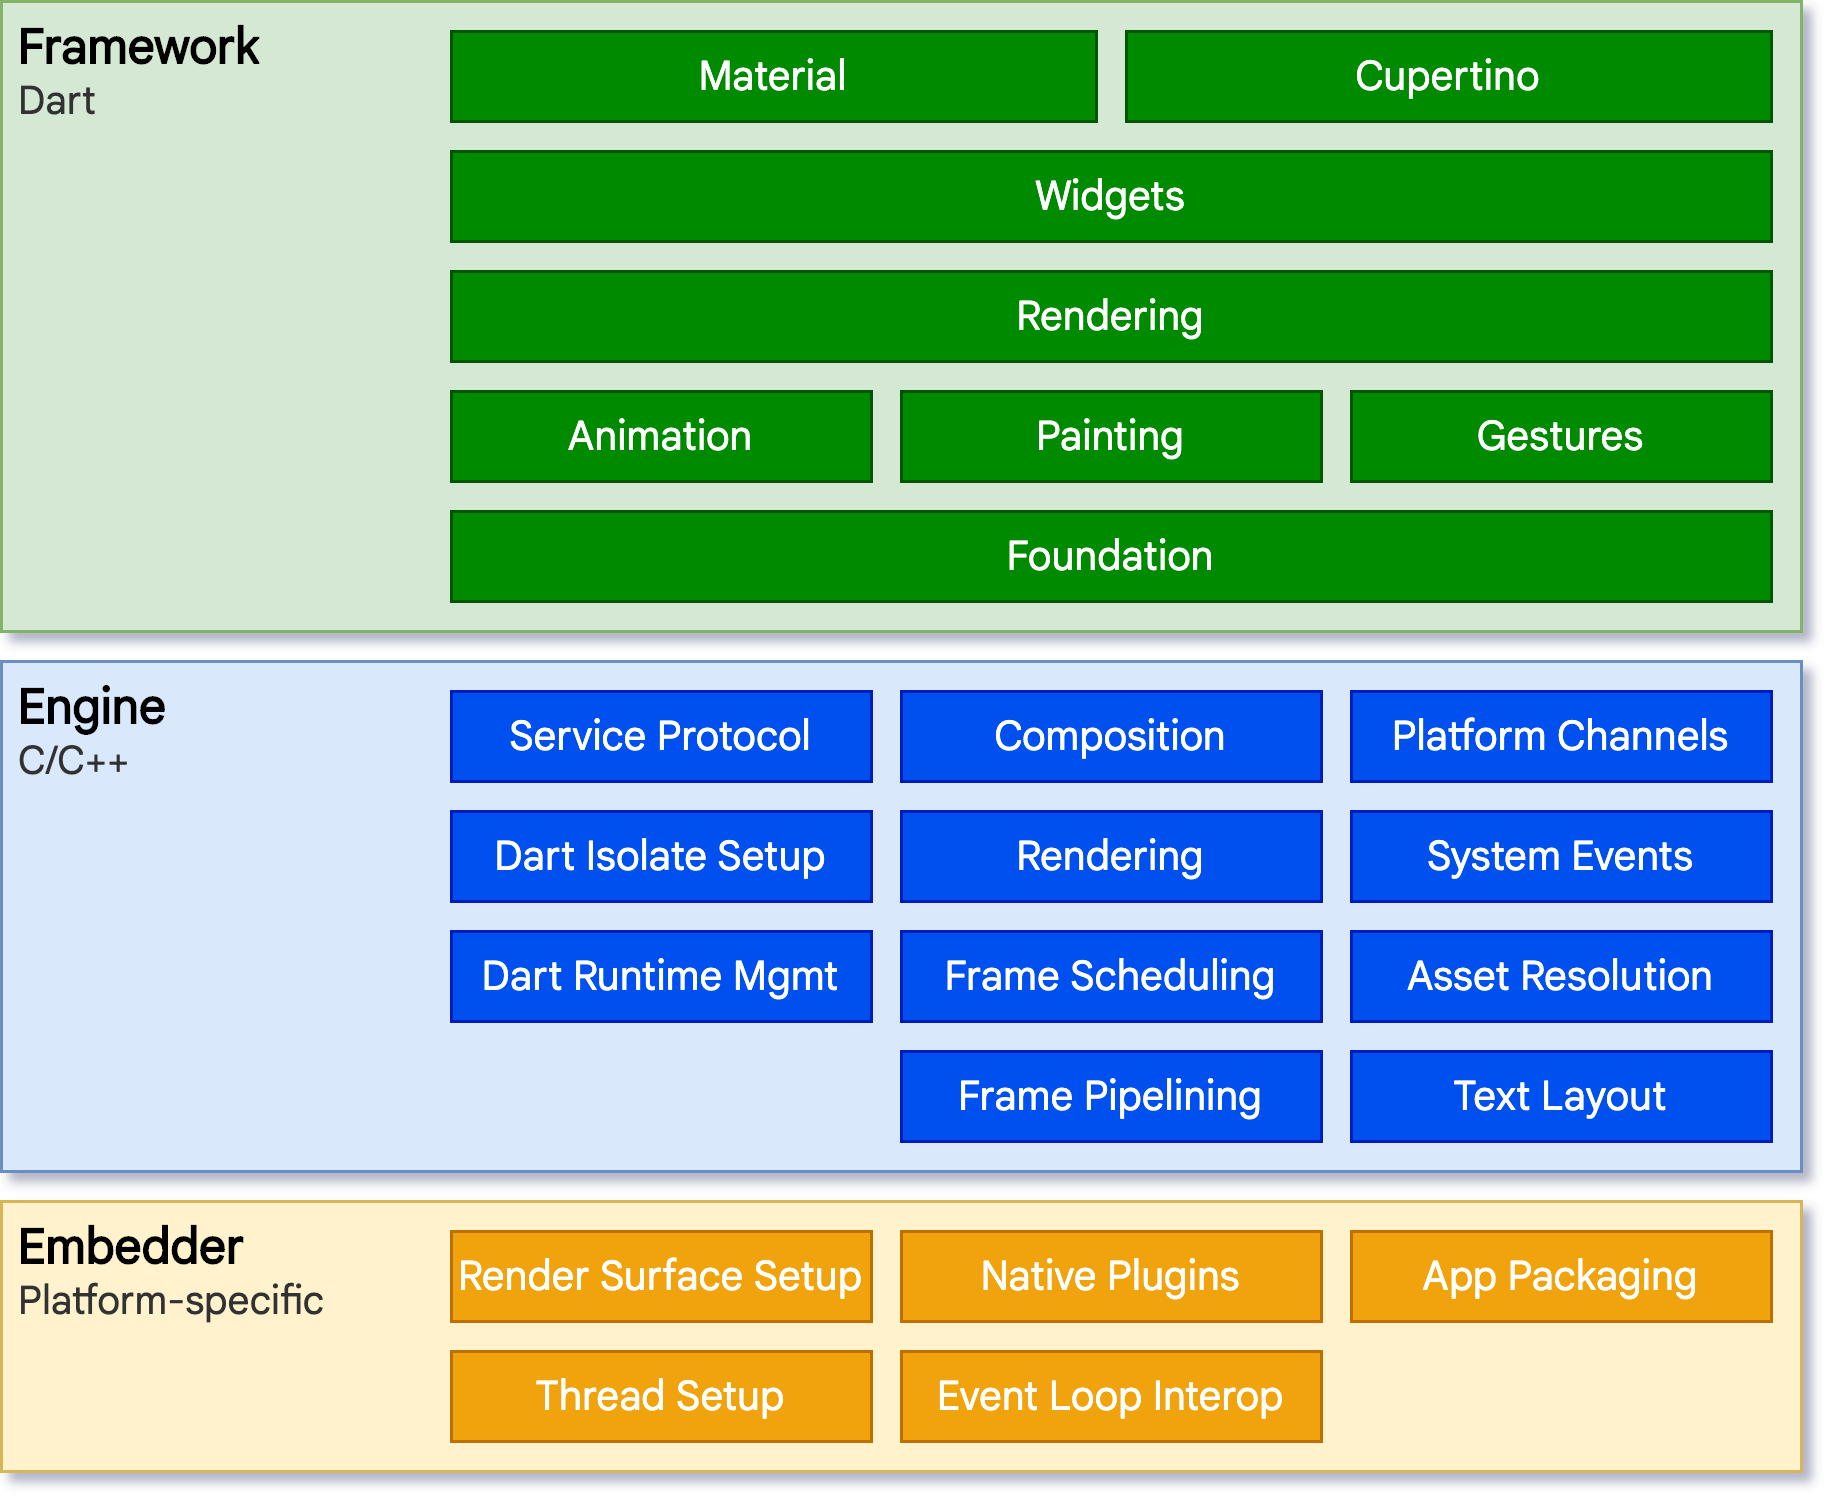
\includegraphics[scale=0.25]{Theoretische_Grundlagen/images/flutter_architektur.png}
	\end{center}
	\caption[Bibliotheken und Ebenen der Flutter Plattform]{Bibliotheken und Ebenen der Flutter Plattform \protect \footnotemark}
	\label{fig:flutter_plattform}
\end{figure}
\footnotetext{Quelle: \url{https://github.com/flutter/flutter}, letzter Zugriff: 17. März 2021}

\paragraph{Dart}
Während der Entwicklung von Flutter standen sicherlich mehrere Sprachen zur Auswahl: \\Wie in Kapitel \ref{plattformuebergreifende_anwendungen} gelernt, gibt es viele unterschiedliche Ansätze mit beispielsweise webbasierten Sprachen wie JavaScript, mit nativen Sprachen wie Java oder Swift, oder auch mit anderen objektorientierten Sprachen wie C\#. Wieso wurde also genau Dart als Programmiersprache und Runtime ausgewählt?\\
\\
Die Programmiersprache Dart ist in allgemeinen Zügen der Sprache C ähnlich,  sodass vielen Entwicklern das Lesen erleichtert wird. Es ist eine objektorientierte Sprache und besitzt einen Garbage Collector.\\
Dart ist designt als eine client-fokussierte Sprache, welche gleichermaßen Entwicklung (sub-second stateful hot reload) und Produktion in allen möglichen Zielplattformen (Web, Mobile und Desktop) priorisiert. Dadurch erhält man eine effizienzoptimierte Entwicklungsphase, sowie ebenfalls die Möglichkeit eine Code-Basis in unterschiedliche Plattformen zu kompilieren (siehe Abbildung \ref{fig:dart_plattform}).\\
Sie bietet zudem auch \textit{sound-null-safety}, was bedeutet dass Werte nicht null sein können, außer sie werden so festgelegt. Hiermit werden Null-Exceptions während der Laufzeit durch statische Codeanalyse vorgebeugt.

\paragraph{Widgets}
Wie bereits beschrieben sind Widgets wiederverwendbare Kompositionsbausteine, mit welchen Benutzeroberflächen in Flutter zusammengebaut werden. Jedes einzelne ist ein \textit{immutable declaration} eines Teils der Benutzeroberflächen - also ein konstanter Bestandteil.\\
\\
Flutter arbeitet mit der Devise: 
\begin{displayquote}
	\textbf{\textit{Everything is a widget.}}
\end{displayquote}
Auf diesem Satz baut die Einfachheit von Flutter auf. Jedes Objekt, jede Animation, jede Reihe, einfach alles ist ein Widget. Somit baut man eine App von der Wurzel aus auf und beschreibt die einzelnen Abzweigungen exakt.
Die Anordnung von Widgets ist daher hierarchisch aufgebaut. 
Ein Widget wir also immer in einem Elternteil verschachtelt sein und erhält bei seiner Erstellung den \textit{build context} übergeben. Das \glqq äußerste\grqq \space Widget, also die Wurzel, enthält somit die gesamte App. Typischerweise ist das ein \textit{MaterialApp} oder \textit{CupertinoApp} Widget.\\
\\ 
OEM Widgets, also Widgets von und für eine spezifische Plattform werden von Flutter gemieden. Hierfür erzeugt Flutter eigene Widgets mithilfe der oben genannten, eigener Rendering Plattform. Da diese Widgets jedoch komplett individualisierbar sind, bietet man somit native Möglichkeiten für jegliche Stile. Es gibt auch Pakete, welche Plattform-ähnliche Widgets zur Verfügung stellen.

\begin{figure}[tbt]
	\begin{center}
		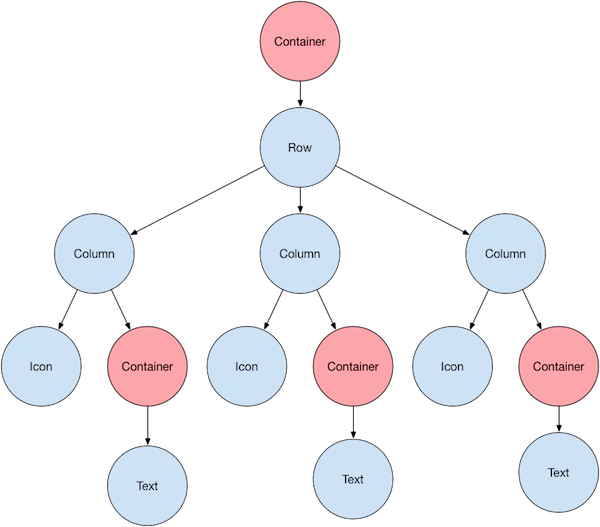
\includegraphics[scale=0.5]{Theoretische_Grundlagen/images/flutter_widget_tree.png}
	\end{center}
	\caption[Widget Baum einer beispielhaften Anwendung]{Widget Baum einer beispielhaften Anwendung \protect \footnotemark}
	\label{fig:flutter_widget_tree}
\end{figure}
\footnotetext{Quelle: \url{https://flutter.dev/docs/development/ui/layout}, letzter Zugriff: 21. März 2021}
	

\paragraph{States}
Flutter ist deklarativ - das bedeutet, die Benutzeroberfläche wird anhand von dem aktuellen \textit{State} der App erzeugt. 
Im Gegensatz dazu muss der Entwickler beim imperativen Stil die Übergänge der einzelnen \textit{States}. 
Die Abbildung \ref{fig:flutter_state} stellt eine deklarative Benutzeroberfläche dar. 
Hier wird dies durch das Framework gelöst. 
	
\begin{figure}[tbt]
	\begin{center}
		
\includegraphics[scale=0.4]{Theoretische_Grundlagen/images/flutter_state.png}
	\end{center}
	\caption[Deklarative Benutzeroberfläche]{Deklarative Benutzeroberfläche \protect \footnotemark}
	\label{fig:flutter_state}
\end{figure}
\footnotetext{Quelle: \url{https://flutter.dev/docs/development/data-and-backend/state-mgmt/declarative}, letzter Zugriff: 12. April 2021}








\subsection{Recommender System}
\label{sec:recomandationSystem}
Auf der Webseite Youtube allein werden minütlich mehr als 500 Stunden Videomaterial hochgeladen. (\url{https://blog.youtube/press/}, 10.02.2021)
Um bei einer solch unvorstellbaren Menge an Daten (allein auf einer Webseite) den Überblick als Endnutzer behalten zu können, ist ein personalisierten Filtersystems unausweichlich.

\noindent
Solche Filtersysteme, auch Recommendation System genannt, nutzt bisher gesammelte Daten um Nutzern potentiell interessante Objekte jeweils individuell vorzuschlagen.
Ein sogenannter \textit{Candidate Generator} ist hierbei ein Recommendation System, welches die Menge $M$ als Eingabe erhält und für jeden Nutzer eine Menge $N$ ausgibt. Hierbei umfasst $M$ alle Objekte und gleichzeitig gilt $N \subset M$. 

\noindent
Die Bestimmung einer solchen Menge $N$ beruht grundlegend auf zwei Informationsarten. Erstens die sogenannten Nutzer-Objekt Interaktionen, also beispielsweise Bewertungen oder auch Verhaltensmuster; Und zweitens die Attributwerte von jeweils Nutzer oder Item, also beispielsweise Vorlieben von Nutzern oder Eigenschaften von Items.\cite{aggarwal2016}
Systeme, welche zum Bewerten ersteres benutzen, werden \textit{collaborative filtering} Modelle genannt. Andere, welche zweiteres verwenden, werden \textit{content-based filtering} Modelle genannt. Wichtig hierbei ist jedoch, dass \textit{content-based filtering} Modelle ebenfalls Nutzer-Objekt Interaktionen (v.a. Bewertungen) verwenden können, jedoch bezieht sich dieses Modell nur auf einzelne Nutzer - \textit{collaborative filtering} basiert auf Verhaltensmustern von allen Nutzern bzw. allen Objekten.

\noindent
Ein solches Recommendation System kann im einfachsten Fall wie in \ref{Recommendation Matrix} als Matrix dargestellt werden.

\begin{table}[tbt]
	\caption{Nutzer-Item Matrix mit Bewertungen. Jede Zelle $r_{u;i}$ steht hierbei für die Bewertung des Nutzers $u$ an der Stelle $i$}
	\centering
	\label{Recommendation Matrix}
	\begin{tabular}{lcllllll}
		& \multicolumn{7}{c}{Items}                                                                                                                                                        \\
		& \multicolumn{1}{l}{}     & \multicolumn{1}{c}{1}  & \multicolumn{1}{c}{2}  & \multicolumn{1}{c}{...} & \multicolumn{1}{c}{i}  & \multicolumn{1}{c}{...} & \multicolumn{1}{c}{m}  \\ \cline{3-8} 
		& \multicolumn{1}{c|}{1}   & \multicolumn{1}{l|}{2} & \multicolumn{1}{l|}{}  & \multicolumn{1}{l|}{1}  & \multicolumn{1}{l|}{}  & \multicolumn{1}{l|}{}   & \multicolumn{1}{l|}{3} \\ \cline{3-8} 
		Users & \multicolumn{1}{c|}{2}   & \multicolumn{1}{l|}{4} & \multicolumn{1}{l|}{}  & \multicolumn{1}{l|}{}   & \multicolumn{1}{l|}{5} & \multicolumn{1}{l|}{}   & \multicolumn{1}{l|}{}  \\ \cline{3-8} 
		& \multicolumn{1}{c|}{...} & \multicolumn{1}{l|}{}  & \multicolumn{1}{l|}{}  & \multicolumn{1}{l|}{1}  & \multicolumn{1}{l|}{}  & \multicolumn{1}{l|}{}   & \multicolumn{1}{l|}{4} \\ \cline{3-8} 
		& \multicolumn{1}{c|}{u}   & \multicolumn{1}{l|}{}  & \multicolumn{1}{l|}{4} & \multicolumn{1}{l|}{}   & \multicolumn{1}{l|}{5} & \multicolumn{1}{l|}{}   & \multicolumn{1}{l|}{1} \\ \cline{3-8} 
		& \multicolumn{1}{l|}{}    & \multicolumn{1}{l|}{2} & \multicolumn{1}{l|}{}  & \multicolumn{1}{l|}{}   & \multicolumn{1}{l|}{}  & \multicolumn{1}{l|}{3}  & \multicolumn{1}{l|}{}  \\ \cline{3-8} 
		& \multicolumn{1}{l|}{n}   & \multicolumn{1}{l|}{}  & \multicolumn{1}{l|}{4} & \multicolumn{1}{l|}{}   & \multicolumn{1}{l|}{3} & \multicolumn{1}{l|}{}   & \multicolumn{1}{l|}{}  \\ \cline{3-8} 
	\end{tabular}
\end{table}

\subsubsection{Nutzerinformation}
Damit ein \textit{Recommender System} einem Nutzer Vorschläge bereitstellen kann, benötigt es Nutzerinformationen. Das Design des jeweiligen Systems hängt auch, wie oben beschrieben, von der Art der Information und von der Art der Beschaffung dieser ab.

\paragraph{Explizite Nutzerinformation}
Bei der expliziten Methode muss der Nutzer individuelle Informationen aktiv über sich preisgeben. Dies kann über konkrete Fragestellungen zu beispielsweise Geburtsdatum, Geschlecht oder Interessen geschehen. Diese Art der Information beschreiben einen Nutzer konkret. 

\noindent
Eine andere Art der Information sind Bewertungen von Objekten. Diese lassen sich beispielsweise Intervall basiert darstellen. Hierbei werden geordnete Zahlen in einem Intervall als Indikator genutzt, ob ein Objekt gut oder schlecht war - zum Beispiel eine Bewertung eines Produktes von 0 bis 5 Sternen bei Amazon. Diese Information beschreiben die Vorlieben eines Nutzers konkret.

\noindent
Je größer diese Skala ist, desto differenzierter ist auch das Meinungsbild, da jeder Nutzer sich genau ausdrücken kann. Jedoch desto komplizierter und unübersichtlich wird auch das Bewertungsverfahren an sich, da man einen zu großen Entscheidungsraum für den Nutzer darbietet.

\paragraph{Implizite Nutzerinformation}
Um implizit Nutzerinformationen zu erfassen, muss ein System die Verhaltensmuster seiner Kunden als Daten abspeichern. Beispielsweise könnte das System von YouTube erfassen, ob Videos frühzeitig abgebrochen oder ganz angeschaut werden. Anklicken von Webseiten und die darauf verbrachte Zeit könnte ebenfalls als Bewertung gespeichert und zur Generierung von Vorschlägen genutzt werden.

\subsubsection{Content-based filtering}
Unter \textit{content-based filtering} versteht man das Betrachten von Ähnlichkeiten zwischen Objekten anhand von Schlüsselwörtern (Eigenschaften) und daraus dann das Vorhersagen der Nutzer-Objekt Kombination für ein bestimmtes Objekt. 
Nimmt man an, Film 1 und Film 2 haben ähnliche Eigenschaften (gleiches Genre, gleiche Schauspieler, ...) und Nutzer A mag Film 1, so wird das System Film 2 vorschlagen.

\noindent
Das System ist also unabhängig von anderen Nutzerdaten, da die Vorschläge nur auf Präferenzen eines einzelnen Nutzers basieren. Dies bietet im Hinblick auf eine App auch gute Skalierungs"-möglich"-keiten. Zudem kann auf Nischen-Präferenzen gut eingegangen werden, da nicht mit anderen Nutzerdaten verglichen wird, sondern nur ein Nutzer für sich betrachtet wird.

\noindent
Gleichzeitig schlagen \textit{content-based filtering} Systeme aber eher offensichtliche Objekte vor, da Nutzer oft unzureichend genaue "Beschreibungen", also Vorlieben mit sich bringen. Dadurch, dass nur basierend auf Schlüsselwörter neue Objekte vorgeschlagen und andere Nutzerwertungen nicht miteinbezogen werden, sind die Vorschläge sehr wahrscheinlich oftmals ähnlich bis gleich - man "verfängt" sich quasi in eine Richtung.\cite{aggarwal2016}

\subsubsection{Collaborative Filtering}
Unter \textit{collaborative filtering} versteht man das Betrachten von Ähnlichkeiten im Verhalten von Nutzern anhand von Bewertungen und Prä"-fer"-enzen, bzw. anhand der Ähn"-lich"-keiten von Objekten.

\noindent
Generell unterscheidet man in zwei Typen:\cite{aggarwal2016}

\begin{enumerate}		
	\item \textit{Memory-based Methoden}: Es wird, wie oben beschrieben, aus gesammelten Daten Ähn"-lich"-keit herausgearbeitet und Nutzer-Objekt Kombinationen durch eben diese vorhergesagt. Daher wird dieser Typ auch \textit{neighborhood-based collaborative filtering} genannt. Man unterscheidet weiter in:
	\begin{enumerate}
		\item \textit{User-based}: Ausgehend von einem Nutzer A werden andere Nutzer mit ähnlichen Nutzer-Objekt Kombinationen gesucht, um Vorhersagen für Bewertungen von A zu treffen. Ähnlichkeitsbeziehungen werden also über die Reihen der Bewertungsmatrix berechnet.
		\item \textit{Item-based}: Hierbei werden ähnliche Objekte gesucht und diese genutzt um die Bewertung eines Nutzers für ein Objekt vorherzusagen. Es werden somit Spalten für die Berechnung der Ähnlichkeitsbeziehungen verwendet.
	\end{enumerate}
	\item \textit{Model-based Methoden}: Machine Learning und Data Mining Methoden werden verwendet um Vorhersagen über Nutzer-Objekt Kombinationen zu treffen. Hierbei sind auch gute Vorhersagen bei niedriger Bewertungsdichte in der Matrix möglich.
\end{enumerate}

\noindent
Vereinfacht gesagt: Wenn Nutzer A ähnliche Bewertungen verteilt wie Nutzer B, und B den Film 1 positiv bewertet hat, wird das System Film 1 auch Nutzer A vorschlagen. Das selbe gilt auch umgekehrt (\textit{Item-based}).

\noindent
Diese Art leidet sehr unter dem \textit{sparsity} Problem, also dass die Nutzer zu wenige Bewertungen von Objekten ausüben. Daher sind Vorhersagen über Ähnlichkeit von Nutzern aufgrund unzureichender Datensätze nicht sinnvoll möglich. Dieses Problem wird \textit{Cold-Start Problem} genannt.

\subsubsection{Ähnlichkeit von Objekten und Nutzern}
Sowohl bei \textit{collaborative filtering}, als auch bei \textit{content-based filtering} wird jedes Objekt und jeder Nutzer als ein Vektor im Vektorraum-Modell $E = \mathbb{R}^d$ (englisch \textit{embedding space}) erfasst. Sind Objekte beispielsweise ähnlich, haben sie eine geringe Distanz voneinander. 

\noindent
Ähnlichkeitsfunktionen sind Funktionen $s : E \times E  \rightarrow \mathbb{R}$ welche aus zwei Vektoren beispielsweise von einem Objekt $q \in E$ und einem Nutzer $x \in E$ ein Skalar berechnen, welches die Ähnlichkeit dieser zwei beschreibt $s(q,x)$.

\noindent
Hierfür werden mindestens eine der folgenden Funktionen verwendet:
\begin{itemize}
	\item Cosinus-Funktion
	\item Skalarprodukt
	\item Euklidischer Abstand
\end{itemize} 

\paragraph{Cosinus-Funktion}
Hier wird einfach der Winkel zwischen beiden Vektoren berechnet: $s(q,x) = \cos(q,x)$

\paragraph{Skalarprodukt}
Je größer das Skalarprodukt, desto ähnlicher sind sich die Vektoren. $s(q,x) = q \circ x = \sum_{i=1}^{d}q_i x_i$ 

\paragraph{Euklidischer Abstand}
$s(q,x) = ||q-x|| = [\sum_{i=1}^{d}(q_i - x_i)^2]^\frac{1}{2}$





\url{https://dl.acm.org/doi/pdf/10.1145/3383313.3412488}
\url{http://www.microlinkcolleges.net/elib/files/undergraduate/Photography/504703.pdf}

% Neue Section, neue Seite
\clearpage
\section{Planung}
\label{sec:app_concept}
%TODO Section{Idee/Gedankengänge/Planung} in der \subsectino{Konzept} mit den Wünschen des Users und die Benötigten Ressourcen und eine subsection{Komponenten} mit Unseren Komponenten/Ressourcen und wie sie miteinander funktionieren.

\subsection{Konzept}
Aus Perspektive der Benutzer ist die Idee hinter StreamSwipe trivial. Dem User werden nacheinander Filme und Serien vorgeschlagen, die er bewerten kann. Auf Basis seiner Präferenzen erhält er Matches, mit denen er über sich eine Chatfunktionen austauschen kann. Jeder dieser Schritte muss möglichst schnell und unkompliziert erfolgen.\\
Aus Sicht des Anbieters ist die Realisierung wesentlich komplexer als es dem User erscheint, da eine Zusammenstellung an Komponenten benötigt wird.  Diese besteht aus einer Smartphone-App, einer Userdatenbank, einer Datenbank mit den Filminformationen und einem Server, der das Matching ausführt. Zusätzlich wird eine mögliche Komponente für den Messenger benötigt. Die Auswahl dieser Komponente wird jeweils über individuell gestellte Anforderungen getroffen. \\

\noindent
Bei der Smartphone-App muss bereits während der Entwicklung auf Benutzerfreundlichkeit und Barrierefreiheit geachtet werden. Sie sollte intuitiv bedienbar, attraktiv designt und ressourcensparend für leistungsschwache Smartphones programmiert sein. Um ein möglichst großes Publikum ansprechen zu können, muss sie für iOS und Android erhältlich sein.\\
Die Datenbank mit den Benutzerinformationen muss jederzeit erreichbar sein und eine gewisse Form von Sicherheit und Verschlüsselung bieten, da da hier persönliche Angaben gespeichert werden.\\
Die Datenbank mit den Filminformationen  muss sehr umfangreich sein, also auch ältere Filme und Nischenfilme enthalten, und ständig aktualisiert werden. Neben den offensichtlichen Informationen wie Filmtitel und Filmposter muss sie auch weitere Daten zu den Filmen enthalten wie Erscheinungsdatum, Handlung, Regie, etc. trotzdem sollte der Zugriff schnell sein und nichts kosten, sodass die Nutzung der App möglichst preiswert ist.\\
Der Server muss durchgehend laufen und über eine Internetverbindung erreichbar sein. Er muss leistungsstark genug sein um alle Nutzeranfragen bedienen zu können, sollte jedoch so klein gehalten werden, dass die Anschaffungs- und Unterhaltskosten minimal sind.\\
Der Messenger  muss ebenfalls über einen zentralen Punkt gesteuert werden, da sich nur zwischen Personen ein Chat öffnen darf, die gematcht wurden. Es sollte keine Zugriffsbegrenzung auf diesen Server  geben, um einen unbegrenzten  Nachrichtenwechsel garantieren zu können. Nachrichten müssen gespeichert werden, um versendete Nachrichten auch nach dem Schließen der App zustellen zu können. Das System muss ebenfalls verschlüsselt sein und benötigt Zugriff auf Benutzerinformationen wie ID, Name und Profilbild.



X Server muss ständig laufen/erreichbar sein und Internetverbindung haben. In diesem Fall ein Raspberry Pi mit ... was eigentlich??? \\ %TODO Kapitel lesen!!!



\subsection{Komponenten}
\label{sec:komponenten}
In StreamSwipe ist für jede dieser Komponenten eine Lösung gefunden worden.
Bei der Entwicklung der App wurden Benutzerfreundlichkeit und Barrierefreiheit beachtet, wie in Abschnitt \ref{sec:UI-allgemein}, bzw. Abschnitt \ref{sec:barrierefreiheit} gezeigt wird. Wie in Abschnitt \ref{sec:framework} beschrieben wird, können die genannten Anforderungen durch eine geschickte Wahl des Frameworks erfüllt werden. Als Benutzerdatenbank kann Firebase verwendet werden, da wie in Abschnitt \ref{sec:firebase} beschrieben, die benötigten Funktionen vorhanden sind. Es ist ebenfalls möglich den Messenger mit den Firebasefunktionen zu implementieren. Als Quelle der Filminformationen wird die API von \glqq The Movie Database\grqq \, (TMDb) verwendet, auf welche in Abschnitt \ref{sec:filmdatenbank} genauer eingegangen wird. Der verwendete Server besteht aus einem Raspberry Pi, jedoch mehr dazu in Kapitel \ref{sec:server}. Wie diese Komponenten aufeinander zugreifen wird in Abbildung \ref{fig:komponentendiagramm} verdeutlicht.\\
Über die Smartphone-App werden die Benutzerdaten an Firebase weitergeleitet. Wird ein neuer Account angelegt, so werden diese Daten dort gespeichert und bei einem Anmeldevorgang sie mit den bestehenden Benutzerdaten verglichen. Nur wenn der User bereits vorhanden ist, kann eine Anmeldung stattfinden. So wird sichergestellt, dass nur angemeldete Benutzer auf die eigentlichen Funktionen der App Zugriff erhalten. Jede Aktion in der App wird auf diese Weise einem Benutzerkonto zugewiesen und kann später darüber identifiziert werden. Innerhalb der App können alle Funktionen frei genutzt werden weshalb es wichtig ist, dass ausschließlich eingeloggte User auf die Screens der App zugreifen können.\\
Der Server erhält die Film-IDs aller Filme aus der TMDb-API  und erstellt somit eine eigene Film-Datenbank. Diese IDs werden an das Smartphone weitergeleitet und die App erhält über die IDs die Filminformationen direkt von der TMDb-API. Es werden gleichzeitig nur eine geringe Anzahl an Filminformationen aus der TMDb-API auf das Smartphone geladen, sodass dieser Vorgang möglichst wenig Ressourcen benötigt und unbemerkt im Hintergrund ablaufen kann. Hierzu zählen Filmposter, Rating, Besetzung, Veröffentlichungsdatum, übersetzte Sprachen und viele mehr, die teilweise nicht benötigt werden. Noch bevor der User über alle diese Filme abgestimmt hat, werden neue Filminformationen geladen, sodass es für den User keine Unterbrechungen gibt und es ihm wie ein einzelner unendlicher Fluss an Daten erscheint. \\
Die Filmbewertung wird mit den Film-IDs vom Smartphone an den Server geschickt, der diese beiden Informationen miteinander verknüpft. Das Rekommendationsverfahren auf dem Server verarbeitet diese Präferenzen und sucht wie in Kapitel \ref{sec:recomandationSystem} beschrieben nach Übereinstimmungen bei den anderen Benutzern. Da hierbei alle Präferenzen aller User miteinander verglichen werden, ist dieser Schritt sehr aufwändig und sollte nicht nach jeder neuen Präferenz durchgeführt werden. Bei StreamSwipe wird dieses Matching deshalb automatisch in regelmäßigen Zeitabständen durchgeführt, optimalerweise zu einer Tageszeit, an der die Benutzeraktivität gering ist. Die Anzahl der verglichenen Nutzer kann mit einer Filterung durch Geschlechterpräferenzen und Wohnort reduziert werden um das Matchingverfahren zu beschleunigen. \\
Werden zwei User gematcht, wird dies ihnen jeweils in der App angezeigt. Die beiden Benutzer können dann einzeln entscheiden, ob sie die Unterhaltung starten wollen. Ist dies der Fall, werden die Nachrichten in der Firebase-Datenbank gespeichert. %TODO hier die abläufe des chats abklären!!!



%TODO Auch Leon fragen wie exakt das ganze abläuft
- Der Messenger kann ebenfalls über Firebase realisiert werden\\ %TODO Inwieweit gibts hier ein Kapitel drüber?

- Nutzer ID von beiden Nutzern bekannt bei der  Erstllung eines Chats
- Aus diesen beiden wird eine unique ID für den jeweiligen Chat erstellt und diese wird bei beiden Usern gespeichert
- (Firebase ist hierarchisch aufgebaut) Nutzernamen, NutzerID und RoomID werden in einer Sammlung gespeichert. Unter dieser Sammlung werden dann die Nachrichten abgespeichert mit den Informationen Wers gesendet hat, wers empfängt, einen tmestamp und natürlcih den inhalt der nachricht. sendby und sendto werden verwendet um die nachrichten im Chatverlauf anzuordnen und zu entscheiden welcher der beiden beteiligten eine benachrichtigung bekommt
- Anzeige der Chats abhängig davon ob die uniqueID in chatrooms oder pendingchatrooms gespeichert ist
- Wer die unterhaltung beginnt, erhält die unique ID in chatrooms und der andere in pendingchatrooms
- NImmt der andere User den Chat an, wird die ID für ihn ebenfalls in chtarooms verschioben
-


\begin{figure}[h]
\centering
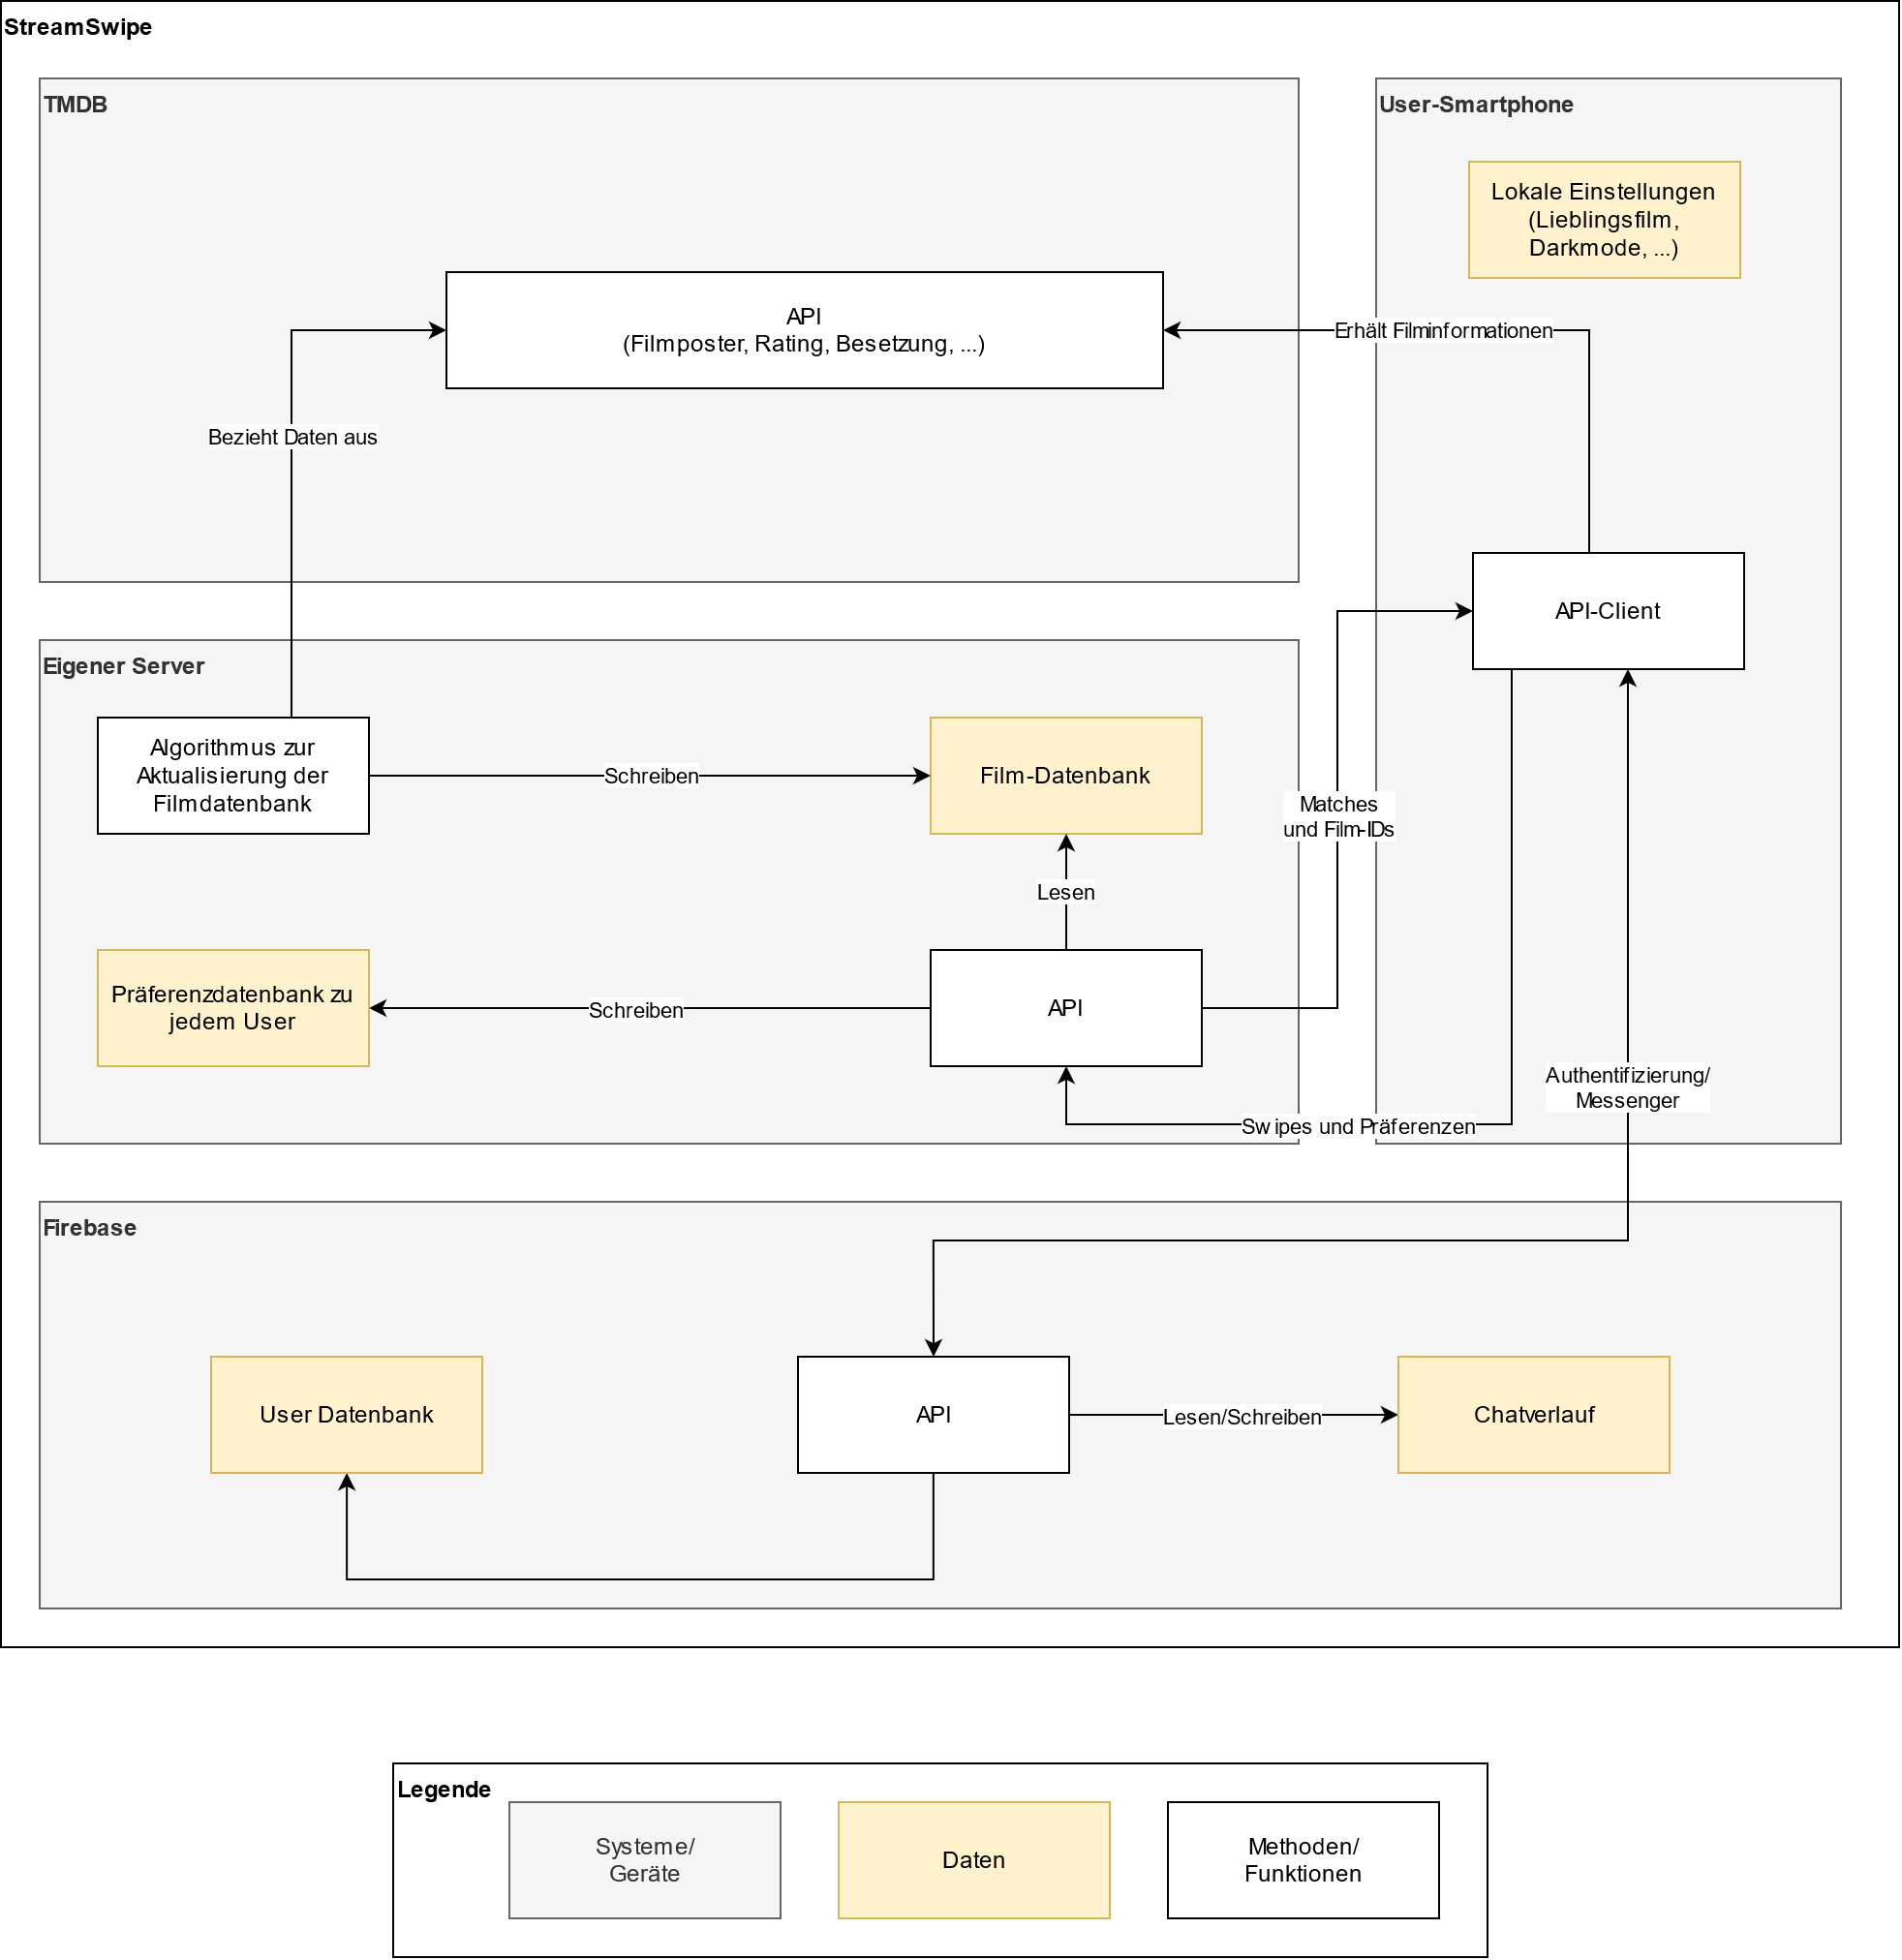
\includegraphics[width=16cm]{images/Konzeptdiagramm.png}
\caption{Komponentendiagramm}
\label{fig:komponentendiagramm}
\end{figure}


% Neue Section, neue Seite
\clearpage
\section{Auswahl geeigneter Technologie}
Den Anforderungen der Entwicklung entsprechend wurde zunächst entschieden, welche Technologien zum Einsatz kommen. 

\subsection{Anwendungsframework}
Bei der Auswahl des Framework zur Programmierung der eigentlichen Anwendung gibt es, wie in Kapitel \ref{sec:mobile_development} erläutert, eine Vielzahl von möglichen Herangehensweisen.
Die Anwendung ist letztendlich der Teil unseres Systems, welches direkt mit dem Nutzer in Berührung kommt.
Daher sind vor allem die Anforderungen an Performance, Aussehen und Benutzbarkeit der Oberfläche essentiell wichtig.
Gleichzeitig ist bei der Entwicklung auf die verwendete Programmiersprache, die Entwicklungsumgebung, welche das Framework mit sich bringt und die Kenntnisse aller Entwickler zu achten.\\
\\
Wie bereits in Abbildung \ref{fig:crossplattform_popularity} gezeigt, können sich Marktanteile verschiedener Frameworks sehr schnell ändern. 
Dies hängt auch deutlich mit den unterliegenden Plattformen und deren Update-Zyklen zusammen.
Google beispielsweise veröffentlicht beinahe jährlich eine neue Version von Android\footnote{\url{https://engineerbabu.com/blog/evolution-of-android-versions/}, letzter Zugriff: 20. April 2021}, weshalb sich eben Programmierumgebungen immer mitentwickeln.
Die Popularität eines Frameworks spiegelt somit unter anderem wieder, wie gut es mit den neuesten Features und Programmierkonzepten umgeht. 
Daher wurde sich bei den plattformübergreifenden Frameworks \ref{sec:framework} auf React Native und Flutter beschränkt. 
Beide bieten vordefinierte, nativ implementierte Benutzeroberflächenkomponenten - welche im Falle von Flutter sogar auf dem Design System \href{https://material.io/}{\textit{Material Design}} beruht.\\
Das Konzept aus Kapitel \ref{sec:app_concept} schlägt vor, dem Nutzer die Bewertung einzelner Filme über eine Wisch-Funktion bereitzustellen.
Allein dieser Bildschirm muss zunächst einmal eine Reihe von Filmen inklusive Titelbild und Informationen über HTTP Anfragen von unserer Datenbank laden, die Animationen und Logik hinter dem Bewertungssystem abarbeiten und zusätzlich die Bewertung wieder zurück an unseren Server senden.
Aufgrund dieses enorm hohen Performance-Anspruchs sind nativ implementierte Komponente unabdingbar.
Da sowohl Flutter als auch React Native es ermöglichen, die UI Komponenten in der plattformspezifischen Sprache zu implementieren, erweist sich der Leistungsvergleich beider Frameworks als schwierig.
Grundlegend kann jedoch angenommen werden, dass Flutter eher weniger CPU-Nutzung beansprucht, jedoch dazu tendiert, mehr Speicher vor der eigentlichen Anwendung anzufordern \cite{bjorn-hansen2020}.

Somit kristallisierten sich drei Entwicklungsmöglichkeiten per Ausschlussverfahren heraus:
\begin{itemize}
	\item Native Anwendung für jeweils Android und iOS
	\item Plattformübergreifend mit Flutter
	\item Plattformübergreifend mit React Native
\end{itemize}

Mit einer nativen Anwendung für jede Plattform erhält man nicht nur doppelten Entwicklungsaufwand, sondern gleichzeitig auch doppelten Wartungsaufwand. 
Zusätzlich gegen die native Möglichkeit spricht, dass für die Entwicklung einer iOS Anwendung die Entwicklungsumgebung XCode benötigt wird, welche eine Desktopanwendung ausschließlich für das Betriebssystem macOS ist.
Daher ist die Entwicklung nicht nur in Sachen Codezeilen ein deutlicher Mehraufwand, welcher sich aber bei der Größe des Projektes nicht bezahlt macht.
Bei den plattformübergreifenden Lösungen entfällt dieser Aspekt, jedoch ist das veröffentlichen einer iOS Anwendung im Vergleich zu Android weiterhin deutlich komplizierter - hierauf wird im weiteren Verlauf der Arbeit noch eingegangen.\\
\\
Beim direkten Vergleich zwischen React Native und Flutter ist der deutlichste Unterschied, dass React Native die Entwicklung einer Laufzeit-basierten Anwendung bietet und Flutter die einer kompilierten Anwendung.
Hierbei werden unterschiedliche Programmiersprachen verwendet: Flutter beruht auf der Google eigenen Sprache Dart. 
Da diese sich bisher noch nicht etablieren konnte, ist diese Sprache unbekannt und muss neu erlernt werden.
JavaScript hingegen ist weit verbreitet, jedoch bringt die spezielle Erweiterung JSX bei React Native ebenfalls zusätzlichen Lernaufwand mit sich.\\
Während der Entwicklung bieten beide Frameworks eine \glqq Hot Reload\grqq Funktion an, welche vor allem bei der Erstellung von Benutzeroberflächen deutliche Zeitersparnisse ermöglicht.
Flutter punktet jedoch vor allem hierbei durch die direkte Unterstützung von UI Bibliotheken, welche React Native ausschließlich über externe Bibliotheken bezieht. 
Gleichzeitig bringt Flutter allgemein mehr \glqq out of the box\grqq mit sich, weshalb bei React Native eher Probleme durch Abhängigkeiten von Drittanbieter entstehen können. \\
\\
Der ausschlaggebende Punkt ist jedoch tatsächlich die BaaS-Plattform (Backend-as-a-Service).
Es existiert zwar ein großer Konkurrent zu Firebase, nämlich \href{https://docs.amplify.aws/}{AWS Amplify}.
Hierbei handelt es sich ebenfalls um ein Backend-Service für Mobil- und Webanwendungen. 
Aufgrund der auf Skalierung ausgesetzten Tools mit besseren Echtzeit-Features ist Firebase jedoch speziell für Nachrichtenaustausch besser geeignet.
Gleichzeitig spielt die Vertrautheit mit dieser BaaS Plattform und die breit gefächerten Tools eine große Rolle bei der Auswahl des Services.
Letztendlich wurde die Entscheidung getroffen, das allgemeines Nutzermanagement und Chat-Funktion der Anwendung mit Firebase zu realisieren.\\
Da AWS Amplify erst seit Beginn 2021 eine offizielle Unterstützung für Flutter anbieten\footnote{\url{https://aws.amazon.com/de/about-aws/whats-new/2021/02/announcing-general-availability-amplify-flutter-data-authentication-support/}}, wurde Flutter als Frontend-Framework und Firebase als BaaS-Plattform ausgewählt.

\subsection{Server}
\label{sec:server}
Der Webserver ist jener Dienst,  der die zugrundeliegenden Funktionalitäten bezüglich der Filmabfragen, der Matching-Logik und der Filmempfehlung bietet. 
Anforderungen an die genutzte Webservertechnologie sind zum einen eine grundlegend hohe Performance, um mit einer hohen Anzahl an Serveranfragen umzugehen. Des Weiteren sollte die Technologie Skalierbarkeit in Bezug auf die Performance und wachsenden Ressourcen wie Hardware aufweisen und eine Unterstützung, Dokumentation und umfassende Funktionalitäten des Frameworks bieten. 
Ein Paketmanager, der umfassende Kern-Funktionalitäten zur Verfügung stellt, sollte vorhanden sein, damit diese nicht neu implementiert werden müssen. Um offen für das genutzte Zielbetriebssystem zu bleiben, sollten mehrere Betriebssysteme unterstützt werden. 
Im folgenden werden keine proprietären Webserver-technologien betrachtet.
\newline
Nach genauerer Recherche kamen drei Webservertechnologien in die engere Betrachtung:

\begin{itemize}
	\item PHP
	\item Django
	\item Node.js
\end{itemize} 

\noindent
Im Hinblick auf die Performance sticht Node.js aufgrund seiner ereignisgesteuerter Architektur  und dem Non-Blocking I/O-Mechanismus heraus und verspricht eine bessere Ressourcennutzung. 
\newline
Große Firmen wie Uber \footnote{siehe \url{https://eng.uber.com/uber-tech-stack-part-two/ }, letzter Zugriff: 18. März 2021}, Ebay und Netflix \footnote{siehe \url{https://entwickler.de/online/javascript/7-gruende-node-js-579924149.html}, letzter Zugriff: 18. März 2021 } haben ihre Systeme bereits auf Node.js umgestellt. Die Wahl als Webservertechnologie fällt auf Node.js, da es breite Unterstützung erfährt, die auch durch den mächtigen Paketmanager npm ergänzt wird und eine hohe Performance errichtet.


\subsection{Datenbank}
Im Hinblick auf die Speicherung der potenziell hohen Anzahl an Nutzern, deren Swipe-Ent\-schei\-dungen und deren Matches untereinander sowie der Anzahl von über 500.000 Filmen\footnote{siehe \url{https://www.themoviedb.org/faq/general}, letzter Zugriff: 18. März 2021} wird ein performanter Umgang der Datenbank mit vielen Datensätzen notwendig sein.  
Um massive Daten speichern zu können sind relationale Datenbanken nicht die passende Wahl. 
Es hat sich gezeigt, dass je größer die Menge an Daten ist und je mehr Tabellen in einer Anfrage enthalten sind, desto größer ist der Performanceverlust durch SQL. \cite{4.5}
\newline
Die Verwendung von dokumentenbasierten Datenbanken führt dagegen zu einer strukturlosen Zusammensetzung an Daten, bei denen ein Dokument ein einzelnes Objekt repräsentieren kann. 
Somit muss für die Wiedergabe eines Objekts nur ein Dokument angefragt werden. Die fehlenden Möglichkeiten zur Normalisierung können jedoch zu Redundanzen in den Daten führen, wodurch die Entwicklung der aufrufenden Anwendung komplexer werden kann. 
Die Redundanz wird jedoch in Kauf genommen, um schnelle Abfragen zu ermöglichen und eine hohe Performance zu erhalten. Da Datensätze in dokumentenbasierten NoSQL-Datenbanken schemalos als JSON-Objekte abgelegt werden, begünstigt dies den generischen Dokumentenaufbau in der Entwicklung.
\newline
Einige NoSQL-Datenbanken wie MongoDB verfolgen einen nicht-relationalen Ansatz und werden mit JavaScript-fähigen Schnittstellen bereitgestellt. Durch die Kommunikation im JSON-Format eignen ist ein optimaler Einsatz mit Node.js gegeben. MongoDB ist über seine horizontale Skalierbarkeit darauf ausgelegt, in einem kurzen Zeitraum sehr viele Daten zu verarbeiten \cite{Tech6}. Während relationale Systeme vertikal im Sinne von neuen Tabelleneinträgen skalieren, werden Dokumente hingegen werden in einer Kollektion, die horizontal erweitert werden können, indem Datenmengen im Sinne des Shardings auf mehreren Systemen verteilt werden, anstatt ein einzelnes System zu verwenden.
\newline
Als Datenbank für die Backend-Implementierung wurde aufgrund von Performance, der guten Einbindung an Node.js und der Skalierbarkeit MongoDB ausgewählt. Um die Vorteile der Da\-ten\-kompression sowie der Transaktionen über mehrere Dokumente hinweg zu nutzen, ist die WiredTiger-Engine die Wahl für das genutzte Storage-Engine.  


\subsection{Kommunikationsschnittstelle}
Als Kommunikationsschnittstelle wird eine WebApi entwickelt, dessen Kommunikation auf HTTP-Nachrichten basiert, deren Informationen im JSON-Format übergeben werden. Diese Technologie bietet eine einfache und dennoch effiziente Form der Kommunikation zwischen Server und Client.

\subsection{Film-Datenbank}
\label{sec:filmdatenbank}
Um die Informationen der einzelnen Filme anzeigen zu können, werden zunächst einmal Informationen benötigt.
Hierfür existieren mehrere Anbieter, wobei die Anbindungen und auch die Datensätze selbst von unterschiedlicher Qualität sind.\\
\\
Für die API der OMDb (Open Movie Database) ist leider keine gute Dokumentation frei verfügbar.
Gleichzeitig ist der Zugriff über 1000 Anfragen pro Tag und eine Poster API zur Anzeige der Filmposter nur verfügbar, falls man eine Spende über Patreon hinterlässt\footnote{Quelle: \url{https://www.omdbapi.com/}, letzter Zugriff: 20. März 2021}.\\
\\
Die API von IMDb (Internet Movie Database) ist hingegen sehr gut dokumentiert und bietet auch die wichtigsten Daten (Titel, Beschreibung und Bild) an.
Problem hieran ist jedoch, dass es zwar einen kostenlosen Zugang gibt, dieser jedoch auf 100 Anfragen täglich beschränkt ist\footnote{Quelle: \url{https://imdb-api.com/}, letzter Zugriff: 20. März 2021}. 
Gleichzeitig hat diese API eine Verzögerung von knapp 1\,s, was zu schlechter Benutzererfahrung führen kann\footnote{Quelle: \url{https://rapidapi.com/amrelrafie/api/movies-tvshows-data-imdb}, letzter Zugriff: 20. März 2021}.\\
\\
Letztendlich wurde die Version 3 der API von TMDb (The Movie Database) gewählt.
Sie ist außerordentlich gut dokumentiert und bietet mehr Möglichkeiten als für diese Anwendung überhaupt notwendig.
Beispielsweise lassen sich Filme bewerten, nach Genre Filme suchen oder auch Trailer anzeigen.
Sie ist gratis für jeden zur Nutzung verfügbar, solange in der Anwendung angegeben ist, dass diese Film-Datenbank verwendet wurde.
Die Nutzung wiederum ist unbegrenzt, also es existiert keine Abfragenlimitierung\footnote{Quelle: \url{https://developers.themoviedb.org/3/}, letzter Zugriff: 20. März 2021}.


% Neue Section, neue Seite
\clearpage
\section{Serverseitige Implementierung}
Unter dem Begriff "Backend" versteht man Komponenten eines digitalen Systems, die den Betrieb des Programms ermöglichen und vom Benutzer nicht ersichtlich sind.
\newline
Eine Backend-Anwendung kann direkt mit dem Frontend interagieren und dessen Benutzerdienste unterstützen sowie die Schnittstellen mit allen erforderlichen Ressourcen anbieten.

\subsection{Datenbank}
Hier steht mein BackendDatenbank Text.

\subsubsection{Einrichtung}
Hier steht mein Imlementierung Text.

\subsection{StreamSwipe-Webserver}
Hier steht mein BackendServer Text.

\subsubsection{Einrichtung}
Zunächst...


\subsubsection{Sicherheit}
Den Server gilt es zu schützen.

\subsubsection{Webserver}
Den Server gilt es zu schützen.



\subsection{Firebase}
\label{sec:implementierung_firebase}
Firebase bietet viele verschiedene Werkzeuge zur Entwicklung und Überwachung von Mobil- und Webanwendungen.
Nach dem Konzept nach Kapitel \ref{sec:concept} beschränkt sich der Aufgabenbereich des Firebase Backends auf Nutzerauthentifizierung, Verwaltung der Nutzerdaten und der Chatfunktion.
Die hierfür genutzten Werkzeuge werden im Folgenden besprochen.\\
Grundlegend muss zunächst eine Anwendung erstellt, ein Firebase Projekt aufgesetzt und diese zusammen verknüpft werden.
Sobald dieser Prozess abgeschlossen ist, muss sichergestellt sein, dass Firebase in der Anwendung initialisiert wird.

\subsubsection{Authentifizierung}
Um Nutzern eine sichere Registrierung, bzw. An- und Abmeldung ermöglichen zu können bietet Firebase das Authentifizierungswerkzeug. 
Dieser Backendservice verfügt über unterschiedliche Authentifizierungsmethoden.
Um es zu nutzen, muss nur die jeweilige Methode ausgewählt werden. \\

\noindent
In unserem Fall wurde die E-Mail und Passwort Authentifizierung gewählt, um unabhängig von Drittanbietern zu sein.
Nun muss das SDK \texttt{firebase\_auth} integriert werden und mithilfe der Funktionen \texttt{createUserWithEmailAndPassword()} bzw. \texttt{signInWithEmailAndPassword()} ein Nutzer registriert und angemeldet werden.
Hierbei können mithilfe von Fehlercodes geeignete Fehlermeldungen erstellt werden. 
Zusätzlich besitzt die Klasse \texttt{User} das Feld \texttt{emailVerified} (Boolean) und die Methode \texttt{sendEmailVerification()}, wodurch eine Verifizierung der E-Mail über Nachrichtenvorlage durchgeführt wird.
Ist ein Nutzer einmal authentifiziert, muss unterschieden werden, welchen Bildschirm er sehen darf.
Hierzu wird darauf geachtet, ob ein aktueller Nutzerobjekt existiert.
Ist dies nicht der Fall, wird der Anmeldebildschirm angezeigt; ansonsten der Hauptbildschirm.
\medspace
\begin{lstlisting}[caption= Anzeige abhängig ob ein aktueller Nutzer existiert]
	// Globale Instanz des Authentifizierungsservice
	final AuthService auth = Provider.of(context).auth;
	return FutureBuilder<User>(
		future: auth.getCurrentUser(),
		builder: (BuildContext context, AsyncSnapshot<User> snapshot) {
			// Existiert ein Nutzer, wird der Hauptbildschirm angezeigt
			if (snapshot.hasData) {
				return MessageHandler();
			} 
			// Zeige ansonsten den Login-Bildschirm
			else {
				return SignUpScreen(authFormType: AuthFormType.signIn);
			}
		}
	);
\end{lstlisting}
\medspace

\subsubsection{Nutzerdaten}
Bei der Authentifizierung eines Nutzers wird mittels des Auth-Services ein Nutzerobjekt erstellt.
Dieses kann folgende Felder besitzen:
\begin{itemize}
	\item Einzigartige Identifikation (UID)
	\item E-Mail Adresse
	\item Namen
	\item Bild-URL
\end{itemize}
Es ist jedoch nicht möglich über diesen Service weitere Eigenschaften abzuspeichern.
Diese müssen über zusätzliche Speicherwerkzeuge, wie beispielsweise Cloud Firestore (siehe \ref{sec:firestore}) gesichert werden.\\
\\
Hierzu wurde die Sammlung \enquote{users} erstellt und bei der Registrierung für jeden Nutzer ein Dokument mit der selben ID, wie die Nutzer UID erstellt. 
Dadurch ist sichergestellt, dass es ein einzigartiges Dokument und der Zugriff einfach geregelt ist.
Hier werden nun weitere Eigenschaften gesichert, welche teilweise ausschließlich zu Anzeigezwecken in Firebase doppelt abgespeichert werden.
\begin{itemize}
	\item Anzeigename
	\item E-Mail
	\item Wohnort, welcher aus den wichtigsten Städten Deutschlands bestehen
	\item Geschlechter, nach welchen gesucht wird
	\item Eigenes Geschlecht
	\item Lieblingsfilm
\end{itemize}
Unser Nutzer jedoch speichert seine Profil und Hintergrundbilder weder im Auth-Service Nutzerobjekt noch im Cloud Firestore Dokument.
Bei Auth-Service lässt sich lediglich die URL zu einem einzigen Bild hinterlegen.
Bei Firestore ist es zwar möglich eine theoretisch unbegrenzte Menge an Bild URLs abzuspeichern, jedoch muss der Nutzer die Möglichkeit haben seine eigenen Bilder hochzuladen und nicht nur eine URL auf ein bereits hochgeladenes Bild abspeichern.\\
\\
Hierfür bietet Firestore das Werkzeug Storage. 
Wie in Kapitel \ref{sec:firebase_storage} beschrieben, können hier Nutzerinhalte hoch- und heruntergeladen werden. 
Dazu wird beim ersten Hochladen ein Ordner für jeden Nutzer erstellt.
Darin werden daraufhin die Bilder unter dem Namen \texttt{profile-picture} oder \texttt{background-picture} jeweils abgespeichert und eventuell überschrieben.
Mit einer Funktion kann über einen Boolean-Parameter entschieden werden, welches Bild somit angezeigt wird.
\medspace
\begin{lstlisting}
	Future<String> getPictureFromStorage(String uid, bool isProfilePicture) async {
		try {
			// Die Referenz auf Storage
			Reference storage = FirebaseStorage.instance.ref();
			// Ordner UID mit Datei profile-picture oder background-picture
			Reference ref = storage.child(uid)
				.child(isProfilePicture ? '/profile-picture' : '/background-picture');
			// Gebe die URL zum Download zurueck
			return await ref.getDownloadURL();
		} on Exception catch (e) {
			// Fehlerbehandlung eine Ebene oberhalb
			throw e;
		}
	}
\end{lstlisting}
\medspace
\subsubsection{Chatfunktion}
Damit Nutzer bei einem erfolgreichen Match sich unterhalten und vielleicht auch verabreden können, muss eine Anwendung dieser Art eine Chatfunktion bieten.
Diese Funktion jedoch beschränkt sich auf eine 1-zu-1 Kommunikation, es werden also keine Gruppenchats benötigt.
Aus welchem Grund wird hierfür jedoch Firebase verwendet?\\

\noindent
Da Google weltweit über Server verfügt, ist diese Chatanwendung mithilfe von Firebase direkt auch global verfügbar.
Zudem würde der Backend Server, welcher die Filmdaten bereitstellt und Nutzer über Matching Algorithmen zusammenführt, zusätzlich durch Netzwerkverkehr der Chatanwendung belastet.
Hierfür bietet Firebase extra auf Skalierung ausgelegte Werkzeuge, damit sich Entwickler nicht zwingend mit diesen Problematiken auseinandersetzen müssen.
Zusätzlich müsste mit einem separaten Server die Sicherheit und Wartung behandelt werden; dies wird bei Firebase direkt gemacht.
Ein großer Nachteil ist jedoch, dass mit Firebase die Ende-zu-Ende Verschlüsselung nicht direkt gegeben ist und nachträglich eigenhändig oder über externe Bibliotheken eingefügt werden muss (weiterführende Informationen in Kapitel \ref{sec:firebase_security}).
Bei einem separaten Server ist dies zwar ebenfalls nicht gegeben, aber kann über das Design des Features im Voraus geregelt werden.\\
\\
\noindent
Grundsätzlich benötigt man für die Chaträume eine Sammlung in Firebase, welche die beteiligten Nutzer beinhaltet. 
Ein Dokument dieser Sammlung bekommt eine einzigartige ID bestehend aus den jeweiligen UIDs der Nutzer, die durch  einen Unterstrich zusammengefügt sind.
Damit diese ID wirklich einzigartig ist und nicht zwei Chaträume mit den IDs \enquote{Nutzer1\_Nutzer2} und \enquote{Nutzer2\_Nutzer1} entstehen können, werden bei der Erstellung beide UIDs alphabetisch verglichen und entsprechend angeordnet (siehe Code \ref{lst:chat_uid_sorting}).\\

\begin{lstlisting}[caption=Sortierung der UIDs, label=lst:chat_uid_sorting]
	// Vergleicht die Strings, setzt den im Alphabet vorher kommenden zuerst
	if (firstUID.compareTo(secondUID) <= 0)
		roomID = firstUID + "_" + secondUID;
	else
		roomID = secondUID + "_" + firstUID;
\end{lstlisting}

In diesem Dokument werden nicht nur die UIDs der einzelnen Nutzer abgespeichert, sondern aus Anzeigegründen auch die Nutzernamen und die Raum-Identifikation selbst.
Zusätzlich benötigt dieser Raum auch eine Möglichkeit Nachrichten abzuspeichern.
Hierzu existiert eine Untersammlung \texttt{messages}, in welcher einzelne Nachrichten als Dokumente gespeichert werden.
Diese wiederum beinhalten den eigentlichen Nachrichtentext, die UID des Senders, die des Empfängers und einen Zeitstempel.
Die UIDs werden einerseits dazu benötigt, um in der Oberfläche die Nachricht links- oder rechtsbündig anzuzeigen (siehe Abbildung \ref{fig:chat_e}).
Andererseits werden sie für die Benachrichtigungen benötigt, also welcher Nutzer auf seinem Gerät eine Benachrichtigung erhalten soll.\\
\\
Für die Benachrichtigungen wird das Werkzeug Cloud Functions verwendet.
Es bietet die Aus"-füh"-rung von serverseitigem Code unter bestimmten Bedingungen.
Um eine solche Funktion nun ausführen zu können, muss eine weitere Sammlung \texttt{unreadMessages} existieren.
In diese wird beim Versenden einer Nachricht das selbe Nachrichtendokument wie in der Untersammlung \texttt{messages} gespeichert.
Dieser Schreibvorgang löst nun die Funktion von Cloud Functions aus, welche eine Benachrichtigung zusammenbaut (siehe Code \ref{lst:chat_functions}).
Diese Funktion muss jedoch wissen, an welches Gerät die Benachrichtigung versendet werden muss.
Hierzu wird in dem Dokument des Nutzers (in der \texttt{users} Sammlung) eine Untersammlung \texttt{tokens} abgespeichert.
Dessen Dokumente beinhalten die jeweilige Plattform, das zum Gerät des Nutzers passende Token und ein Erstellungsdatum.
Pro Gerät, auf dem der Nutzer sich mindestens einmal angemeldet hat, wird also ein Token abgespeichert.\\

\begin{lstlisting}[caption=Cloud Functions zur Erstellung von Benachrichtigungen, label=lst:chat_functions]
	// Wird bei document.create in unreadMessages aufgerufen
	export const sendToDevice = functions.firestore
		.document("unreadMessages/{unreadMessage}")
		.onCreate(async (snapshot) => {
			// Nehme aktuelle Nachricht
			const message = snapshot.data();
		
			// Untersammlung tokens des Empfaengers
			const querySnapshot = await db
				.collection("users").doc(message.sendTo)
				.collection("tokens").get();
			// Dokument des Senders
			const sender = await db
				.collection("users").doc(message.sendFrom)
				.get();
			
			// Erstelle Map von allen Tokens
			const tokens = querySnapshot.docs.map((snap) => snap.id);
			
			// Payload mit Name, Nachricht und clickAction
			const payload: admin.messaging.MessagingPayload = {
				notification: {
					title: sender.get("name"),
					body: message.message,
					clickAction: "FLUTTER_NOTIFICATION_CLICK",
				},
			};
			// Senden der Benachrichtigung
			return fcm.sendToDevice(tokens, payload);
		});
\end{lstlisting}

\noindent
Das doppelte Abspeichern der Nachrichten ist zwingend notwendig, da die Erstellung einer Nachricht nicht für jeden Chatraum anders überprüft werden kann.
Gleichzeitig wird aber auch die Sammlung \texttt{chatroom} benötigt, da diese zur Anzeige aller Räume eines Nutzers und aller Nachrichten eines Raumes benötigt werden.
Für das Anzeigen wird in das Nutzerdokument eine Untersammlung mit Chaträumen abgespeichert.
Dies muss aus Anzeigegründen eine Sammlung und kein einfaches Array oder Liste sein - pro Dokument werden Nutzernamen, NutzerIDs und Raum ID gespeichert.\\
\\
Falls nun ein Nutzer mit einem anderen Nutzer gematched wird (siehe Abbildung \ref{fig:homescreen_b}), kann dieser einen Chatraum erstellen.
Dabei wird der Chatraum in die Untersammlung \texttt{chatRooms} wie beschrieben eingefügt.
Dadurch erscheint er in der Liste seiner Chaträume.
Gleichzeitig wird dieser Raum auch in die Untersammlung \texttt{pendingChatRooms} des Kommunikationspartners eingetragen.
Nun erscheint die Chatanfrage beim Kommunikationspartner auf dem Hauptbildschirm (siehe Abbildung \ref{fig:homescreen_a} oben).
Er kann jetzt bereits mit ihm eine Konversation führen, jedoch ist es beiden nicht erlaubt, die Profile des jeweils anderen zu sehen.
Dies dient als Schutzmechanismus gegenüber oberflächlicher Betrachtung des Partners.
Es steht dem angefragten Nutzer nun die Wahl ob er den Gesprächspartner annehmen (Abbildung \ref{fig:chat_c}) oder ablehnen (Abbildung \ref{fig:chat_d}) will.
Beim Annehmen wird der Chat in die Untersammlung \texttt{chatRooms} verschoben und beide können die Profile einander sehen,
Beim Ablehnen hingegen wird der Chat gelöscht und eine neutrale Informationsnachricht für den Kommunikationspartner in den Chat geschrieben.
\subsubsection{Sicherheit}
\label{sec:firebase_security}
\paragraph{Sicherheitsregeln}
Um unbefugte Zugriffe nicht zuzulassen, müssen die Sicherheitsregeln korrekt gewählt werden.
Diese können mittels der \enquote{Emulator Suite} und Unit Tests (hier das Test Framework \enquote{mocha}) auf ihre Korrektheit getestet werden\footnote{\url{https://firebase.google.com/docs/rules/unit-tests}, letzter Zugriff: 05. Mai 2021}.\\
\\
Da jeder letztendlich die Profilbilder sehen darf, ist hier nur als Bedingung gegeben, dass der Sender der Anfrage angemeldet sein und die Datei kleiner als 5 MB sein muss (siehe Codebeispiel \ref{lst:storagerules_validation}). 
Dies wurde gewählt, da ab einer Menge von 5 GB verbrauchter Speicherplatz Kosten in Höhe von \$\,0.026 pro GB anfallen.\footnote{\url{https://firebase.google.com/pricing}, letzter Zugriff: 05. Mai 2021}\\
\\
Bei den Firestore Regeln ist dies jedoch etwas komplizierter - diese sind im Anhang als Codebeispiel \ref{lst:appendix_firestore_rules} zu finden.
Die Zeilenabgabe ist bei den folgenden Erklärungen am Ende des Satzes zu finden.
Grundsätzlich ist für Nutzer essentiell wichtig, dass Zugriffe nur gewährt werden, falls man authentifiziert ist.
Ein Nutzer soll logischerweise Schreibrechte auf seinen eigenen Eintrag in der Datenbank haben (5).
Ein Fremder hingegen darf dieses Lesen, falls er einen Eintrag in der Datenbank besitzt, damit keine Fehler auf der Oberfläche entstehen, falls veraltete Accounts (ohne Eintrag in der Datenbank) auf etwas zugreifen wollen (6).
Auf die eigene Untersammlung \texttt{tokens} darf nur der Nutzer selbst zugreifen, damit zum Beispiel Benachrichtigungen nicht auch fälschlicherweise auf anderen Geräten angezeigt werden kann (7).\\
Die eigenen Chaträume darf ebenfalls nur der Nutzer selbst sehen und verändern (11).
Die eingehenden Chatanfragen in der Untersammlung \texttt{pendingChatrooms} darf jeder Lesen, der einen existenten Eintrag in der Datenbank besitzt, da die Funktion \texttt{isPartOfChat()} für unseren Anwendungsfall Fehler liefern würde (14).
Der Ursprung liegt bei der Überprüfung der Chat-Anwendung, ob ein Nutzer das Profil des anderen sehen darf oder nicht.
Es wird also überprüft, ob der Nutzer in der eingehenden Chatanfrage des anderen Nutzers ist.
Es tritt ein Fehler auf, welcher in der Testumgebung bisher nicht reproduziert werden konnte.
Gleichzeitig schreiben darf nur jemand, der Teil des Chats ist oder eben der Nutzer selbst (15).\\
Auf die Sammlung \texttt{unreadMessage} hat jeder angemeldete Nutzer mit Datenbankeintrag Zugriff, damit jeder Benachrichtigungen an Personen versenden kann (18).\\
Ein Chatraum darf jeder valide Nutzer erstellen (22) und die generellen Informationen über ihn auch lesen (24).
Das Lesen hatte gleiche Hintergründe, wie bei (14).
Schreibzugriff durch beispielsweise Namensänderungen besitzt jeder, der Teil des Chats ist (23).
Um einzelne Nachrichten im Chat lesen und schreiben zu dürfen, muss der Nutzer auf jeden Fall Teil des Chats und valide sein.\\
\\
Da auf Nutzerdaten, welche im Auth-Service abgespeichert werden sowieso nur der eigentliche Nutzer zugreifen darf, gibt es hier auch keine Regeln.

\paragraph{Ende-zu-Ende Verschlüsselung}
Ende-zu-Ende Verschlüsselung bedeutet die Verschlüsselung von Daten, die bei einer Kommunikation nur von den Teilnehmern als Klartext gelesen werden kann.
In Firebase sieht die Struktur des implementierten Chats wie in Abbildung \ref{fig:firebase_without_encryption} aus.
Die Nachricht ist zwar bei der Verbindung von den Geräten zum Server über das Protokoll HTTPS und über eine lokale Verschlüsselung zum Abspeichern auf dem Server gesichert, jedoch sind diese Daten als Klartext sichtbar, während sie in die Frontend und Backend Server verarbeitet werden.
Zudem haben Firebase Administratoren und Entwickler ebenfalls vollen Zugriff auf unverschlüsselte Nachrichten und könnten alles mitlesen.
Daher wäre Ende-zu-Ende Verschlüsselung eine zusätzliche Schutzschicht, sowohl für Text, als auch Dateien.
Die Struktur hierzu ist in Abbildung \ref{fig:firebase_with_encryption} beschrieben.\\
\\
Um dies selbst zu implementieren, müssten beide Kommunikationspartner die öffentlichen Schlüssel des jeweils anderen kennen um die eigenen Nachrichten asymmetrisch verschlüsseln zu können.
Einfacher geht das über eine externe Bibliothek.
Zum Beispiel bietet Virgil Security hierzu das E3Kit als Backend-unabhängige Lösung.
Da diese jedoch noch nicht zum Zeitpunkt der Dokumentation für die Programmiersprache Dart verfügbar ist, ist dieses Feature auch noch nicht implementiert.\footnote{Quelle: \url{https://virgilsecurity.com/blog/e3kit-for-firebase}, letzter Zugriff: 10. Mai 2021}
\begin{figure}[tbt]
	\begin{subfigure}{\textwidth}
		\centering
		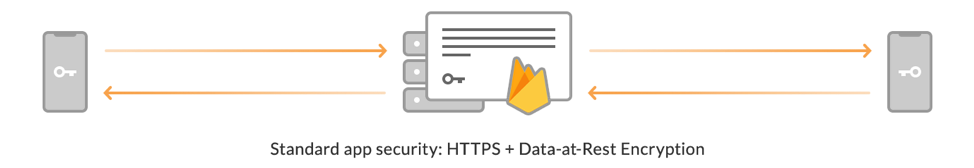
\includegraphics[width=15cm]{Backend_Implementierung/images/firebase_without_p2p_encryption.png}
		\caption{}
		\label{fig:firebase_without_encryption}
	\end{subfigure}\\
	\begin{subfigure}{\textwidth}
		\centering
		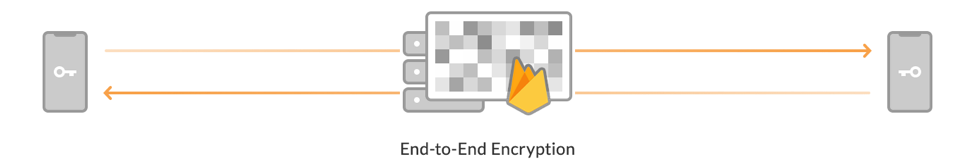
\includegraphics[width=15cm]{Backend_Implementierung/images/firebase_with_p2p_encryption.png}
		\caption{}
		\label{fig:firebase_with_encryption}
	\end{subfigure}
	\caption[]{ Firebase (a) ohne / (b) mit Ende-zu-Ende Verschlüsselung \protect \footnotemark}
\end{figure}
\footnotetext{Quelle: \url{https://virgilsecurity.com/blog/e3kit-for-firebase}, letzter Zugriff: 10. Mai 2021}



% Neue Section, neue Seite
\clearpage
\section{Implementierung der mobilen Anwendung}
Die Software für die mobile Anwendung wird ebenfalls in Komponenten/Module aufgeteilt. Abbildung \ref{fig:AppArchitektur} stellt die vereinfachte Architektur dar. Die Service-Komponenten dienen als Kommunikationsschnittstelle zum Senden für HTTPS-Anfragen. Die  Manager-Komponenten nutzen diese Schnittstellen und führen im Hintergrund des Programms verschiedene Tätigkeiten aus. Das User Interface (UI) stellt die Benutzeroberflächen dar und kann auf die Funktionen und Daten der Manager zurückgreifen.
\begin{figure}[tbt]
\centering
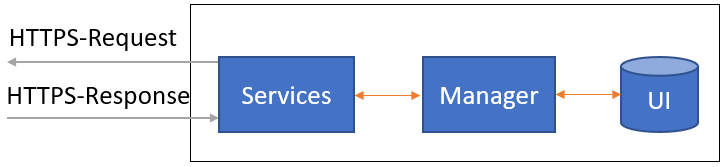
\includegraphics[width=10cm]{images/AppBackend.PNG}
\caption{Webserver Architektur}
\label{fig:AppArchitektur}
\end{figure}


%TODO Ersten 3 Kapitel sind Backend, weitere sind Frontend
\subsection{Klassenmodelle}		
Nachfolgend werden die Klassenmodelle innerhalb der mobilen Anwendung dargestellt.\\
\noindent
Die Filmdaten, die der Nutzer für das Swipen auf der Oberfläche erhält, werden aus dem Webserver bezogen. Der Informationsgehalt eines Films beschränkt sich dabei auf den eindeutigen Identifikator (ID) und den Titel des Films.
Im weiteren Schritt werden anhand der Film-ID's die weiteren benötigten Informationen aus dem TMDB-Server angefragt. \\

\noindent
\textbf{Movie Modell:}
Zum Konvertieren des JSON-Objekts aus dem Webserver und zum Speichern der Daten in die Umgebung der mobilen Anwendung wird die Klasse 'Movie' erstellt\footnote{Zum Konvertieren von JSON Objekten in Dart-Code wurde die Online-Konvertierung \url{https://app.quicktype.io/} genutzt.}. 


\begin{lstlisting}[caption=Movie Modell - JSON Konvertierung, label=lst:moviemodel]
Movie movieFromJson(String str) => Movie.fromJson(json.decode(str));
String movieToJson(Movie data) => json.encode(data.toJson());

class Movie {
  Movie({
    this.original_title,
    this.id
  });

  String original_title;
  String id;

  factory Movie.fromJson(Map<String, dynamic> json) => Movie(
    original\_title: json["original_title"],
    id: json["id"],
  );

  Map<String, dynamic> toJson() => {
    "original\_title": original_title,
    "id": id,
  };
}
\end{lstlisting}

\noindent
\textbf{TMDB-Movie Modell:}
Die Klasse 'TMDBMovie' ist eine Zusammenstellung mehrerer Daten. Sie enthält jeweils ein Objekt der folgenden aufgelisteten Klassen:

\begin{itemize}
\item \textbf{TmdbMovieDetails:} Enthält filmbezogene Informationen wie Titel, Posterpfad, Rating..
\item \textbf{TmdbMovieCredits:} Enthält Informationen zu den mitwirkenden Personen wie Schauspieler und Regisseure.
\item \textbf{TmdbMovieProvider:} Enthält Informationen bezüglich anbietenden Streaming-Providern.
\item \textbf{TmdbMovieTranslations:} Enthält Informationen zu Sprachen zum Film.
\end{itemize}

\noindent
\textbf{Match Modell:}
Nutzer werden ihre Matches vom Webserver abfragen. Hierbei erhalten erhalten sie zwei Listen 'supermatches' und 'normalmatches' sowie die Informationen 'newChanges', die Auskunft darüber gibt, ob es seit der letzten Anfrage zu Änderungen kam. Die Listen sind jeweils mit den entsprechenden Matchinformationen gefüllt. Der Informationsgehalt begrenzt sich auf die 'uid' der Nutzer und die 'id' des Films/der Filme, über das beide Nutzer gematcht sind. Für die Konvertierung und Speicherung dieser Informationen wurde die Klasse 'PartInformationMatches' erstellt. \\
Für die Darstellung eines Matches werden jedoch weitere Informationen wie der Titel oder der Posterpfad des Filmes und dem Namen des gematchten Nutzers. Die Klasse 'FullInformationMatches' enthält Eigenschaft für die Speicherung dieser zusätzlichen Daten.

\subsection{Kommunikationschnittstellen}
Die Kommunikationsanfragen an den Webserver und den Filmdatenbankserver TMDB werden auf einzelne Service-Komponenten aufgeteilt, die jeweils das von Dart zur Verfügung gestellte HTTP-Package \footnote{Offizielle Homepage : \url{https://pub.dev/packages/http}} implementieren.\\
Da der Webserver in der Entwicklungsphase einen selbstsigniertes Sicherheitszertifikat hat, wird für die HTTPS-Kommunikation die 'badCertificateCallback'-Funktion des 'HttpClient'-Objekts im HTTP-Package umgeschrieben. Es sei zu erwähnen, dass dieser Workaround nur in der Entwicklung genutzt werden soll. 

\begin{lstlisting}[caption=Bad Certificate - Workaround, label=lst:badcertificateworkaround]
class DevHttpOverrides extends HttpOverrides {
  @override
  HttpClient createHttpClient(SecurityContext context) {
    return super.createHttpClient(context)
      ..badCertificateCallback =
          (X509Certificate cert, String host, int port) => true;
  }
}
\end{lstlisting}

\noindent
Die Implementierung soll im Weiteren anhand der 'MoviesRequest'-Funktion des Movie-Services dargestellt werden. Die Funktionen der User-, Match- und Swipe-Services sind im ähnlichen Stil gehandhabt. \\

\noindent
\textbf{Movie Service:}
Der Movie-Service bietet die Funktion 'MoviesRequest', welche einen Post-Anfrage über HTTPS an die Serveradresse (URL) und dem dazugehörigen relativen Pfad '/movies/request' sendet. Dafür wird zunächst ein Objekt 'data' erstellt, das mit den als Parameter übergebenen Daten gefüllt wird, die für die serverseitige Abhandlung der Anfrage benötigt werden. Über die 'post'-Funktion wird die Anfrage an die übergebene URL gesendet. Dem Header muss bei Übergabe von JSON-Daten der Eigenschaft 'Content-Type' der Wert 'application/json' hinzugefügt werden. Dem Body wird das aus 'data' in JSON codierte Objekt übergeben. Nach Ankunft der Antwort wird über den Statuscode geprüft, ob die Anfrage problemfrei ausgeführt werden konnte. Letztlich wird eine Liste von Movie-Objekten, die aus den im Body der Antwort befindlichen JSON-Daten konvertiert wurden, erstellt und zurückgegeben.

\begin{lstlisting}[caption=Movie Service - MoviesRequest, label=lst:MoviesRequest]
static Uri _url_Request = Uri.parse('https://' + URL + ':3001/movies/request');

static Future<List<Movie>> MoviesRequest(final List<String> internMovieList,
final int movieAmount,final bool includeSwiped) async {
 var _responseBody;
 String _uidtoken = await UserManager().getUserToken();

 //Body mit JSON fuellen
 Map data = { 'alreadyRequestedMovieIDs': internMovieList,
              'includeSwiped': includeSwiped,
              'amount': movieAmount,
              'uidtoken': _uidtoken };
              
 var body = json.encode(data);
 // Daten senden
 try { var response = await http.post(_url_Request,
       headers: {"Content-Type": "application/json"},
       body: body).timeout(Duration(seconds: 10),onTimeout: (){
                                          throw Exception(); });
      
       _responseBody = response.body;
       if(response.statusCode != 200)
       { throw(_responseBody);}
 }
 catch(Exception){return null;}

 List collection = json.decode(_responseBody);
 return collection.map((json) => Movie.fromJson(json)).toList();
}
\end{lstlisting}



\noindent
\textbf{User Service:} Dieser Service enthält die User-bezogenen Funktionen 'CreateUser' und 'ChangeUser', die entsprechende Anfragen an den Webserver schicken.\\

\noindent
\textbf{Match Service:} Dieser Service enthält die Match-bezogenen Funktionen 'MatchesRequest', 'DeleteSupermatch' und 'DeleteNormalmatch'.
Ausserdem wird für die Entwicklungsphase die 'Trigger'-Funktion angeboten.
Die Funktionen des Match-Services senden die dem Namen entsprechenden Anfragen an den Webserver.\\

\noindent
\textbf{Swipe Service:}
Dieser Service enthält lediglich die Funktion 'CreateSwipe', die die entsprechende Anfrage an den Webserver schickt.\\

\noindent
\textbf{TMDB Service:}
Der TMDB-Server bietet eine Programmierschnittstelle, auch Application Programming Interface (API) genannt, zum Abfragen von Daten\footnote{Offizielle Seite der API: \url{https://www.themoviedb.org/documentation/api}}. 
Die nachfolgend aufgelisteten Funktionen fragen entsprechend dem benötigten Informationsgehalt unterschiedliche URL'S an. 
Dabei wird jeweils der URL eine ID eines Filmes mitgegeben. Die in der Antwort zurückgesendeten Daten beziehen sich auf die übergebene Film-ID. 
Dem Namen der Funktion entsprechend wird ein Objekt der Klasse 'TMDBMovieDetails', 'TMDBMovieCredits', 'TMDBMovieProviders' oder 'TMDBMovieTranslations' zurückgegeben.

\begin{itemize}
\item Request Details
\item Request Credits
\item Request Providers
\item Request Translations
\end{itemize}
	
\subsection{Manager}	
Die Manager-Klassen regeln die Backend-Funktionalitäten, die vom Nutzer nicht direkt ersichtlich sind. \\

\noindent
\textbf{Swipe Manager: }
Der Swipe Manager verwaltet sowohl die Filme, die in der Benutzeroberfläche geswipet werden können, als auch getätigten Swipes des Nutzers. Er agiert im Hintergrund des Programms. Dabei pflegt er eine Liste von Filmen, dessen Anzahl er periodisch überprüft. Wird eine bestimmte Mindestanzahl erreicht, frägt er den Webserver nach neuen Filmen, die der Nutzer weder bereits geswipet, noch geladen hat. 
Anschließend werden für jeden erhaltenen Film sämtliche Funktion des TMDB-Services mit der jeweiligen Film-ID aufgerufen und die zurückerhaltenen Objekte als TMDBMovie-Objekte in einer weiteren Liste gespeichert. Die daraus generierte Liste kann nun an das User-Interface zum Swipen übergeben werden.
Ein Swipen hat zur Folge, dass der davon betroffene Film aus der Liste entfernt wird und der Webserver die Informationen über diesen Swipe-Vorgang erhält.
Für die entsprechenden Anfragen an den Webserver nutzt der Swipe Manager den Movie- und den Swipe-Service. \\

\noindent
\textbf{User Manager:}
Dieser Manager verwaltet userbezogene Daten der mobilen Anwendung. Sie ist ausserdem für die Verwaltung des Firebase-Tokens zuständig und frägt bei abgelaufenem oder invaliden Token einen neuen ab. \\

\noindent
\textbf{Match Manager:}
Der Match Manager delegiert die Match-bezogenen Anfragen an den Match-Service weiter. Ausserdem verwaltet er bereits abgefragte Matches. Innerhalb der 'RequestMatches'-Funktion ruft er neben der Delegierung an den Match-Service weitere Funktionen aus. Zum einen werden anhand der mitüberlieferten Film'IDs Anfragen über den TMDB-Service an den TMDB-Server gesendet, mit dem Zweck, den zugehörigen Filmtitel und Posterpfad abzufragen. Zum Anderen wird eine Anfrage an Firebase zum Erhalt der 'uid' des gematchen Nutzers geschickt.
Zur Verhinderung von redundanten Abfragen der Zusatzinformationen zwischen aufeinanderfolgenden Match-Abfragen wird innerhalb der Funktion 'requestMovies' zunächst auf die erhaltene 'newChanges'-Eigenschaft geprüft. Nur wenn dessen Wert dem booleschen Wert true gleicht, werden die Anfragen an TMDB und Firebase ausgeführt. Andernfalls wird die gleiche Liste, die aus vorherigen Match-Anfrageresultaten im Match-Manager zwischengespeichert wurden, zurückgegeben. \\
%-------------------------------------
%\subsection{Swipe/Aussuchen/Voting}		
%\subsection{Matches/Chat}		
%\subsection{Film-/Serienvorschläge}
%\subsection{Gespeicherte Filme/Filmliste}		
%\subsection{Barrierefreiheit}
%\label{sec:barrierefreiheit}
%
Barrierefreiheit im Allgemeinen bedeutet, dass ein Gegenstand, eine Einrichtung oder Informationsquelle für Menschen mit Behinderung ohne Unzulänglichkeiten nutzbar, zugänglich oder auffindbar ist (\cite{behindertengleichstellungsgesetz}, §4). In der Softwareentwicklung versteht man darunter Applikationen für Menschen mit Einschränkungen zugänglich und bedienbar zu machen. Bezogen auf die Entwicklung von  mobilen Apps gilt es dabei den akustischen, optischen oder motorischen Einschränkungen der Benutzer entgegenzuwirken. \\

%\subsubsection{Barrierefreiheit in mobilen Anwendungen}
%Mit der Verbreitung von Smartphones ist die Benutzung mobiler Apps stark angestiegen und mittlerweile in nahezu jedem Haushalt aufzufinden. Obwohl etwa 9,5\% aller in Deutschland lebenden Menschen einen Schwerbehindertenausweis besitzen (Stand 24. Juni 2020)\cite{schwerbehindertenausweis} was etwa 7,9 Millionen Menschen entspricht, ist die Implementierung von barrierefreier Bedienung nicht selbstverständlich. Gerade Programmierern/innen aus dem privaten Sektor sind diese Funktionen oft nicht bekannt, es besteht kein Interesse oder sie werden schlichtweg vergessen. Software, die für öffentliche Einrichtungen entwickelt wird, ist durch das Behindertengleichstellungsgesetz von 2002 dazu verpflichtet ihr Softwareangebot bis spätestens dem 23. Juni 2021 barrierefrei zu gestalten (\cite{behindertengleichstellungsgesetz}, §12a Abs.1). Hierzu zählen sämtliche Webseiten sowie mobile Anwendungen. \\

%\subsubsection{Barrierefreiheit in Filmen und Serien}
%Auch die Zugänglichkeit von Filmen und Serien für Menschen mit eingeschränkter Wahrnehmung wurde in den letzten Jahren stark verbessert. 
Hierbei lässt sich zwischen optischer und akustischer Einschränkung differenzieren. Für hörgeschädigte Personen werden bereits seit mehreren Jahrzehnten Untertitel eingesetzt. Was früher für vereinzelte Filme durch eine Funktion des Teletextes erreicht wurde, wird heutzutage durch eine integrierte Funktion des Videoplayers verwirklicht. Immer mehr Videos werden mit Untertiteln veröffentlicht. Manche Anbieter wie beispielsweise die Internetplattform YouTube bieten durch Spracherkennung automatisch generierte Untertitel an, was eine flächendeckende Untertitelung ermöglicht.\\
Auch für Menschen mit eingeschränktem Sehvermögen werden Filme und Serien mithilfe von Audiodeskriptionen vermehrt zugänglich gemacht. Hierbei wird die bereits vorhandene Tonspur mit Bildbeschreibungen und Kommentaren versehen. Was bis vor wenigen Jahren noch etwas Besonderes war und nur für ausgewählte Filme bestimmt war, ist heutzutage Standard. Größere Video-On-Demand-Plattformen wie Netflix oder Amazon Prime bieten diese Möglichkeit bei nahezu allen Eigenproduktionen an. Zusätzlich werden bestehende Filme neu mit Audiodeskriptionen versehen.\\


\noindent Hieraus lässt sich leicht erkennen, dass Filme und Serien heutzutage auch von Menschen mit Einschränkungen genutzt werden. Was auf den ersten Blick vielleicht nicht bedacht wird oder als  unwichtig abgestempelt wird, kann einen nicht unerheblichen Vergrößerungsfaktor für den Kundenstamm bewirken. Für die Entwicklung einer mobilen App, bei der Filme und Serien bewertet werden, spielt also die Barrierefreiheit eine wichtige Rolle und darf auf keinen Fall vernachlässigt werden. 

%\subsubsection{Barrierefreiheit bei StreamSwipe}
%\label{sec:bf-streamswipe}
%
Bei der Entwicklung von StreamSwipe werden mehrere mögliche Einschränkungen der Nutzer betrachtet und entsprechend reagiert. Ziel ist es, dass sowohl der Kunde sowie der Anbieter maximal davon profitieren. Hierfür soll die App für ein möglichst großes Publikum zugänglich gemacht werden, jedoch auch sogenanntes Over-Engineering vermieden werden, da zu viele Funktionen eine App unübersichtlich, teuer und langsamer werden lassen.\\

\noindent
Allgemein wird Leserlichkeit durch große Schriftgrößen, hohe Farbkontraste, große Schaltflächen oder universelles Design erreicht. Alleine in Deutschland tragen 44,5 Millionen Menschen regelmäßig eine Brille oder Kontaktlinsen und benötigen somit Sehhilfen \cite{sehhilfen}. Unterstützung auf Seiten der App kann hierfür durch vergrößerbaren Text geschehen. Da aber davon ausgegangen werden kann, dass Personen, die sich auf Sehhilfen verlassen, bereits eine Brille oder Kontaktlinsen besitzen, wird die Textgröße vorerst nicht variabel gehalten. Außerdem gibt es bei Android- und Apple-Smartphones bereits eingebaute Vergrößerungsfeatures, die Bildausschnitte vergrößert darstellen können. Aus diesem Grund wird in diesem Projekt kein Fokus auf dieses Feature gelegt. \\
Farbblindheit kann jedoch in vielen Formen auftreten. Um der bekannten Farbfehlsicht entgegenzuwirken, werden Farben aus Problembereichen wie Rot und Grün nicht nebeneinander benutzt. Allgemein wird ein schlichtes Design gewählt und Farben nur zu Akzentuierung und als Stilmittel benutzt (vgl. Abbildungen \ref{fig:BF-Beispiele}), statt als Informationsträger.  Geringe Sehschärfe durch Achromatopsie kann wie weiter oben beschrieben umgangen werden.\\


\begin{figure}[tbt]
	\begin{subfigure}{0.5\textwidth}
	\centering
	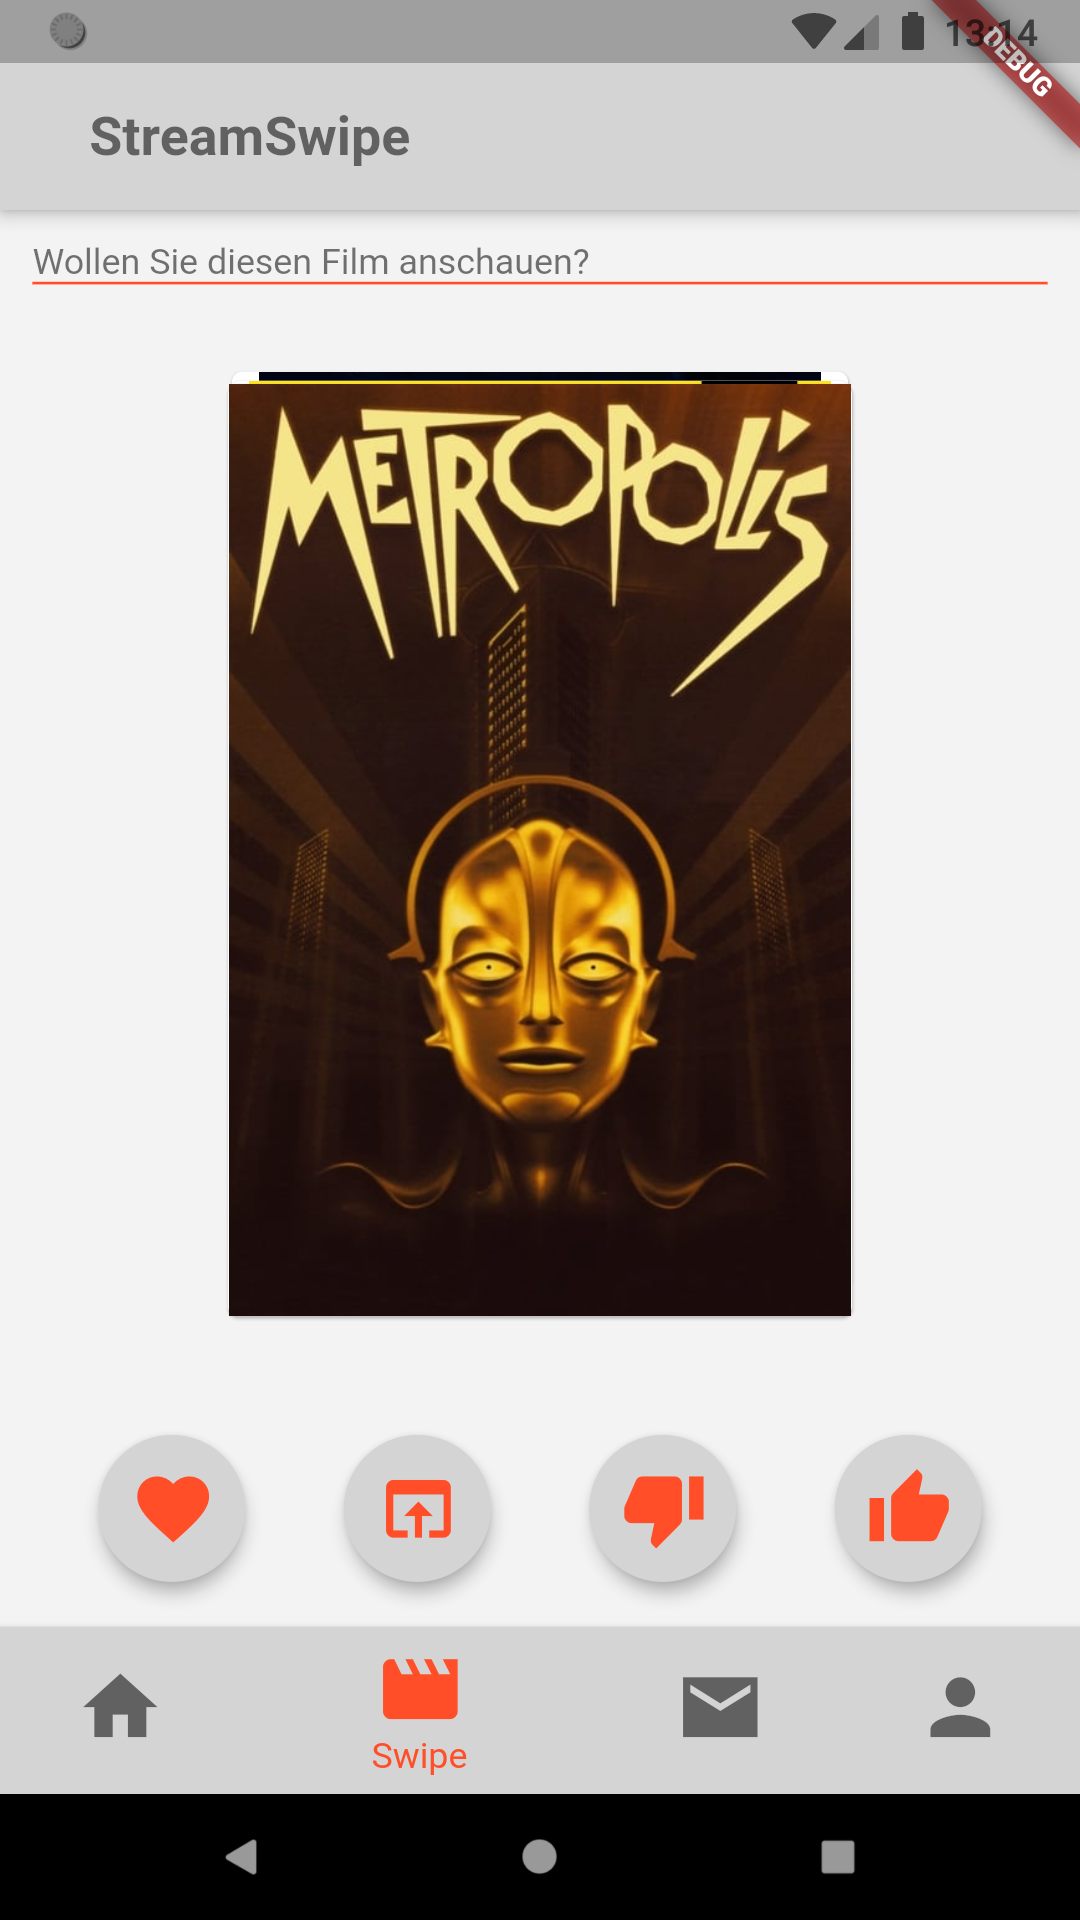
\includegraphics[scale=0.15]{Barrierefreiheit/images/bsp-swipe.png}
	\caption{}
	\label{fig:bf-beispiel_a}
	\end{subfigure}
	\begin{subfigure}{0.5\textwidth}
	\centering
	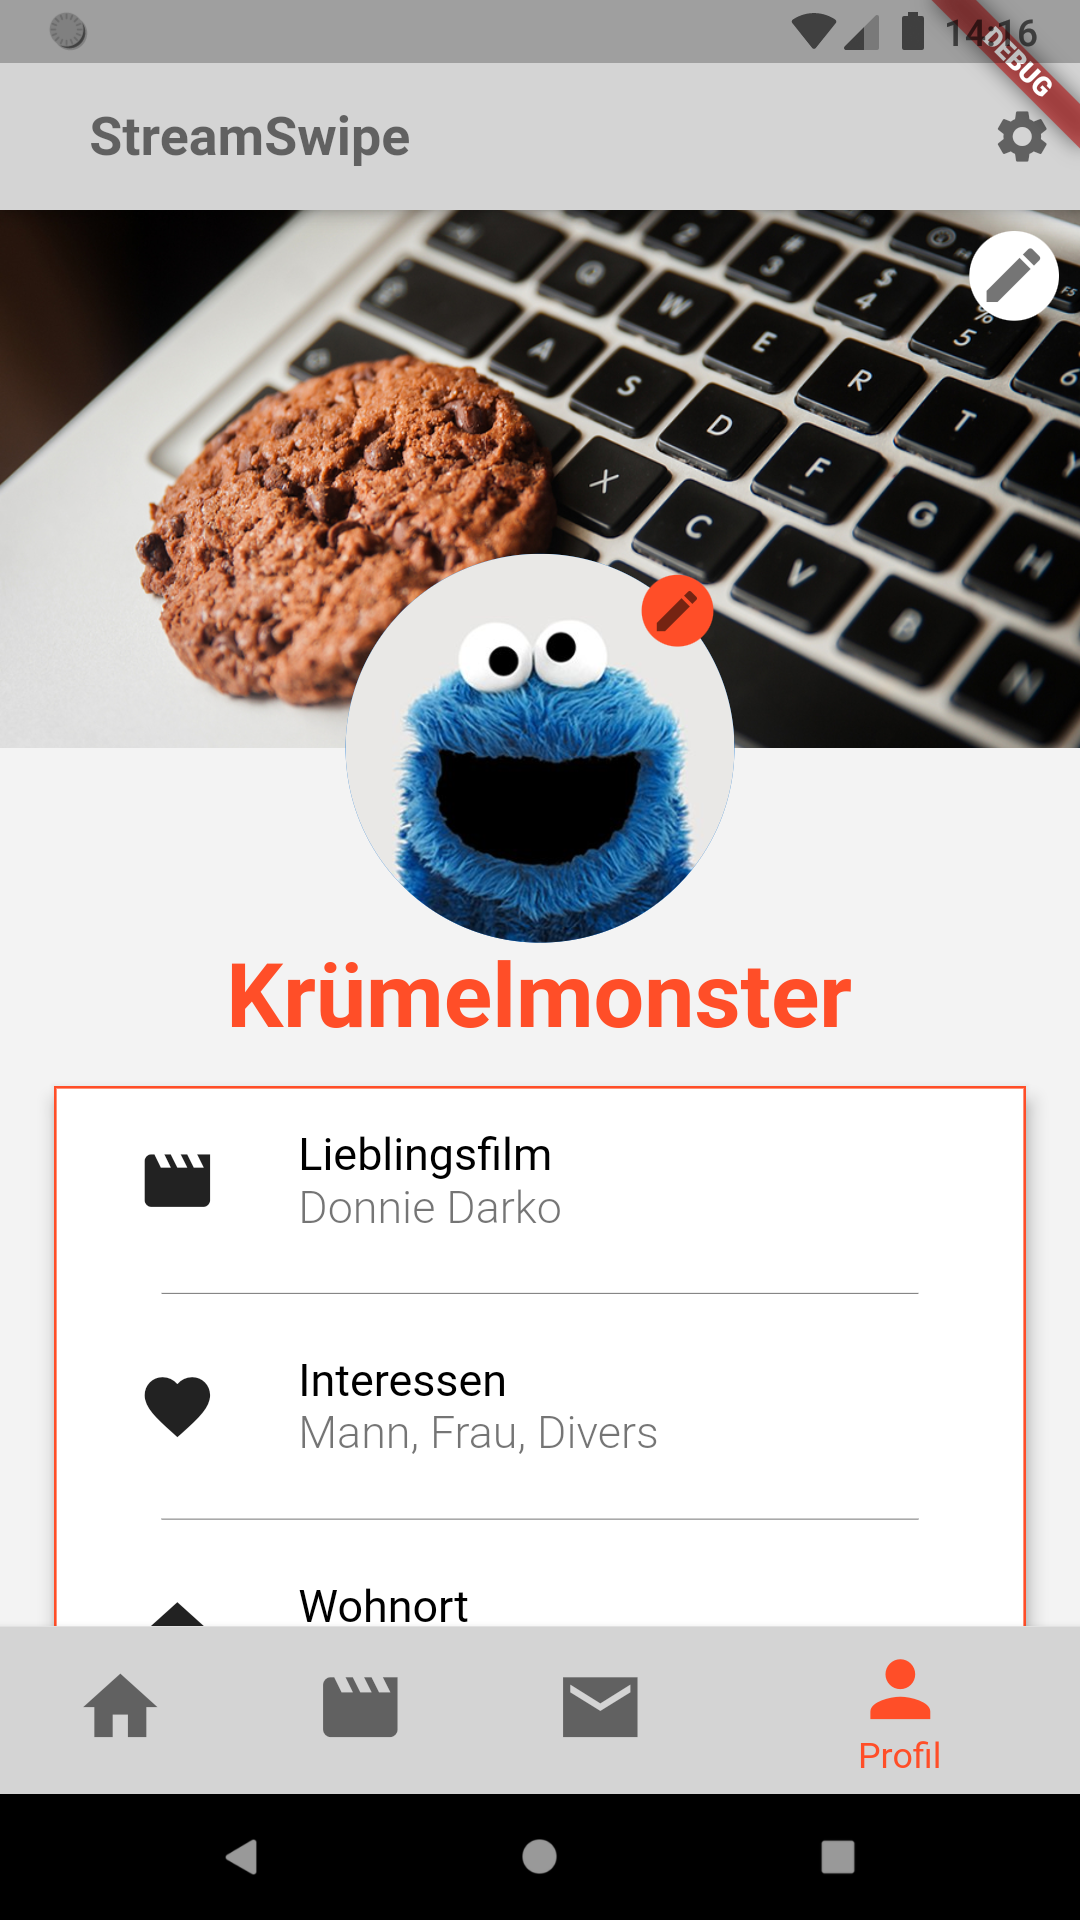
\includegraphics[scale=0.15]{Barrierefreiheit/images/bsp-profil.png}
	\caption{}
	\label{fig:bf-beispiel_b}
	\end{subfigure}
\caption[Screenshots als Beispiele für Barrierefreiheit]{Screenshots aus der App StreamSwipe als Beispiele zu (a) schlichtem Design, bei dem farbige Akzente nicht der Informationenübertragung dienen um die Zugänglichkeit für farbblinde Menschen zu verbessern und für einen Icon in (b), welcher sonst durch sehgeschädigte Menschen nicht wahrnehmbar ist, wird exemplarisch eine Semantik implementiert.}
\label{fig:BF-Beispiele}
\end{figure}


\noindent
Ist die Sehkraft noch weiter eingeschränkt oder gar nicht mehr vorhanden, werden Semantiken eingesetzt. Hierbei erhält jedes Element auf dem Bildschirm eine Beschreibung, die vorgelesen werden kann. Bei Zahlen und Texten werden diese vorgelesen, sofern keine weitere Information hinterlegt ist. Besonders hilfreich ist dies jedoch bei Abbildungen. Ausgeführt wird das Auslesen von einem Screenreader. Mobile Geräte haben diese Funktion bereits standardmäßig eingebaut (VoiceOver bei Apple und TalkBack bei Android) und wandeln die Semantiken mittels Sprachsynthese in akustische Signale um. Bei Desktopanwendungen wie z.B. JAWS für Windows können diese Informationen zusätzlich auch durch eine Braillezeile wiedergegeben werden.\\
Bei Flutter ist das Hinzufügen von Semantiken bereits eingebaut. Hierfür kann ein String dem jeweiligen Bereich zugeordnet werden. In Beispiel \ref{lst:semantics} ist hierfür der Code des Buttons, der zu den Einstellungen führt. In Abbildung \ref{fig:bf-beispiel_b} ist dieser Button ganz rechts oben im Eck zu sehen.\\
Die Funktion \texttt{GestureDetector()} erkennt Interaktionen mit dem Touchscreen, wobei hier nur auf Antippen reagieren soll, deshalb die Funktion \texttt{onTap:()$\{\}$}, die auf den Einstellungsbildschirm leitet. Diese Implementierung ist hier aber nicht von Relevanz und wird übersprungen. In dem \texttt{GestureDetector()} ist ein Icon eingebettet, von der Form \textit{Settings}, was einem Zahnrad entspricht. Dieses Icon erhält eine Farbe und anschließend eine Semantik aus allem was in den Anführungszeichen steht. Ein Screenreader kann AE erkennen und ihn als den Umlaut Ä aussprechen. \\
So wird im kompletten Programm für jedes relevante Element vorgegangen. Teilweise  müssen den Semantiken Variablen übergeben werden, da sich die vorzulesende Information ändert wie beispielsweise bei den Filmtiteln.
    
\begin{lstlisting}[caption=Codeausschnitt in Dart von einem Button mit Semantiken.,label=lst:semantics]
GestureDetector(
  onTap: () {
     ...
  },
  child: Icon(
    Icons.settings,
    color: Provider.of(context).colors.textSmall,
    semanticLabel: "Einstellungen. Zum Auswaehlen doppeltippen.",
  )
),
\end{lstlisting}

\noindent
Bei einer sauberen Implementierung wird auf diese Weise vorgegangen und eine bereits vorhandene Funktion verwendet. Dies vereinfacht nicht nur die Leserlichkeit des Codes, sondern bietet auch die höchste Modularität, da hierbei normalerweise standardisierte Schnittstellen für Betriebssysteme oder andere Anwendungen verwendet werden. In diesem Fall  müssen die Screenreader von Android und Apple damit arbeiten können.\\

\noindent 
Um für Personen mit eingeschränktem Hörvermögen oder vollständiger Gehörlosigkeit die App zugänglich zu machen, wird auf akustisches Feedback als notwendige Infor"-mations"-über"-tragung verzichtet. Innerhalb der App werden keine Geräusche erzeugt, außer der oben beschriebenen Funktion der Semantiken. Beim Erhalten einer neuen Nachricht oder eines neuen Matches kann weiterhin optional eine akustische Benachrichtigung erhalten werden. Hierbei wird die betriebssystemeigene Funktion übernommen, sodass in der App keine neuen Einstellungen vorgenommen werden müssen.\\

\noindent
Auch feinmotorische Einschränkungen werden versucht zu umgehen. Die Navigation und die Filmbewertung in StreamSwipe können durch großflächige Wischbewegungen ausgeführt werden. Wo diese Lösung nicht möglich ist, werden verhältnismäßig große Buttons eingesetzt. Lediglich beim Registrieren und Einloggen werden feine Bewegungen erfordert. Hierbei öffnet sich allerdings die als Standard eingestellte digitale Tastatur, die in vielen Fällen eine Spracheingabe besitzt, sodass die sehr kleinen Tasten nicht benutzt werden müssen.\\

%TODO Diesen Satz evtl. ganz ans Ende ins Fazit
\noindent
Sollte sich in Zukunft jedoch Kritik in Form von negativen Nutzerbewertungen herauskristallisieren, kann eines der noch nicht implementierten Features über ein Update nachgerüstet werden.
%\clearpage

% Neue Section, neue Seite
\clearpage
\section{Benutzeroberflächen der mobilen Anwendung}
\label{sec:UI-allgemein}
Die Benutzeroberfläche einer Software muss im Grunde genommen nur einen Informationsfluss in zwei Richtungen erzeugen. Die eine Richtung liefert Informationen an den User und über die andere kann der User Informationen an das System weitergeben. Um auf dem heutigen Markt Fuß fassen zu können, sollte eine Oberfläche jedoch wesentlich mehr Aspekte erfüllen. 



\subsection{Aspekte von Benutzeroberflächen}
\label{sec:UI-Aspekte}
Die Vielschichtigkeit einer Benutzeroberfläche kann ausschlaggebend für den Erfolg einer Applikation sein, abhängig davon welche Erfahrungen der User mit der Oberfläche macht und welche Eindrücke sie hinterlässt. Hieraus resultiert wie lange ein User auf der App bleibt und wie oft er zurück kommt. Neben der Nutzungszeit erhöht eine positive User Experience die Weiterempfehlungsrate.\\
Bei erfolgreicher Software besteht ein großer Teil der Entwicklung in der Planung der Oberfläche, da die User Experience nicht zu umgehen ist. Auf die eine oder andere Art erlebt der User immer eine Erfahrung. Neben den offensichtlichen Aus- und Eingabefunktionen werden beispielsweise folgende Kriterien  betrachtet:\\

\noindent
\hangindent1cm
\textbf{Simpel:} Ausgegebene Information kann zum Beispiel durch Icons, Farben oder Symbole vereinfacht werden. Eine Oberfläche sollte weder überladen sein, noch sollten alle Ein- und Ausgaben auf verschiedenen Screens verteilt sein. Bei der Entwicklung wird eine gesunde Mischung aus maximaler Funktionalität und einfacher, übersichtlicher Darstellung angestrebt.\\

\noindent
\hangindent1cm
\textbf{Einheitlich:} Die Bedienung und das Lesen von Applikationen kann erheblich vereinfacht werden wenn einheitliche Bedien- oder Ausgabeelemente verwendet werden. Nicht nur innerhalb einer App ist es sinnvoll konsistente Elemente in der Oberfläche zu verwenden, auch Funktionen von anderen Apps können die Bedienung vereinfachen. Bekannte Funktionen bei Smartphone-Applikationen sind zum Beispiel die Vergrößerung mit zwei Fingern oder das \glqq Daumen nach oben\grqq -Symbol als positive Rückmeldung. Durch das  Einbauen solcher Features wird eine App intuitiv und ohne Einführung bedienbar.\\

\noindent
\hangindent1cm
\textbf{Benutzergesteuert:} Alle ausgeführten Aktionen sollten vom Benutzer ausgehen. Ein gutes Interface unterstützt den User lediglich bei seiner Bedienung, schränkt ihn aber nicht ein. Mit der heutigen Technologie ist die Verführung groß viele Funktionen automatisch ablaufen zu lassen. Was eigentlich der Sinn einer Applikation ist, kann jedoch auch negative Folgen haben. Zu viel Automatisierung verursacht das Gefühl von Kontrollverlust und Unsicherheit, was sich negativ auf das Vertrauen und somit auf die Benutzungszeit von dem User auswirkt. \\

\noindent
\hangindent1cm
\textbf{Klarheit:} Eine mobile App muss ohne Anleitung bedienbar sein. Sobald Unklarheiten beim User entstehen und Funktionen oder Ausgaben nicht erkannt werden können, verliert die Anwendung auf dem freien Markt. \\
Der User sollte zu jeder Zeit wissen welche Optionen ihm zur Verfügung stehen und welche Folgen seine Aktionen haben. Besonders wichtig ist das Feedback infolge einer Aktion. Auch wenn diese Aspekte offensichtlich erscheinen, können sie bei der Entwicklung einer App leicht übersehen werden. Verwendet werden einfache und für den User bekannte Funktionen, wie die Beschriftung aller Buttons oder das haptische, akustische oder optische Feedback beim drücken einem dieser Buttons.\\

\noindent
\hangindent1cm
\textbf{Benutzerfreundlich/Barrierefreiheit:} Die Bedienung der App sollte für Menschen mit Einschränkungen im vollen Umfang möglich sein. In Abschnitt \ref{sec:barrierefreiheit} wird auf dieses Thema tiefer eingegangen. Aber auch Benutzer ohne Einschränkungen erwarten eine einfache und übersichtliche Bedienung, die auch beispielsweise  Eingabefehler mit mehreren Versuchen verzeiht.\\

\noindent
\hangindent1cm
\textbf{Ästhetik:} Das Design spielt bei dieser Betrachtung gleich mehrere wichtige Rollen. Es sollte eine angenehme Arbeitsumgebung für den User erstellen, Ein- und Ausgaben verdeutlichen und gleichzeitig mithilfe eines eigenen Stils ein einzigartiges Image für die App schaffen (sogenanntes Branding) um deren Individualität und Wiedererkennungswert zu steigern. Das Design erschafft ein Erlebnis während der Benutzung und weckt Gefühle im User. \\

\noindent
Gerade weil viele dieser Aspekte unterbewusst wirken, ist eine ausgiebige Betrachtung unumgänglich.\\
Eine Schwierigkeit, die sich bei der Entwicklung ergibt sind die zwei unterschiedlichen Ziele. Einerseits sollten bestehende Design- und Bedienelemente  übernommen werden um die Bedienung intuitiv und übersichtlich zu gestalten, andererseits aber auch neue Ideen und Innovationen eingebracht werden, um sich von anderen Apps abzuheben und bleibenden Wiedererkennungswert aufzubauen.

\subsection{Barrierefreiheit}
\label{sec:barrierefreiheit}

Barrierefreiheit im Allgemeinen bedeutet, dass ein Gegenstand, eine Einrichtung oder Informationsquelle für Menschen mit Behinderung ohne Unzulänglichkeiten nutzbar, zugänglich oder auffindbar ist (\cite{behindertengleichstellungsgesetz}, §4). In der Softwareentwicklung versteht man darunter Applikationen für Menschen mit Einschränkungen zugänglich und bedienbar zu machen. Bezogen auf die Entwicklung von  mobilen Apps gilt es dabei den akustischen, optischen oder motorischen Einschränkungen der Benutzer entgegenzuwirken. \\

\subsubsection{Barrierefreiheit in mobilen Anwendungen}
Mit der Verbreitung von Smartphones ist die Benutzung mobiler Apps stark angestiegen und mittlerweile in nahezu jedem Haushalt aufzufinden. Obwohl etwa 9,5\% aller in Deutschland lebenden Menschen einen Schwerbehindertenausweis besitzen (Stand 24. Juni 2020)\cite{schwerbehindertenausweis} was etwa 7,9 Millionen Menschen entspricht, ist die Implementierung von barrierefreier Bedienung nicht selbstverständlich. Gerade Programmierern/innen aus dem privaten Sektor sind diese Funktionen oft nicht bekannt, es besteht kein Interesse oder sie werden schlichtweg vergessen. Software, die für öffentliche Einrichtungen entwickelt wird, ist durch das Behindertengleichstellungsgesetz von 2002 dazu verpflichtet ihr Softwareangebot bis spätestens dem 23. Juni 2021 barrierefrei zu gestalten (\cite{behindertengleichstellungsgesetz}, §12a Abs.1). Hierzu zählen sämtliche Webseiten sowie mobile Anwendungen. \\

\subsubsection{Barrierefreiheit in Filmen und Serien}
Auch die Zugänglichkeit von Filmen und Serien für Menschen mit eingeschränkter Wahrnehmung wurde in den letzten Jahren stark verbessert. 
Hierbei lässt sich zwischen optischer und akustischer Einschränkung differenzieren. Für hörgeschädigte Personen werden bereits seit mehreren Jahrzehnten Untertitel eingesetzt. Was früher für vereinzelte Filme durch eine Funktion des Teletextes erreicht wurde, wird heutzutage durch eine integrierte Funktion des Videoplayers verwirklicht. Immer mehr Videos werden mit Untertiteln veröffentlicht. Manche Anbieter wie beispielsweise die Internetplattform YouTube bieten durch Spracherkennung automatisch generierte Untertitel an, was eine flächendeckende Untertitelung ermöglicht.\\
Auch für Menschen mit eingeschränktem Sehvermögen werden Filme und Serien mithilfe von Audiodeskriptionen vermehrt zugänglich gemacht. Hierbei wird die bereits vorhandene Tonspur mit Bildbeschreibungen und Kommentaren versehen. Was bis vor wenigen Jahren noch etwas Besonderes war und nur für ausgewählte Filme bestimmt war, ist heutzutage Standard. Größere Video-On-Demand-Plattformen wie Netflix oder Amazon Prime bieten diese Möglichkeit bei nahezu allen Eigenproduktionen an. Zusätzlich werden bestehende Filme neu mit Audiodeskriptionen versehen.\\


\noindent Hieraus lässt sich leicht erkennen, dass Filme und Serien heutzutage auch von Menschen mit Einschränkungen genutzt werden. Was auf den ersten Blick vielleicht nicht bedacht wird oder als  unwichtig abgestempelt wird, kann einen nicht unerheblichen Vergrößerungsfaktor für den Kundenstamm bewirken. Für die Entwicklung einer mobilen App, bei der Filme und Serien bewertet werden, spielt also die Barrierefreiheit eine wichtige Rolle und darf auf keinen Fall vernachlässigt werden. 

\subsubsection{Barrierefreiheit bei StreamSwipe}
\label{sec:bf-streamswipe}

Bei der Entwicklung von StreamSwipe werden mehrere mögliche Einschränkungen der Nutzer betrachtet und entsprechend reagiert. Ziel ist es, dass sowohl der Kunde sowie der Anbieter maximal davon profitieren. Hierfür soll die App für ein möglichst großes Publikum zugänglich gemacht werden, jedoch auch sogenanntes Over-Engineering vermieden werden, da zu viele Funktionen eine App unübersichtlich, teuer und langsamer werden lassen.\\

\noindent
Allgemein wird Leserlichkeit durch große Schriftgrößen, hohe Farbkontraste, große Schaltflächen oder universelles Design erreicht. Alleine in Deutschland tragen 44,5 Millionen Menschen regelmäßig eine Brille oder Kontaktlinsen und benötigen somit Sehhilfen \cite{sehhilfen}. Unterstützung auf Seiten der App kann hierfür durch vergrößerbaren Text geschehen. Da aber davon ausgegangen werden kann, dass Personen, die sich auf Sehhilfen verlassen, bereits eine Brille oder Kontaktlinsen besitzen, wird die Textgröße vorerst nicht variabel gehalten. Außerdem gibt es bei Android- und Apple-Smartphones bereits eingebaute Vergrößerungsfeatures, die Bildausschnitte vergrößert darstellen können. Aus diesem Grund wird in diesem Projekt kein Fokus auf dieses Feature gelegt. \\
Farbblindheit kann jedoch in vielen Formen auftreten. Um der bekannten Farbfehlsicht entgegenzuwirken, werden Farben aus Problembereichen wie Rot und Grün nicht nebeneinander benutzt. Allgemein wird ein schlichtes Design gewählt und Farben nur zu Akzentuierung und als Stilmittel benutzt (vgl. Abbildungen \ref{fig:BF-Beispiele}), statt als Informationsträger.  Geringe Sehschärfe durch Achromatopsie kann wie weiter oben beschrieben umgangen werden.\\


\begin{figure}[tbt]
	\begin{subfigure}{0.5\textwidth}
	\centering
	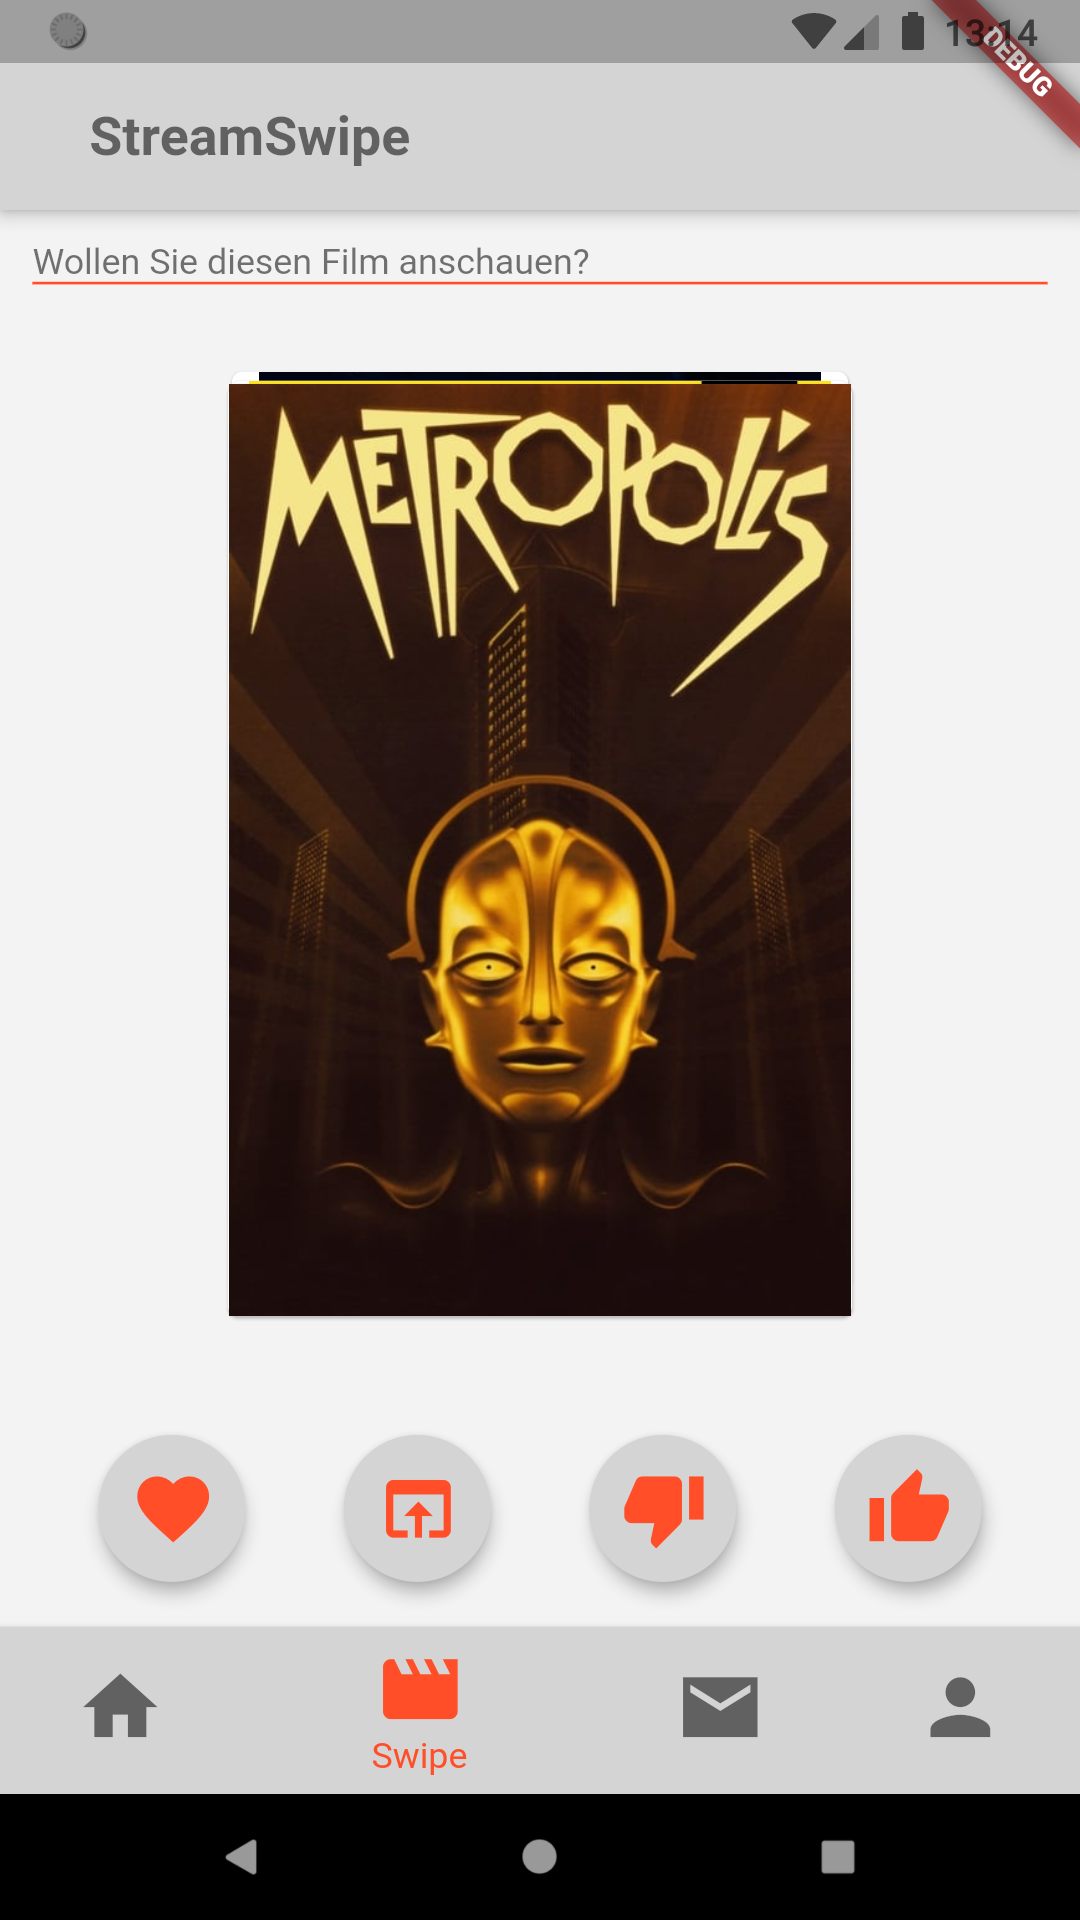
\includegraphics[scale=0.15]{Barrierefreiheit/images/bsp-swipe.png}
	\caption{}
	\label{fig:bf-beispiel_a}
	\end{subfigure}
	\begin{subfigure}{0.5\textwidth}
	\centering
	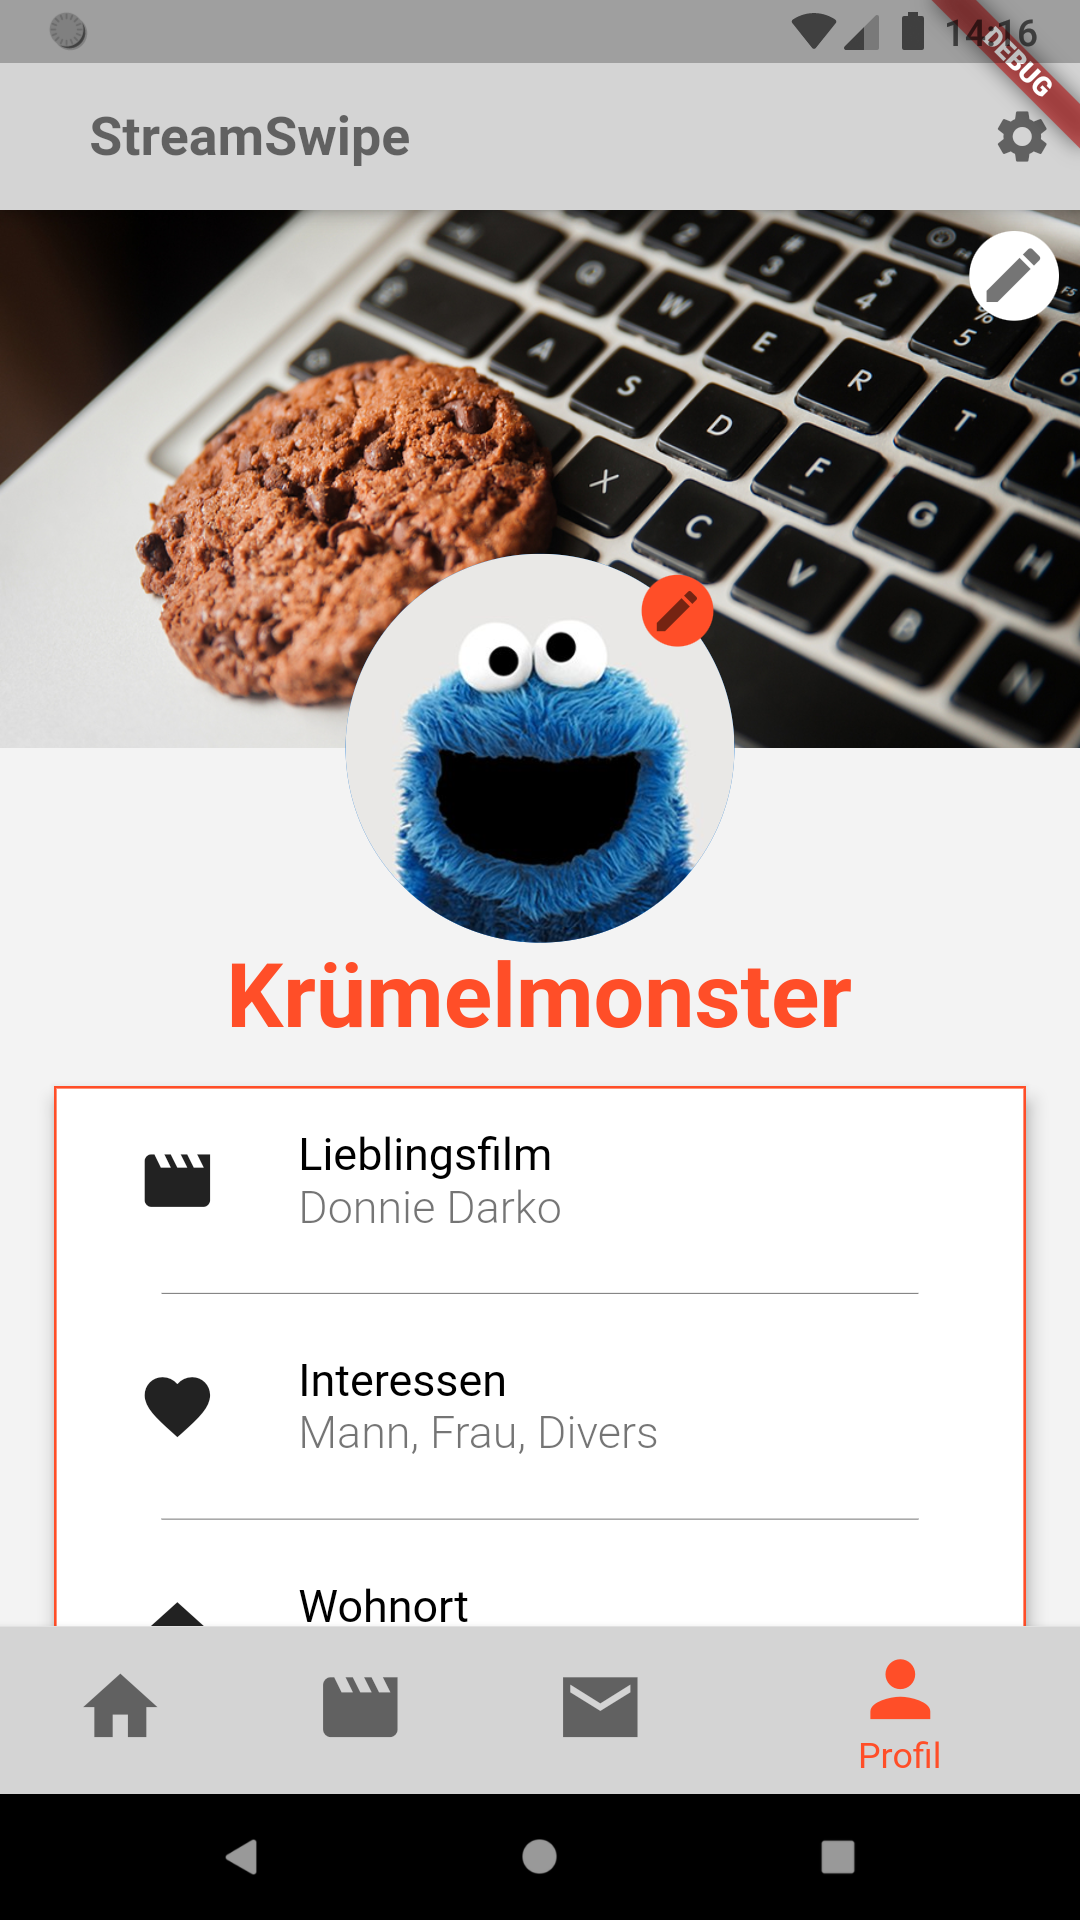
\includegraphics[scale=0.15]{Barrierefreiheit/images/bsp-profil.png}
	\caption{}
	\label{fig:bf-beispiel_b}
	\end{subfigure}
\caption[Screenshots als Beispiele für Barrierefreiheit]{Screenshots aus der App StreamSwipe als Beispiele zu (a) schlichtem Design, bei dem farbige Akzente nicht der Informationenübertragung dienen um die Zugänglichkeit für farbblinde Menschen zu verbessern und für einen Icon in (b), welcher sonst durch sehgeschädigte Menschen nicht wahrnehmbar ist, wird exemplarisch eine Semantik implementiert.}
\label{fig:BF-Beispiele}
\end{figure}


\noindent
Ist die Sehkraft noch weiter eingeschränkt oder gar nicht mehr vorhanden, werden Semantiken eingesetzt. Hierbei erhält jedes Element auf dem Bildschirm eine Beschreibung, die vorgelesen werden kann. Bei Zahlen und Texten werden diese vorgelesen, sofern keine weitere Information hinterlegt ist. Besonders hilfreich ist dies jedoch bei Abbildungen. Ausgeführt wird das Auslesen von einem Screenreader. Mobile Geräte haben diese Funktion bereits standardmäßig eingebaut (VoiceOver bei Apple und TalkBack bei Android) und wandeln die Semantiken mittels Sprachsynthese in akustische Signale um. Bei Desktopanwendungen wie z.B. JAWS für Windows können diese Informationen zusätzlich auch durch eine Braillezeile wiedergegeben werden.\\
Bei Flutter ist das Hinzufügen von Semantiken bereits eingebaut. Hierfür kann ein String dem jeweiligen Bereich zugeordnet werden. In Beispiel \ref{lst:semantics} ist hierfür der Code des Buttons, der zu den Einstellungen führt. In Abbildung \ref{fig:bf-beispiel_b} ist dieser Button ganz rechts oben im Eck zu sehen.\\
Die Funktion \texttt{GestureDetector()} erkennt Interaktionen mit dem Touchscreen, wobei hier nur auf Antippen reagieren soll, deshalb die Funktion \texttt{onTap:()$\{\}$}, die auf den Einstellungsbildschirm leitet. Diese Implementierung ist hier aber nicht von Relevanz und wird übersprungen. In dem \texttt{GestureDetector()} ist ein Icon eingebettet, von der Form \textit{Settings}, was einem Zahnrad entspricht. Dieses Icon erhält eine Farbe und anschließend eine Semantik aus allem was in den Anführungszeichen steht. Ein Screenreader kann AE erkennen und ihn als den Umlaut Ä aussprechen. \\
So wird im kompletten Programm für jedes relevante Element vorgegangen. Teilweise  müssen den Semantiken Variablen übergeben werden, da sich die vorzulesende Information ändert wie beispielsweise bei den Filmtiteln.
    
\begin{lstlisting}[caption=Codeausschnitt in Dart von einem Button mit Semantiken.,label=lst:semantics]
GestureDetector(
  onTap: () {
     ...
  },
  child: Icon(
    Icons.settings,
    color: Provider.of(context).colors.textSmall,
    semanticLabel: "Einstellungen. Zum Auswaehlen doppeltippen.",
  )
),
\end{lstlisting}

\noindent
Bei einer sauberen Implementierung wird auf diese Weise vorgegangen und eine bereits vorhandene Funktion verwendet. Dies vereinfacht nicht nur die Leserlichkeit des Codes, sondern bietet auch die höchste Modularität, da hierbei normalerweise standardisierte Schnittstellen für Betriebssysteme oder andere Anwendungen verwendet werden. In diesem Fall  müssen die Screenreader von Android und Apple damit arbeiten können.\\

\noindent 
Um für Personen mit eingeschränktem Hörvermögen oder vollständiger Gehörlosigkeit die App zugänglich zu machen, wird auf akustisches Feedback als notwendige Infor"-mations"-über"-tragung verzichtet. Innerhalb der App werden keine Geräusche erzeugt, außer der oben beschriebenen Funktion der Semantiken. Beim Erhalten einer neuen Nachricht oder eines neuen Matches kann weiterhin optional eine akustische Benachrichtigung erhalten werden. Hierbei wird die betriebssystemeigene Funktion übernommen, sodass in der App keine neuen Einstellungen vorgenommen werden müssen.\\

\noindent
Auch feinmotorische Einschränkungen werden versucht zu umgehen. Die Navigation und die Filmbewertung in StreamSwipe können durch großflächige Wischbewegungen ausgeführt werden. Wo diese Lösung nicht möglich ist, werden verhältnismäßig große Buttons eingesetzt. Lediglich beim Registrieren und Einloggen werden feine Bewegungen erfordert. Hierbei öffnet sich allerdings die als Standard eingestellte digitale Tastatur, die in vielen Fällen eine Spracheingabe besitzt, sodass die sehr kleinen Tasten nicht benutzt werden müssen.\\

%TODO Diesen Satz evtl. ganz ans Ende ins Fazit
\noindent
Sollte sich in Zukunft jedoch Kritik in Form von negativen Nutzerbewertungen herauskristallisieren, kann eines der noch nicht implementierten Features über ein Update nachgerüstet werden.
\subsection{Oberflächen von StreamSwipe}
\label{sec:UI-alle}
Die Smartphone-App lässt sich in mehrere Bereiche aufteilen, die sich in ihren Funktionen unterscheiden. Auf Basis der oben beschriebenen Grundlagen wurden diese Bereiche entworfen und werden in diesem Kapitel analysiert. Auch wenn manches davon als gewöhnlich oder naheliegend erscheint, so ist jedes Element mit Bedacht gewählt, erstellt und angepasst worden.
\subsubsection{Login-Screen}
\label{sec:loginscreen}
Bei erstmaliger Benutzung der App öffnet sich der Login-Screen. An diesem Punkt wird der erste Eindruck für den Benutzer gesetzt, wobei bei StreamSwipe ein schlichtes Design gewählt wurde. Man sieht helle Grautöne mit einem Akzentfarbton, welche sich durch alle Bildschirme der App ziehen werden. Abhängig davon, ob der User in den Systemeinstellungen den dunklen Modus gewählt hat, werden anstatt den hellen Grautönen, dunkle bis schwarze Farben dargestellt, siehe auch Abbildungen \ref{fig:homescreen_c} und \ref{fig:swipescreen_e}.\\
Auf dem Login-Screen (siehe Abbildung \ref{fig:login_a}) sind neben einer Überschrift mehrere beschriftete Textfelder und Buttons zu sehen, welche allesamt mit Semantiken versehen wurden, um durch einen Screenreader erkannt und identifiziert werden zu können. Die gewählte Anordnung wird universell bei Apps, Programmen und Webseiten benutzt, sodass die Felder auch ohne die eingetragenen Hinweistexte korrekt ausgefüllt werden könnten. Beim Antippen der Textfelder, öffnet sich die Standardtastatur des Betriebssystems. Sind alle Felder korrekt ausgefüllt, wird der User in die eigentliche App weitergeleitet, ansonsten wird durch individualisierte Fehlermeldung auf eventuelle Falscheingaben hingewiesen. Nach Erstellen eines neuen Accounts, durchläuft der User einen ähnlich aufgebauten Bildschirm (siehe Abbildung \ref{fig:login_b}) und wird danach aufgefordert weitere Informationen zur Profilvervollständigung einzugeben (siehe Abbildung \ref{fig:login_c} und \ref{fig:login_d}). Auch hierbei werden bekannte Bedienelemente wie Textfelder, Dropdownmenüs und Checkboxen verwendet, wie in den Abbildungen \ref{fig:login_e} und \ref{fig:login_f} beispielhaft dargestellt sind.


\begin{figure}[tbt]
	\begin{subfigure}{0.33\textwidth}
	\centering
	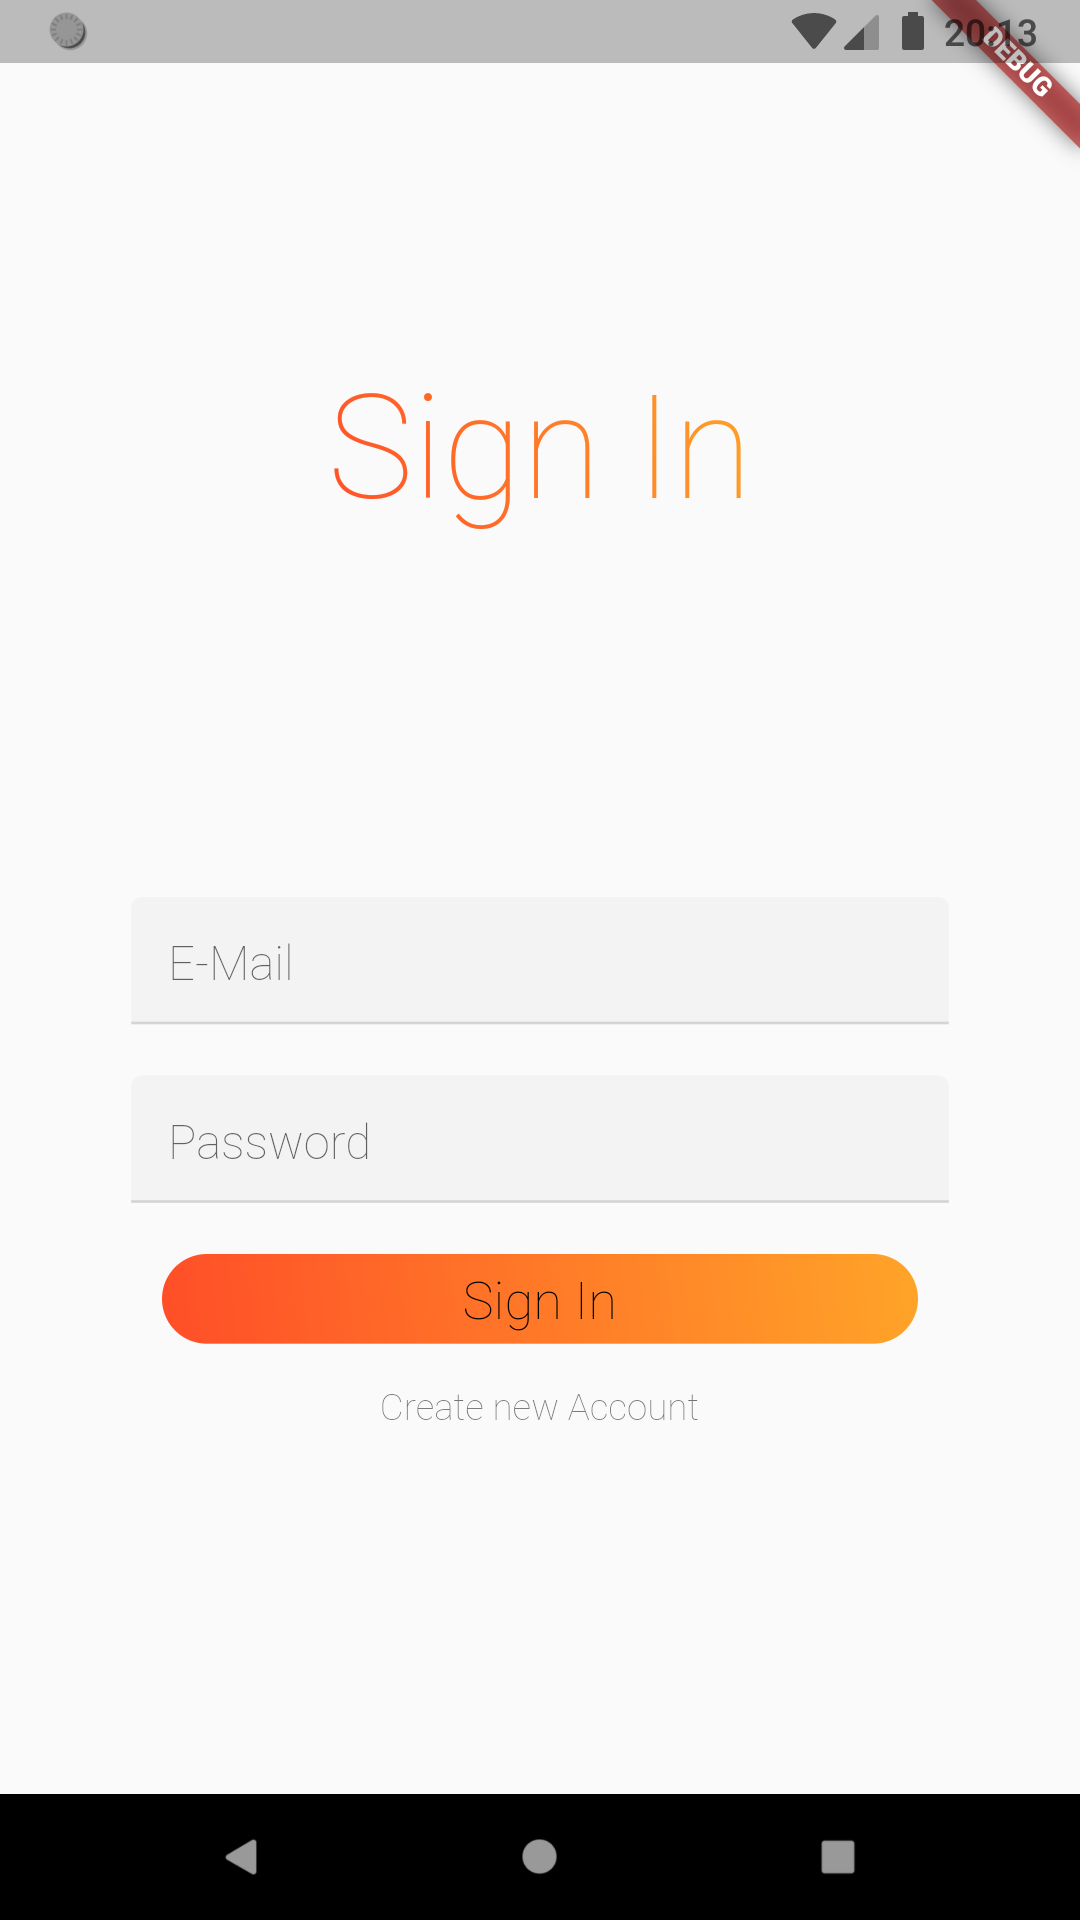
\includegraphics[scale=0.13]{Benutzeroberfläche/images/screenshot_login_1.png}
	\caption{}
	\label{fig:login_a}
	\end{subfigure}
	\begin{subfigure}{0.33\textwidth}
	\centering
	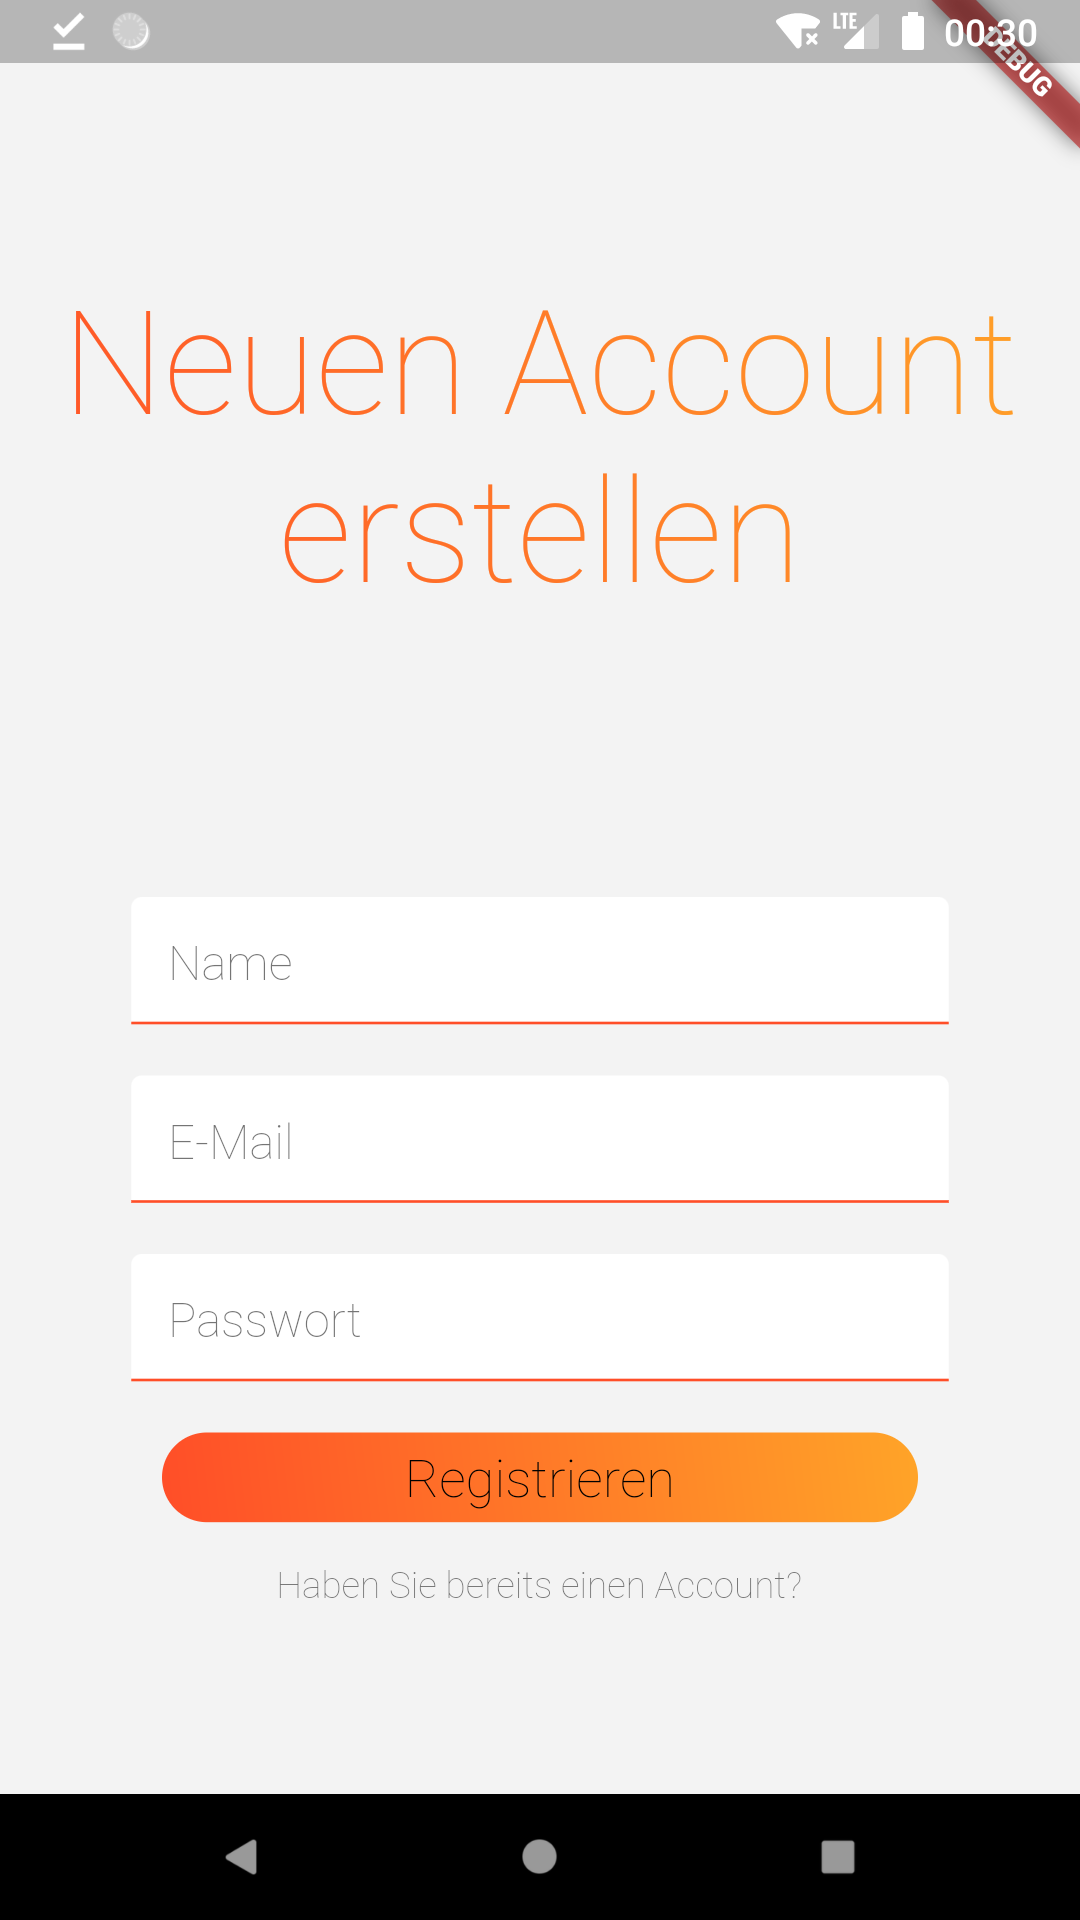
\includegraphics[scale=0.13]{Benutzeroberfläche/images/screenshot_login_2.png}
	\caption{}
	\label{fig:login_b}
	\end{subfigure}
	\begin{subfigure}{0.33\textwidth}
	\centering
	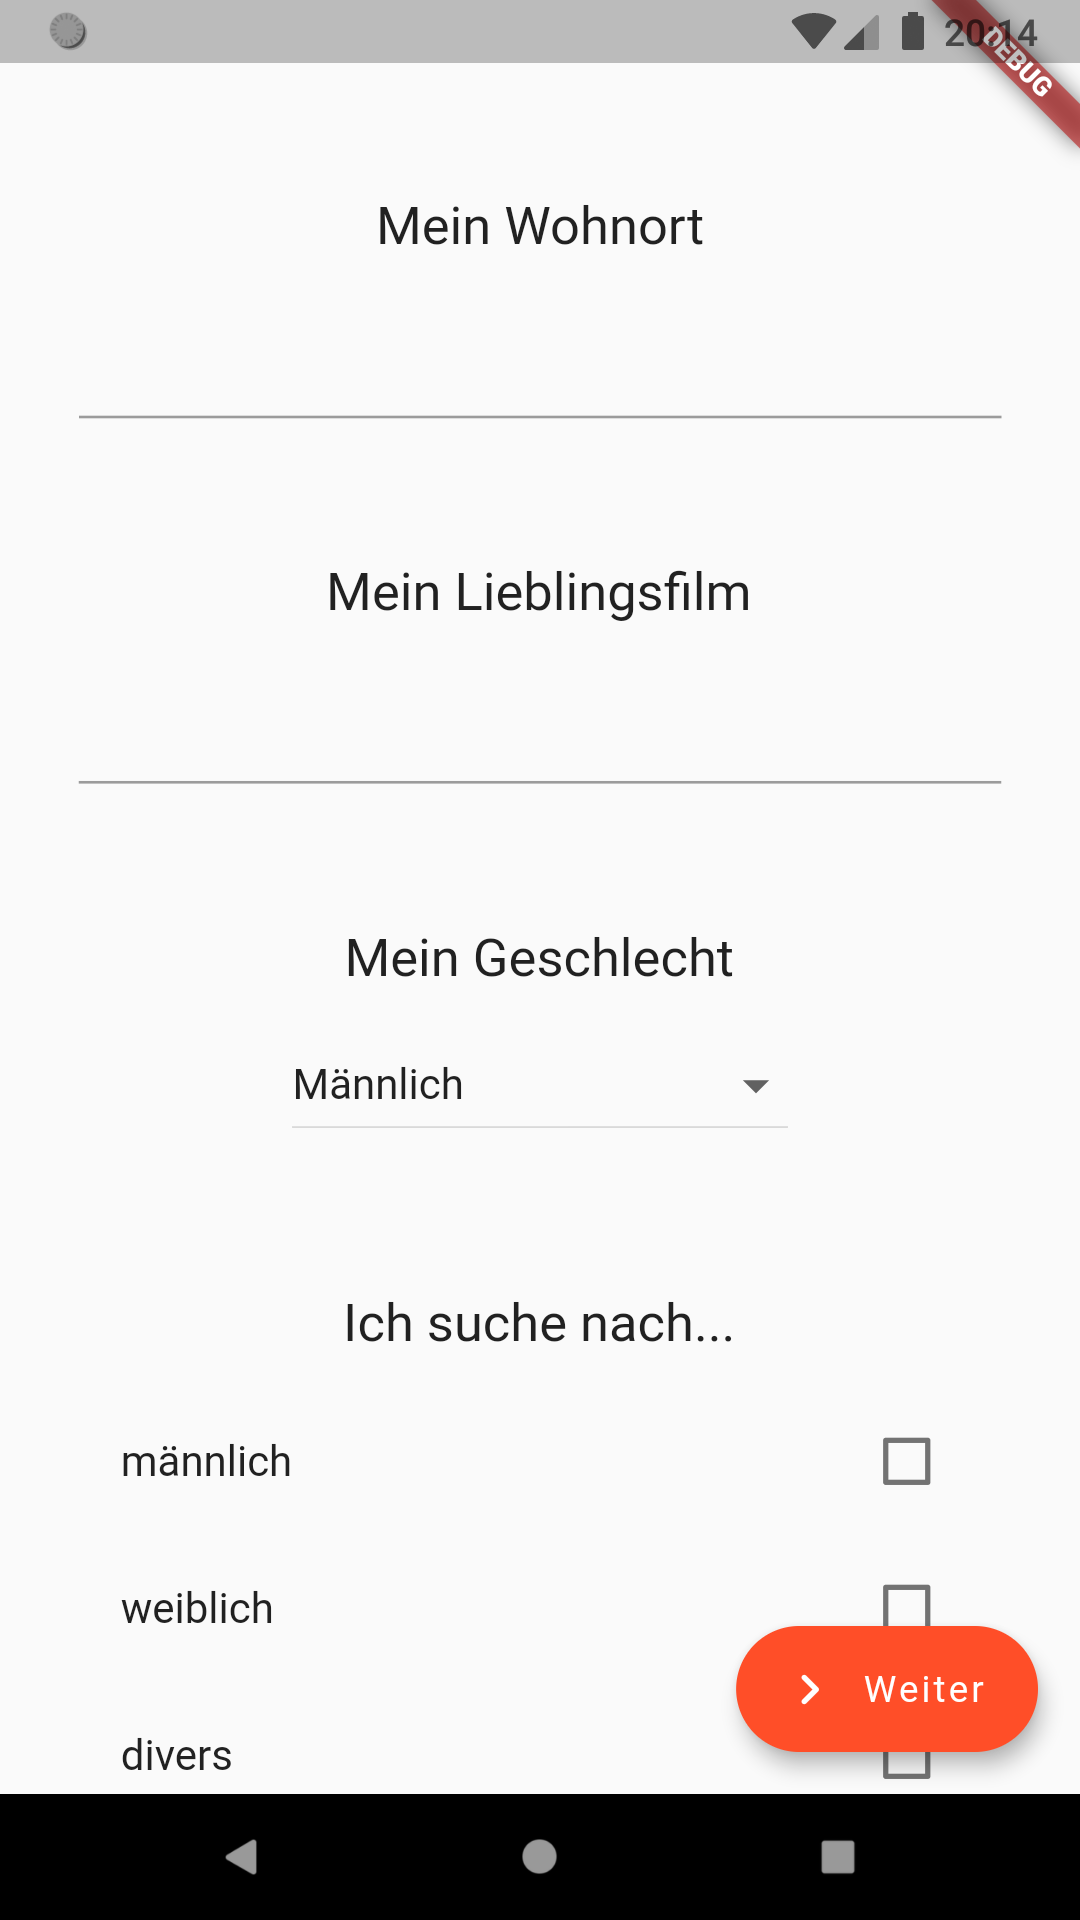
\includegraphics[scale=0.13]{Benutzeroberfläche/images/screenshot_login_3.png}
	\caption{}
	\label{fig:login_c}
	\end{subfigure}\\ \vspace{1cm}	
	
	\begin{subfigure}{0.33\textwidth}
	\centering
	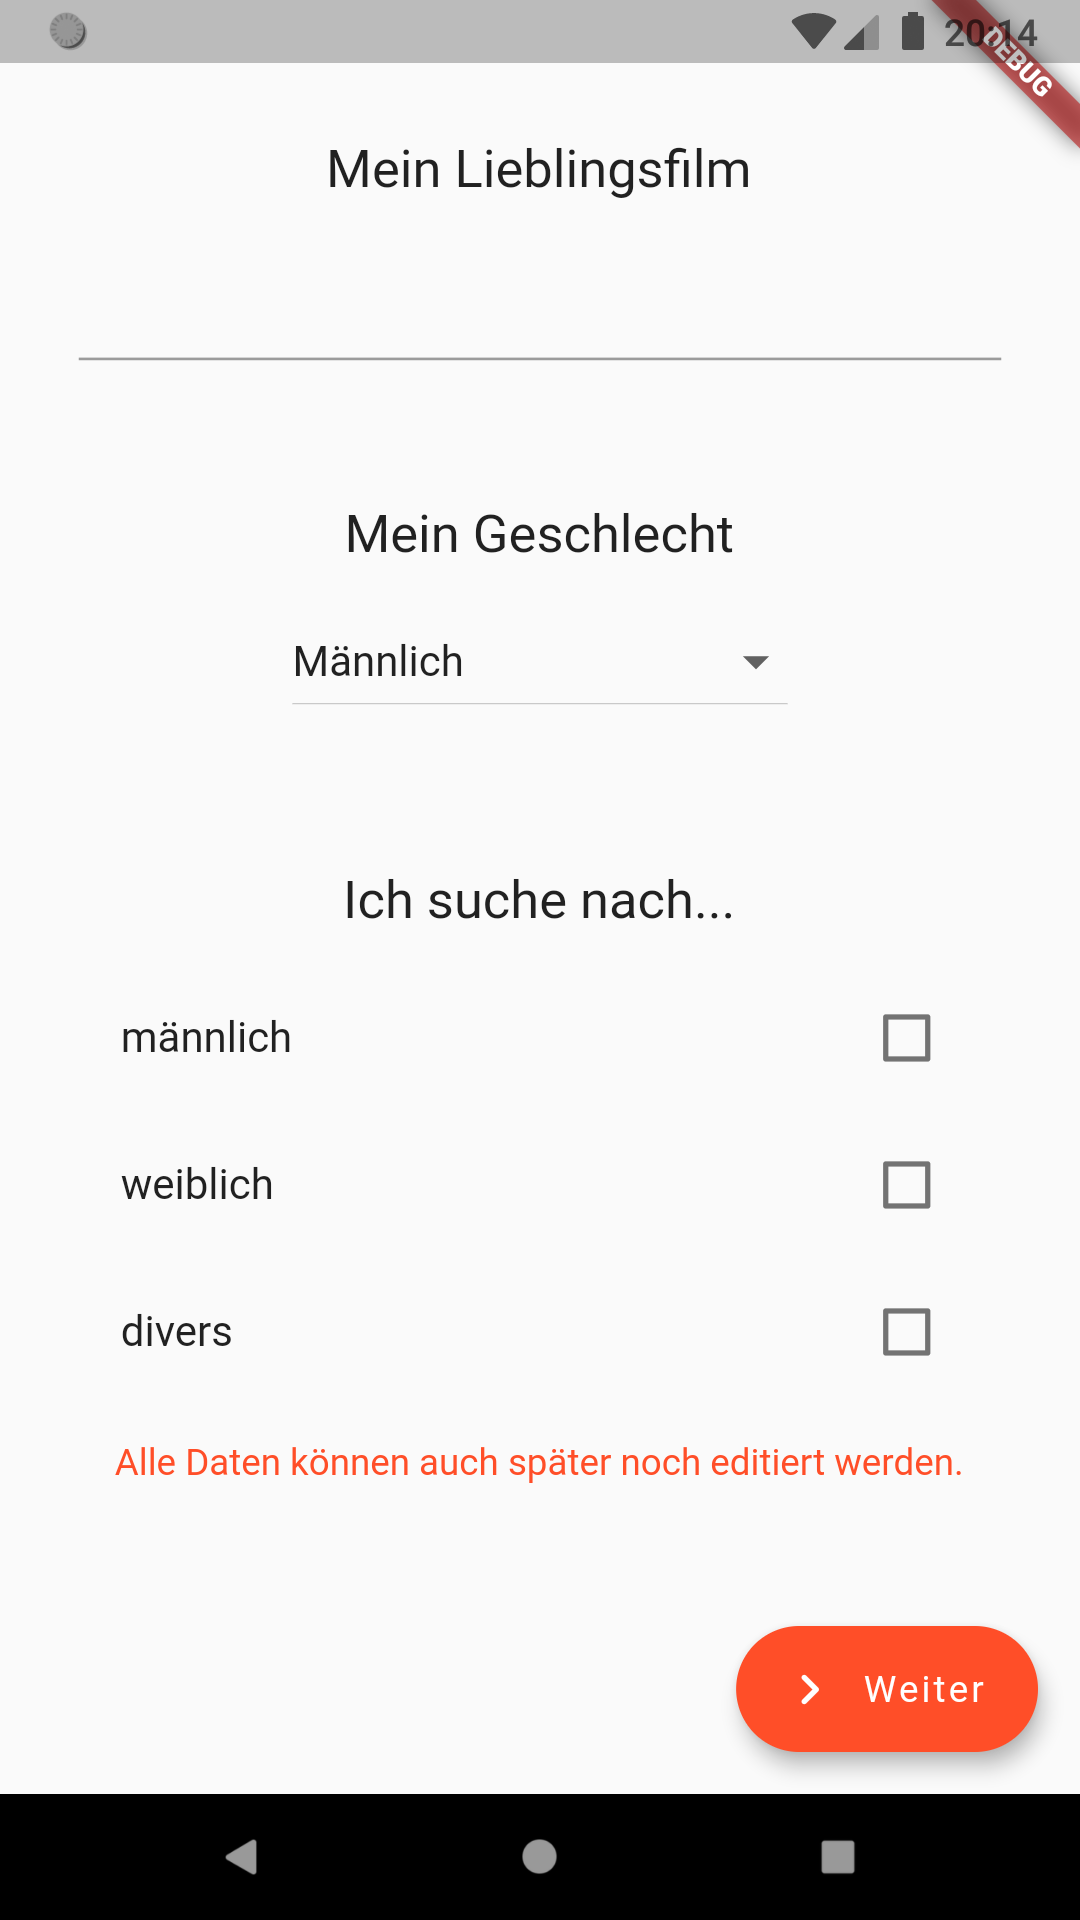
\includegraphics[scale=0.13]{Benutzeroberfläche/images/screenshot_login_4.png}
	\caption{}
	\label{fig:login_d}
	\end{subfigure}
	\begin{subfigure}{0.33\textwidth}
	\centering
	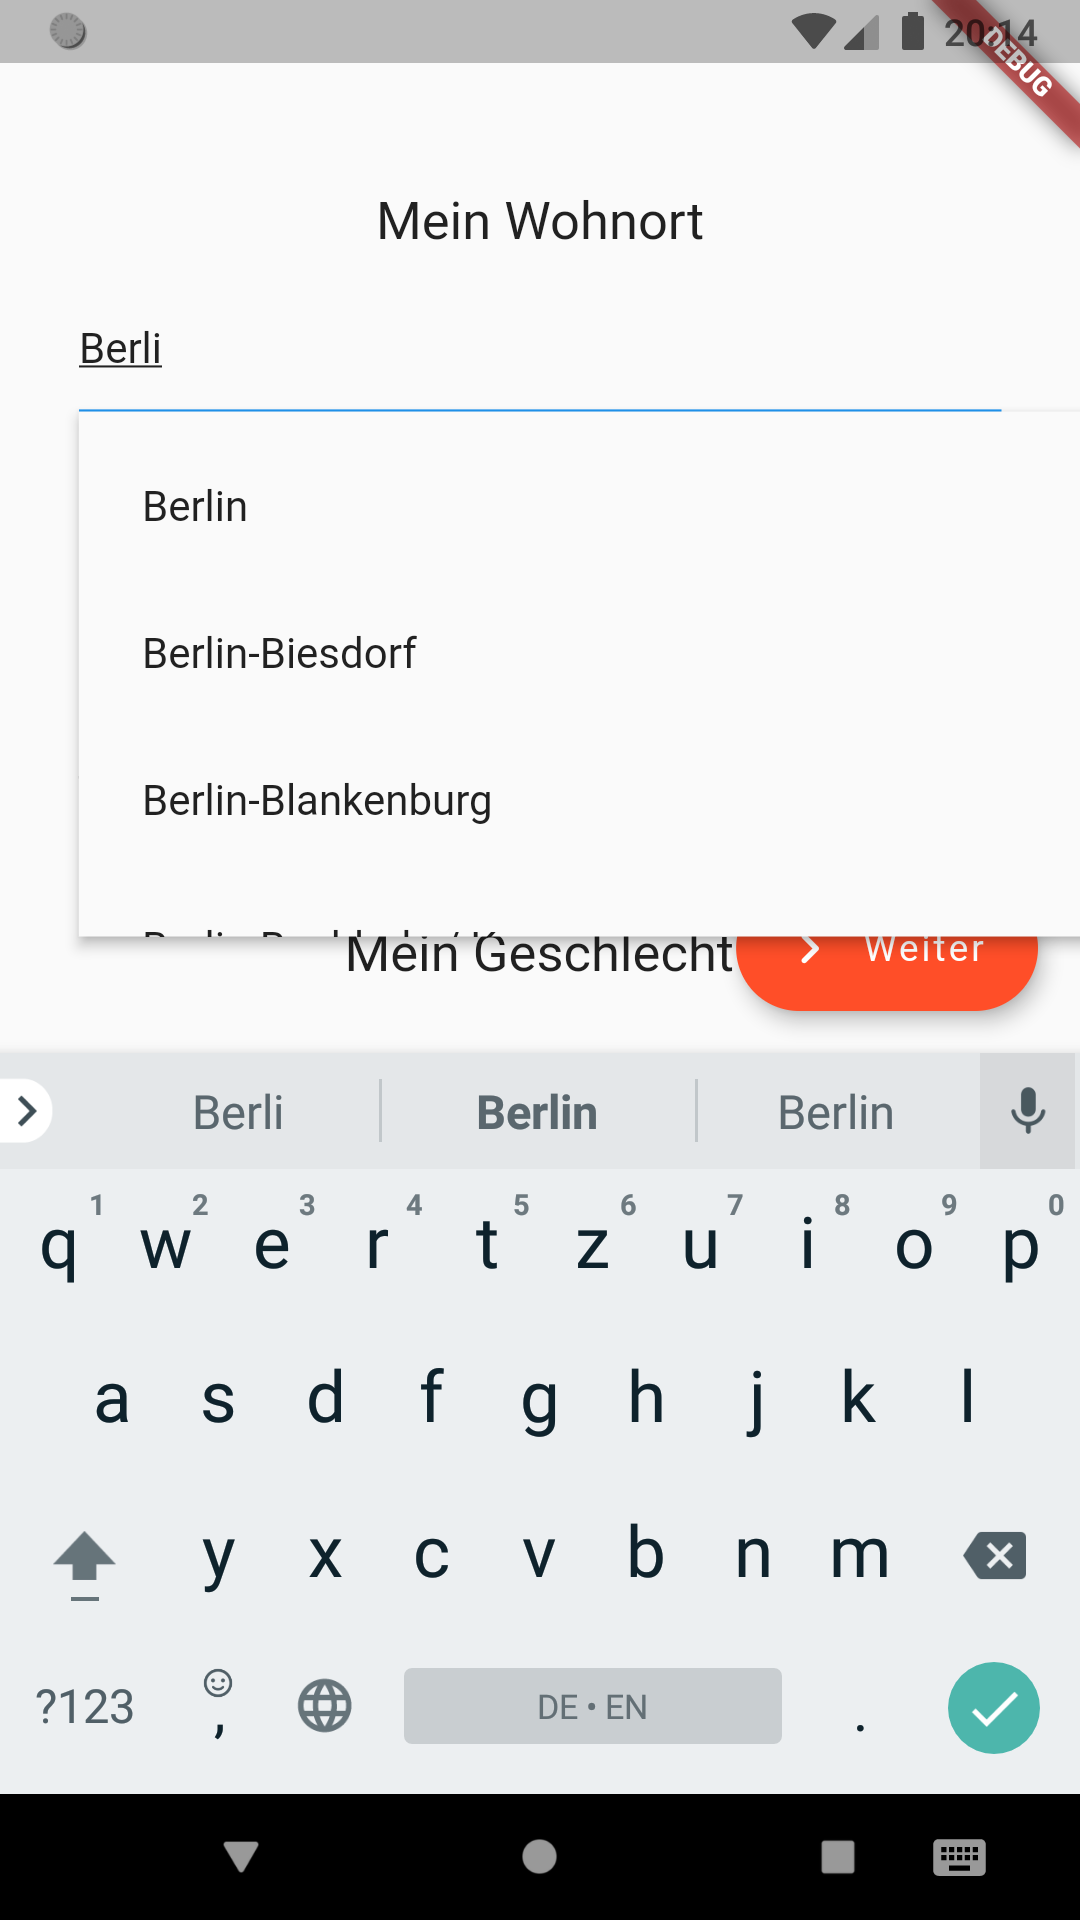
\includegraphics[scale=0.13]{Benutzeroberfläche/images/screenshot_login_5.png}
	\caption{}
	\label{fig:login_e}
	\end{subfigure}
	\begin{subfigure}{0.33\textwidth}
	\centering
	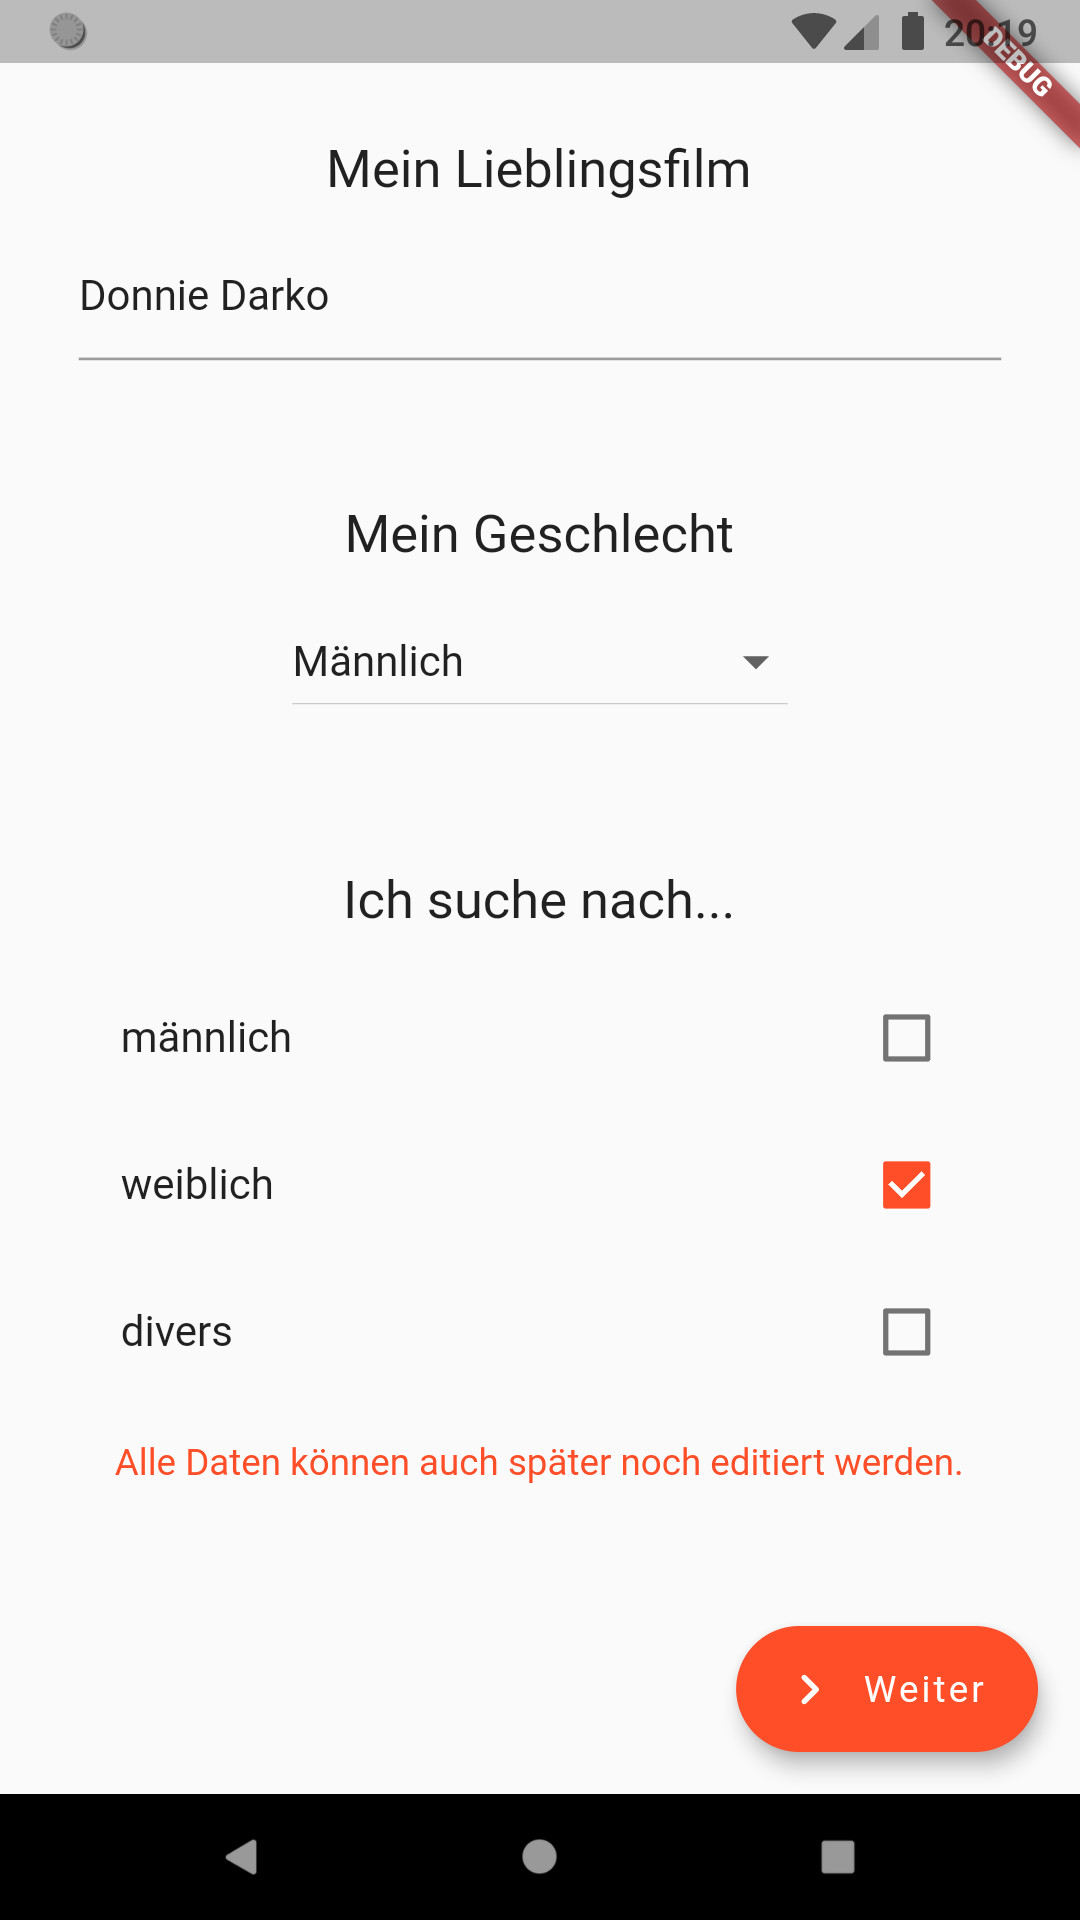
\includegraphics[scale=0.13]{Benutzeroberfläche/images/screenshot_login_6.png}
	\caption{}
	\label{fig:login_f}
	\end{subfigure}
\caption{Der Login-Screen von StreamSwipe und alle damit zusammenhängenden Seiten. Man sieht (a) das Einloggen bei bestehendem Account, (b) das Erstellen eines Accounts, (c) und (d) das Formular für die weiter benötigten Profildaten, (e) Ein Texteingabefeld mit Autovervollständigung als Dropdownmenü und (f) eine ausgefüllte Formular.}
\label{fig:login_alle}
\end{figure}
\clearpage

\subsubsection{Home-Screen}
\label{sec:homescreen}

Da davon ausgegangen wird, dass der User sich nicht nach jeder Nutzung ab- und wieder anmeldet, erscheint im alltäglichen Gebrauch der in Abbildung \ref{fig:homescreen_alle} dargestellte Bildschirm zuerst. Demnach bietet es sich an Ereignisse wie neue Matches und neue Nachrichten hier anzuzeigen. Diese werden wie Abbildungen \ref{fig:homescreen_a} und \ref{fig:homescreen_b} zeigen klar strukturiert in Abschnitte eingegliedert, welche mit Überschriften kenntlich gemacht sind. Die einzelnen Matches befinden sich mit allen dazugehörenden Funktionen und Informationen jeweils auf einer Karte. Durch diese Karten kann mit einer von anderen \mbox{Apps} bekannten horizontalen Swipemechanik navigiert werden. Weiterführende Funktionen wie das Starten eines Chats oder das Löschen des Matches werden durch  Antippen von allgemein verständlichen Icons ausgeführt. \\
Auch auf diesem Screen findet sich einerseits das bereits eingeführte Farbschema wieder und es werden andererseits ebenfalls Semantiken verwendet. Bei den neuen Nachrichten wird jeweils der Benutzername vorgelesen und bei den neuen Matches je nach ausgewähltem Bereich der Filmname, die Icons oder der Text dazwischen.\\
Am unteren Bildschirmrand ist eine sogenannte Bottom-Navigation-Bar zu sehen. Sie ermöglicht eine kompakte und anschauliche Navigation durch die relevanten Bildschirme. Außerdem zeigt sie an welcher Bildschirm aktuell ausgewählt ist. Liest der Screenreader die Semantik hiervon, gibt er die Bezeichnung des aktuellen Bildschirms sowie die Anzahl der weiteren Möglichkeiten an. \\
%TODO Motorische Herausforderungen!!! Anklicken des Filmposters aktiviert auch Chat?

\begin{figure}[tbt]
	\begin{subfigure}{0.33\textwidth}
	\centering
	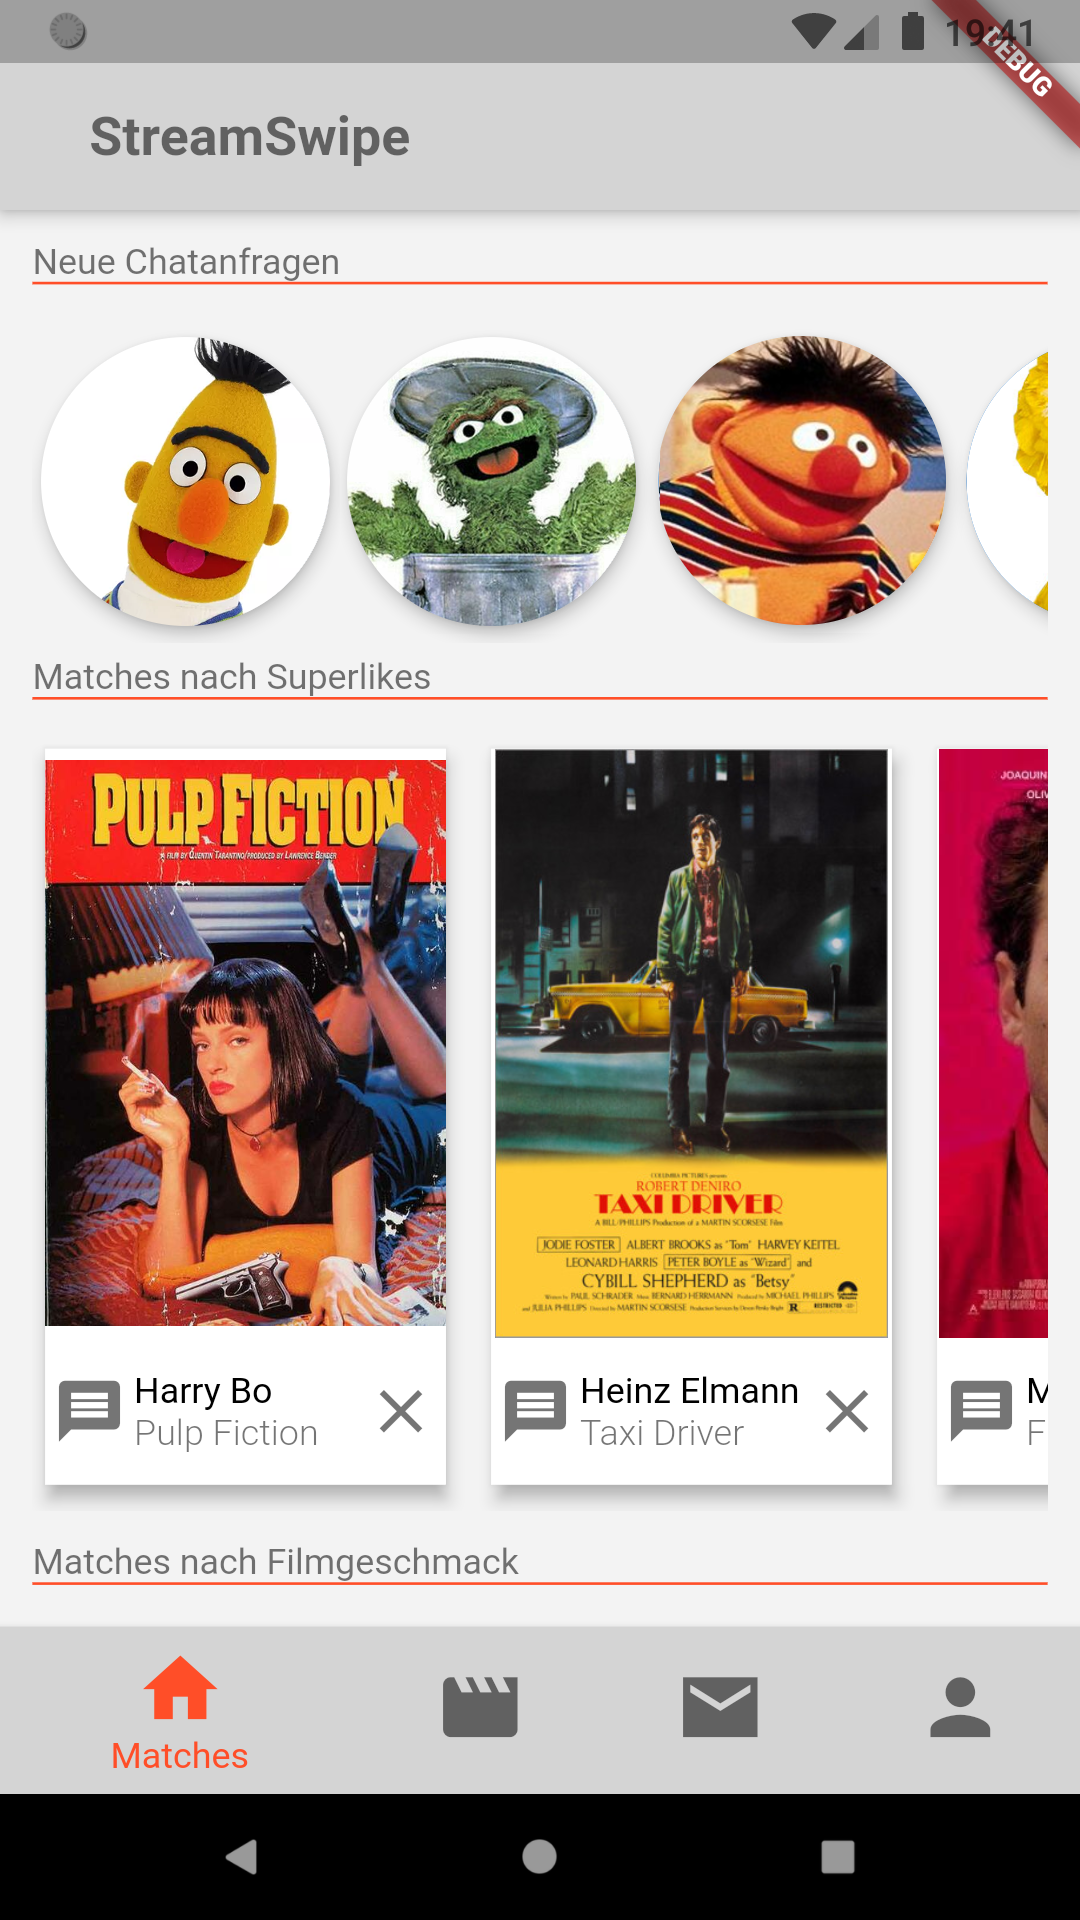
\includegraphics[scale=0.13]{Benutzeroberfläche/images/screenshot_homescreen_1.png}
	\caption{}
	\label{fig:homescreen_a}
	\end{subfigure}
	\begin{subfigure}{0.33\textwidth}
	\centering
	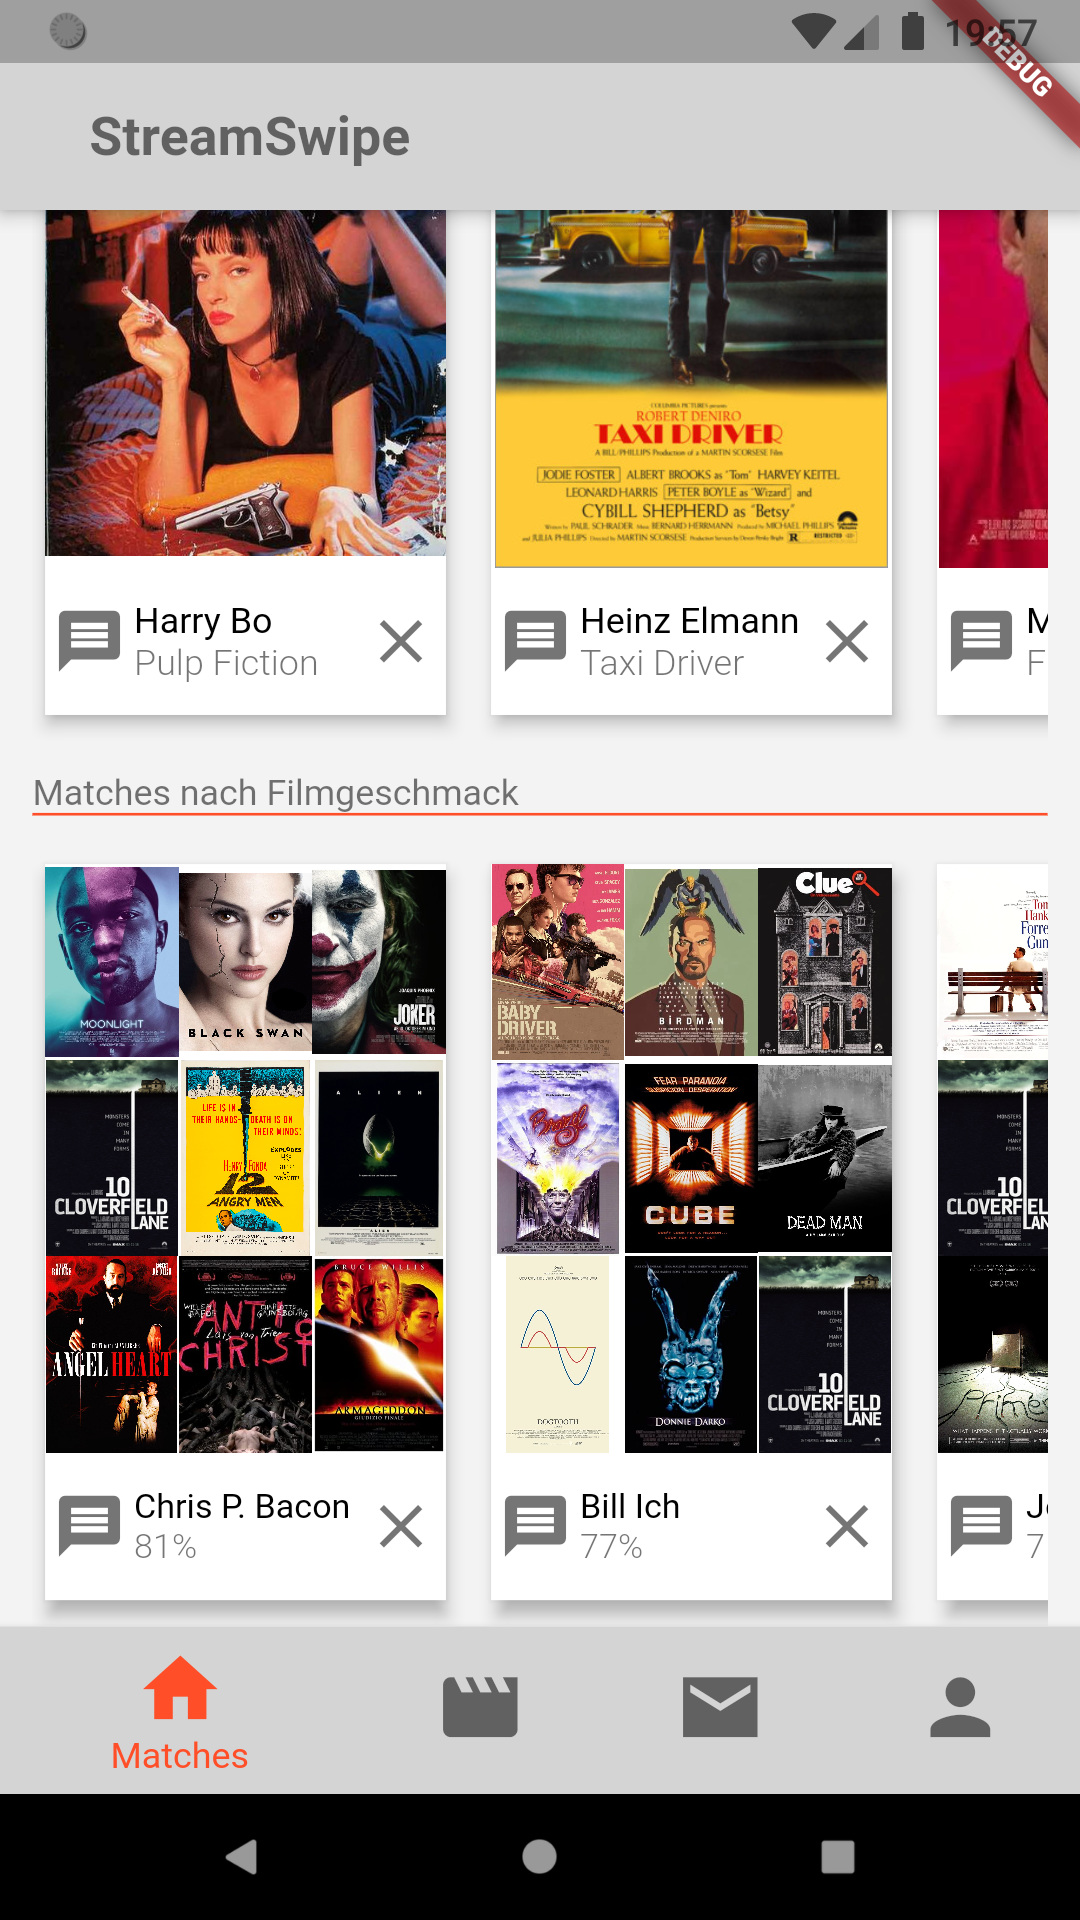
\includegraphics[scale=0.13]{Benutzeroberfläche/images/screenshot_homescreen_2.png}
	\caption{}
	\label{fig:homescreen_b}
	\end{subfigure}
	\begin{subfigure}{0.33\textwidth}
	\centering
	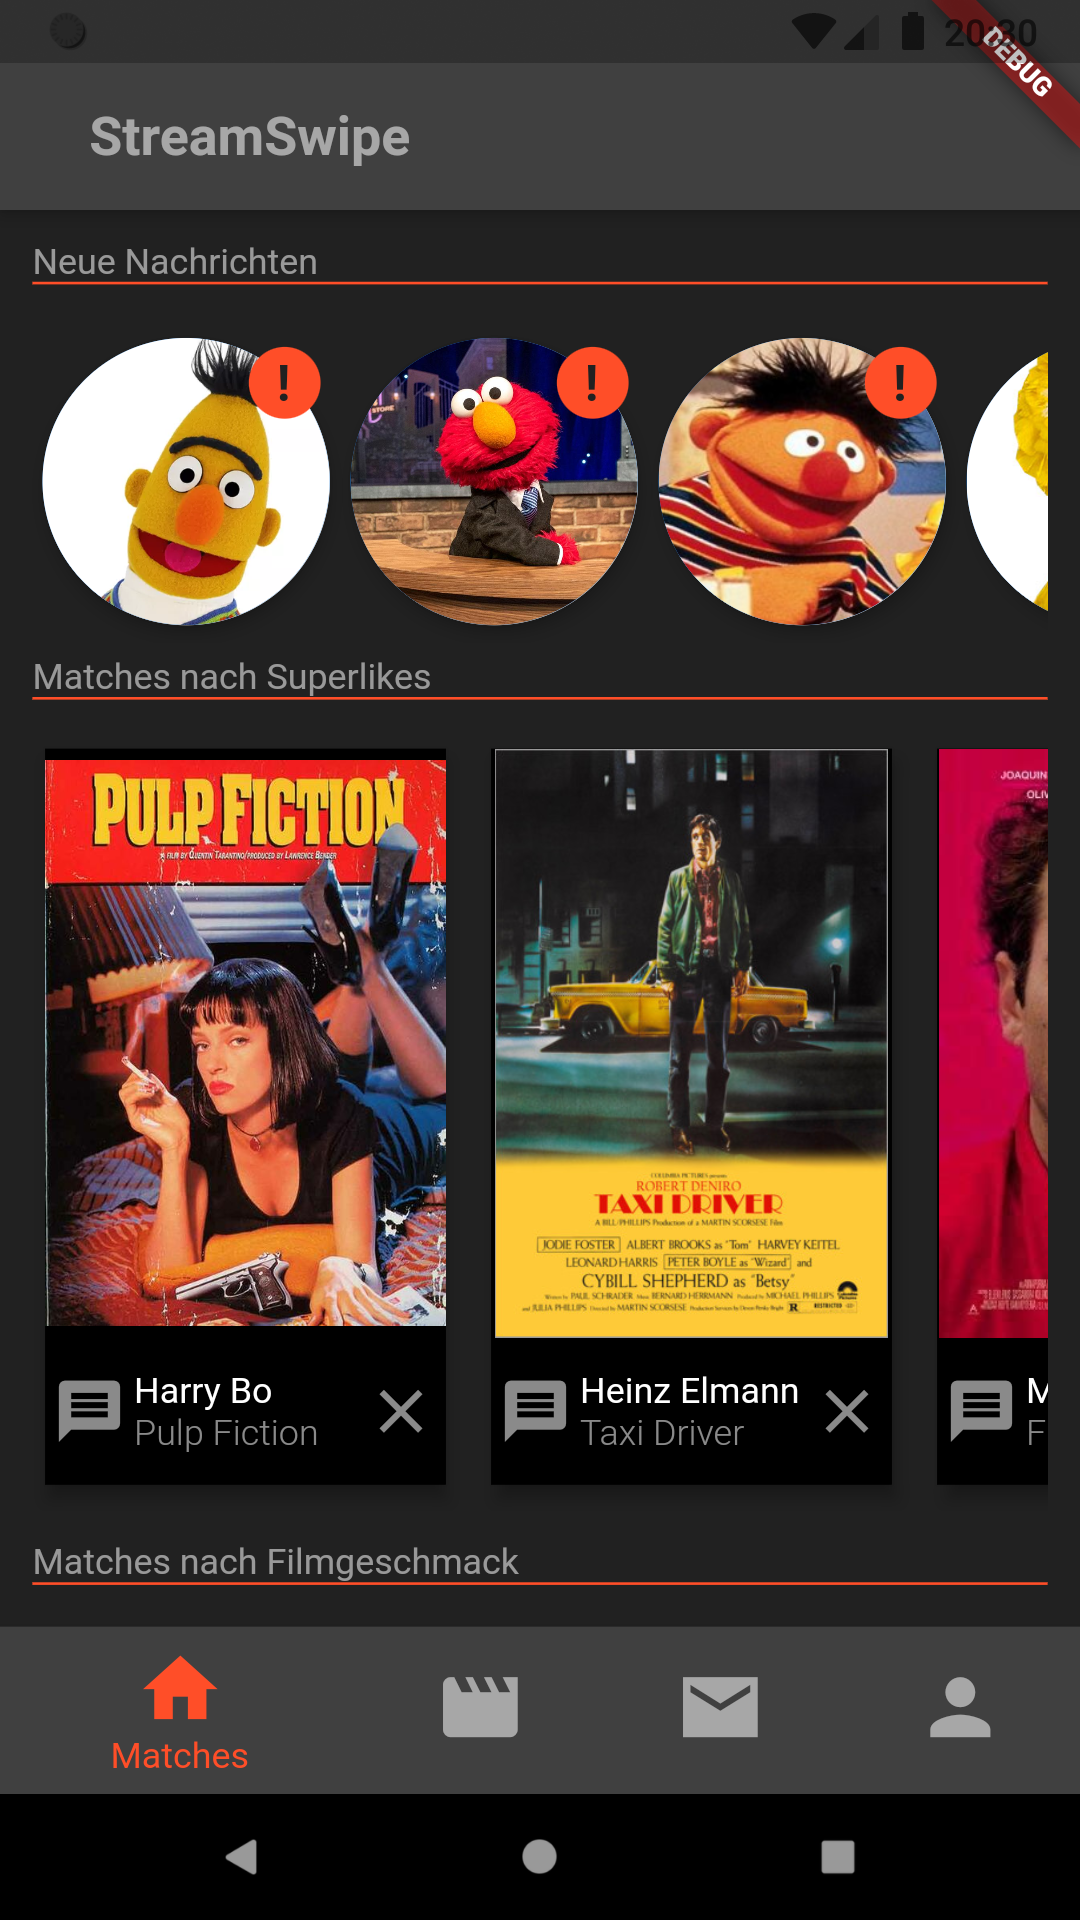
\includegraphics[scale=0.13]{Benutzeroberfläche/images/screenshot_darkmode_1.png}
	\caption{}
	\label{fig:homescreen_c}
	\end{subfigure}
\caption{Der Home-Screen, der beim Öffnen der App zuerst gezeigt wird und Neuigkeiten wie neue Nachrichten und Matches zusammenfasst. Um den gesamten Inhalt dieser Seite sehen zu können, wird in (a) der obere Abschnitt und in (b) der untere Abschnitt gezeigt. Hat der User in den Systemeinstellungen den dunklen Modus aktiviert, so wird (c) der Home-Screen wie alle anderen Screens angepasst.}
\label{fig:homescreen_alle}
\end{figure}


\subsubsection{Swipe-Screen}
\label{sec:swipescreen}
Auf dem Swipe-Screen (Abbildungen \ref{fig:swipescreen_alle}) findet die Bewertung der Filme statt. Durch das hier verwendete Matchingsystem mithilfe des Filmgeschmacks unterscheidet sich StreamSwipe von anderen Apps und erhält so einen innovativen, individuellen Charakter, womit diese Seite das Herzstück der App bildet.\\
Das zuvor eingeführte Farbschema bleibt auch hier erhalten, wie Abbildung \ref{fig:swipescreen_a} zeigt. Eine Überschrift im selben Stil wie bereits aus Abschnitt \ref{sec:homescreen} bekannt, verdeutlicht durch eine Frage nach welcher Motivation die Filmauswahl getroffen werden soll. Zentral im Bild ist eine Liste von Postern der zu beurteilenden Filme. Wie bereits durch die Datingapp Tinder verbreitet, werden die vier Antwortmöglichkeiten durch eine Swipe-Bewegung in eine der vier Richtungen ausgewählt. Abhängig von der Position des Fingers auf dem Touchscreen bewegt sich das Filmposter innerhalb des Bildschirms, was den Effekt einer frei beweglichen Karte hervorruft. Um klarzustellen welche Swipe-Richtung für welche Entscheidung steht, verfärbt sich der jeweilige Indikator in der unteren Reihe bei Verschiebung des Filmposter. Beide diese Animationen sind in Abbildung \ref{fig:swipescreen_d} zu sehen. Die Indikatoren sind mit Icons versehen, zeigen aber durch Drücken welche Entscheidung sie repräsentieren und in welche Richtung der User dafür swipen muss, wie Abbildung \ref{fig:swipescreen_c} am Beispiel des rechten Indikators zeigt. \\
Durch Antippen des Filmposters werden weitere Informationen zu dem jeweiligen Film dargestellt, wie in Abbildung \ref{fig:swipescreen_b} zu sehen. Gleichfalls wird durch ein einfaches Antippen wieder zurück  zu den Postern gewechselt. Eine Rotations-Animation verdeutlicht die Illusion der Karten.\\
Alle diese für die Bedienung der App grundlegenden Steuerungen verlangen keine feinmotorischen Eingaben und können problemlos von Personen mit motorischen Einschränkungen genutzt werden. Auch dieser Bildschirm ist vollkommen mit Semantiken ausgestattet. Anstelle des Filmposters wird der Name des Films ausgelesen und für die vier Indikatoren am unteren Rand werden jeweils deren Funktion und durch welche Swipe-Richtung sie erreicht werden vorgelesen. Sämtliche Textfelder können ebenfalls problemlos von einem Screenreader gelesen werden.



\begin{figure}[tbt]
	\begin{subfigure}{0.33\textwidth}
	\centering
	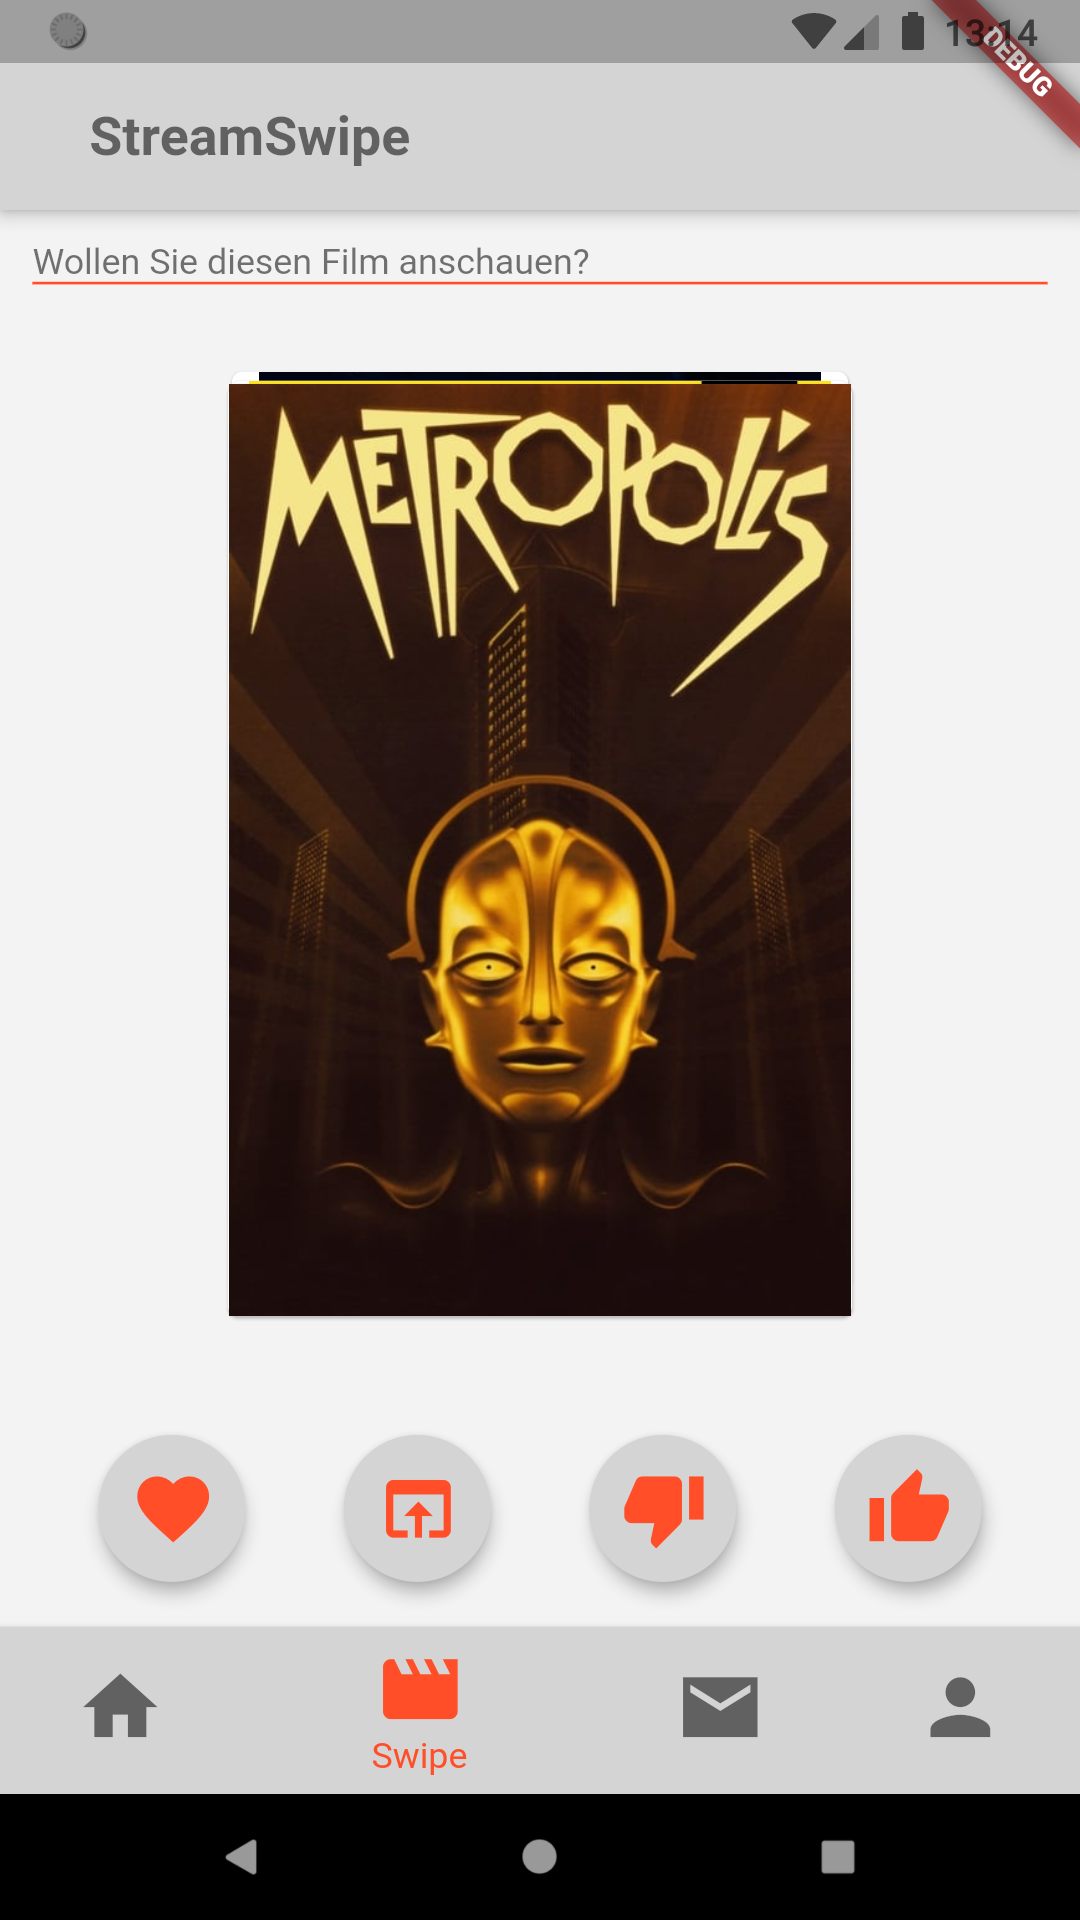
\includegraphics[scale=0.13]{Benutzeroberfläche/images/screenshot_swipescreen1.png}
	\caption{}
	\label{fig:swipescreen_a}
	\end{subfigure}
	\begin{subfigure}{0.33\textwidth}
	\centering
	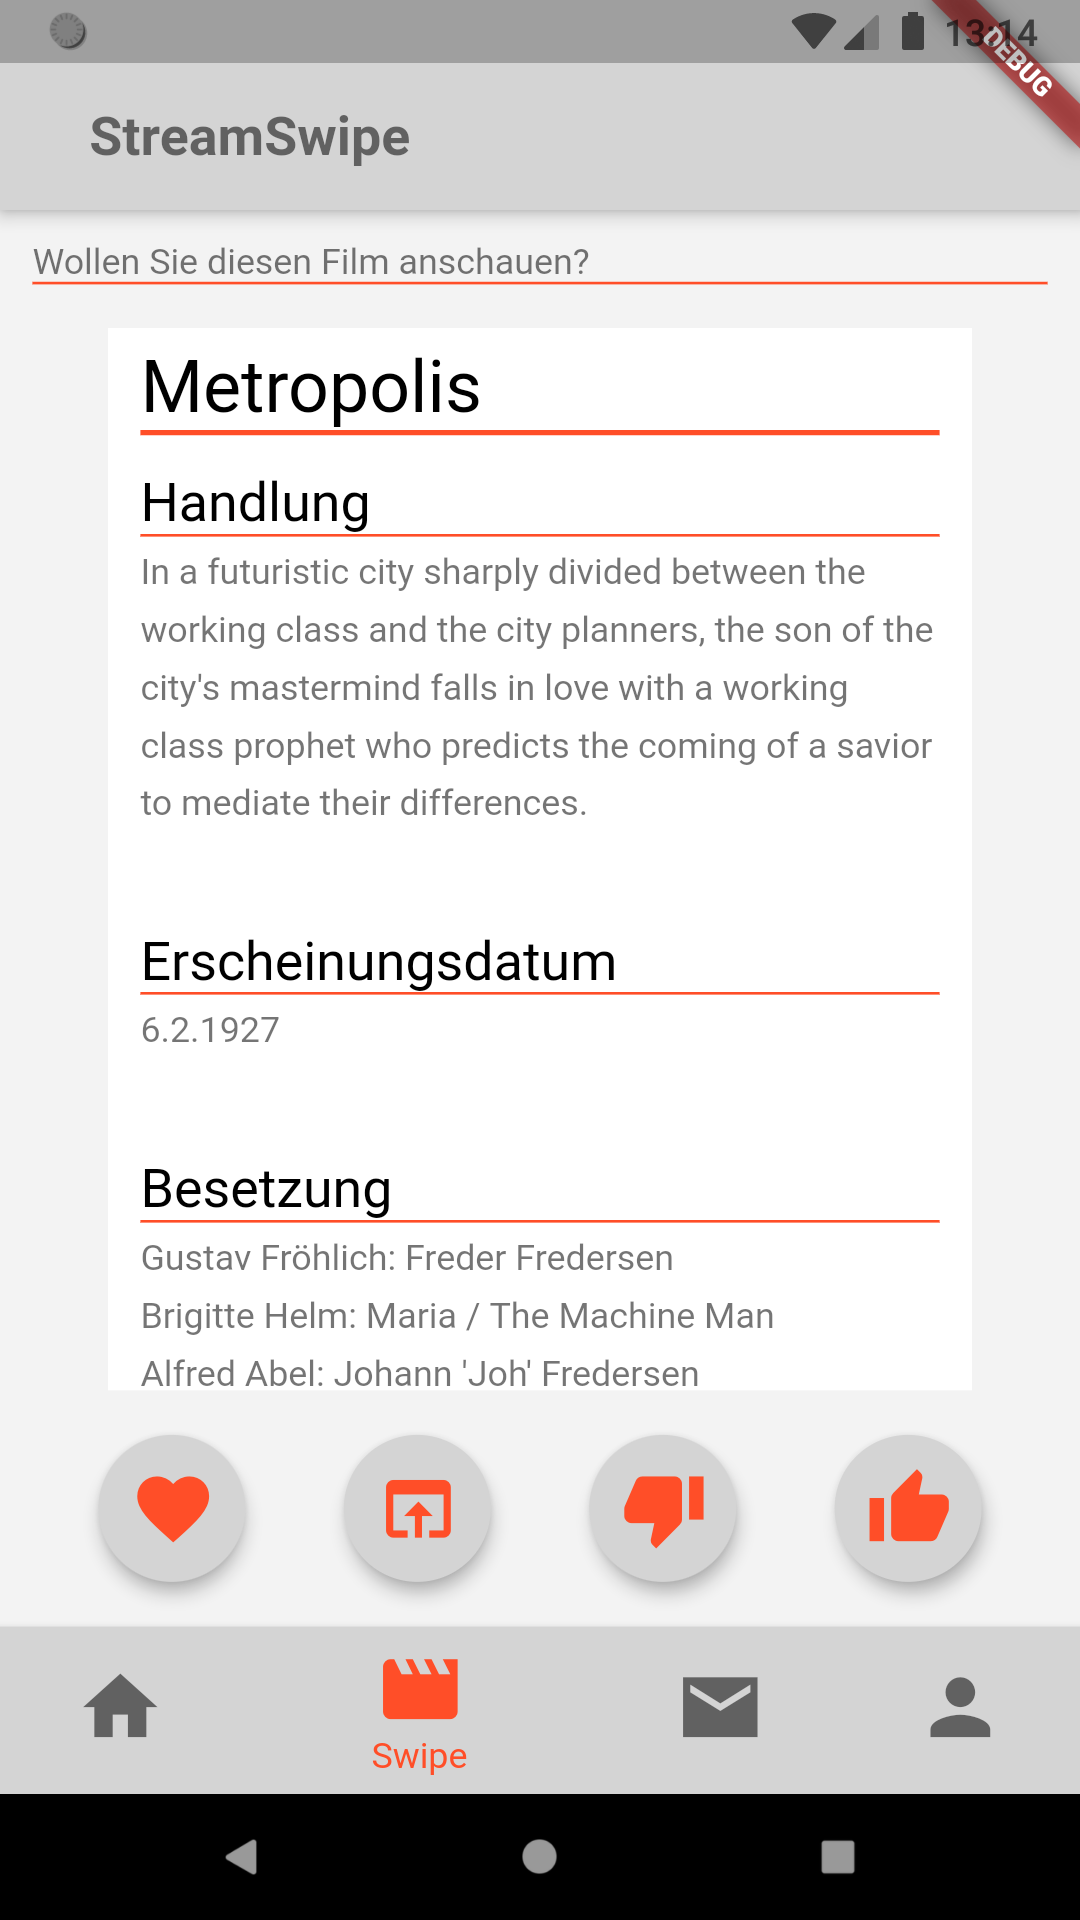
\includegraphics[scale=0.13]{Benutzeroberfläche/images/screenshot_swipescreen2.png}
	\caption{}
	\label{fig:swipescreen_b}
	\end{subfigure}
	\begin{subfigure}{0.33\textwidth}
	\centering
	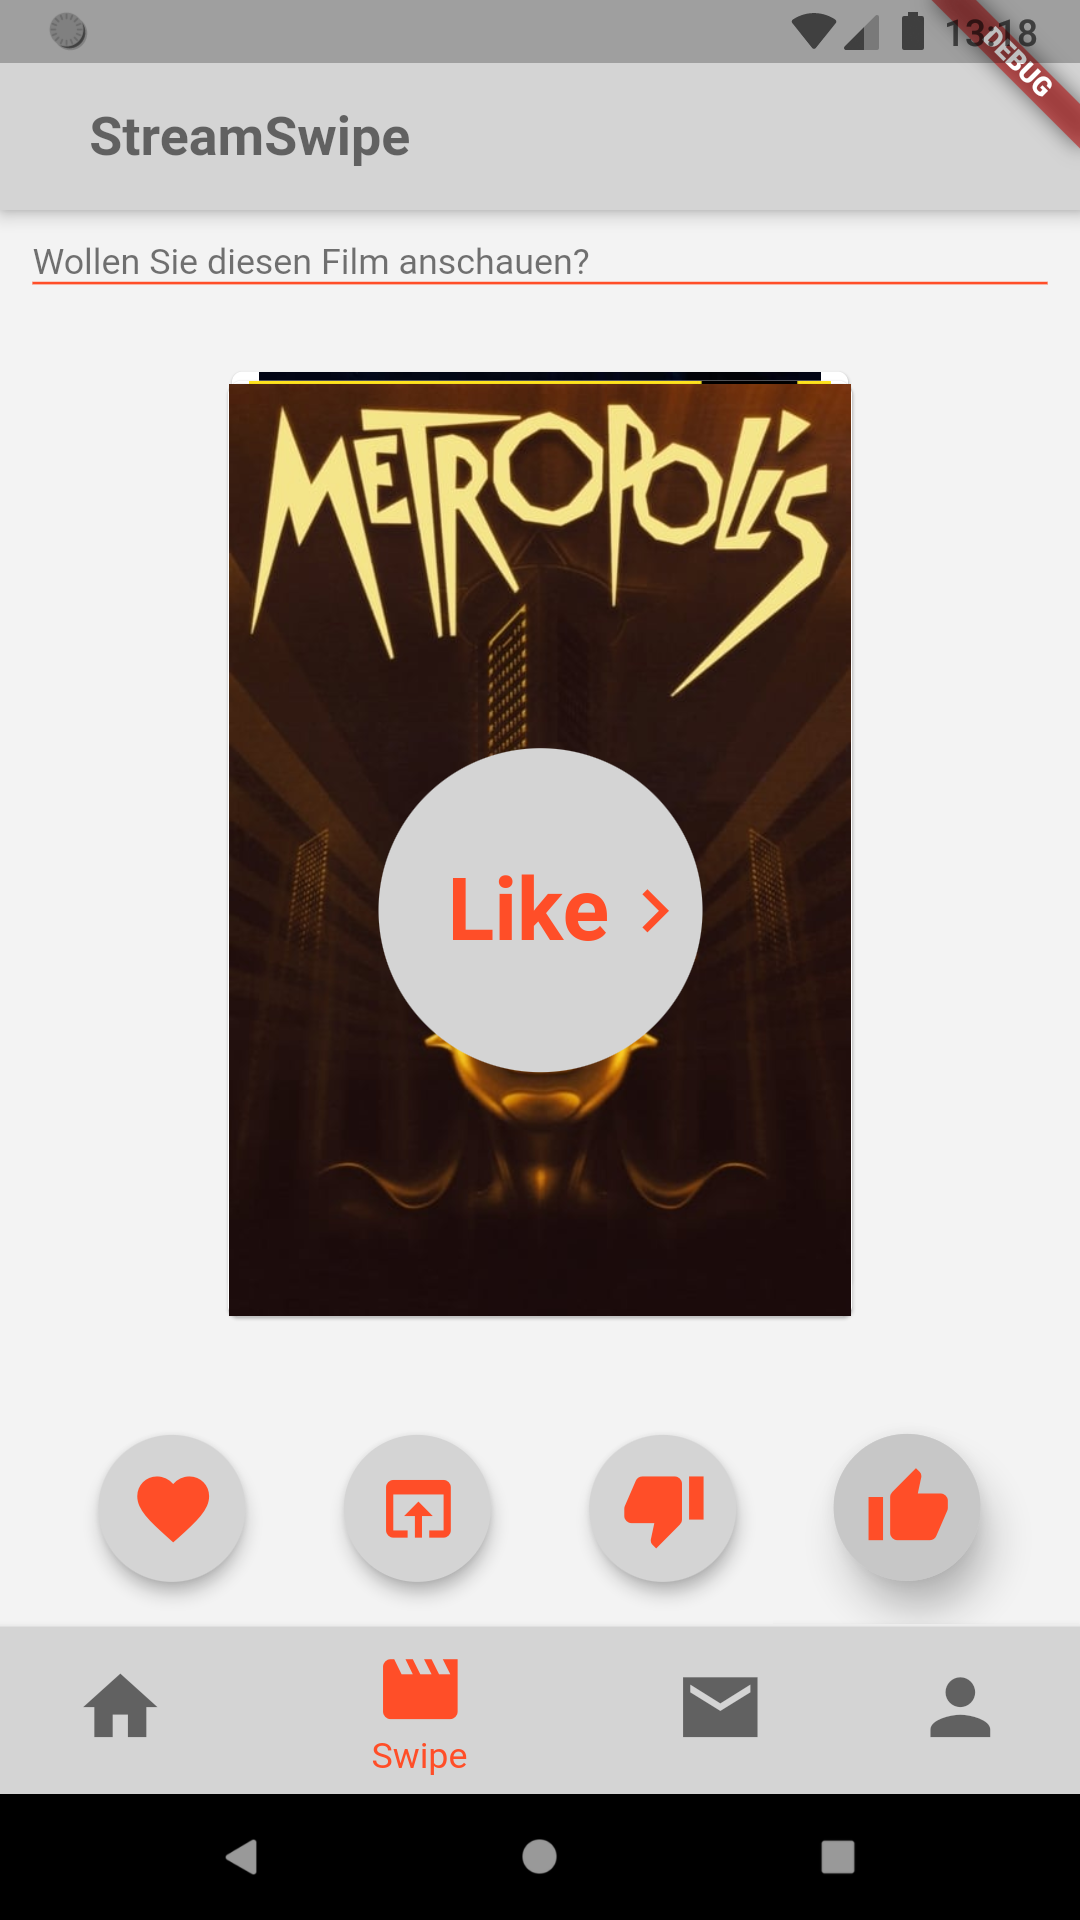
\includegraphics[scale=0.1742]{Benutzeroberfläche/images/screenshot_swipescreen3.png}
	\caption{}
	\label{fig:swipescreen_c}
	\end{subfigure}\\ \vspace{1cm}	
	
	\begin{subfigure}{0.33\textwidth}
	\centering
	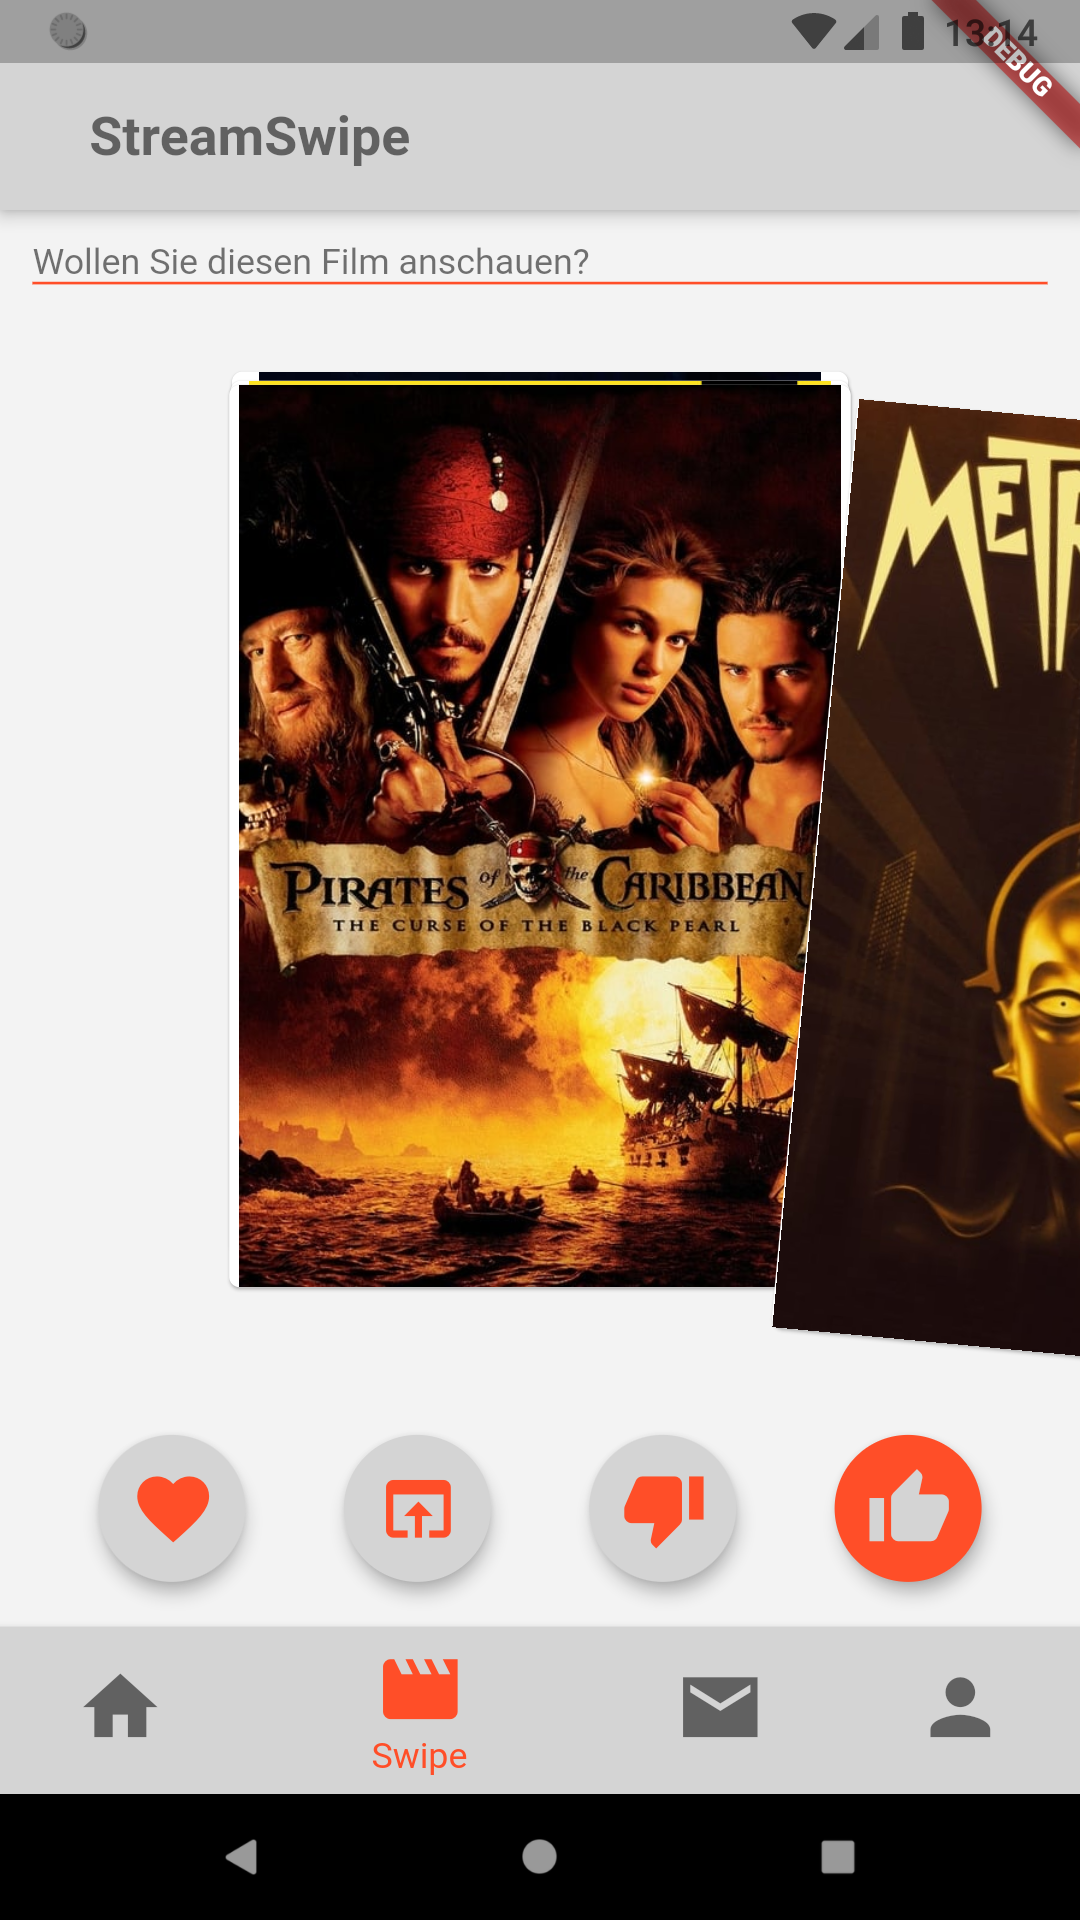
\includegraphics[scale=0.13]{Benutzeroberfläche/images/screenshot_swipescreen4.png}
	\caption{}
	\label{fig:swipescreen_d}
	\end{subfigure}
	\begin{subfigure}{0.33\textwidth}
	\centering
	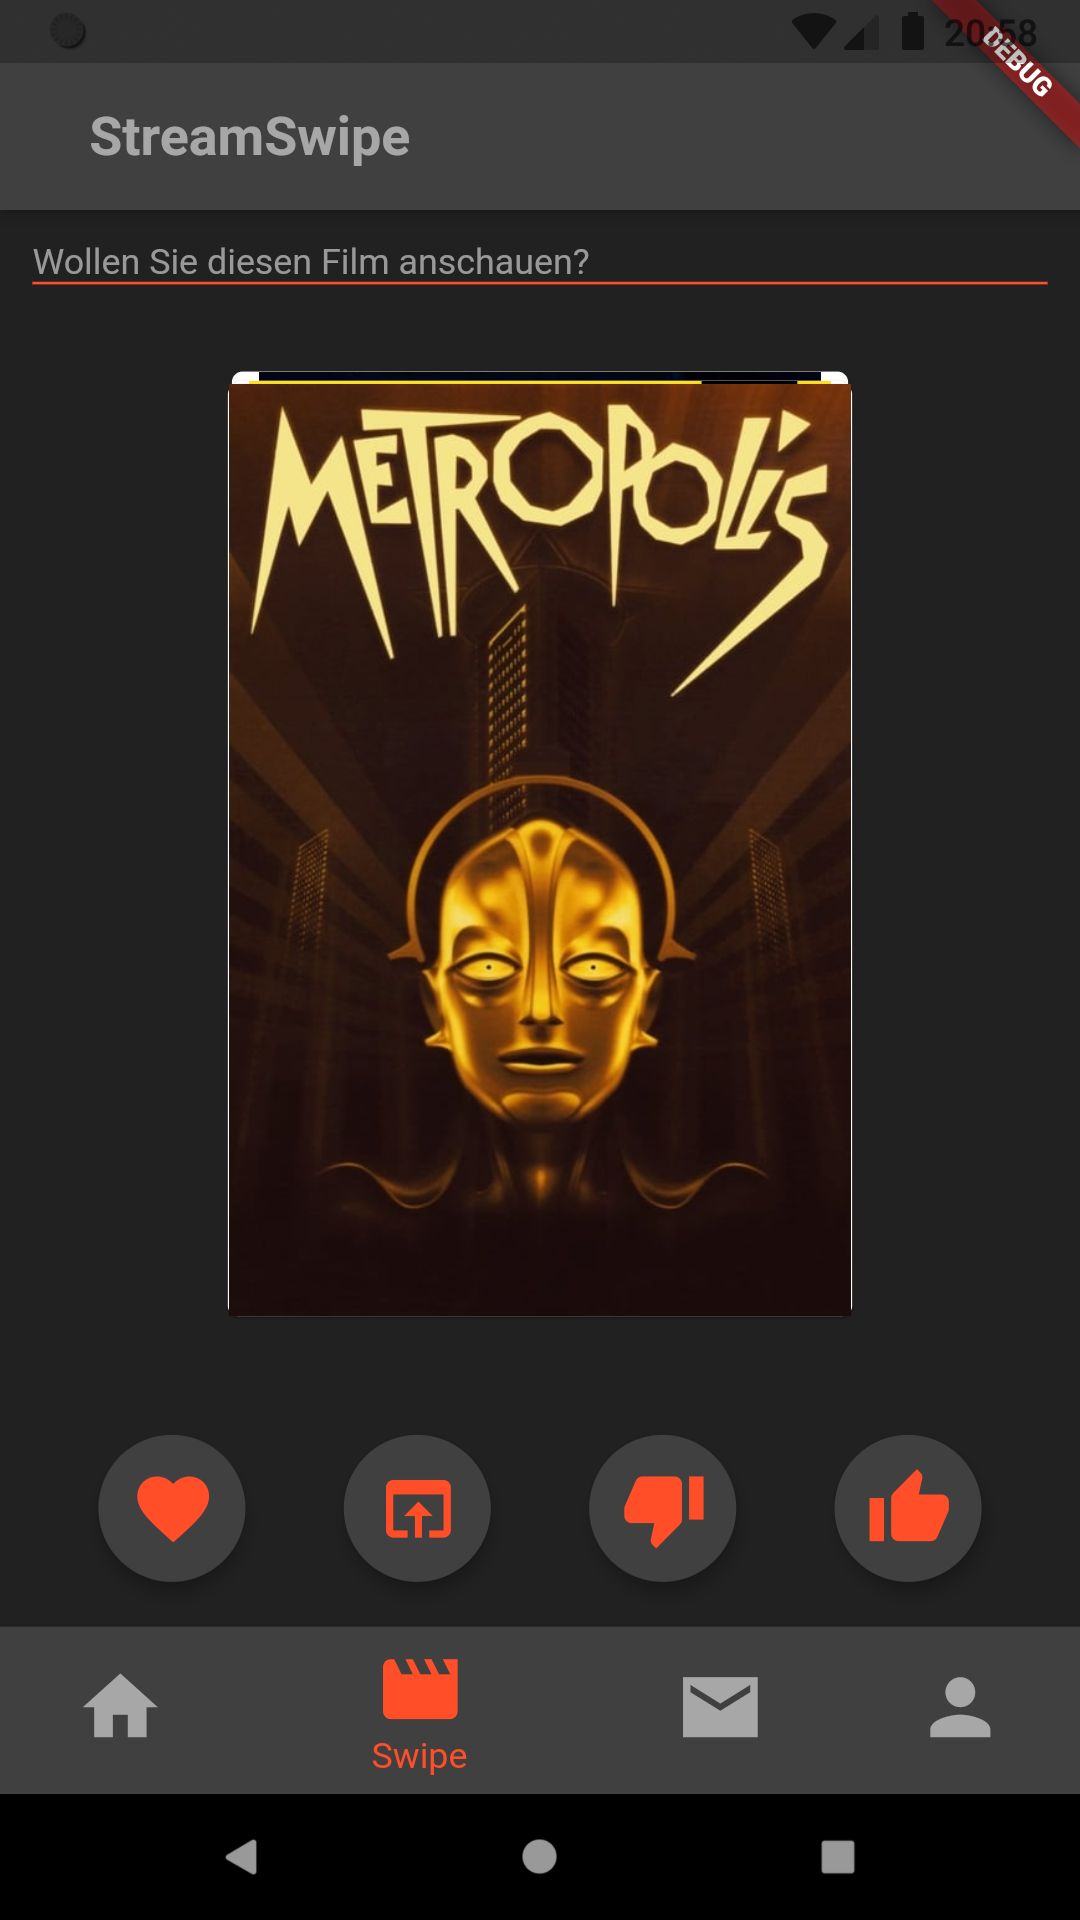
\includegraphics[scale=0.13]{Benutzeroberfläche/images/screenshot_darkmode_2.png}
	\caption{}
	\label{fig:swipescreen_e}
	\end{subfigure}
\caption{Darstellungen und Funktionen des Swipe-Screens mit (a) der Standarddarstellung, (b) weiteren Filminformationen, (c) einer Animation beim Drücken einer der Indikatoren und (d) der Swipe-Animation.  Hat der User in den Systemeinstellungen den dunklen Modus aktiviert, so wird (e) der Swipe-Screen wie alle anderen Screens angepasst.}
\label{fig:swipescreen_alle}
\end{figure}
\clearpage
\subsubsection{Chat}
\label{sec:UI-Chat}
Die Chatseite ist in eine Liste aus aktiven Chats und eine Warteliste aufgeteilt, siehe \ref{fig:chat_a} und \ref{fig:chat_b}. Um zwischen diesen beiden Listen zu wechseln werden Tabs eingesetzt, wie sie aus Windowsanwendungen bekannt sind. Zwischen diesen Tabs kann entweder gewechselt werden, indem ein anderes Tabfenster angetippt wird, oder der gesamte Bildschirm mit einer Geste zur Seite gewischt wird. Bei jedem Element der Chatliste ist der jeweilige Benutzername und die neueste Nachricht zu sehen, dazu wird falls vorhanden entweder ein Profilbild oder eine einfarbige Fläche mit dem Anfangsbuchstaben des Namens angezeigt. Chat Requests können jeweils durch das Schieben nach links angenommen oder nach rechts ablehnt werden, wie in den Abbildungen \ref{fig:chat_c}, bzw. \ref{fig:chat_d} zu sehen ist. Diese Mechanik wird häufig in Email-Apps zum Löschen oder Verschieben der Mails benutzt.\\ %TODO (screenshots normal, annehmen und ablehnen)
Durch Antippen eines Matches, öffnet sich der Chatverlauf, welcher in Abbildung \ref{fig:chat_e} zu sehen ist. Die Anordnung der Nachrichten innerhalb des Chatverlaufs ist wie aus anderen Messenger bereits bekannt, aber in den Stilfarben von StreamSwipe. Am oberen Bildschirmrand wird der Profilname des Matches angezeigt und rechts davon befindet sich der Button zu dessen Profilseite, auf der genauere Details über diese Person zu finden sind. Die Profilseiten werden in Kapitel \ref{sec:benutzerprofil} genauer vorgestellt. \\
Dem User wird durch das ihm bereits vorgestellte Design und der ausschließlichen Nutzung von bekannter Mechanik ein vertrautes Umfeld geboten. Wie auf jedem Screen passt sich auch hier das Farbschema automatisch an, falls in den Systemeinstellungen des Smartphones das dunkle Design gewählt wurde, wie beispielsweise in Abbildung \ref{fig:chat_f} dargestellt. Neben der Benutzerfreundlichkeit wird auch die Barrierefreiheit beachtet, indem alle Elemente, die nicht bereits aus einem Text bestehen, mit Semantiken ausgestattet werden. Zusätzlich werden keine feinmotorischen Bewegungen zur Navigation durch die Bildschirme benötigt. Bis auf die Eingabe über die Tastatur kann alles über große Flächen oder Wischmechaniken bedient werden. Im Chatverlauf wir die Standardtastatur des Systems verwendet, mit der der Benutzer bereits vertraut ist. 


\begin{figure}[H]
	\begin{subfigure}{0.33\textwidth}
	\centering
	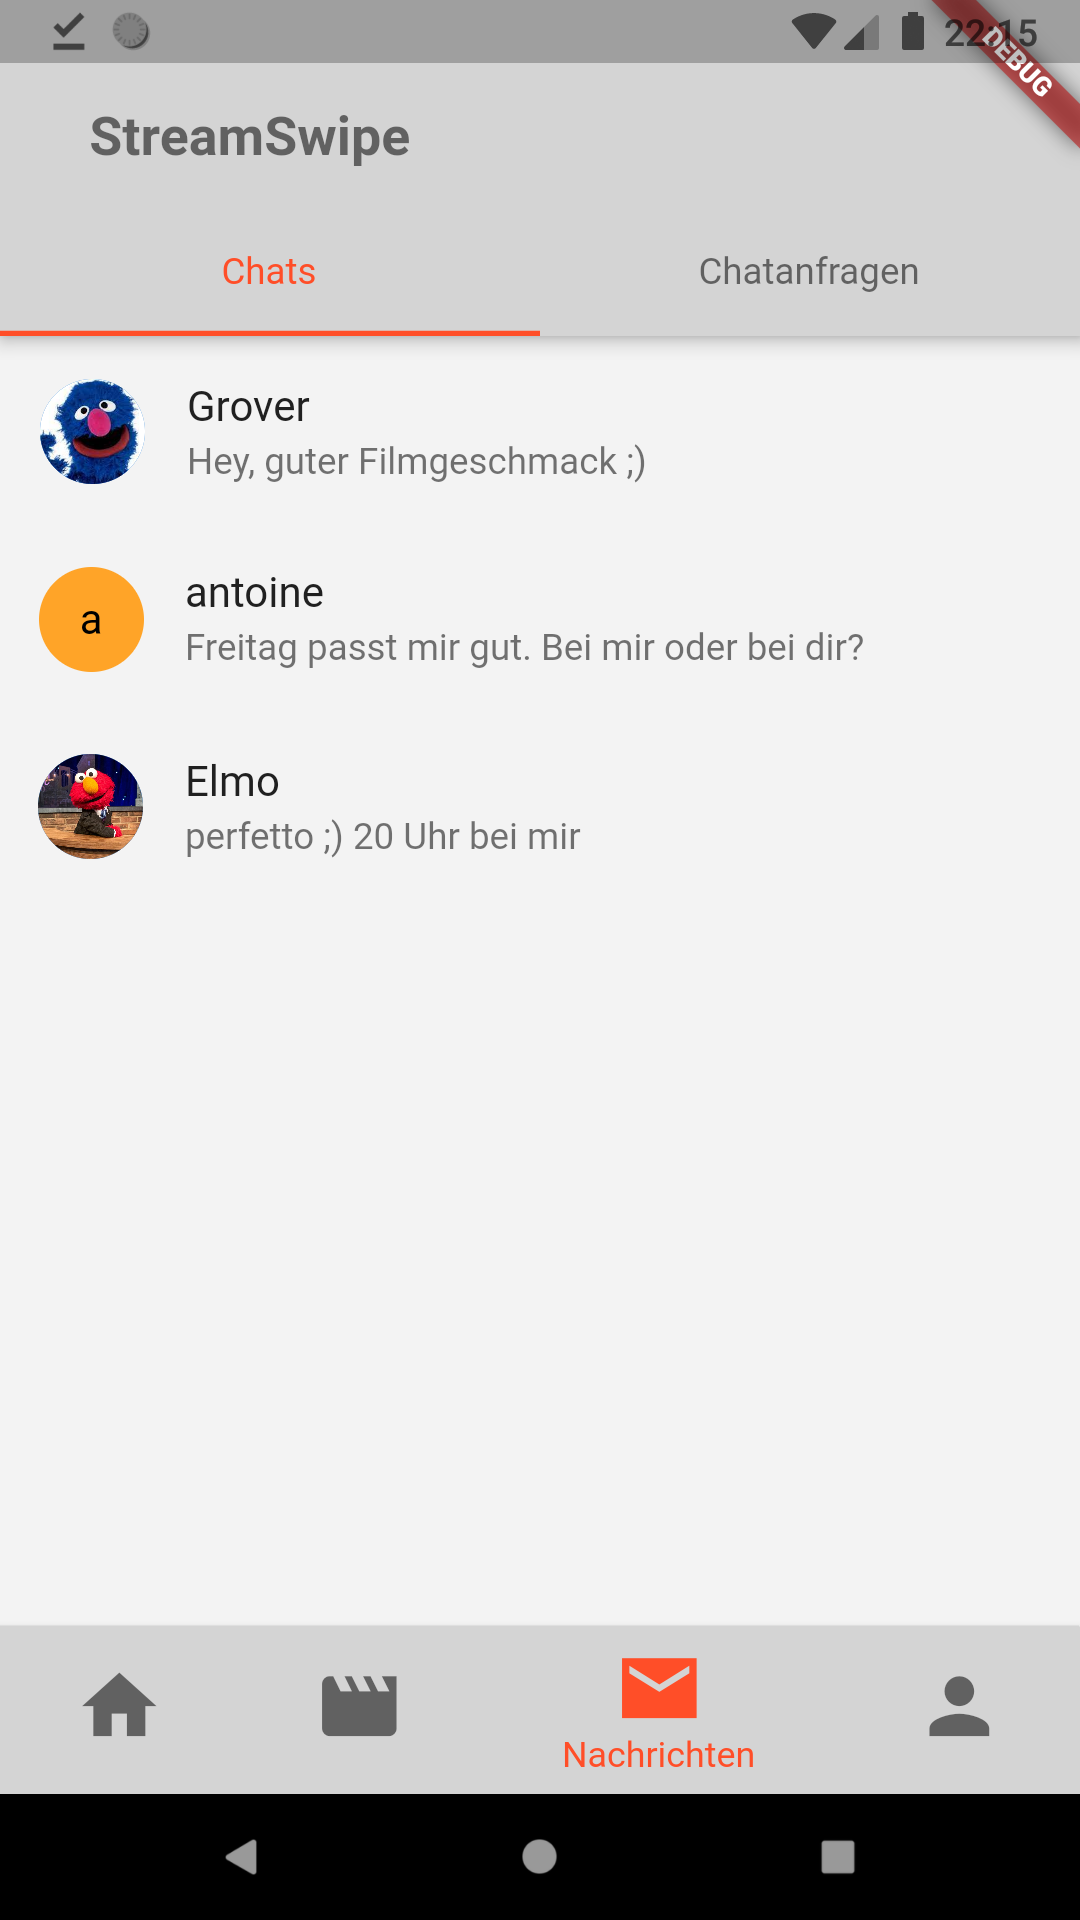
\includegraphics[scale=0.1742]{Benutzeroberfläche/images/screenshot_chat_1.png}
	\caption{}
	\label{fig:chat_a}
	\end{subfigure}
	\begin{subfigure}{0.33\textwidth}
	\centering
	
\includegraphics[scale=0.1742]{Benutzeroberfläche/images/screenshot_chat_2.png}
	\caption{}
	\label{fig:chat_b}
	\end{subfigure}
	\begin{subfigure}{0.33\textwidth}
	\centering
	\includegraphics[scale=0.1742]{Benutzeroberfläche/images/screenshot_chat_3.png}
	\caption{}
	\label{fig:chat_c}
	\end{subfigure}\\ \vspace{1cm}	
	
	\begin{subfigure}{0.33\textwidth}
	\centering
	\includegraphics[scale=0.1741]{Benutzeroberfläche/images/screenshot_chat_4.png}
	\caption{}
	\label{fig:chat_d}
	\end{subfigure}
	\begin{subfigure}{0.33\textwidth}
	\centering
	\includegraphics[scale=0.13]{Benutzeroberfläche/images/screenshot_chat_5.png}
	\caption{}
	\label{fig:chat_e}
	\end{subfigure}
	\begin{subfigure}{0.33\textwidth}
	\centering
	\includegraphics[scale=0.13]{Benutzeroberfläche/images/screenshot_darkmode_4.png}
	\caption{}
	\label{fig:chat_f}
	\end{subfigure}
\caption[Screenshots der Chat-Seiten]{Darstellungen und Funktionen der Chat-Screens mit (a) den aktiven Chats, (b) den Chats auf der Warteliste, (c) und (d) angenommene, bzw. abgelehnten Chats auf der Warteliste, sowie (e) einem Chatverlauf im hellen und (f) in dunklen Modus.}
\label{fig:chat_alle}
\end{figure}

\subsubsection{Benutzerprofil}
\label{sec:benutzerprofil}

Auf der Profilseite werden ein Profilbild, ein Hintergrundbild und für das Matching relevante persönliche Informationen dargestellt. Es gibt eine Version, die nur von anderen Nutzern sichtbar ist, mit denen ein Match stattgefunden hat, und eine Version, die über die Bottom-Navigation-Bar erreichbar werden kann. Die Letztere wird in Abbildung \ref{fig:profilseite_alle} dargestellt und unterscheidet sich von der Version für andere Nutzer darin, dass Profil- und Hintergrundbild bearbeitet werden können.\\
Das Farbschema und das Design wurden an die bisherigen Seiten angepasst. Um die Oberfläche simpel und selbsterklärend zu halten, wird jede dargestellte Information mit einem passenden Icon und einem Hinweis versehen (siehe Abbildung \ref{fig:profilseite_a}). Die Icons zum Bearbeiten der Bilder sind, wie auch in vielen anderen Apps, platziert und designt. Sie öffnen die systemeigene Bildergalerie des Smartphones um den Nutzer aus einem bekannten Umfeld Bilder auswählen lassen zu können.\\
Beim initialen Öffnen einer Profilseite sollen Namen, Profilbild und ein Hintergrundbild ins Auge springen. Sie stellen die ersten Informationen dar, die dem Betrachter wichtig sind, weshalb sie wie in Abbildung \ref{fig:profilseite_a} deutlich sichtbar ist  beim Öffnen mehr als die Hälfte des Bildschirms einnehmen. Anschließend wird der Fokus auf detailliertere Informationen gerichtet. Auf der Profilseite von StreamSwipe wird hierfür heruntergescrollt um den Block mit den Profildaten sehen zu können. Bei dieser Aktion blendet eine Animation das Profilbild aus und verschmälert das Hintergrundbild. Der Benutzername wird ebenfalls aus dem Fokus gezogen, bleibt aber wie in Abbildung \ref{fig:profilseite_b} zu sehen mit dem verbleibenden Hintergrundbildausschnitt erhalten. Dies hilft dem Betrachter unterbewusst bei dem Fokuswechsel und schafft ein modernes, responsives Feedback bei der User Experience.\\
Um das durchgängig schlichte Design der App zu erhalten ist der Zugang zu den Einstellungen ausschließlich auf der Profilseite zu finden. Hierfür ist im rechten oberen Bildschirmbereich das repräsentative Icon. Der hierdurch erreichbare Bildschirm (Abbildung \ref{fig:profilseite_c}) ist gleich aufgebaut wie die Informationeneingabe nachdem ein neuer Account erstellt wurde (Abbildungen \ref{fig:login_c} und \ref{fig:login_d}). Die dort angegebenen Informationen können hier wieder angepasst werden. %TODO Referenz auf account erstellen bild


\begin{figure}[tbt]
	\begin{subfigure}{0.33\textwidth}
	\centering
	\includegraphics[scale=0.13]{Benutzeroberfläche/images/screenshot_profilseite_1.png}
	\caption{}
	\label{fig:profilseite_a}
	\end{subfigure}
	\begin{subfigure}{0.33\textwidth}
	\centering
	\includegraphics[scale=0.13]{Benutzeroberfläche/images/screenshot_profilseite_2.png}
	\caption{}
	\label{fig:profilseite_b}
	\end{subfigure}
	\begin{subfigure}{0.33\textwidth}
	\centering
	\includegraphics[scale=0.13]{Benutzeroberfläche/images/screenshot_profilseite_3}
	\caption{}
	\label{fig:profilseite_c}
	\end{subfigure}
\caption[Screenshots der Profilseite]{Profilseite wie sie für den Nutzer selbst angezeigt wird (a) im normalen Zustand und (b) nach vollständigem Einklappen des Profilkopfes durch eine Animation während dem Herunterscrollen. Mit den von hier aus erreichbaren Einstellungen (c) können die anfänglich gegebenen Profilangaben abgepasst werden.}
\label{fig:profilseite_alle}
\end{figure}




\clearpage
\section{Probleme}
\label{sec:probleme}
In der Planungsphase eines Projektes werden oft große Meilensteine gesetzt. Sobald das Thema bekannt ist, werden durch Brainstorming und andere Methoden der Ideenfindung in kurzer Zeit viele Ziele gesteckt und ein in der Theorie fertiges Projekt ausgearbeitet. Eine Begrenzung wird nur durch die Fantasie der Beteiligten gezogen, die jedoch später in der Umsetzung schnell erreicht wird. Aber auch bei realistischen Zielen wird oft eine sehr spezielle Vorstellung angestrebt, die mit den gegebenen oder gewählten Mittel nur bedingt umsetzbar ist. Neben den Arbeitsmitteln zählen aber auch Zeit und Geld zu den einschränkenden Ressourcen.\\

\noindent
Wie unzählige Projekte vor uns, konnten wir ebenfalls nicht alle zu Beginn gesteckten Ziele zu unserer vollsten Zufriedenheit abschließen. Auch wenn alle grundlegend wichtigen Kriterien erfüllt sind und funktionieren, gibt es auch nicht erreichte Ziele. Diese bestehen aus erkennbaren und nicht erkennbaren Schwächen in der App. Ersteres sind Unsauberkeiten, die der User bei der Benutzung in manchen Situationen bemerken kann. Hierzu zählen beispielsweise Designfehler, die bei der Programmierung nicht erkannt wurden. Nicht erkennbare Schwächen sind Ideen und Ziele, die im vorgegebenen Rahmen nicht mehr eingebaut werden konnten. Diese fallen nur dem Programmierer auf. In unserem Fall ist das Fehlen mancher Funktonen hauptsächlich auf Zeitmangel zurückzuführen. Bei einem zeitlich begrenzten Bearbeitungsrahmen, während dem noch einige andere Projekte, Vorlesungen, Prüfungen und eine Arbeitsstelle in Vollzeit belegt werden, können nicht alle beabsichtigten Features eingebaut werden. Alle geplanten Erweiterungen wurden jedoch bereits durchdacht und werden nach Abgabe der schriftlichen Arbeit implementiert, aber hierzu mehr in Kapitel \ref{sec:fazit}.\\

\noindent
Da StreamSwipe in Deutschland entwickelt und programmiert wurde, liegt es nahe Deutsch als In-App-Sprache zu verwenden. Außer den auf den Oberflächen angezeigten Texten müssen auch Fehlermeldungen, Semantiken und Autovervollständigungen angepasst werden. Wie auf den Screenshots im ganzen Kapitel \ref{sec:UI-alle} zu sehen ist, wird dies in der App konsequent durchgesetzt. Die Filmdatenbank, aus der die dargestellten Informationen erhalten werden, liefert diese jedoch nur auf Englisch, was an der Handlungsangabe in Abbildung  \ref{fig:swipescreen_b} zu sehen ist. Alle Datenbanken, die in Kapitel  \ref{sec:filmdatenbank} betrachtet werden, bieten ihre Informationen nur in einer Sprache an. Eine Lösung dieses Problems wird in Kapitel \ref{sec:ausblick} beschrieben.\\

\noindent
Bei einer sauberen Implementierung werden die Elemente auf den Bildschirmen in Abhängigkeit der Gesamtgröße des Screens angeordnet, sodass sie sich auf unterschiedlichen Geräten entsprechend anordnen und ihre Größe anpassen können. Man spricht hierbei von responsivem Design, auf welches bei StreamSwipe ebenfalls Wert gelegt wurde. Je nach Verhältnis von Breite und Höhe der Bildschirmgrößen unterschiedlicher Geräte können so in Grenzfällen jedoch ungewollte Verzerrungen auftreten. Das Aussehen einer Benutzeroberfläche kann außerdem auch von dem verwendeten Betriebssystem abhängen, da unterschiedliche Generationen unterschiedliche Standards verwenden. Durch die begrenzte Entwicklungszeit  und den limitierten Zugang zu Ressourcen konnte die App nur auf einer kleinen Anzahl von  Endgeräten getestet und angepasst werden. Es kann somit leider keine Garantie für eine saubere Darstellung auf älteren Geräten gegeben werden. Längere Testphasen könnten dieses Problem minimieren, jedoch ist der Markt von Smartphones mittlerweile so unübersichtlich groß, dass es nahezu unmöglich ist jede Variation zu testen.\\

\noindent
Das wahrscheinlich größte Manko ist das Ausbleiben der Veröffentlichung der App am Abgabetermin der schriftlichen Arbeit. Ursprünglich geplant war eine Veröffentlichung in Google Play für Androidgeräte und im App Store für iPhones, weshalb wie in Kapitel \ref{sec:flutter} beschrieben Flutter als Framework verwendet wurde. Bei einer Veröffentlichung in Google Play wird die App vor Release einer umfangreichen Überprüfung unterzogen, was voraussichtlich eine Woche und in manchen Fällen auch länger dauern kann \cite{playstore_release}. Außerdem muss das vom Webserver benutzte Sicherheitszertifikat zur Kommunikation über HTTPS von einer offiziellen Zertifizierungsstelle signiert werden. Wie bereits in Kapitel \ref{sec:SichereKommunikation} angesprochen, benutzen wir ein selbstsigniertes Zertifikat. Zu den Kosten dieser Zertifizierung wird noch eine Mitgliedschaft als Google Play Developer von einmalig \$\,25 benötigt \cite{kostenPlayStoreDeveloper}. Für eine  Veröffentlichung im App Store ist eine Mitgliedschaft im Apple Developer Programm notwendig, die jährlich \$\,99 kostet \cite{appstore_release}. Diese Investitionen werden erst sinnvoll, wenn ein Monetarisierungsplan der App ausgearbeitet wurde.. \\

\noindent
Wie in Kapitel \ref{sec:komponenten} bereits erwähnt, werden die Verteilung der Film-IDs und die Auswertung der Filmbewertungen auf einem Server ausgeführt. Dieser Server besteht zur Zeit aus einem Raspberry Pi. Für den Gebrauch während der Entwicklungsphase ist die somit erreichte Rechenkapazität völlig ausreichend, da nur maximal drei Personen gleichzeitig darauf zugegriffen haben. Sollte die App jedoch veröffentlicht werden, werden die Nutzerzahlen unvorhersehbar ansteigen, sodass nicht vorausgesagt werden kann, ab wann der Server in diesem Aufbau überlastet sein wird. Um den Benutzern eine positive User Experience bieten zu können und eventuelle Hardwareschäden an dem Raspberry Pi zu vermeiden, muss mit der Veröffentlichung der App gewartet werden bis eine leistungsstärkere Lösung gefunden wurde.


\clearpage
\section{Anwendbarkeit}
\label{sec:anwendbarkeit}
Die theoretische Planung einer App weicht oft von der späteren praktischen Anwendung ab. Dies kann unterschiedliche Gründe haben, die hier zum Teil beleuchtet werden sollen.\\

\noindent
Bei der Entwicklung einer App werden Funktionen für gutmütige Benutzer implementiert. Auch wenn dieses Vorgehen unbewusst auftritt, ändert es nichts daran, dass es sich hierbei um eine naive Herangehensweise handelt. Die eingebauten Funktionen werden in der Regel so ausgelegt, dass sie bei sachgemäßer Benutzung problemlos funktionieren. Wie sie jedoch  in der Praxis angewendet werden, wird hierbei oft nicht bedacht. Die unsachgemäße Benutzung muss nicht mutwillig durch die Nutzer geschehen, kann jedoch durch einfache Bedienfehler Probleme verursachen. Beim Programmieren der Features sollte deshalb auf verschiedene Problemherde eingegangen werden.\\

\noindent
\hangindent1cm
\textbf{Falscheingaben:} Hierzu zählen freiwillige und unfreiwillige Falscheingaben. Unfreiwillige Angaben sind beispielsweise Tippfehler oder falsche Filmpräferenzierung. Ersteres wird teilweise bei der Eingabe überprüft, wie etwa die E-Mail-Adresse, die eine bestimmte Form aufweisen muss, und andere Angaben können später in den Einstellungen korrigiert werden. Falsche Filmbewertungen können in unserem Fall jedoch nicht rückgängig gemacht werden, sollten aber auf zwischenmenschlichem Wege nach einem Matching vom Nutzer gelöst werden können.\\
Unter freiwilligen Falscheingaben versteht man falsche Datenangaben, was bei einem falschen Namen zur Anonymisierung führt. Das Matchingverfahren wird über den angegebenen Wohnort gemacht, sodass durch einen Wohnortwechsel der potentielle Personenkreis geändert wird. Da StreamSwipe von einer hohen Nutzerdichte pro Wohnort profitiert, wirkt sich dies negativ auf den vom Nutzer verlassenen Wohnort aus. Es ist möglich den Nutzerstandort per GPS auszulesen, jedoch können so Nutzer in einem schwach besiedelten Gebiet nicht in die nächstgrößere Stadt wechseln und die Filterung bei der Matchberechnung wäre dann wesentlich feinmaschiger und rechenaufwändiger.\\

\noindent
\hangindent1cm
\textbf{Schließen\,der\,App:} Falls die App beispielsweise während einer Datenangaben geschlossen wird, können unerwartete Fehler auftreten. Die Auswirkungen  variieren,  abhängig davon, an welchem Zeitpunkt die App geschlossen wird. Im schlimmsten Fall sind die Benutzerdaten anschließend beschädigt und verursachen einen Absturz der App beim nächsten Start.\\

\noindent
\hangindent1cm
\textbf{Funktionenmissbrauch:} Ist der genaue Vorgang hinter einer Funktion bekannt, kann diese schnell missbraucht werden. Bei dem Bewertungsverfahren von StreamSwipe wird über eine große Anzahl von Filmen ein Präferenzprofil erstellt und eine Übereinstimmung mit anderen Profilen über einem gewissen Prozentsatz gesucht. Wird jedoch ein Film mit \glqq Superlike\grqq \, bewertet, so matcht das System alle Nutzer, die diesen Film ebenfalls mit \glqq Superlike\grqq \, bewertet haben. Außerdem fließt die Bewertung \glqq Superlike\grqq \, ebenfalls in die Erstellung des Präferenzprofils. Wenn also ein Nutzer ausschließlich Filme superliket, unabhängig ob ihm der Film gefällt, kann er eine sehr hohe Anzahl an Matches erreichen. Jedoch wird durch diese Art des Matchings nicht das ursprünglich geplante Ziel aus Kapitel \ref{sec:einleitung} erreicht und Nutzer, die die App ernsthaft für einen gelungenen Filmeabend benutzen, könnten sich betrogen fühlen und die App wieder deinstallieren.\\
Es ist bereits geplant die Anzahl der gespeicherten Superlikes pro Nutzer zu begrenzen, sodass ab einer gewissen Anzahl alte Superlikes gelöscht werden wenn Neue hinzukommen.  Nur die aktuell gespeicherten Superlikes werden auch zum Matching verwendet. Die Implementierung dieses Updates kann auch nach Abgabe dieser Dokumentation geschehen, da es in der Regel selbst nach der Veröffentlichung einer App eine Weile dauert bis solche Schlupflöcher gefunden werden.\\

\noindent
Die Praxis zeigt jedoch, dass auch bei guten anfänglichen Überlegungen nicht alle Probleme beseitigt werden können, da diese teilweise zu vielschichtig sind oder sich mit anderen gewollten Features überschneiden. Trotz umfangreicher Maßnahmenergreifung kann nie vorausgesagt werden wie sich etwas entwickelt. Uber wurde beispielsweise ursprünglich als Limousinenservice gegründet und ist heute eines der größten Taxiunternehmen weltweit. Deshalb sollte bei der Planung bedacht werden was die Nutzer eigentlich wollen und welche Funktionen in der Praxis wirklich genutzt werden. Bei einer Dating-App geht es darum möglichst einfach mit anderen Personen Kontakt aufzunehmen.  Das Swipen von Filmpostern sollte in den meisten Fällen kein Hindernis darstellen. Ein großer Prozentsatz der Nutzer einer Dating-App verfolgt bei der Benutzung ein sehr spezielles Ziel, auf das bei StreamSwipe keinen Fokus gelegt wurde. Jedoch existiert hierbei bereits zu Beginn des Matches zwischen den beteiligten Personen ein gemeinsames Thema und ein Filmabend ist für diese Absicht wahrscheinlich zielführender als manch anderer Vorwand. \\
Sicher lockt StreamSwipe auch Personen an, die gerne  neue Filme und Personen mit ähnlichem Geschmack kennenlernen würden. Hierfür bietet sich StreamSwipe optimal an, sobald Filmempfehlungen implementiert werden, mehr dazu in Kapitel \ref{sec:ausblick}.\\

\noindent
Ebenso relevant wie die bestehenden Bedürfnisse der Nutzer, sind die bisherigen Lösungen, die der Markt bietet. Hierzu müssen alle Apps betrachtet werden, die die selben Funktionen wie StreamSwipe anbieten. Schränkt man die Funktionen auf das wesentliche ein, sodass der Fokus auf dem Bewerten von Filmen ist wodurch neue Leute kennengelernt werden, ist der Markt noch absolut frei. Keine andere App bietet diese Funktionen an, jedoch existieren ähnliche Konzepte, die aber alle für Einzelpersonen oder bestehende Gruppen Filmvorschläge auf Basis der bewerteten Filme bieten. Das Matching mit neuen Leuten ist bisher noch nicht vertreten, was die perfekte Basis für einen Marktstart bietet.


\clearpage
\section{Ausblick}
\label{sec:ausblick}
Die Entwicklung und Programmierung der App war ein wichtiger und großer Schritt, jedoch ist er nicht der Letzte. Für die nun kommende Zeit stehen bereits einige Aufgaben fest um das Projekt StreamSwipe aufrechtzuerhalten.\\
Wie bereits in Kapitel \ref{sec:probleme} erwähnt, konnten nicht alle gewünschten Features eingebaut werden. Sie waren während der Entwicklungsphase entweder von zu geringer Priorität, oder sind erst im späteren Stadium aufgekommen. Beispielsweise werden die Filmdaten bisher nur auf Englisch erhalten. In einer sonst deutschsprachigen App ist diese Umstellung jedoch schon in Planung. Es existieren deutsche Filmdatenbanken wie beispielsweise OFDb, aus denen die übersetzten Daten erhalten werden können. Diese ist leider nicht so umfangreich wie die bisher genutzte Datenbank, sodass dann von beiden parallel Daten erhalten und abgeglichen werden um die User Experience nicht zu mindern.  In diesem Zuge ist auch eine optionale In-App-Sprache geplant, die der Benutzer auswählen kann, da nun die Informationen auf Deutsch und auf Englisch vorliegen. Um die Sprache der App ändern zu können, müssen alle Textelemente durch Variablen ersetzt werden, die in einer zentralen Tabelle beschrieben werden. Für eine andere Sprache werden diese Variablen dann mit den übersetzten Formulierungen überschrieben. Ist die App angepasst und der Datenfluss der beiden Datenbanken synchronisiert, können auch mit weniger Aufwand auch andere Sprachen in das System aufgenommen werden.\\

\noindent
Ein Update, bei dem Filmempfehlungen eingeführt werden, ist bereits geplant. Hierbei werden auf Basis der berechneten Filmpräferenz und den Überschneidungen innerhalb eines Matches eine Liste mit Filmvorschlägen generiert. Dieses Feature ist von großer Bedeutung wenn man bedenkt wie viel Zeit in die Suche eines geeigneten Filmes gesteckt wird.\\
Auch das Ressourcenproblem des Servers kann in absehbarer Zeit behoben werden. Da die Skripte auf dem Raspberry Pi bereits geschrieben sind, ist lediglich eine leistungsstärkere Hardware nötig um einen stabilen Server zu realisieren. Solange die Benutzerzahlen und somit auch die benötigte Leistung überwacht werden, kann frühzeitig ohne Datenverlust oder Performanceeinbußen auf ein größeres System umgestellt werden.\\
Ist die App dann für die Öffentlichkeit zugänglich, lohnt es sich ein Feedbacksystem zu nutzen, durch welches die Nutzer Lob und Kritik äußern können. Oft treten kleine Bugs nur in sehr speziellen Situationen auf, die während der Testphase nicht bedacht oder nicht realisiert werden. \\

\noindent
Werbung spielt einen entscheidenden Faktor in der Kundengewinnung. Mithilfe gezielter Produktplatzierungen, möglichst großflächiger Marketingstrategien und zufriedenen Bestandskunden kann innerhalb von wenigen Wochen ein beachtlicher Kundenstamm aufgebaut werden. Timing ist in diesem Fall sehr wichtig, da die angeworbenen Kunden möglichst gleichzeitig mit der App bekannt gemacht werden sollten. StreamSwipe basiert auf einem möglichst flächendeckenden Kundenkreis, da nur lokal gematcht wird und ein Nutzer ohne Matches nicht lange gehalten werden kann. Entsprechend ergibt es Sinn gezielte Werbung in einer lokalen Umgebung einzusetzen  und lieber eine hohe Benutzerdichte, als eine große Reichweite aufzubauen. Wird die App in diesem Umfeld genutzt und somit Matches generiert, verbreitet sie sich automatisch auch in umliegende Städte und beginnt so zu wachsen. Mit dem Benutzerradius sollte auch der Radius der geschalteten Werbung sukzessiv vergrößert werden.


\clearpage
\section{Fazit}
\label{sec:fazit}
-


- App ist fast fertig und funktioniert
- ziele der Einleitung erreicht??? eher nicht, also erst ab Markteinführung kann man darüber wirklich eine Aussage machen.


Verbesserungswürdig, aber es ist eine gelungene Option neue Menschen und neue Filme kennenzulernen.


- welche ziele haben wir erreicht?
- gutes/schlechtes
- nicht perfekt (kleine bugs), aber wann ist man wirklich fertig??? Nichtmal Gott ist mit seiner Schöpfung wirklich fertig


\clearpage
\appendix
\section{Verfasser einzelner Abschnitte}
\newcolumntype{L}[1]{>{\raggedright\let\newline\\\arraybackslash\hspace{0pt}}m{#1}}
\newcolumntype{C}[1]{>{\centering\let\newline\\\arraybackslash\hspace{0pt}}m{#1}}

\begin{table}[H]
	\centering
	\begin{tabular}{L{1cm} L{6.5cm} C{7.5cm}}
		\toprule
		\multicolumn{2}{l}{\textbf{Kapitel / Abschnitt}}                               							& \textbf{Verfasser}\\ 
		\midrule
		\multicolumn{2}{l}{1. Einleitung}                                             							& Vincent Schreck\\ 
		 	& 1.1 Motivation                              														& Vincent Schreck\\
			& 1.2 Methode                                    													& Vincent Schreck\\ 
		\midrule
		\multicolumn{2}{l}{2. Theoretische Grundlagen}                        									& Leon Gieringer \& Robin Meckler\\
		 	& 2.1 Netzwerkprotokolle                                                  							& Robin Meckler\\
			& 2.2 JavaScript                                     												& Robin Meckler\\
			& 3.3 NodeJS                                                              							& Robin Meckler\\
			& 2.4 Representational State Transfer - Application Programming Interface							& Robin Meckler\\
			& 2.5 NoSQL-Datenbank                                                     							& Robin Meckler\\ 
		\midrule
			& 2.6 Firebase                                       												& Leon Gieringer\\
			& 2.7 Anwendungsentwicklung für mobile Endgeräte                          							& Leon Gieringer\\
			& 2.8 Frameworks zur mobile, plattformübergreifenden Entwicklung          							& Leon Gieringer\\
			& 2.9 Recommender Systems                                                 							& Leon Gieringer\\ 
		\midrule
		\multicolumn{2}{l}{3. Konzept}                                         									&  Vincent Schreck \\ 
		\midrule
		\multicolumn{2}{l}{4. Auswahl geeigneter Technologie}                                      		 		& Leon Gieringer \& Robin Meckler\\
			& 4.1 Anwendungsframework																			& Leon Gieringer \\
			& 4.2 Server                                         												& Robin Meckler \\
			& 4.3 Datenbank                                                           							& Robin Meckler \\
			& 4.4 Kommunikationsschnittstelle                    												& Robin Meckler \\ 
			& 4.5 Film-Datenbank                    															& \\ 
		\midrule
		\multicolumn{2}{l}{5. Backend-Implementierung}                                              			& Robin Meckler\\
			& 5.1 Server																						& Robin Meckler\\
			& 5.2 Datenbank                                                           							& Robin Meckler\\
		\midrule
		\multicolumn{2}{l}{6. Funktionen/Komponenten}                                               			& \\
			& 6.1 Swipe/Aussuchen/Voting                         												& \\
			& 6.2 Matches/Chat                                                        							& Leon Gieringer\\
			& 6.3 Filmvorschläge                                	 											& \\
			& 6.4 Gespeicherte Filme                                                  							& \\
			& 6.6 Barrierefreiheit			       																& Vincent Schreck\\ 
		\midrule
		\multicolumn{2}{l}{7. Benutzeroberfläche}                                                   			& Vincent Schreck\\
			& 7.1 Aspekte von Benutzeroberflächen                                    							& Vincent Schreck\\
			& 7.2 Oberflächen von StreamSwipe                                                             		& Vincent Schreck\\
		\midrule
		\multicolumn{2}{l}{9. Probleme}                                                            				& \\ 
		\midrule
		\multicolumn{2}{l}{10. Anwendbarkeit}                                  									& \\ 
		\midrule
		\multicolumn{2}{l}{11. Fazit}                                       									& \\
		\bottomrule
	\end{tabular}
\end{table}

\clearpage
\section{Sicherheitsregeln}
\begin{lstlisting}[caption=Sicherheitsregeln Firestore, label=lst:appendix_firestore_rules]
	rules_version = '2';
	service cloud.firestore {
		match /databases/{database}/documents {
			match /users/{user} {
				allow write: if isAuthenticated() && request.resource.id == request.auth.uid;
				allow read: if isAuthenticated() && userExists();
				match /tokens/{token} {
					allow read, write: if isAuthenticated() && user == request.auth.uid;
				}
				match /chatRooms/{chatroom} {
					allow read, write: if isAuthenticated() && user == request.auth.uid;
				}
				match /pendingChatRooms/{chatroom} {
					allow read: if isAuthenticated() && userExists();
					allow write: if isPartOfChat(request.resource.id, request.auth.uid) || user == request.auth.uid;
				}
			}
			match /unreadMessages/{unreadMessage} {
				allow read, write: if isAuthenticated() && userExists()
			}
			match /chatroom/{chatRoomId} {
				allow create: if isAuthenticated() && userExists();
				allow write: if isPartOfChat(chatRoomId, request.auth.uid);
				allow read: if isAuthenticated() && userExists();
				
				match /messages/{messageId} {
					allow write, read: if isAuthenticated()  && userExists() && isPartOfChat(chatRoomId, request.auth.uid);
				}
			}    
			/******* Hilfsfunktionen *******/
			// Ueberprueft, ob der Anfragende angemeldet ist
			function isAuthenticated() {
				return request.auth != null;
			}
			// Ueberprueft, ob der Nuter einen Eintrag in Firestore besitzt
			function userExists() {
				return exists(userRef(request.auth.uid));
			}
			// Ueberprueft, ob das Array "users" in einem Chatraum die UID des Anfragenden enthaelt
			function isPartOfChat(chatRoomId, userId) {
				return (get(chatroomRef(chatRoomId)).data.users[0] == userId)
				|| (get(chatroomRef(chatRoomId)).data.users[1] == userId)
			}
		
			/******* Hilfsreferenzen *******/
			function chatroomRef(id){
				return /databases/$(database)/documents/chatroom/$(id);
			}
			function userRef(id) {
				return /databases/$(database)/documents/users/$(id);
			}
		}
	}
\end{lstlisting}
\clearpage

%TODO Abkürzungsverzeichnis
\section*{Abkürzungsverzeichnis}

- ECMA European Computer Manufacturers Association

\newpage


\clearpage
\section*{Literaturverzeichnis}
\begin{itemize}
%
%
%   	Grundlagen
%			NetzwerkProtokolle
%
%

\bibitem[Prot1]{wikiNetzwerkprotokolle} Wikipedia. Netzwerkprotokolle, \url{https://de.wikipedia.org/wiki/Netzwerkprotokolle}, letzter Zugriff: 06.04.2021

\bibitem[Prot2]{wikiOsiModell}  Wikipedia. OSI-Modell. \url{https://de.wikipedia.org/wiki/OSI-Modell}, letzter Zugriff: 06.04.2021

\bibitem[Prot3]{wikiDodModell} Wikipedia. DoD-Schichtenmodell. \url{https://de.wikipedia.org/wiki/DoD-Schichtenmodell}. letzter Zugriff: 06.04.2021

\bibitem[Prot4]{ekOSI} Elektronik Kompendium. OSI-Schichtenmodell. \url{https://www.elektronik-kompendium.de/sites/kom/0301201.htm}, letzter Zugriff: 06. April 2021

%
%
%   	Grundlagen
%			JavaScript
%
%

\bibitem[JS1]{JS1} Saternos, Casimir (2014). Client-Server Web Apps with JavaScript and Java. O'Reilly Media. Seite 32f. ISBN 978-1449369330

\bibitem[JS2]{JS1.05} Philip Ackerman (2018). JavaScript Das umfassende Handbuch. Rheinwerk Computing. Pp 45. ISBN 978-3-8362-5696-4

\bibitem[JS3]{JS1.06} Ingo Pakalski, 15 Jahre WWW: Die Browserkriege - Golem.de. \url{http://www.golem.de/0805/59377.html}, letzter Zugriff: 03. April 2021

\bibitem[JS4]{JS1.07} Ben Ilegbodu, History of ECMAScript.
\url{https://www.benmvp.com/blog/learning-es6-history-of-ecmascript/}, letzter Zugriff: 03. April 2021

\bibitem[JS5]{JS1.08} ECMA International, ECMAScript®2020 Language Specification \url{https://www.ecma-international.org/publications-and-standards/standards/ecma-262/},letzter Zugriff: 03. April 2021

\bibitem[JS6]{JS1.09} Paul Krill, ECMAScript 2021 spec for JavaScript nears the finish line. \url{https://www.infoworld.com/article/3613948/ecmascript-2021-spec-for-javascript-nears-the-finish-line.html}, letzter Zugriff: 03. April 2021

\bibitem[JS7]{JS1.091} David Flanagan, JavaScript The Definitive Guide,  Seite 1, ISBN 858-1-1222-6666-3

\bibitem[JS8]{JS1.1} David Flanagan, JavaScript The Definitive Guide,  Seite 2, ISBN 858-1-1222-6666-3

\bibitem[JS9]{JS1.2} Wikipedia, JavaScript, \url{https://en.wikibooks.org/wiki/JavaScript/Relation_to_other_languages}, letzter Zugriff: 03. April 2021

\bibitem[JS10]{JS1.29} Programiz, JavaScript object properties, \url{https://www.programiz.com/javascript/object}, letzter Zugriff: 03. April 2021

\bibitem[JS11]{JS1.3} Dipl.-Ing. (FH) Stefan Luber, Stephan Augsten. \url{https://www.dev-insider.de/was-ist-javascript-a-586580/}, letzter Zugriff: 03. April 2021

\bibitem[JS12]{JS1.4} Philip Ackerman, JavaScript Das umfassende Handbuch (2018), Rheinwerk Computing, Seite 46ff, ISBN 978-3-8362-5696-4

%
%
%   	Grundlagen
%			NodeJS
%
%



\bibitem[Node1]{Node1.05} Basarat Ali Syed , Beginning Node.js 2014 Seite 23ff. ISBN 978-1-4842-0187-9

\bibitem[Node2]{Node1.1} StrongLoop, What Makes Node.js Faster Than Java? \url{http://strongloop.com/strongblog/node-js-is-faster-than-java/}, letzter Zugriff: 03. April 2021

\bibitem[Node3]{Node1.2} Philip Ackerman (2018). JavaScript Das umfassende Handbuch. Rheinwerk Computing. Seite 868ff. ISBN 978-3-8362-5696-4

\bibitem[Node4]{Node1.21} Node.js documentation. \url{https://nodejs.org/api/modules.html#modules_caching},letzter Zugriff: Stand 05. April 2021

\bibitem[Node5]{Node1.3} Wikipedia. NPM. \url{https://de.wikipedia.org/wiki/Npm_(Software)}, letzter Zugriff: 05. April 2021

\bibitem[Node6]{Node1.4} Ahmad Nassri, So long, and thanks for all the packages! \url{https://blog.npmjs.org/post/615388323067854848/so-long-and-thanks-for-all-the-packages.html}, letzter Zugriff: 03. April 2021

\bibitem[Node7]{Node1.5} Alexander Neuman, Node.js 0.6.3 integriert npm
\url{https://www.heise.de/developer/meldung/Node-js-0-6-3-integriert-npm-1386141.html},letzter Zugriff: 03. April 2021

\bibitem[Node8]{Node1.6} https://expressjs.com/de/, letzter Zugriff: Stand 04. April 2021

\bibitem[Node9]{Node1.8} \url{https://developer.mozilla.org/en-US/docs/Learn/Server-side/Express_Nodejs/Introduction}, letzter Zugriff: 04. April 2021

\bibitem[Node10]{Node1.9} Philip Ackerman (2018). JavaScript Das umfassende Handbuch. Rheinwerk Computing. Seite 895ff. ISBN 978-3-8362-5696-4

\bibitem[Node11]{Node2.0} Lee Brandt, Build and Understand Express Middleware through Examples \url{https://developer.okta.com/blog/2018/09/13/build-and-understand-express-middleware-through-examples}, letzter Zugriff: 04. April 2021

\bibitem[Node12]{Node2.1} Express, API-Dokumentation. \url{https://expressjs.com/de/api.html}, letzter Zugriff: Stand 05. April 2021

\bibitem[Node13]{Node2.15} Weiterleitung (Routing). \url{https://expressjs.com/de/guide/routing.html},letzter Zugriff: Stand 05. April 2021

\bibitem[Node14]{Node2.5} Binariks, Express.js Mobile App Development: Pros and Cons for Developers. \url{https://binariks.com/blog/tools/express-js-mobile-app-development-pros-cons-developers/}, letzter Zugriff: 05. April 2021

\bibitem[Node15]{Node2.55} Basarat Ali Syed, Beginning Node.js, Seite 275, ISBN 978-1-4842-0187-9

\bibitem[Node16]{Node2.56} U. Störl, T. Hauf, M. Klettke and S. Scherzinger, "Schemaless nosql data stores—Object-NoSQL mappers to the rescue?", Proc. Datenbanksyst. Bus. Technologie Web (BTW), Seiten 579-599


\bibitem[Node17]{Node2.6} Simon Holmes. Mongoose for Application Development. Seite 124f. ISBN 978-1782168195

\bibitem[Node18]{Node3.2} Tim Ambler, Nicholas Cloud. JavaScript Frameworks for Modern Web Dev. Seite 321. ISBN 978-1-4842-0663-8


%
%
%   	Grundlagen
%			NoSQL
%
%

\bibitem[DB1]{DB1} Andreas Meier, Grundlagen, Systeme und Nutzungspotenziale, Seite 149, ISBN: 9783658115890

\bibitem[DB2]{DB1.6} Andreas Meier, Big Data, Grundlagen, Systeme und Nutzungspotenziale, Seite 34, ISBN: 9-783-6581-1589-0

\bibitem[DB3]{DB1.65} S. G. Edward und N. Sabharwal, Practical MongoDB. Berkeley, 2015, Seite 26, ISBN 9-781-4842-0648-5

\bibitem[DB4]{DB1.7} \url{https://db-engines.com/de/ranking}, letzter Zugriff: 10. Februar 2021

\bibitem[DB5]{DB1.8} \url{https://www.mongodb.com/json-and-bson}, letzter Zugriff: 10. Februar 2021

\bibitem[DB6]{DB1.85} S. G. Edward und N. Sabharwal, Practical MongoDB. Berkeley, 2015, Seite 32, ISBN 9-781-4842-0648-5

\bibitem[DB7]{DB2.4} S. G. Edward und N. Sabharwal, Practical MongoDB. Berkeley, 2015, Seite 83, ISBN 9-781-4842-0648-5

\bibitem[DB8]{DB3.5} S. G. Edward und N. Sabharwal, Practical MongoDB. Berkeley, 2015, Seite 160, ISBN 9-781-4842-0648-5

\bibitem[DB9]{DB3.6} \url{https://de.wikipedia.org/wiki/Replikation_(Datenverarbeitung)}, letzter Zugriff: 10. Februar 2021

\bibitem[DB10]{DB3.7} \url{https://docs.mongodb.com/manual/replication/}, letzter Zugriff: 10. Februar 2021

\bibitem[DB11]{DB3.8} \url{https://docs.mongodb.com/manual/core/replica-set-oplog/}, letzter Zugriff: 10. Februar 2021

\bibitem[DB12]{DB4.1} \url{https://docs.mongodb.com/manual/sharding/}, letzter Zugriff: 11. Februar 2021

%
%
%   	Auswahl
%			Technologie
%
%


\bibitem[Tech1]{Tech3} \url{https://entwickler.de/online/javascript/7-gruende-node-js-579924149.html}, letzter Zugriff: 18. März 2021

\bibitem[Tech2]{Tech4.5} J. Batra und S. Batra, „MONGODB Versus SQL: A Case Study on Electricity, Seite 297-298

\bibitem[Tech3]{Tech5} G. Roden, Node.js und Co: Skalierbare hochperformante und echtzeitfähige Webanwendungen professionell in JavaScript entwickeln, ISBN 9-783-8986-4829-5

[Tech5]


%
%
%   	Der Rest...
%
%
%


	\bibitem[1]{aggarwal2016} Aggarwal, C. C. (2016). Recommender systems (Vol. 1). Cham: Springer International Publishing.

	\bibitem[2]{fentaw2020} Fentaw, A. E. (2020). Cross platform mobile application development: a comparison study of React Native Vs Flutter.

	\bibitem[3]{reactnative2021} Facebook Inc. (2021) React Native documentation. [Online] Verfügbar: \url{https://reactnative.dev/docs/getting-started}, letzter Zugriff: 13. April 2021

	\bibitem[4]{react2021} Facebook Inc. (2021) React documentation. [Online] Verfügbar: \url{https://reactjs.org/docs/getting-started.html}, letzter Zugriff: 13. April 2021

	\bibitem[5]{flutter2021} Flutter (2021) Flutter architectural overview [Online] Verfügbar: \url{https://flutter.dev/docs/resources/architectural-overview}, letzter Zugriff: 04. März 2021

	\bibitem[6]{johnson1988} Johnson R. E. \&  Foote B. “Designing Reusable Classes.” Journal of ObjectOriented Programming 1, 2 (June/July 1988). Page 22-35.

	\bibitem[7]{majchrzak2015} Majchrzak TA, Ernsting J, Kuchen H (2015) Achieving business practicability of model-driven crossplatform apps. OJIS 2(2):3–14

	\bibitem[8]{cisco2020} Cisco (2020) Cisco Annual Internet Report (2018–2023) White Paper [Online] Verfügbar: \url{https://www.cisco.com/c/en/us/solutions/collateral/executive-perspectives/annual-internet-report/white-paper-c11-741490.html}

	\bibitem[9]{charland2011} Charland, A. \& Leroux, B. (2011). Mobile application development: Web vs. native. Communications of the ACM, 54(5):49–53.

	\bibitem[10]{lachgar2017} Lachgar, M., \& Abdelmounaim, A. (2017). Decision Framework for Mobile Development Methods. International Journal of Advanced Computer Science and Applications, 8.

	\bibitem[11]{bjorn-hansen2020} Biørn-Hansen, A., Rieger, C., Grønli, TM. et al. (2020) An empirical investigation of performance overhead in cross-platform mobile development frameworks. Empir Software Eng 25, 2997–3040. https://doi.org/10.1007/s10664-020-09827-6

	\bibitem[12]{stahl2006} Stahl T, Volter M (2006) Model-driven software development. Wiley, Chichester

	\bibitem[13]{firebase2021} Firebase Inc. (2021) Firebase documentation. [Online] Verfügbar: \url{https://firebase.google.com/docs}, letzter Zugriff: 25. April 2021

    \bibitem[14]{scheidungen} Meinungsforschungsinstituts Civey (2020):  \url{https://www.presseportal.de/pm/145489/4627304}, letzter Zugriff: 13. Mai 2021

    \bibitem[15]{serienkonsum} Splendid Research (2017): \url{https://www.springerprofessional.de/konsumforschung/marketingstrategie/konsumenten-auf-der-serien-welle/15146374}, letzter Zugriff: 14. Mai 2021

    \bibitem[16]{schwerbehindertenausweis} Statistisches Bundesamt (2020): \url{https://www.destatis.de/DE/Themen/Gesellschaft-Umwelt/Gesundheit/Behinderte-Menschen/Tabellen/schwerbehinderte-alter-geschlecht-quote.html;jsessionid=885260788D4FFC7F670576B72E5089F4.live741}, letzter Zugriff: 17. April 2021

    \bibitem[17]{behindertengleichstellungsgesetz} Behindertengleichstellungsgesetz (2002): \url{https://www.gesetze-im-internet.de/bgg/BGG.pdf}, letzter Zugriff: 19. April 2021

    \bibitem[18]{sehhilfen} Institut für Demoskopie Allensbach (2019): \textit{Untersuchung zum Sehbewusstsein der Deutschen},  \url{https://www.sehen.de/presse/pressemitteilungen/zahlen-fakten/allensbach-brillenstudie-201920/}, letzter Zugriff: 11. Mai 2021

    \bibitem[19]{playstore_release} Google Support (2021): \textit{App veröffentlichen}, \url{https://support.google.com/googleplay/android-developer/answer/9859751?hl=de}, letzter Zugriff: 14. Mai 2021

    \bibitem[20]{appstore_release} Apple Support (2021): \textit{Infos zum Apple Developer Program}, \url{https://developer.apple.com/de/support/compare-memberships/}, letzter Zugriff: 14. Mai 2021
    
    \bibitem[21]{kostenPlayStoreDeveloper} Digital Guide IONOS (2020): \url{https://www.ionos.de/digitalguide/websites/web-entwicklung/die-eigene-app-entwickeln-android-app-veroeffentlichen/}, letzter Zugriff: 14. Mai 2021
\end{itemize}
\end{document}

\section*{Literaturverzeichnis}
\begin{itemize}
\bibitem[99]{muster} Mustermann, Max (2020): Methode und Nutzung der Literatur-Zitierweise, 2. Aufl., Boston: Harvard’s Eleven Publications.
\bibitem[99]{asdf} Autor (2008): Name des Buches, 22. Aufl., Berlin: Foxtrott.
\end{itemize}

\footnote{\url{https://de.wikipedia.org/wiki/Alufolie}} 


Abbildung \ref{fig:allg_kennlinie}

\begin{figure}[tbt]
\begin{center}
\includegraphics[scale=0.45]{Grafiken/allg_kennlinie.png}
\end{center}
\caption{Kennlinie einer Halbleiterdiode \protect \footnotemark}
\label{fig:allg_kennlinie}
\end{figure}
\footnotetext{FUSSNOTE}


Tabelle \ref{tab:cobalt}

\begin{table}[tbt]
\caption{•}
\begin{threeparttable}	%Scheme for footnotes in tables
\begin{center}
\begin{tabular}{c c c c}
\toprule
& keV & keV & keV \\
\midrule
a	& b	& c	& d \\
a	& b	& c	& d \\
a	& b	& c	& d \\
a	& b	& c	& d \\ %direkt hinter jeweiligen Wert /tnote{1}
\bottomrule
\end{tabular}
\end{center}
\begin{tablenotes}\footnotesize 
\item[1]{Quelle: http://www.thinksrs.com/downloads/PDFs/ApplicationNotes/IG1BAgasapp.pdf}
\end{tablenotes}
\end{threeparttable}
\label{tab:cobalt}
\end{table}